\documentclass[letterpaper,10pt]{book}
% Change to 10 pt
\usepackage{pdfpages}
\usepackage{morewrites}			% to counteract the no write space problem
\setcounter{tocdepth}{6}

\usepackage[framemethod=TikZ]{mdframed}

\usepackage{fancyhdr}

\usepackage{paralist}
\usepackage{amsmath}
\usepackage{amsfonts}
\usepackage{amssymb}
\usepackage{graphicx}

\usepackage{datetime}
%\usepackage{ulem}

%\usepackage[nottoc]{toobibind}

\usepackage[inline]{enumitem}

% Outer margin at 2.50 is exacty correct to fit the ``corruption alert'' tables
\usepackage[inner=1.0in, outer=2.50in, top=2.54cm,bottom=2.54cm, marginparwidth=2.25in]{geometry}

\usepackage{marginnote}
\usepackage{longtable}
\usepackage{booktabs}
\usepackage{xcolor}

\usepackage{soul}

%%%%%%%%%%%%
\definecolor{ForestGreen}{rgb}{0.00,0.29,0.098}
%%%%%%%%%%%%

\usepackage{marginnote}

\usepackage{imakeidx} 
\usepackage[
	backref=true,
	style=numeric,
%	citestyle=numeric,
	backend=bibtex
	]{biblatex}
\usepackage[driverfallback=hypertex,colorlinks=True]{hyperref}
\usepackage{cleveref}

\makeindex[name=scripture,columnsep=20pt, columnseprule=True,columns=3, title=Scripture References]
\makeindex[name=speaker,columnsep=20pt, columnseprule=True,,columns=2, title=Sermon Creator]
\makeindex[name=series,columnsep=20pt, columnseprule=True,,columns=2, title=Sermon Series]
\makeindex[name=date,columnsep=20pt, columnseprule=True,columns=2, title=Sermon Date]
\makeindex[name=event,columnsep=20pt, columnseprule=True,columns=2, title=Event]
\makeindex[name=topic,columnsep=20pt, columnseprule=True,columns=2, title=Topic]
\makeindex[name=AWIP,columnsep=20pt, columnseprule=True,columns=3, title=All Words in Passage]
\makeindex[name=NWIV,columnsep=20pt, columnseprule=True,columns=3, title=Number of Words in Verse]
\makeindex[name=PNIP,columnsep=20pt, columnseprule=True,columns=3, title=Proper Names in Passage]
\makeindex[name=PEIP,columnsep=20pt, columnseprule=True,columns=2, title=Prophetic Events in Passage]
\makeindex[name=TWPAQ,columnsep=20pt, columnseprule=True,columns=1, title=13-Word Phrases and Quotes]
\makeindex[name=PFTTIS,columnsep=20pt, columnseprule=False,columns=3, title=Phrases found 13 times in scripture]
\makeindex[name=WFTTIS,columnsep=20pt, columnseprule=False,columns=3, title=Words found 13 times in scripture]
\makeindex[name=WFITV,columnsep=20pt, columnseprule=False,columns=3, title=Words found in exactly 13 verses]
\makeindex[name=EVENTS,columnsep=20pt, columnseprule=False,columns=2, title=Sermon Log by Place]
\makeindex[name=QUESTIONS,columnsep=20pt, columnseprule=False,columns=2, title=Bible Questions]
\makeindex[name=DOCTRINES,columnsep=20pt, columnseprule=False,columns=2, title=Doctrines]
\makeindex[name=SONGS,columnsep=20pt, columnseprule=False,columns=1, title=Songs]
\makeindex[name=LOCATION,columnsep=20pt, columnseprule=False,columns= 2, title=Location]
\makeindex[name=FACEBOOK,columnsep=20pt, columnseprule=False,columns=2, title=Facebook]
\makeindex[name=DEVOTIONAL,columnsep=20pt, columnseprule=False,columns=2, title=Devotional Items]
%%%%%%%%%%%%%%%%% EXTRA COLORS
\definecolor{champagne}{rgb}{0.97,0.91,0.81}
\definecolor{bone}{rgb}{0.89,0.85,0.79}
\pagestyle{fancy}
\fancyhf{}
\fancyhead[LE,RO]{\today}
\fancyhead[RE,LO]{Daily Bible Reading}
\fancyhead[CE,CO]{-page \thepage  - }

\fancyfoot[CO,CE]{\leftmark}
%\fancyfoot[LE,RO]{CSCE 692, HW1}

\title{DBR\\
Daily \\ Reads}
\author{Keith Anthony \\
\today }
%+/ffffff +   \pagenumbering{gobble}
\bibliography{Bibliographies/All20220122}

\setlength{\fboxsep}{1.0pt}

\usepackage[utf8]{inputenc}
\usepackage{tikz}

\begin{document}
%%%%%%%%%%%% Tile Page

\begin{titlepage}

\begin{flushright}
\rightskip=-2.5cm
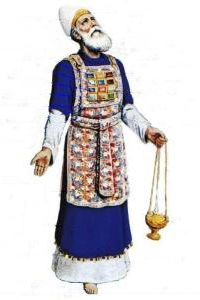
\includegraphics[width=50mm,scale=1.5]{Extras/Melchisedec.jpg}
\vspace{0.4in}  % Create a title for the document and write it in bold font
\LARGE{\textbf{\date}} % Again, do a line break
\linebreak 
% Create a subtitle \large{with Outlines, Statistics, Cross References, and Notes}
\vspace{0.5in}
\begin{flushleft}
\LARGE{Day \#72: Monday, 14 March 2022  \\}\vspace{0.25in}
\LARGE{Judges 1-3 Psalm 73 Proverb 14}
\end{flushleft}
\vspace{0.6in}
\bigskip

\normalsize{Xenia, Oh.\\}
\normalsize{created: \today}
\vspace{1.3in}

\end{flushright}
\end{titlepage}

\newpage 
\tableofcontents\hypertarget{TOC}{}
\listoffigures
\listoftables

\hyphenation{A-bim-e-lech bre-thren E-phra-im  Gib-e-o-nites Jer-u-sa-lem through-out Phil-i-stines The-o-phil-us Am-a-le-kites ven-geance Mesh-el-e-mi-ah onan-ism Phar-a-oh thoughts grev-ous-ness Hach-a-liah adul-ter-er Shad-rach}

%%%%%%%%%%%%%%%%% EXTRA COLORS
%%%%%%%%%%%%%%%%% EXTRA COLORS
%%%%%%%%%%%%%%%%% EXTRA COLORS
\definecolor{champagne}{rgb}{0.97,0.91,0.81}
\definecolor{bone}{rgb}{0.89,0.85,0.79}

\definecolor{ForestGreen}{rgb}{0.00,0.29,0.098}
\definecolor{GIVING}{cmyk}{1,0.0,0.72,.1}

\definecolor{MLPE}{cmyk}{1,1,0,.45}
\definecolor{SOCCER}{cmyk}{.77, 0, .42, .49}
\definecolor{PAYBILL}{cmyk}{0,0.83,0.76,0.07}
\definecolor{SERMON}{cmyk}{.14,.9,0,.30} % aka seance \href{http://www.flatuicolorpicker.com/purple-cmyk-color-model/}{seance}
\definecolor{BIBLE}{cmyk}{0,.17,.74,.17}
\definecolor{WORKBLUE}{cmyk}{1, .5, 0, .6}
\definecolor{myOrange}{cmyk}{0, .4, .98, .03}
\definecolor{myTan}{cmyk}{0.0,.07,.17,.10}
\definecolor{myRed}{cmyk}{0,1,1,0}
\definecolor{myWhite}{cmyk}{0,0,0,0}
\definecolor{BLUESoD}{cmyk}{.97,.84,0,.04}
\definecolor{WHITE}{cmyk}{0,0,0,0}
\definecolor{OLDGOLD}{cmyk}{0.05,0.3,1.00,0}
\definecolor{CASTLETON}{cmyk}{1,0,0.31,0.66}
\definecolor{cadmiumgreen}{rgb}{0.0, 0.42, 0.24}
\definecolor{jungle}{rgb}{0.203,0.4882,0.1718}
\definecolor{MYGOLD}{rgb}{1,.84,0}

\definecolor{MYLIGHTGRAY}{rgb}{.85,.85,.85}

\definecolor{codegreen}{rgb}{0,0.6,0}
\definecolor{codegray}{rgb}{0.5,0.5,0.5}
\definecolor{codepurple}{rgb}{0.58,0,0.82}
\definecolor{backcolour}{rgb}{0.95,0.95,0.92}


\mdfdefinestyle{MyFrame}{%
    linecolor=blue,
    outerlinewidth=2pt,
    roundcorner=5pt,
    innertopmargin=\baselineskip,
    innerbottommargin=\baselineskip,
    innerrightmargin=10pt,
    innerleftmargin=10pt,
    backgroundcolor=gray!25!white}


\mdfdefinestyle{MyFrame2}{%
    linecolor=black,
    outerlinewidth=2pt,
    roundcorner=5pt,
    innertopmargin=\baselineskip,
    innerbottommargin=\baselineskip,
    innerrightmargin=10pt,
    innerleftmargin=10pt,
    backgroundcolor=yellow!25!white}


%%%%%
%% for PFTTIS list
%%%%%

%%% And Joseph said unto
\index[PFTTIS]{And Joseph said unto!Genesis!Gen 40:008}
\index[PFTTIS]{And Joseph said unto!Genesis!Gen 40:012}
\index[PFTTIS]{And Joseph said unto!Genesis!Gen 41:025}
\index[PFTTIS]{And Joseph said unto!Genesis!Gen 42:014}
\index[PFTTIS]{And Joseph said unto!Genesis!Gen 42:018}
\index[PFTTIS]{And Joseph said unto!Genesis!Gen 44:015}
\index[PFTTIS]{And Joseph said unto!Genesis!Gen 45:003}
\index[PFTTIS]{And Joseph said unto!Genesis!Gen 45:004}
\index[PFTTIS]{And Joseph said unto!Genesis!Gen 46:031}
\index[PFTTIS]{And Joseph said unto!Genesis!Gen 48:009}
\index[PFTTIS]{And Joseph said unto!Genesis!Gen 48:018}
\index[PFTTIS]{And Joseph said unto!Genesis!Gen 50:019}
\index[PFTTIS]{And Joseph said unto!Genesis!Gen 50:024}


%%% a shadow
\index[PFTTIS]{a shadow!1Chronicles!1Chr 029:15}
\index[PFTTIS]{a shadow!Job!Job 008:09}
\index[PFTTIS]{a shadow!Job!Job 014:02}
\index[PFTTIS]{a shadow!Job!Job 017:07}
\index[PFTTIS]{a shadow!Psalm!Psa 102:011}
\index[PFTTIS]{a shadow!Psalm!Psa 144:004}
\index[PFTTIS]{a shadow!Ecclesiastes!Eccl 006:012}
\index[PFTTIS]{a shadow!Ecclesiastes!Eccl 008:013}
\index[PFTTIS]{a shadow!Isaiah!Isa 04:006}
\index[PFTTIS]{a shadow!Isaiah!Isa 25:004}
\index[PFTTIS]{a shadow!Jonah!Jnh 04:06}
\index[PFTTIS]{a shadow!Colossians!Col 02:017}
\index[PFTTIS]{a shadow!Hebews!Heb 10:001}

%%% blessed is the man
\index[PFTTIS]{blessed is the man!Psalm!Psa 001:001}
\index[PFTTIS]{blessed is the man!Psalm!Psa 032:002}
\index[PFTTIS]{blessed is the man!Psalm!Psa 034:008}
\index[PFTTIS]{blessed is the man!Psalm!Psa 065:004}
\index[PFTTIS]{blessed is the man!Psalm!Psa 084:005}
\index[PFTTIS]{blessed is the man!Psalm!Psa 084:012}
\index[PFTTIS]{blessed is the man!Psalm!Psa 094:012}
\index[PFTTIS]{blessed is the man!Psalm!Psa 112:001}
\index[PFTTIS]{blessed is the man!Proverbs!Pro 008:034}
\index[PFTTIS]{blessed is the man!Isaiah!Isa 056:002}
\index[PFTTIS]{blessed is the man!Jeremiah!Jer 017:007}
\index[PFTTIS]{blessed is the man!Romans!Rom 004:008}
\index[PFTTIS]{blessed is the man!James!Jam 001:012}


%%% carry them
\index[PFTTIS]{carry them!Leviticus!Lev 14:045}
\index[PFTTIS]{carry them!Numbers!Num 11:012}
\index[PFTTIS]{carry them!Joshua!Jsh 04:003}
\index[PFTTIS]{carry them!1Samuel!1Sam 20:040}
\index[PFTTIS]{carry them!1Kings!1Kng 08:046}
\index[PFTTIS]{carry them!2Chronicles!2Chr 06:036}
\index[PFTTIS]{carry them!Ezra!Ezra 05:015}
\index[PFTTIS]{carry them!Isaiah!Isa 40:011}
\index[PFTTIS]{carry them!Isaiah!Isa 41:016}
\index[PFTTIS]{carry them!Isaiah!Isa 57:013}
\index[PFTTIS]{carry them!Jeremiah!Jer 20:004}
\index[PFTTIS]{carry them!Jeremiah!Jer 20:005}
\index[PFTTIS]{carry them!Jeremiah!Jer 43:012}


\index[PFTTIS]{good tidings!2Samuel!2Sam 18:027}
\index[PFTTIS]{good tidings!1Kings!1Ki 01:042}
\index[PFTTIS]{good tidings!2Kings!2Ki 07:009 (2x)}
\index[PFTTIS]{good tidings!Isaiah!Isa 40:009 (2x)}
\index[PFTTIS]{good tidings!Isaiah!Isa 41:007}
\index[PFTTIS]{good tidings!Isaiah!Isa 52:007}
\index[PFTTIS]{good tidings!Isaiah!Isa 61:001}
\index[PFTTIS]{good tidings!Nahum!Nah 01:005}
\index[PFTTIS]{good tidings!Luke!Lk 02:010}
\index[PFTTIS]{good tidings!1Thessalonians!1Thess 03:006}


%%% dead body
\index[PFTTIS]{dead body!Leviticus!Lev 21:011}
\index[PFTTIS]{dead body!Numbers!Num 06:006}
\index[PFTTIS]{dead body!Numbers!Num 09:006}
\index[PFTTIS]{dead body!Numbers!Num 09:007}
\index[PFTTIS]{dead body!Numbers!Num 09:010}
\index[PFTTIS]{dead body!Numbers!Num 09:011}
\index[PFTTIS]{dead body!Numbers!Num 09:013}
\index[PFTTIS]{dead body!Numbers!Num 09:016}
\index[PFTTIS]{dead body!2Kings!2Ki 08:005}
\index[PFTTIS]{dead body!Isaiah!Isa 26:019}
\index[PFTTIS]{dead body!Jeremiah!Jer 26:023}
\index[PFTTIS]{dead body!Jeremiah!Jer 36:030}
\index[PFTTIS]{dead body!Haggai!Hag 02:013}

%%% great sea
\index[PFTTIS]{great sea!Numbers!Num 34:006}
\index[PFTTIS]{great sea!Numbers!Num 34:007}
\index[PFTTIS]{great sea!Joshua!Jos 01:004}
\index[PFTTIS]{great sea!Joshua!Jos 09:001}
\index[PFTTIS]{great sea!Joshua!Jos 15:012}
\index[PFTTIS]{great sea!Joshua!Jos 15:047}
\index[PFTTIS]{great sea!Joshua!Jos 23:004}
\index[PFTTIS]{great sea!Ezekiel!Eze 47:010}
\index[PFTTIS]{great sea!Ezekiel!Eze 47:015}
\index[PFTTIS]{great sea!Ezekiel!Eze 47:019}
\index[PFTTIS]{great sea!Ezekiel!Eze 47:020}
\index[PFTTIS]{great sea!Ezekiel!Eze 48:028}
\index[PFTTIS]{great sea!Daniel!Dan 07:002}


%%% have forsaken me
\index[PFTTIS]{have forsaken me!Judges!Jdg 10:013}
\index[PFTTIS]{have forsaken me!1Samuel!1Sam 08:008}
\index[PFTTIS]{have forsaken me!1Kings!1Ki 11:033}
\index[PFTTIS]{have forsaken me!2Kings!2Ki 22:017}
\index[PFTTIS]{have forsaken me!2Chronicles!2Chr 12:005}
\index[PFTTIS]{have forsaken me!2Chronicles!2Chr 34:025}
\index[PFTTIS]{have forsaken me!Jeremiah!Jer 01:016}
\index[PFTTIS]{have forsaken me!Jeremiah!Jer 02:013}
\index[PFTTIS]{have forsaken me!Jeremiah!Jer 05:007}
\index[PFTTIS]{have forsaken me!Jeremiah!Jer 05:019}
\index[PFTTIS]{have forsaken me!Jeremiah!Jer 16:011 (2x)}
\index[PFTTIS]{have forsaken me!Jeremiah!Jer 19:004}

%%% no king
\index[PFTTIS]{no king!Judges!Jdg 17:06}
\index[PFTTIS]{no king!Judges!Jdg 18:01}
\index[PFTTIS]{no king!Judges!Jdg 19:01}
\index[PFTTIS]{no king!Judges!Jdg 21:25}
\index[PFTTIS]{no king!1Kings!1Ki 22:47}
\index[PFTTIS]{no king!2Kings!2Ki 23:25}
\index[PFTTIS]{no king!Nehemiah!Neh 13:26}
\index[PFTTIS]{no king!Psalms!Psa 033:016}
\index[PFTTIS]{no king!Proverbs!Pro 30:27}
\index[PFTTIS]{no king!Daniel!Dan 02:10}
\index[PFTTIS]{no king!Hosea!Hos 10:03}
\index[PFTTIS]{no king!Micah!Mic 04:09}
\index[PFTTIS]{no king!John!Jhn 19:15}


%%% rebellious house
\index[PFTTIS]{rebellious house!Exodus!Exo 02:005}
\index[PFTTIS]{rebellious house!Exodus!Exo 02:006}
\index[PFTTIS]{rebellious house!Exodus!Exo 02:008}
\index[PFTTIS]{rebellious house!Exodus!Exo 03:009}
\index[PFTTIS]{rebellious house!Exodus!Exo 03:026}
\index[PFTTIS]{rebellious house!Exodus!Exo 03:027}
\index[PFTTIS]{rebellious house!Exodus!Exo 12:002 (2x)}
\index[PFTTIS]{rebellious house!Exodus!Exo 12:003}
\index[PFTTIS]{rebellious house!Exodus!Exo 12:009}
\index[PFTTIS]{rebellious house!Exodus!Exo 12:025}
\index[PFTTIS]{rebellious house!Exodus!Exo 17:012}
\index[PFTTIS]{rebellious house!Exodus!Exo 24:003}

%%% seek him
\index[PFTTIS]{seek him!Deuteronomy!Deu 04:029}\index[PFTTIS]{seek him!1Samuel!1Sam 23:025}
\index[PFTTIS]{seek him!1Chronicles!1Chr 28:009}
\index[PFTTIS]{seek him!2Chronicles!1Chr 15:002}
\index[PFTTIS]{seek him!Ezra!Ezr 08:022}
\index[PFTTIS]{seek him!Psalms!Psa 022:026}
\index[PFTTIS]{seek him!Psalms!Psa 024:006}
\index[PFTTIS]{seek him!Psalms!Psa 119:002}
\index[PFTTIS]{seek him!SoS!SoS 03:002}
\index[PFTTIS]{seek him!SoS!SoS 06:001}
\index[PFTTIS]{seek him!Hosea!Hos 07:010}
\index[PFTTIS]{seek him!Amos!Amo 05:008}
\index[PFTTIS]{seek him!Hebrews!Heb 11:0063}


%%% seek ye
\index[PFTTIS]{seek ye!Isaiah!Isa 34:016}
\index[PFTTIS]{seek ye!Isaiah!Isa 45:019}
\index[PFTTIS]{seek ye!Isaiah!Isa 55:006}
\index[PFTTIS]{seek ye!Amos!Amos 5:004}
\index[PFTTIS]{seek ye!John!John 1:38}
\index[PFTTIS]{seek ye!John!John 18:4}
\index[PFTTIS]{seek ye!John!John 18:7}
\index[PFTTIS]{seek ye!Matthew!Matt 6:33}
\index[PFTTIS]{seek ye!Numbers!Num 16:10}
\index[PFTTIS]{seek ye!Luke!Luke 12:31}
\index[PFTTIS]{seek ye!Luke!Luke 24:5}
\index[PFTTIS]{seek ye!Psalm!Psa 27:8}
\index[PFTTIS]{seek ye!Zephaniah!Zeph 2:3}

%%% the uncircumcised
\index[PFTTIS]{the uncircumcised!Genesis!Gen 17:014}
\index[PFTTIS]{the uncircumcised!Judges!Jdg 14:003}
\index[PFTTIS]{the uncircumcised!Judges!Jdg 15:018}
\index[PFTTIS]{the uncircumcised!2Samuel!2Sam 01:020}
\index[PFTTIS]{the uncircumcised!Isaiah!Isa 02:001}
\index[PFTTIS]{the uncircumcised!Jeremiah!Jer 09:025}
\index[PFTTIS]{the uncircumcised!Ezekiel!Eze 28:010}
\index[PFTTIS]{the uncircumcised!Ezekiel!Eze 31:018}
\index[PFTTIS]{the uncircumcised!Ezekiel!Eze 32:019}
\index[PFTTIS]{the uncircumcised!Ezekiel!Eze 32:027}
\index[PFTTIS]{the uncircumcised!Ezekiel!Eze 32:028}
\index[PFTTIS]{the uncircumcised!Ezekiel!Eze 32:029}
\index[PFTTIS]{the uncircumcised!Ezekiel!Eze 32:032}

%%% worship him
\index[PFTTIS]{worship him!Psalms!Psa 97:007}
\index[PFTTIS]{worship him!Zephaniah!Zeph 02:011}
\index[PFTTIS]{worship him!Matthew!Matt 02:002}
\index[PFTTIS]{worship him!Matthew!Matt 02:008}
\index[PFTTIS]{worship him!John!John 04:023}
\index[PFTTIS]{worship him!John!John 04:024 (2x)} 
\index[PFTTIS]{worship him!Acts!Acts 17:023}
\index[PFTTIS]{worship him!Hebrews!Heb 01:006}
\index[PFTTIS]{worship him!Revelation!Rev 04:010}
\index[PFTTIS]{worship him!Revelation!Rev 13:008}
\index[PFTTIS]{worship him!Revelation!Rev 14:007}
\index[PFTTIS]{worship him!Revelation!Rev 19:010}


%%%%%
%% for PFTTIS list
%%%%%

%%% afflictions
\index[WFTTIS]{afflictions!Psalms!Psa 34:019}
\index[WFTTIS]{afflictions!Psalms!Psa 132:001}
\index[WFTTIS]{afflictions!Acts!Acts 07:010}
\index[WFTTIS]{afflictions!Acts!Acts 20:023}
\index[WFTTIS]{afflictions!2Corinthians!2Cor 06:004}
\index[WFTTIS]{afflictions!Colossians!Col 01:024}
\index[WFTTIS]{afflictions!1Thessalonians!1Thess 03:003}
\index[WFTTIS]{afflictions!2Timothy!2Tim 01:008}
\index[WFTTIS]{afflictions!2Timothy!2Tim 03:011}
\index[WFTTIS]{afflictions!2Timothy!2Tim 04:005}
\index[WFTTIS]{afflictions!Hebrews!Heb 10:032}
\index[WFTTIS]{afflictions!Hebrews!Heb 10:033}
\index[WFTTIS]{afflictions!1Peter!1Pet 05:009}

%%% acsend
\index[WFTTIS]{acsend!Joshua!Jos 06:05}
\index[WFTTIS]{acsend!Psalm!Psa 024:003}
\index[WFTTIS]{acsend!Psalm!Psa 135:007}
\index[WFTTIS]{acsend!Psalm!Psa 139:008}
\index[WFTTIS]{acsend!Isaiah!Isa 14:013}
\index[WFTTIS]{acsend!Isaiah!Isa 14:014}
\index[WFTTIS]{acsend!Jeremiah!Jer 10:013}
\index[WFTTIS]{acsend!Jeremiah!Jer 51:016}
\index[WFTTIS]{acsend!Ezekiel!Eze 38:009}
\index[WFTTIS]{acsend!John!John 06:062}
\index[WFTTIS]{acsend!John!John 20:017}
\index[WFTTIS]{acsend!Romans!Rom 10:006}
\index[WFTTIS]{acsend!Revelation!Rev 17:008}

%%% Assyrian
\index[WFTTIS]{Assyrian!Isaiah!Isa 10:005}
\index[WFTTIS]{Assyrian!Isaiah!Isa 10:024}
\index[WFTTIS]{Assyrian!Isaiah!Isa 14:025}
\index[WFTTIS]{Assyrian!Isaiah!Isa 19:023}
\index[WFTTIS]{Assyrian!Isaiah!Isa 23:013}
\index[WFTTIS]{Assyrian!Isaiah!Isa 30:031}
\index[WFTTIS]{Assyrian!Isaiah!Isa 31:008}
\index[WFTTIS]{Assyrian!Isaiah!Isa 52:004}
\index[WFTTIS]{Assyrian!Ezekiel!Eze 31:003}
\index[WFTTIS]{Assyrian!Hosea!Hos 05:013}
\index[WFTTIS]{Assyrian!Hosea!Hos 11:005}
\index[WFTTIS]{Assyrian!Micah!Hos 05:005}
\index[WFTTIS]{Assyrian!Micah!Hos 05:006}

%%% blot
\index[WFTTIS]{blot!Exodus!Exo 32:032}
\index[WFTTIS]{blot!Exodus!Exo 32:033}
\index[WFTTIS]{blot!Numbers!Num 05:026}
\index[WFTTIS]{blot!Deuteronomy!Deut 09:014}
\index[WFTTIS]{blot!Deuteronomy!Deut 25:019}
\index[WFTTIS]{blot!Deuteronomy!Deut 29:020}
\index[WFTTIS]{blot!2Kings!2Ki 14:027}
\index[WFTTIS]{blot!Job!Job 31:007}
\index[WFTTIS]{blot!Psalms!Psa 51:001}
\index[WFTTIS]{blot!Psalms!Psa 51:009}
\index[WFTTIS]{blot!Proverbs!Pro 09:007}
\index[WFTTIS]{blot!Jeremiah!Jer 18:023}
\index[WFTTIS]{blot!Revelation!Rev 03:005}


%%% chain
\index[WFTTIS]{chain!Genesis!Gen 41:042}
\index[WFTTIS]{chain!1Kings!1Ki 07:017}
\index[WFTTIS]{chain!Psalms!Psa 73:006}
\index[WFTTIS]{chain!SoS!Sos 04:009}
\index[WFTTIS]{chain!Lamentations!Lam 03:007}
\index[WFTTIS]{chain!Ezekiel!Eze 07:023}
\index[WFTTIS]{chain!Ezekiel!Eze 16:011}
\index[WFTTIS]{chain!Daniel!Dan 05:007}
\index[WFTTIS]{chain!Daniel!Dan 05:016}
\index[WFTTIS]{chain!Daniel!Dan 05:029}
\index[WFTTIS]{chain!Acts!Acts 28:020}
\index[WFTTIS]{chain!2Timothy!2Tim 01:016}
\index[WFTTIS]{chain!Revelation!Rev 20:001}


%%% controversy
\index[WFTTIS]{controversy!Deuteronomy!Deu 17:008}
\index[WFTTIS]{controversy!Deuteronomy!Deu 19:017}
\index[WFTTIS]{controversy!Deuteronomy!Deu 21:005}
\index[WFTTIS]{controversy!Deuteronomy!Deu 25:001}
\index[WFTTIS]{controversy!2Samuel!2Sam 15:002}
\index[WFTTIS]{controversy!Isaiah!Isa 34:008}
\index[WFTTIS]{controversy!Jeremiah!Jer 25:031}
\index[WFTTIS]{controversy!Ezekiel!Eze 44:024}
\index[WFTTIS]{controversy!Hosea!Hos 04:001}
\index[WFTTIS]{controversy!Hosea!Hos 12:002}
\index[WFTTIS]{controversy!Micah!Mic 06:002 (2x)}
\index[WFTTIS]{controversy!1Timothy!1Tim 03:016}


%%% Dagon/Dagon's
\index[WFTTIS]{Dagon!Judges!Jdg 16:023}
\index[WFTTIS]{Dagon!1Samuel!1Sam 05:002 (2x)}
\index[WFTTIS]{Dagon!1Samuel!1Sam 05:003 (2x)}
\index[WFTTIS]{Dagon!1Samuel!1Sam 05:004 (3x)}
\index[WFTTIS]{Dagon!1Samuel!1Sam 05:005 (3x)}
\index[WFTTIS]{Dagon!1Samuel!1Sam 05:007}
\index[WFTTIS]{Dagon!1Chronicles!1Chr 10:010}

%%% disobedient
\index[WFTTIS]{disobedient!1Kings!1Ki 13:026}
\index[WFTTIS]{disobedient!Nehemiah!Neh 09:026}
\index[WFTTIS]{disobedient!Luke!Luke 01:017}
\index[WFTTIS]{disobedient!Acts!Acts 26:019}
\index[WFTTIS]{disobedient!Romans!Rom 01:030}
\index[WFTTIS]{disobedient!Romans!Rom 10:021}
\index[WFTTIS]{disobedient!1Timothy!1Tim 01:009}
\index[WFTTIS]{disobedient!2Timothy!2Tim 03:002}
\index[WFTTIS]{disobedient!Titus!Titus 01:016}
\index[WFTTIS]{disobedient!Titus!Titus 03:003}
\index[WFTTIS]{disobedient!1Peter!1Pet 02:007}
\index[WFTTIS]{disobedient!1Peter!1Pet 02:008}
\index[WFTTIS]{disobedient!1Peter!1Pet 03:020}


%%% doubt
\index[WFTTIS]{doubt!Genesis!Gen 37:033}
\index[WFTTIS]{doubt!Deuteronomy!Deu 28:066}
\index[WFTTIS]{doubt!Job!Job 12:002}
\index[WFTTIS]{doubt!Matthew!Matt 14:031}
\index[WFTTIS]{doubt!Matthew!Matt 21:021}
\index[WFTTIS]{doubt!Mark!Mk 11:023}
\index[WFTTIS]{doubt!Luke!Lk 11:020}
\index[WFTTIS]{doubt!John!Jhn 10:024}
\index[WFTTIS]{doubt!Acts!Acts 02:012}
\index[WFTTIS]{doubt!Acts!Acts 28:004}
\index[WFTTIS]{doubt!1Corinthians!1Cor 09:010}
\index[WFTTIS]{doubt!Galatians!Gal 04:020}
\index[WFTTIS]{doubt!1John!1Jhn 02:019}


%%% dungeon
\index[WFTTIS]{dungeon!Genesis!Gen 40:015}
\index[WFTTIS]{dungeon!Genesis!Gen 41:014}
\index[WFTTIS]{dungeon!Exodus!Exo 12:029}
\index[WFTTIS]{dungeon!Jeremiah!Jer 37:016}
\index[WFTTIS]{dungeon!Jeremiah!Jer 38:006 (2x)}
\index[WFTTIS]{dungeon!Jeremiah!Jer 38:007}
\index[WFTTIS]{dungeon!Jeremiah!Jer 38:009}
\index[WFTTIS]{dungeon!Jeremiah!Jer 38:010}
\index[WFTTIS]{dungeon!Jeremiah!Jer 38:011}
\index[WFTTIS]{dungeon!Jeremiah!Jer 38:013}
\index[WFTTIS]{dungeon!Lamentations!Lam 03:053}
\index[WFTTIS]{dungeon!Lamentations!Lam 03:055}


%%% error
\index[WFTTIS]{error!2Samuel!2Sam 06:007}
\index[WFTTIS]{error!Job!Job 19:004}
\index[WFTTIS]{error!Ecclesiastes!Ecc 05:006}
\index[WFTTIS]{error!Ecclesiastes!Ecc 10:005}
\index[WFTTIS]{error!Isaiah!Isa 32:006}
\index[WFTTIS]{error!Daniel!Dan 06:004}
\index[WFTTIS]{error!Matthew!Matt 27:064}
\index[WFTTIS]{error!Romans!Rom 01:027}
\index[WFTTIS]{error!James!Jam 05:020}
\index[WFTTIS]{error!2Peter!2Pet 02:018}
\index[WFTTIS]{error!2Peter!2Pet 03:017}
\index[WFTTIS]{error!1John!1Jn 04:006}
\index[WFTTIS]{error!Jude!Jude 01:011}

%%% fourish
\index[WFTTIS]{fourish!Psalms!Psa 072:007}
\index[WFTTIS]{fourish!Psalms!Psa 072:016}
\index[WFTTIS]{fourish!Psalms!Psa 092:007}
\index[WFTTIS]{fourish!Psalms!Psa 092:012}
\index[WFTTIS]{fourish!Psalms!Psa 092:013}
\index[WFTTIS]{fourish!Psalms!Psa 132:018}
\index[WFTTIS]{fourish!Proverbs!Pro 11:28}
\index[WFTTIS]{fourish!Proverbs!Pro 14:11}
\index[WFTTIS]{fourish!Ecclesiastes!Ecc 12:05}
\index[WFTTIS]{fourish!SongOfSolomon!SOS 07:12}
\index[WFTTIS]{fourish!Isaiah!Isa 17:11}
\index[WFTTIS]{fourish!Isaiah!Isa 66:14}
\index[WFTTIS]{fourish!Ezekiel!Eze 17:24}




%%% giants
\index[WFTTIS]{giants!Genesis!Gen 06:004}
\index[WFTTIS]{giants!Numbers!Num 13:033}
\index[WFTTIS]{giants!Deuteronomy!Deut 02:011}
\index[WFTTIS]{giants!Deuteronomy!Deut 02:021}
\index[WFTTIS]{giants!Deuteronomy!Deut 03:011}
\index[WFTTIS]{giants!Deuteronomy!Deut 03:013}
\index[WFTTIS]{giants!Joshua!Josh 12:004}
\index[WFTTIS]{giants!Joshua!Josh 13:012}
\index[WFTTIS]{giants!Joshua!Josh 15:008}
\index[WFTTIS]{giants!Joshua!Josh 17:015}
\index[WFTTIS]{giants!Joshua!Josh 16:016}

%%% good man
\index[WFTTIS]{good man!2 Samuel!2Sa 18:27}
%(1) Psalms 37:23 [5]
%(1) Psalms 112:5 [2]
%(1) Proverbs 12:2 [2]
%(1) Proverbs 13:22 [2]
%(1) Proverbs 14:14 [14]
%(1) Micah 7:2 [2]
%(1) Matthew 12:35 [2]
%(1) Luke 6:45 [2]
%(1) Luke 23:50 [15]
%(1) John 7:12 [17]
%(1) Acts 11:24 [5]
%(1) Romans 5:7 [14]

%%% Hinnom
\index[WFTTIS]{Hinnom!Joshua!Jsh 15:008}
\index[WFTTIS]{Hinnom!Joshua!Jsh 18:016}
\index[WFTTIS]{Hinnom!2Kings!2Ki 23:010}
\index[WFTTIS]{Hinnom!2Chronicles!2Chr 28:003}
\index[WFTTIS]{Hinnom!2Chronicles!2Chr 33:006}
\index[WFTTIS]{Hinnom!Nehemiah!Neh 11:030}
\index[WFTTIS]{Hinnom!Jeremiah!Jer 07:031}
\index[WFTTIS]{Hinnom!Jeremiah!Jer 07:032}
\index[WFTTIS]{Hinnom!Jeremiah!Jer 19:002}
\index[WFTTIS]{Hinnom!Jeremiah!Jer 19:006}
\index[WFTTIS]{Hinnom!Jeremiah!Jer 32:035}

%%% inclined
\index[WFTTIS]{inclined!Judges!Jdg 09:003}
\index[WFTTIS]{inclined!Psalms!Psa 040:001}
\index[WFTTIS]{inclined!Psalms!Psa 116:002}
\index[WFTTIS]{inclined!Psalms!Psa 119:112}
\index[WFTTIS]{inclined!Proverbs!Pro 05:13}
\index[WFTTIS]{inclined!Jeremiah!Jer 07:24}
\index[WFTTIS]{inclined!Jeremiah!Jer 07:26}
\index[WFTTIS]{inclined!Jeremiah!Jer 11:08}
\index[WFTTIS]{inclined!Jeremiah!Jer 17:23}
\index[WFTTIS]{inclined!Jeremiah!Jer 25:04}
\index[WFTTIS]{inclined!Jeremiah!Jer 34:14}
\index[WFTTIS]{inclined!Jeremiah!Jer 35:15}
\index[WFTTIS]{inclined!Jeremiah!Jer 44:05}


%%% laughed
\index[WFTTIS]{laughed!Genesis!Gen 17:017}
\index[WFTTIS]{laughed!Genesis!Gen 18:012}
\index[WFTTIS]{laughed!Genesis!Gen 18:015}
\index[WFTTIS]{laughed!2Kings!2Ki 19:021}
\index[WFTTIS]{laughed!2Chronicles!2Chr 30:010}
\index[WFTTIS]{laughed!Nehemiah!Neh 02:019}
\index[WFTTIS]{laughed!Job!Job 12:004}
\index[WFTTIS]{laughed!Job!Job 29:024}
\index[WFTTIS]{laughed!Isaiah!Isa 37:022}
\index[WFTTIS]{laughed!Ezekiel!Ezek 23:032}
\index[WFTTIS]{laughed!Matthew!Matt 09:024}
\index[WFTTIS]{laughed!Mark!Mk 05:040}
\index[WFTTIS]{laughed!Luke!Lk 08:053}

%%% liar
\index[WFTTIS]{liar!Job!Job 24:025}
\index[WFTTIS]{liar!Proverbs!Pro 17:004}
\index[WFTTIS]{liar!Proverbs!Pro 19:022}
\index[WFTTIS]{liar!Proverbs!Pro 30:006}
\index[WFTTIS]{liar!Jeremiah!Jer 15:018}
\index[WFTTIS]{liar!John!Jhn 08:044}
\index[WFTTIS]{liar!John!Jhn 08:055}
\index[WFTTIS]{liar!Romans!Rom 03:004}
\index[WFTTIS]{liar!1John!1Jhn 01:010}
\index[WFTTIS]{liar!1John!1Jhn 02:004}
\index[WFTTIS]{liar!1John!1Jhn 02:022}
\index[WFTTIS]{liar!1John!1Jhn 04:020}
\index[WFTTIS]{liar!1John!1Jhn 05:010}

%%% palsy
\index[WFTTIS]{palsy!Matthew!Matt 04:024}
\index[WFTTIS]{palsy!Matthew!Matt 08:006}
\index[WFTTIS]{palsy!Matthew!Matt 09:002}
\index[WFTTIS]{palsy!Matthew!Matt 09:006}
\index[WFTTIS]{palsy!Mark!Mk 02:003}
\index[WFTTIS]{palsy!Mark!Mk 02:004}
\index[WFTTIS]{palsy!Mark!Mk 02:005}
\index[WFTTIS]{palsy!Mark!Mk 02:009}
\index[WFTTIS]{palsy!Mark!Mk 02:010}
\index[WFTTIS]{palsy!Luke!Lk 05:018}
\index[WFTTIS]{palsy!Luke!Lk 05:024}
\index[WFTTIS]{palsy!Acts!Acts 09:033}

%%% Profitable
\index[WFTTIS]{profitable!Job!Job 22:002 (2x)}
\index[WFTTIS]{profitable!Ecclesiastes!Ecc 10:010}
\index[WFTTIS]{profitable!Isaiah!Isa 44:010}
\index[WFTTIS]{profitable!Jeremiah!Jer 13:007}
\index[WFTTIS]{profitable!Matthew!Matt 05:029}
\index[WFTTIS]{profitable!Matthew!Matt 05:030}
\index[WFTTIS]{profitable!Acts!Acts 20:020}
\index[WFTTIS]{profitable!1Timothy!1Tim 04:008}
\index[WFTTIS]{profitable!2Timothy!2Tim 03:016}
\index[WFTTIS]{profitable!2Timothy!2Tim 04:011}
\index[WFTTIS]{profitable!Titus!Titus 03:008}
\index[WFTTIS]{profitable!Philemon!Phlm 01:011}

%%% Rechab
\index[WFTTIS]{Rechab!2Samuel!2Sam 04:002}
\index[WFTTIS]{Rechab!2Samuel!2Sam 04:005}
\index[WFTTIS]{Rechab!2Samuel!2Sam 04:006}
\index[WFTTIS]{Rechab!2Samuel!2Sam 04:009}
\index[WFTTIS]{Rechab!2KIngs!2Ki 10:015}
\index[WFTTIS]{Rechab!2KIngs!2Ki 10:023}
\index[WFTTIS]{Rechab!1Chronicles!1Chr 02:055}
\index[WFTTIS]{Rechab!Nehemiah!Neh 03:014}
\index[WFTTIS]{Rechab!Jeremiah!Jer 35:006}
\index[WFTTIS]{Rechab!Jeremiah!Jer 35:008}
\index[WFTTIS]{Rechab!Jeremiah!Jer 35:014}
\index[WFTTIS]{Rechab!Jeremiah!Jer 35:016}
\index[WFTTIS]{Rechab!Jeremiah!Jer 35:019}

%%% serpents
\index[WFTTIS]{serpents!Exodus!Exo 07:012}
\index[WFTTIS]{serpents!Numbers!Num 21:006}
\index[WFTTIS]{serpents!Numbers!Num 21:007}
\index[WFTTIS]{serpents!Deuteronomy!Deu 08:015}
\index[WFTTIS]{serpents!Deuteronomy!Deu 32:024}
\index[WFTTIS]{serpents!Jeremiah!Jer 08:017}
\index[WFTTIS]{serpents!Matthew!Matt 10:016}
\index[WFTTIS]{serpents!Matthew!Matt 23:033}
\index[WFTTIS]{serpents!Mark!Mk 16:018}
\index[WFTTIS]{serpents!Luke!Lk 10:019}
\index[WFTTIS]{serpents!1Corinthians!1Cor 10:009}
\index[WFTTIS]{serpents!James!Jas 03:007}
\index[WFTTIS]{serpents!Revelation!Rev 09:019}

%%% short
\index[WFTTIS]{short!Numbers!Num 11:023}
\index[WFTTIS]{short!2Kings!2Ki 10:032}
\index[WFTTIS]{short!Job!Job 17:012}
\index[WFTTIS]{short!Job!Job 20:005}
\index[WFTTIS]{short!Psalms!Psa 89:047}
\index[WFTTIS]{short!Romans!Rom 03:023}
\index[WFTTIS]{short!Romans!Rom 09:028  (2x)}
\index[WFTTIS]{short!1Corinthians!1Cor 07:029}
\index[WFTTIS]{short!1Thessalonians!1Thess 02:017}
\index[WFTTIS]{short!Hebrews!Heb 04:001}
\index[WFTTIS]{short!Revelation!Rev 12:012}
\index[WFTTIS]{short!Revelation!Rev 17:010}

%%% smiteth
\index[WFTTIS]{smiteth!Exodus!Exo 21:012}
\index[WFTTIS]{smiteth!Exodus!Exo 21:15}
\index[WFTTIS]{smiteth!Deuteronomy!Dt 25:11}
\index[WFTTIS]{smiteth!Deuteronomy!Dt 27:24}
\index[WFTTIS]{smiteth!Joshua!Jsh 15:16}
\index[WFTTIS]{smiteth!Judges!Jdg 15:16}
\index[WFTTIS]{smiteth!2 Samuel!2Sa 05:08}
\index[WFTTIS]{smiteth!1Chronicles!1Chr 11:06}
\index[WFTTIS]{smiteth!Job!1Chr 26:12}
\index[WFTTIS]{smiteth!Isaiah!Isa 09:13}
\index[WFTTIS]{smiteth!Lamentations!Lam 03:30}
\index[WFTTIS]{smiteth!Ezekiel!Eze 07:09}
\index[WFTTIS]{smiteth!Luke!Lk 06:29}



%%% vanities
\index[WFTTIS]{vanities!Deuteronomy!Deut 21:021}
\index[WFTTIS]{vanities!1Kings!1Ki 16:013}
\index[WFTTIS]{vanities!1Kings!1Ki 16:026}
\index[WFTTIS]{vanities!Psalms!Psa 031:006}
\index[WFTTIS]{vanities!Ecclesiastes!Ecc 01:002 (2x)}
\index[WFTTIS]{vanities!Ecclesiastes!Ecc 05:007}
\index[WFTTIS]{vanities!Ecclesiastes!Ecc 12:008}
\index[WFTTIS]{vanities!Jeremiah!Jer 08:019}
\index[WFTTIS]{vanities!Jeremiah!Jer 10:008}
\index[WFTTIS]{vanities!Jeremiah!Jer 14:022}
\index[WFTTIS]{vanities!Jonah!Jnh 02:008}
\index[WFTTIS]{vanities!Acts!Acts 14:015}



%%%%%
%% for PFTTIS list
%%%%%

%%% worm
\index[WFITV]{worm!Exodus!Exo 16:024}
\index[WFITV]{worm!Job!Job 17:014}
\index[WFITV]{worm!Job!Job 24:029}
\index[WFITV]{worm!Job!Job 25:005 (2x)}
\index[WFITV]{worm!Psalms!Psa 022:006}
\index[WFITV]{worm!Isaiah!Isa 14:011}
\index[WFITV]{worm!Isaiah!Isa 41:014}
\index[WFITV]{worm!Isaiah!Isa 51:008}
\index[WFITV]{worm!Isaiah!Isa 66:024}
\index[WFITV]{worm!Jonah!Jnh 04:007}
\index[WFITV]{worm!Mark!Mk 09:044}
\index[WFITV]{worm!Mark!Mk 09:046}
\index[WFITV]{worm!Mark!Mk 09:048}


%\subsubsection{Title}
%\textbf{Introduction:} Isaiah 46 
%\index[speaker]{Speaker!Isaiah 49 (Title}
%\index[series]{Book (Speaker)!IPassage (Title)}
%\index[date]{2017/07/09!Isaiah 49 (Title)}
%\begin{compactenum}[I.]
%    \item  \textbf{Point} \index[scripture]{Isaiah!IPassage} (IPassage)
%\end{compactenum}




  


%\input{02OT-Exodus/ExodusIntroduction}

%\newpage
%\begin{figure}
%\begin{center}
%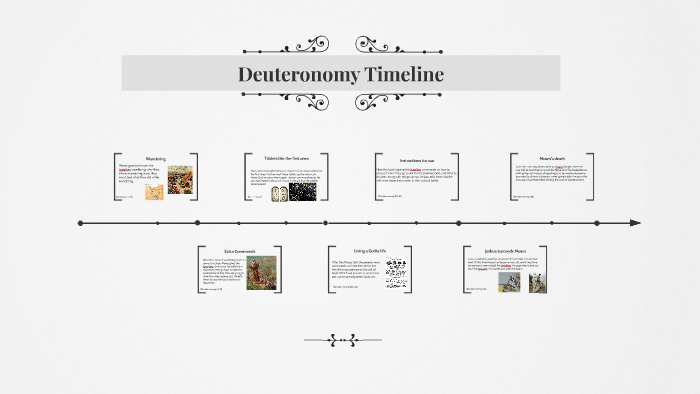
\includegraphics[scale=.7, angle=0]{05OT-Deuteronomy/References/AndrewSmithDeuteronomyTimeline.png}
%\caption[Deuteronomy Timeline by Andrew Smith]{Deuteronomy Timeline by Andrew %Smith}
%\label{fig:Deuteronomy Timeline by Andrew Smith}
%\end{center}
%\end{figure}

\newpage
\begin{figure}
\begin{center}
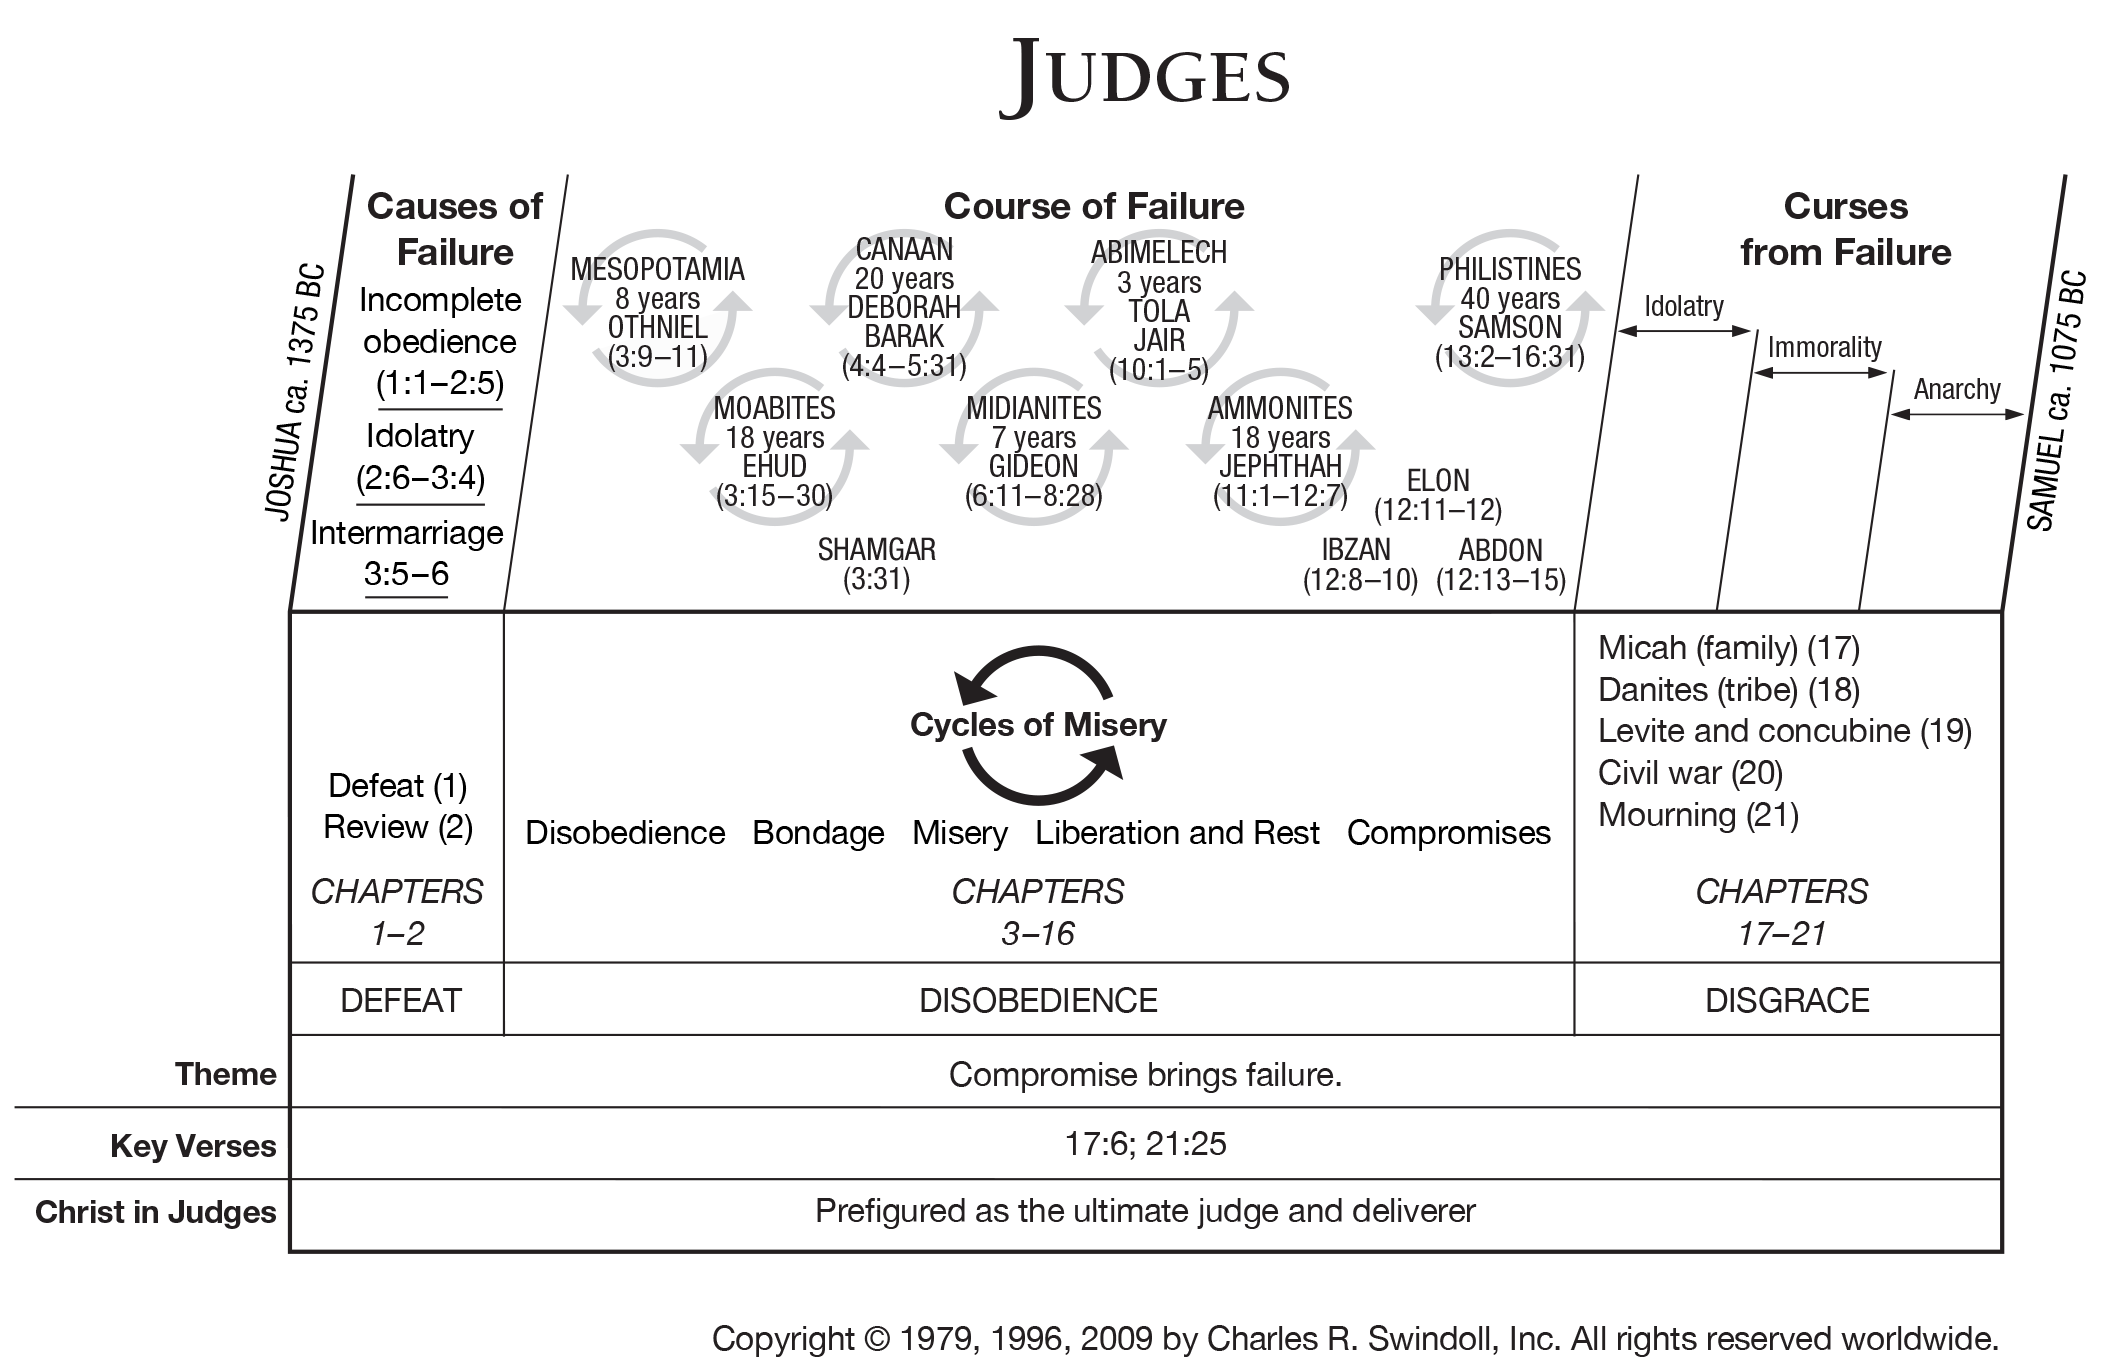
\includegraphics[scale=0.25, angle=90]{07OT-Judges/References/1.Judges-Swindoll}
\caption[Judges from Swindoll]{Judges from Swindoll}
\label{fig:Judges from Swindoll}
\end{center}
\end{figure}


%\newpage
%\begin{figure}
%\begin{center}
%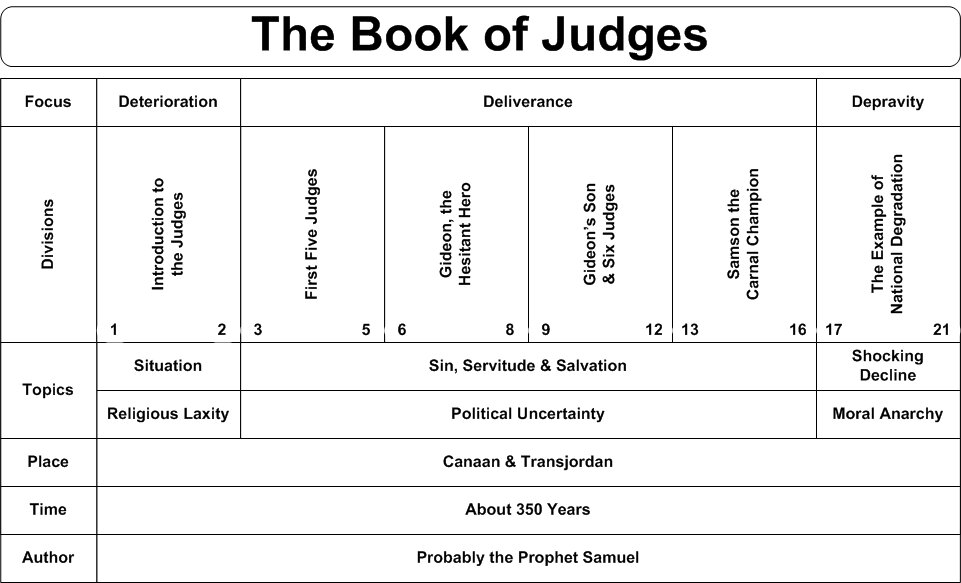
\includegraphics[scale=0.1, angle=0]{07OT-Judges/References/9.Swartzentrover-Judges}
%\caption[Judges from Swartzentrover]{Judges from Swartzentrover}
%\label{fig:Judges from Swartzentrover}
%\end{center}
%\end{figure}


\newpage
\begin{figure}
\begin{center}
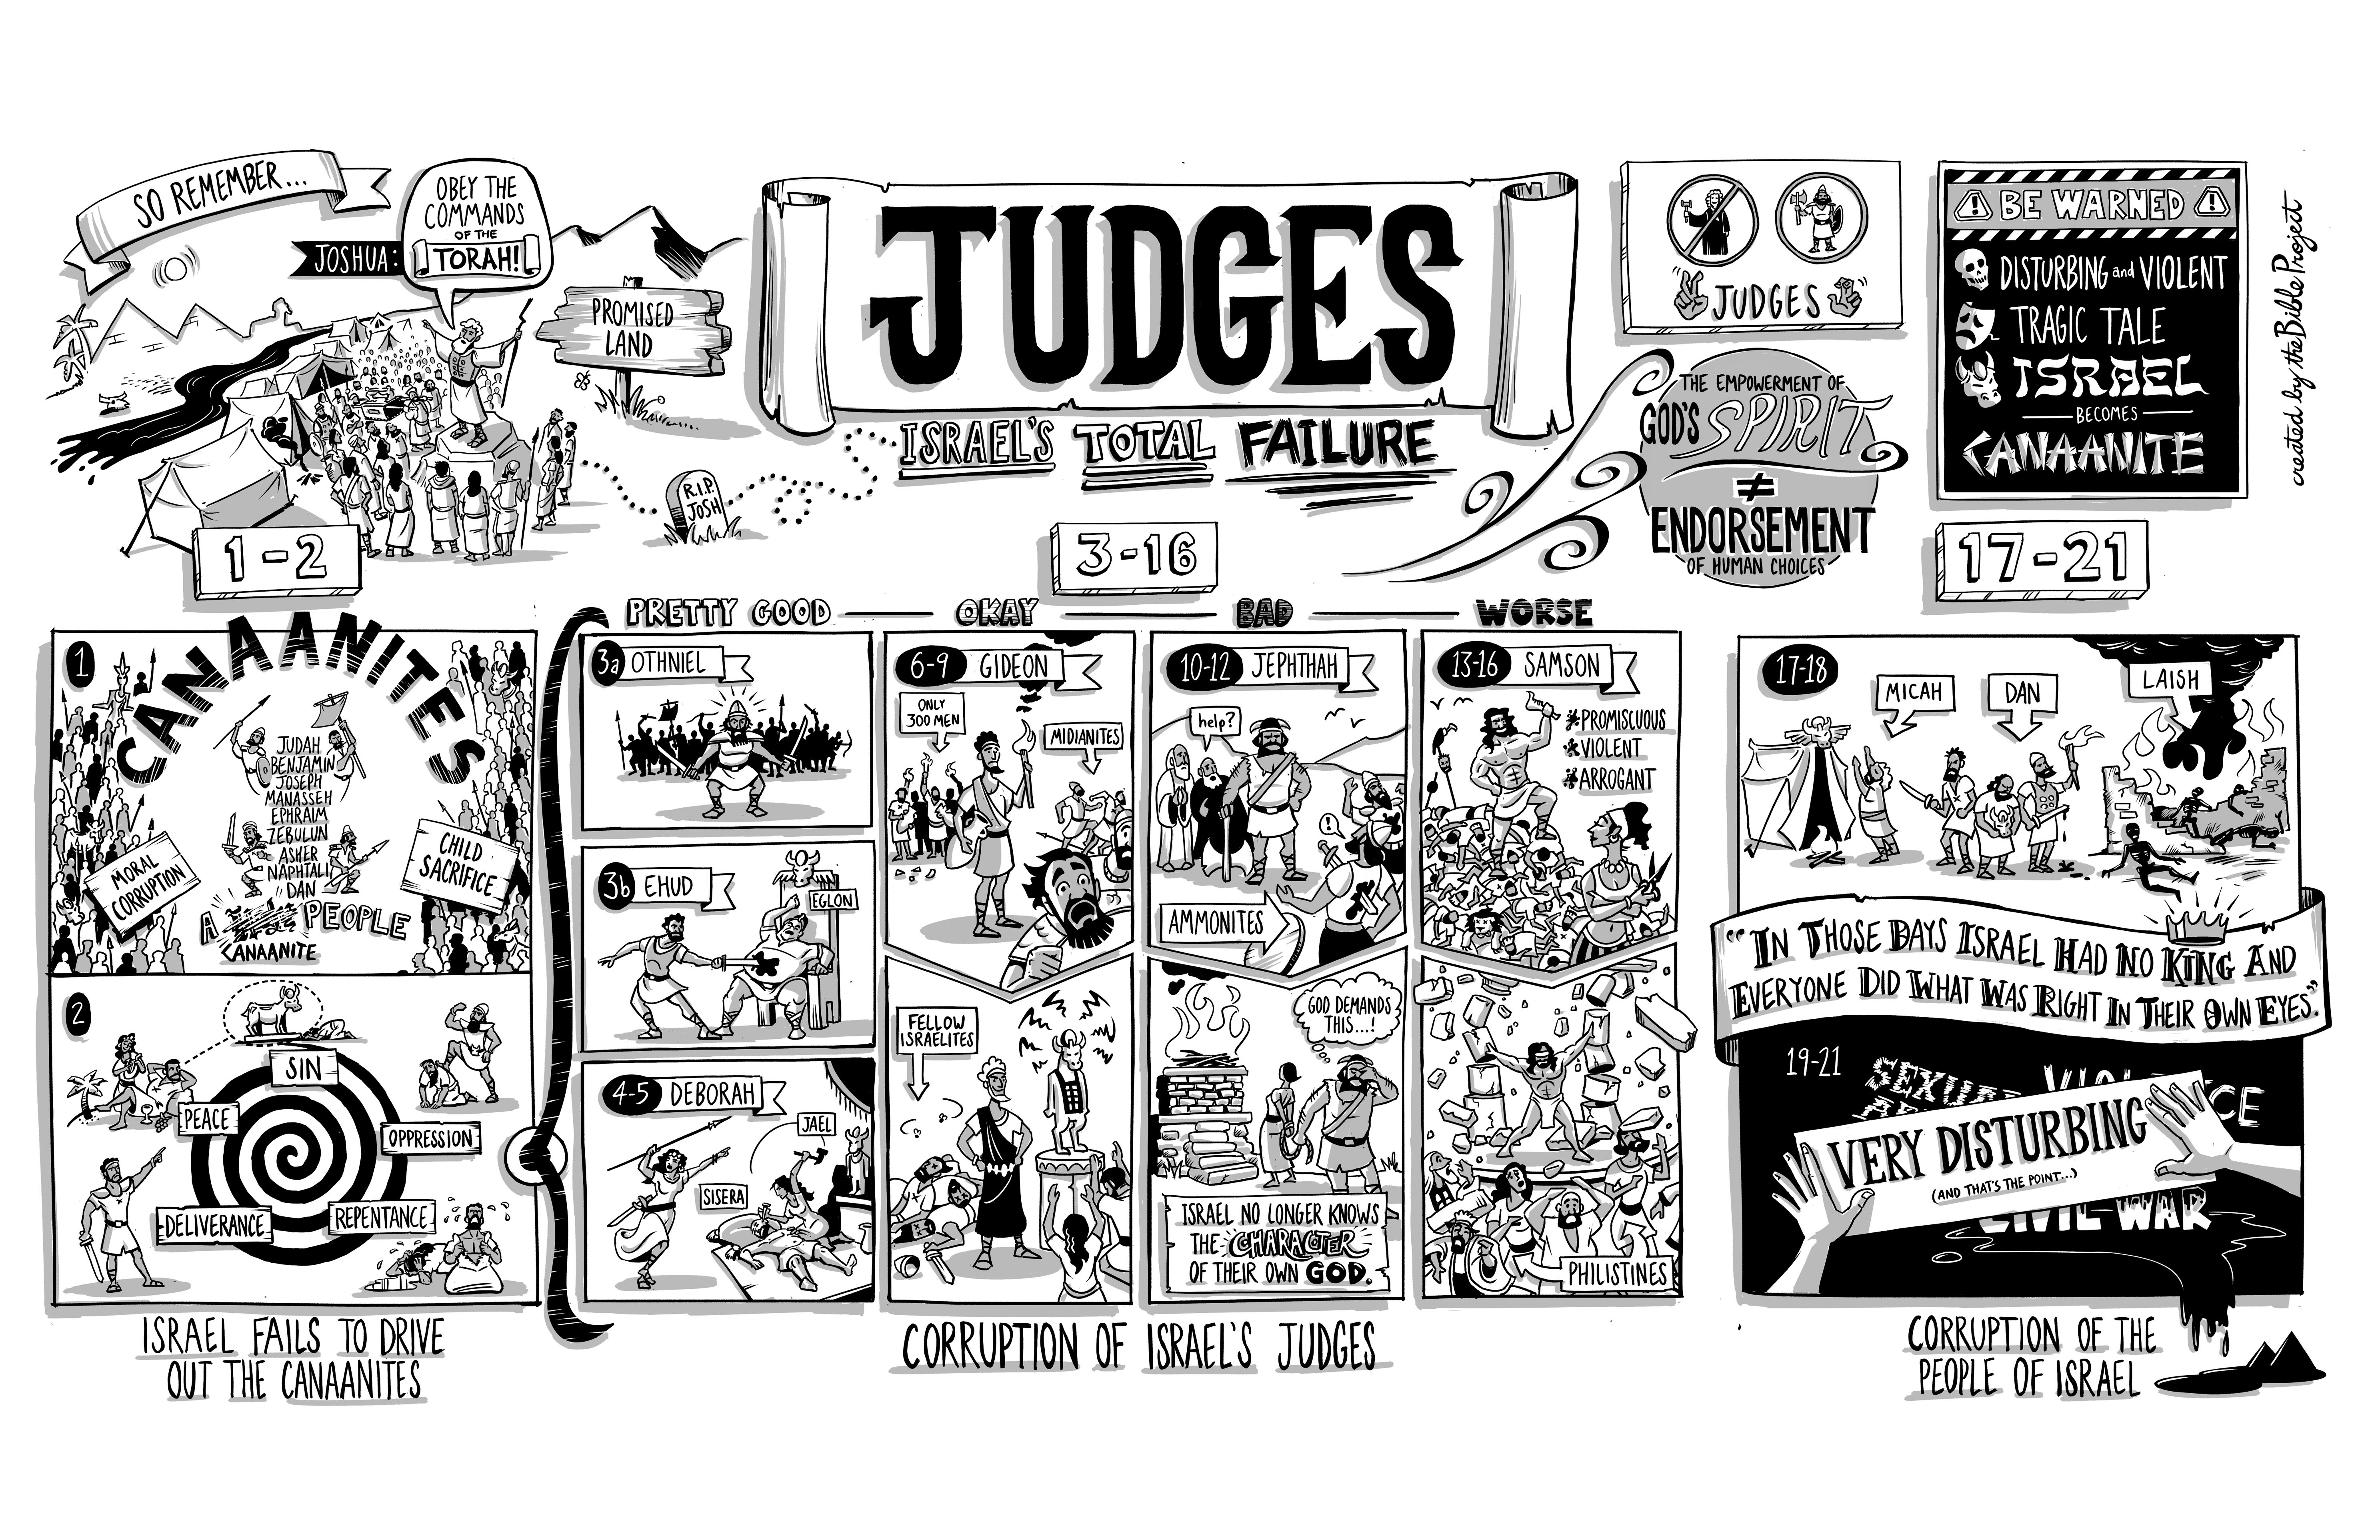
\includegraphics[scale=0.5, angle=90]{07OT-Judges/References/2.BibleProject-Judges}
\caption[Judges from the Bible Project]{Judges from the Bible Project}
\label{fig:Judges from the Bible Project}
\end{center}
\end{figure}


\newpage
\begin{figure}
\begin{center}
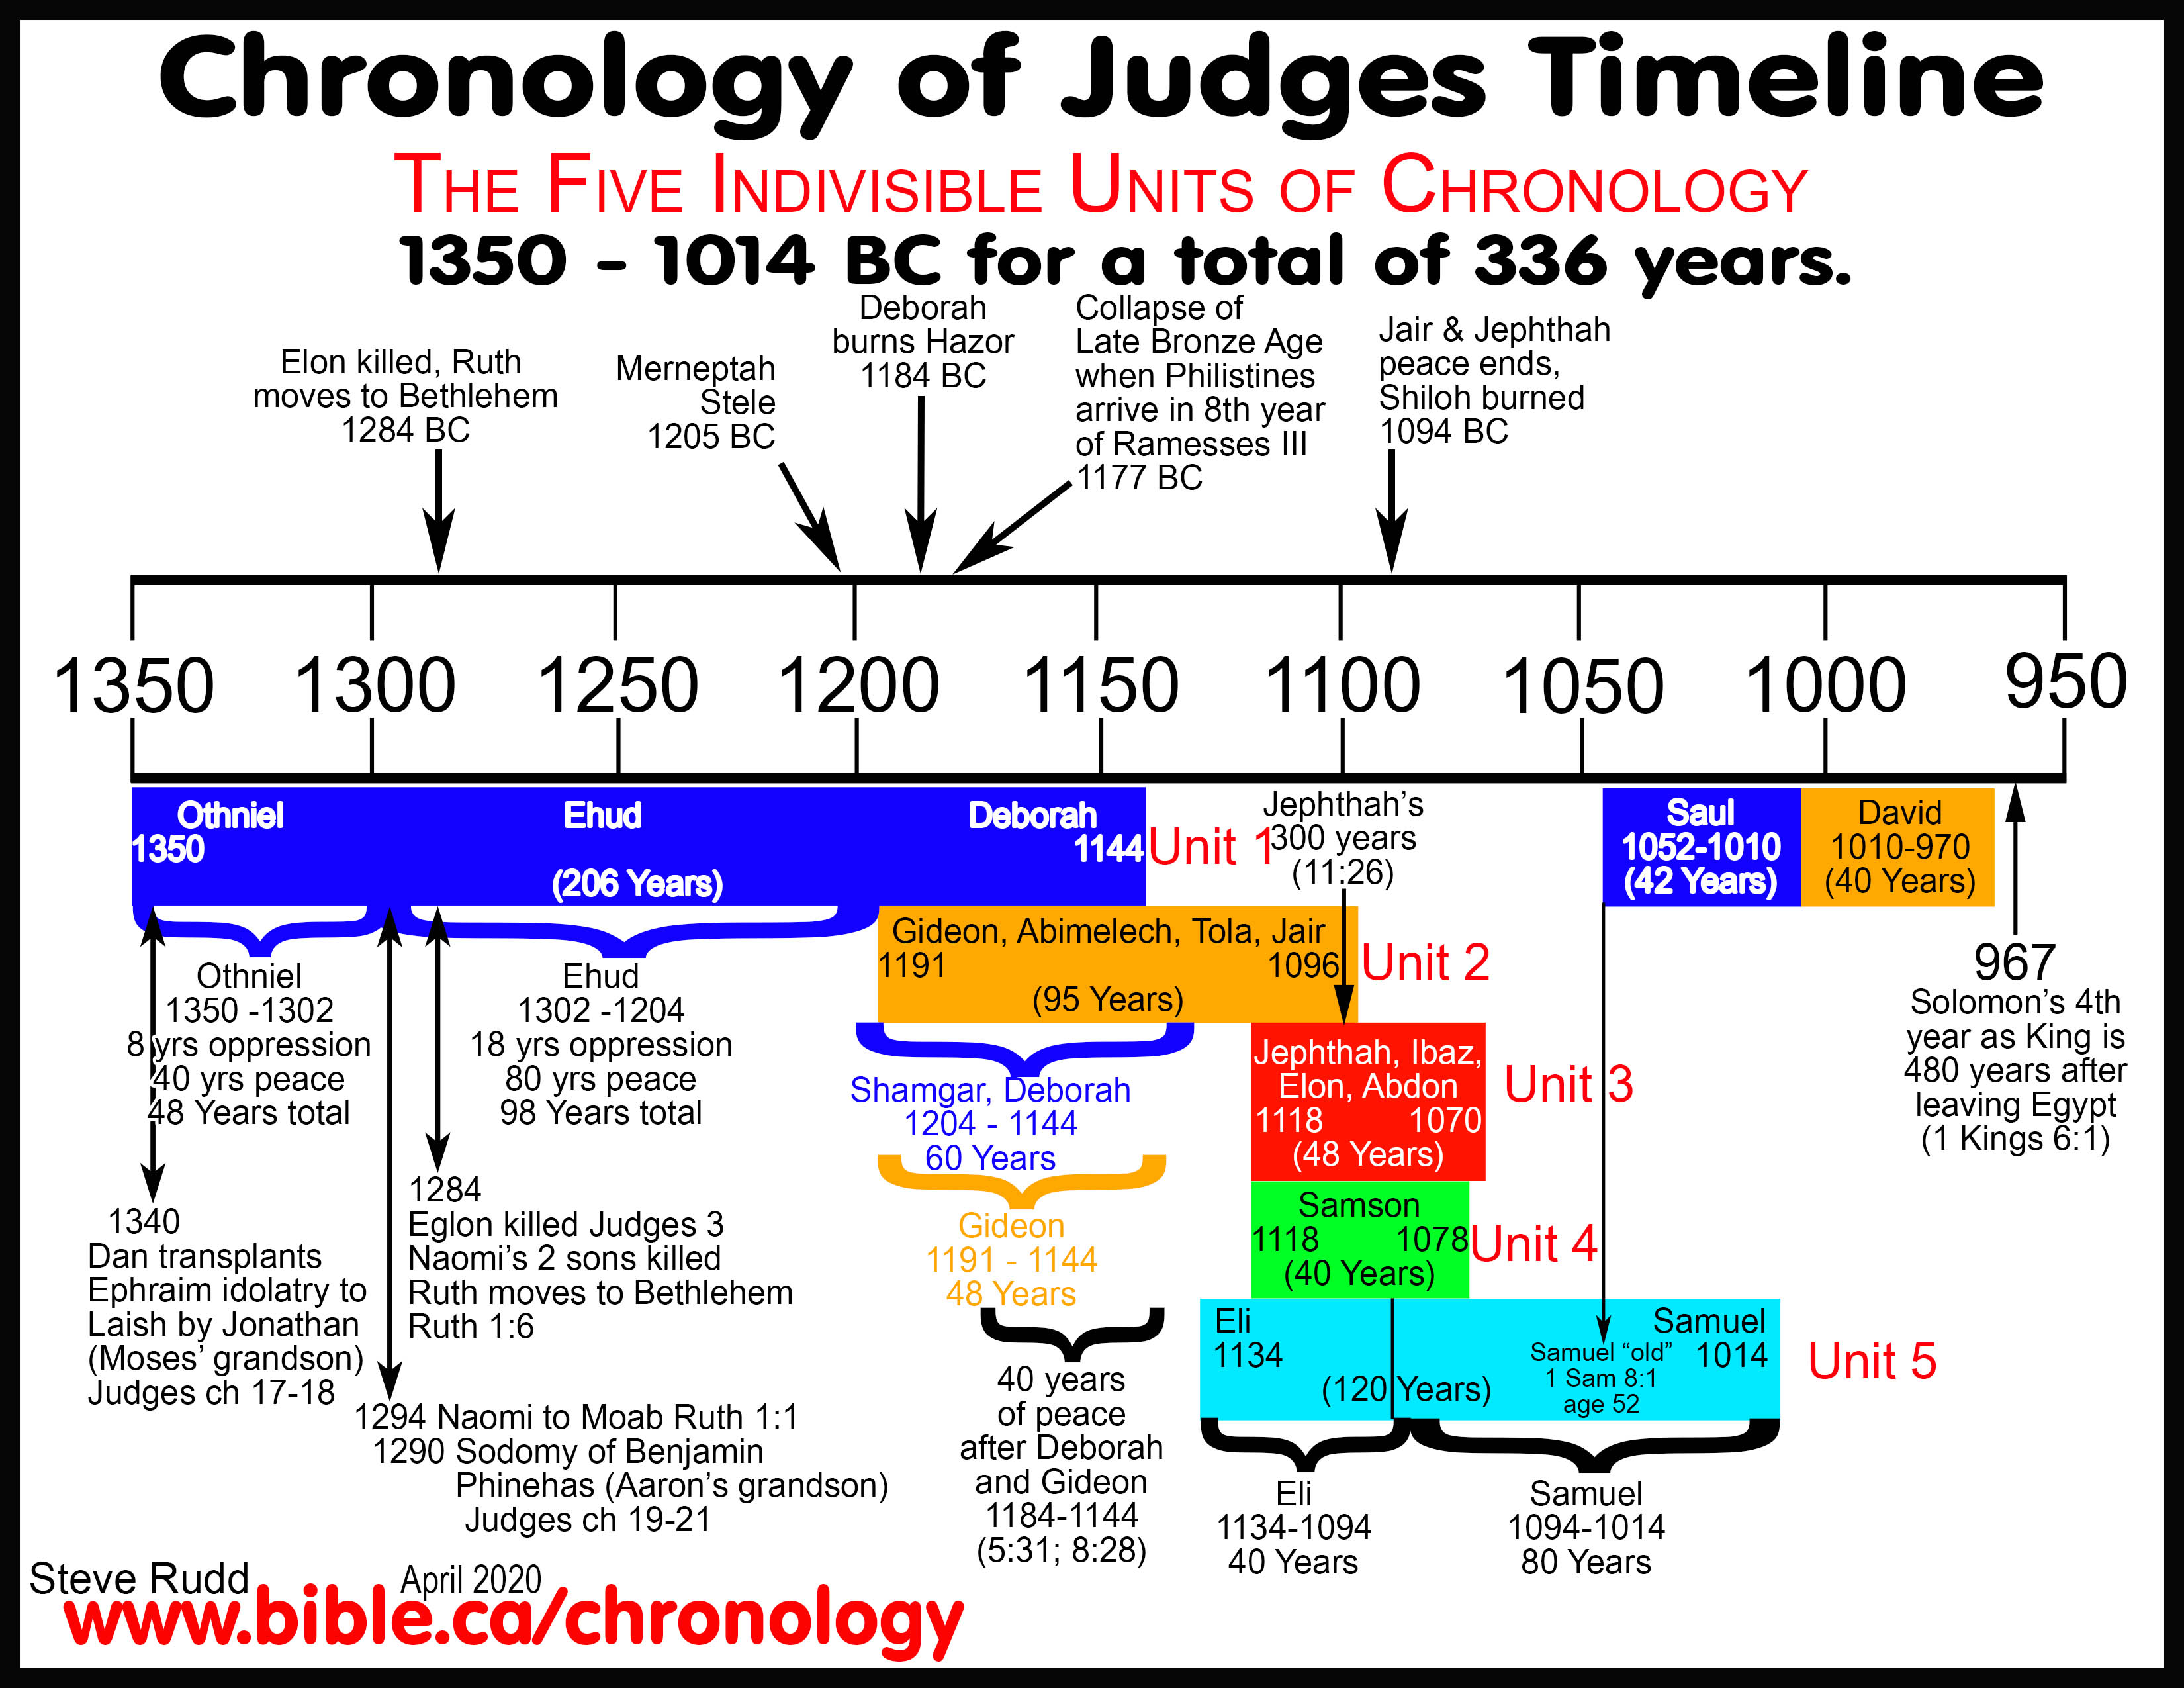
\includegraphics[scale=0.6, angle=90]{07OT-Judges/References/3.Chronology-Judges}
\caption[Chronology of Judges]{Chronology of Judges}
\label{fig:Chronology of Judges}
\end{center}
\end{figure}


\newpage
\begin{figure}
\begin{center}
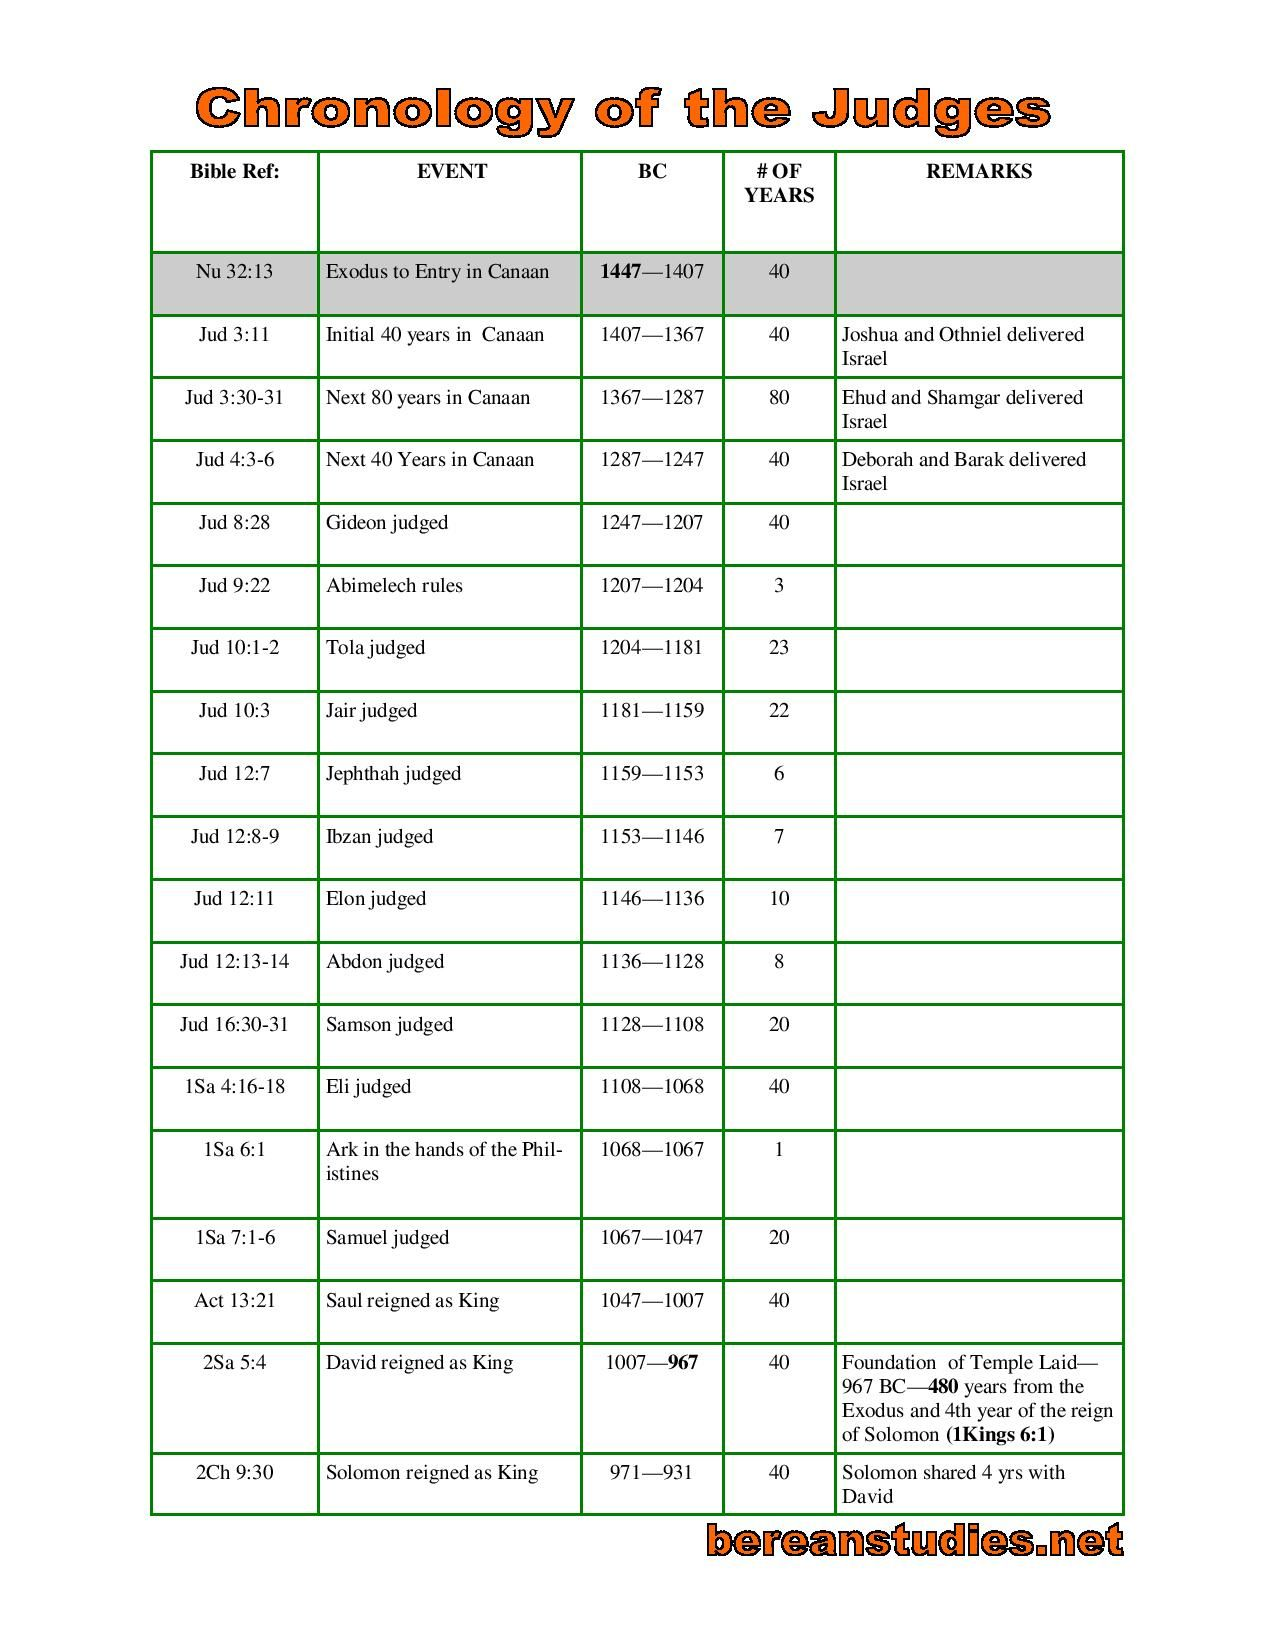
\includegraphics[scale=0.6, angle=0]{07OT-Judges/References/4.Chronology2-Judges}
\caption[Another Chronology of Judges]{Another Chronology of Judges}
\label{fig:Another Chronology of Judges}
\end{center}
\end{figure}

\newpage
\begin{figure}
\begin{center}
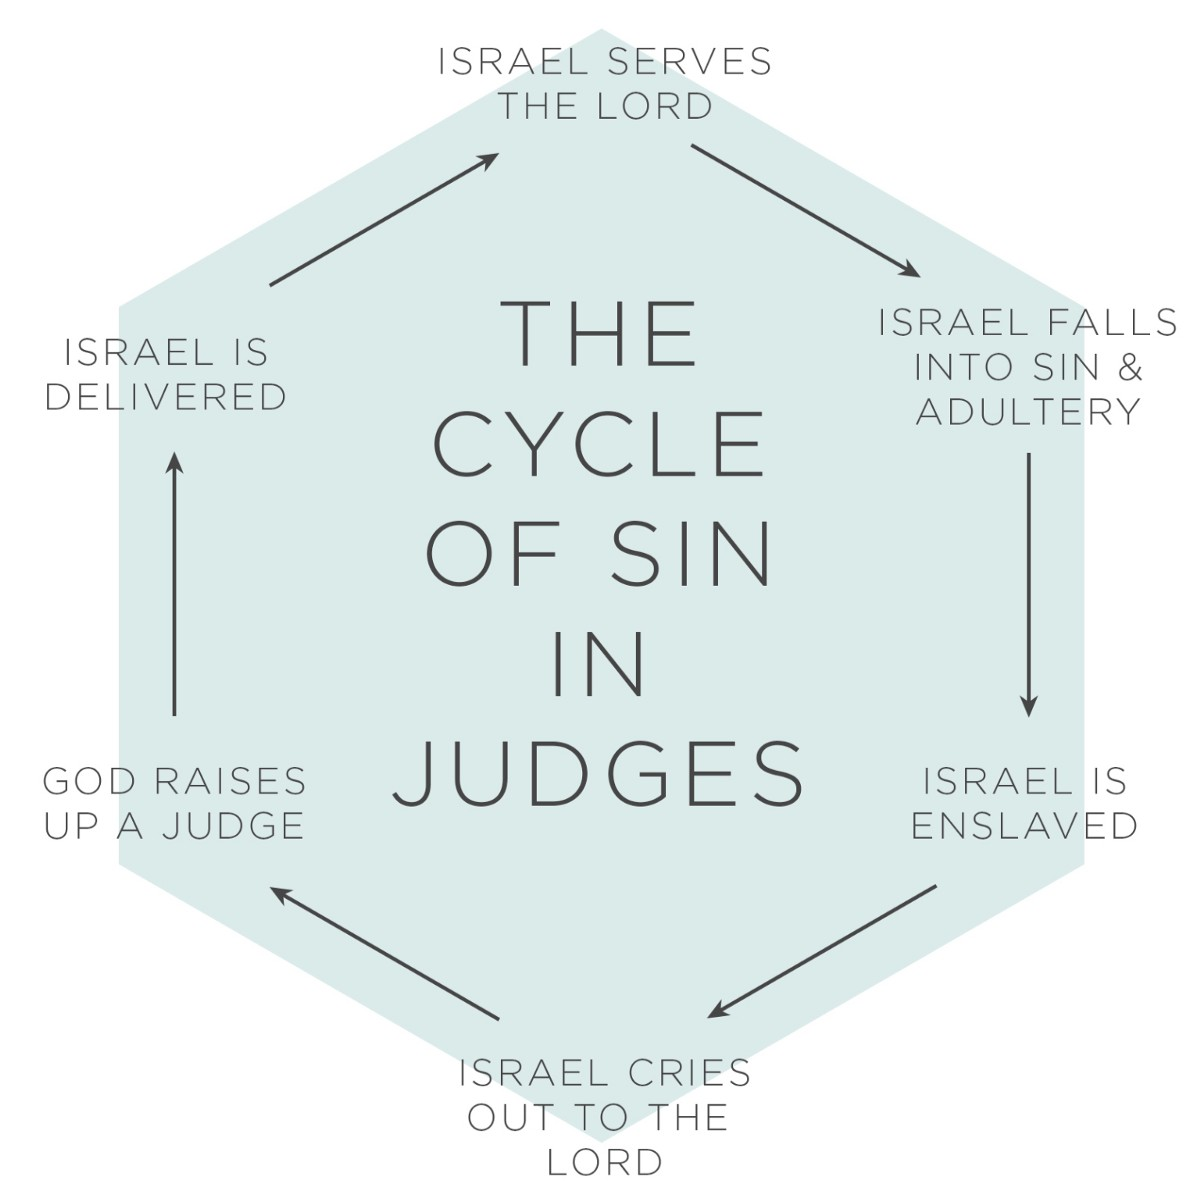
\includegraphics[scale=0.3, angle=0]{07OT-Judges/References/5.Cycles-Judges}
\caption[Cycle of Judges]{Cycle of Judges}
\label{fig:Cycle of Judges}
\end{center}
\end{figure}


\newpage
\begin{figure}
\begin{center}
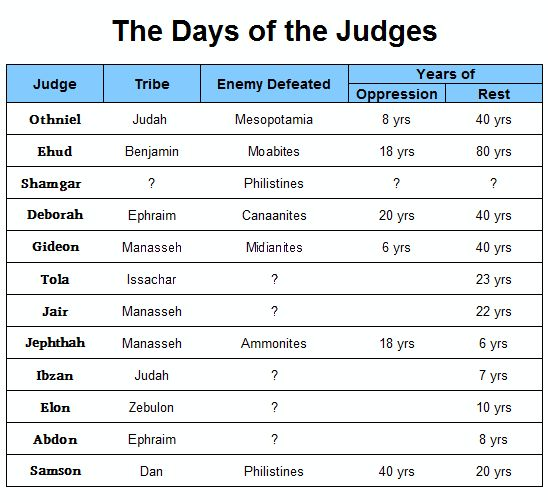
\includegraphics[scale=0.7, angle=0]{07OT-Judges/References/6.DaysOfJudges}
\caption[The Days of the Judges]{The Days of the Judges}
\label{fig:The Days of the Judges}
\end{center}
\end{figure}


\newpage
\begin{figure}
\begin{center}
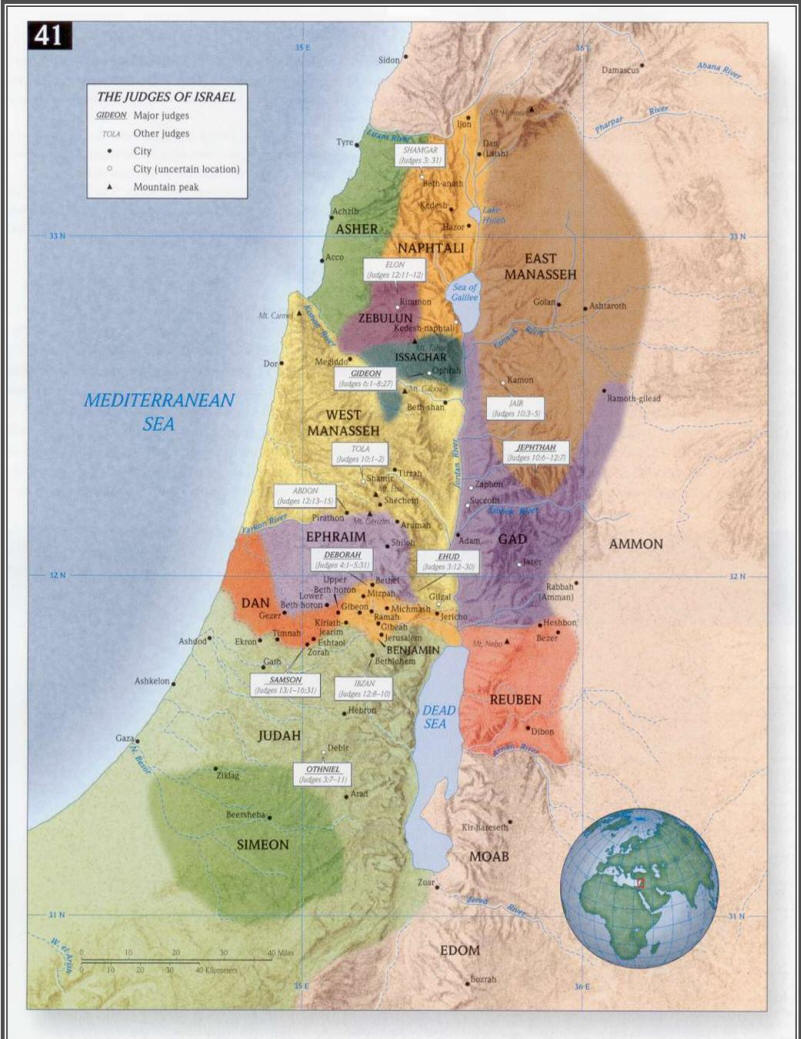
\includegraphics[scale=0.8, angle=0]{07OT-Judges/References/7.Map-Judges}
\caption[Map of the Judges]{Map of the Judges}
\label{fig:Map of the Judges}
\end{center}
\end{figure}


\newpage
\begin{figure}
\begin{center}
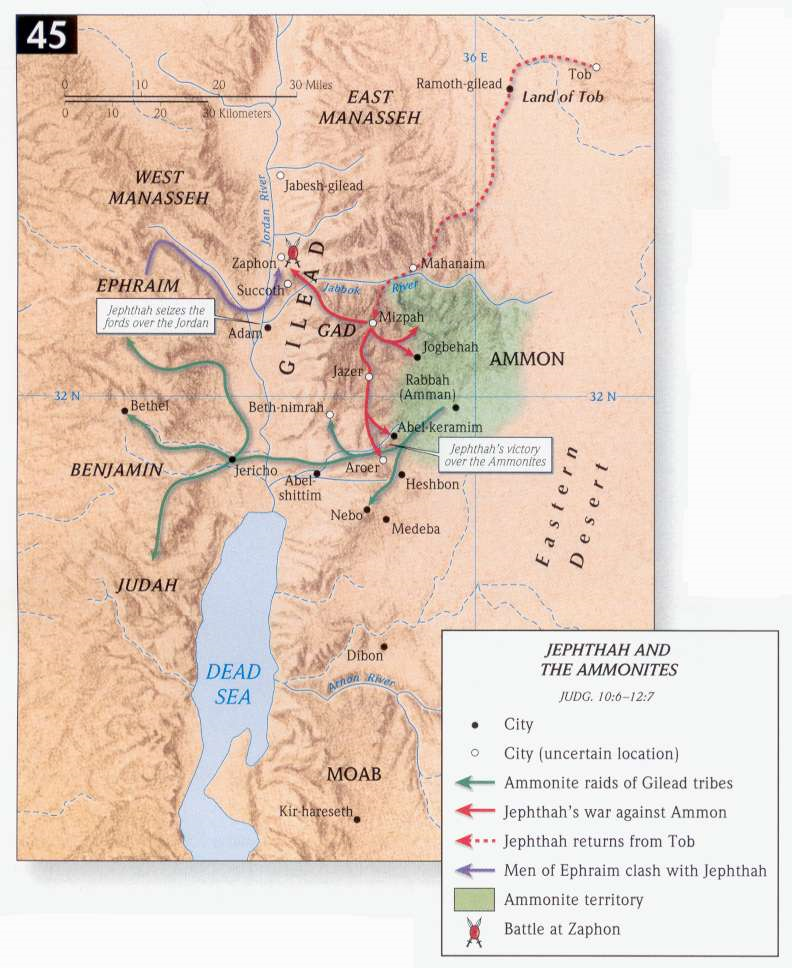
\includegraphics[scale=0.6, angle=0]{07OT-Judges/References/8.Jephthah-Map}
\caption[Map of Jephthah]{Map of Jephthah}
\label{fig:Map of Jephthah}
\end{center}
\end{figure}


\newpage
\begin{figure}
\begin{center}
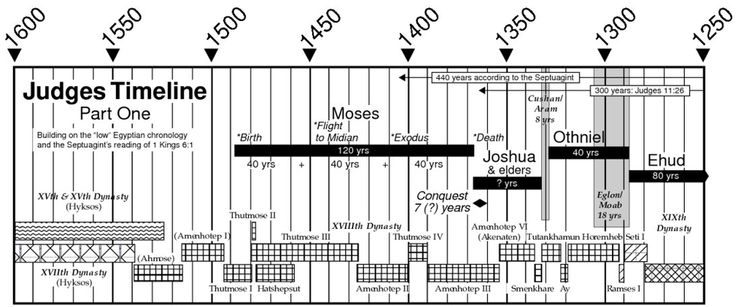
\includegraphics[scale=0.8, angle=90]{07OT-Judges/References/10.Timeline1-Judges}
\caption[Timeline of Judges]{Timeline of Judges}
\label{fig:Timeline of Judges}
\end{center}
\end{figure}



\newpage
\begin{figure}
\begin{center}
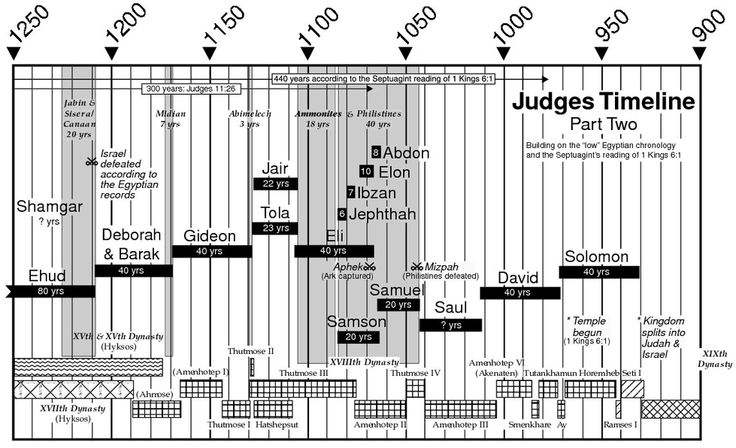
\includegraphics[scale=0.6, angle=90]{07OT-Judges/References/11.Timeline2-Judges}
\caption[Timeline2 of Judges]{Timeline2 of Judges}
\label{fig:Timeline2 of Judges}
\end{center}
\end{figure}


\newpage
\begin{figure}
\begin{center}
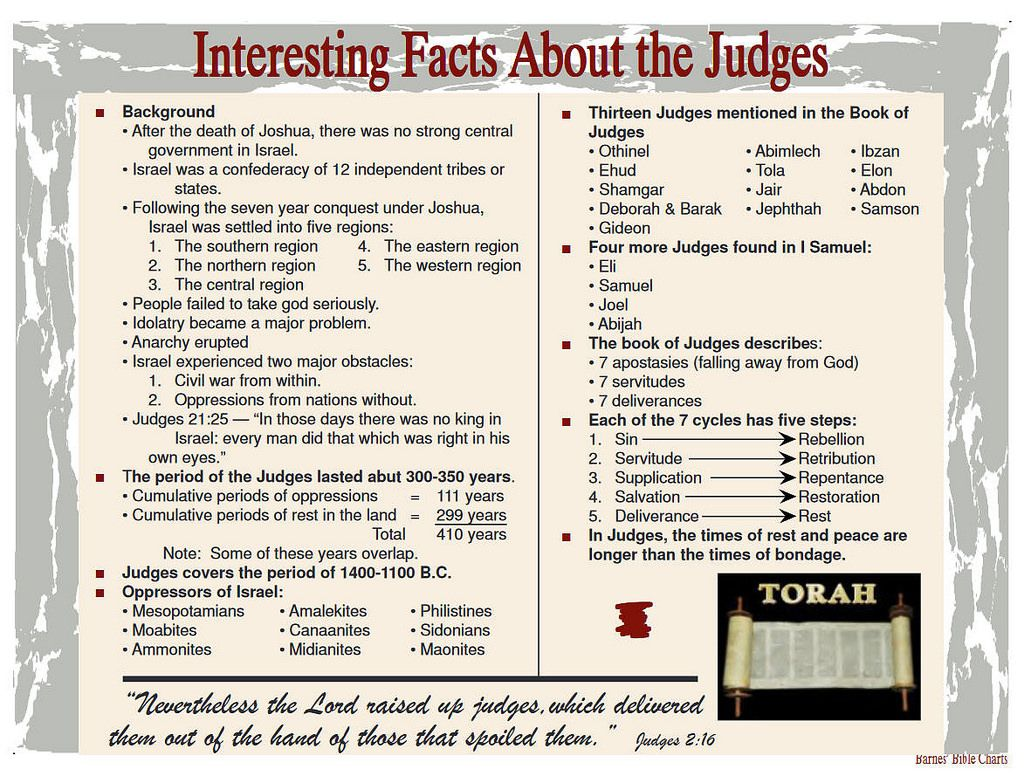
\includegraphics[scale=0.6, angle=90]{07OT-Judges/References/14.InterestingFactsonJudges}
\caption[Interesting Facts about Judges]{Interesting Facts about Judges}
\label{fig:Interesting Facts about Judges}
\end{center}
\end{figure}



\chapter{Judges 1}

\begin{figure}
  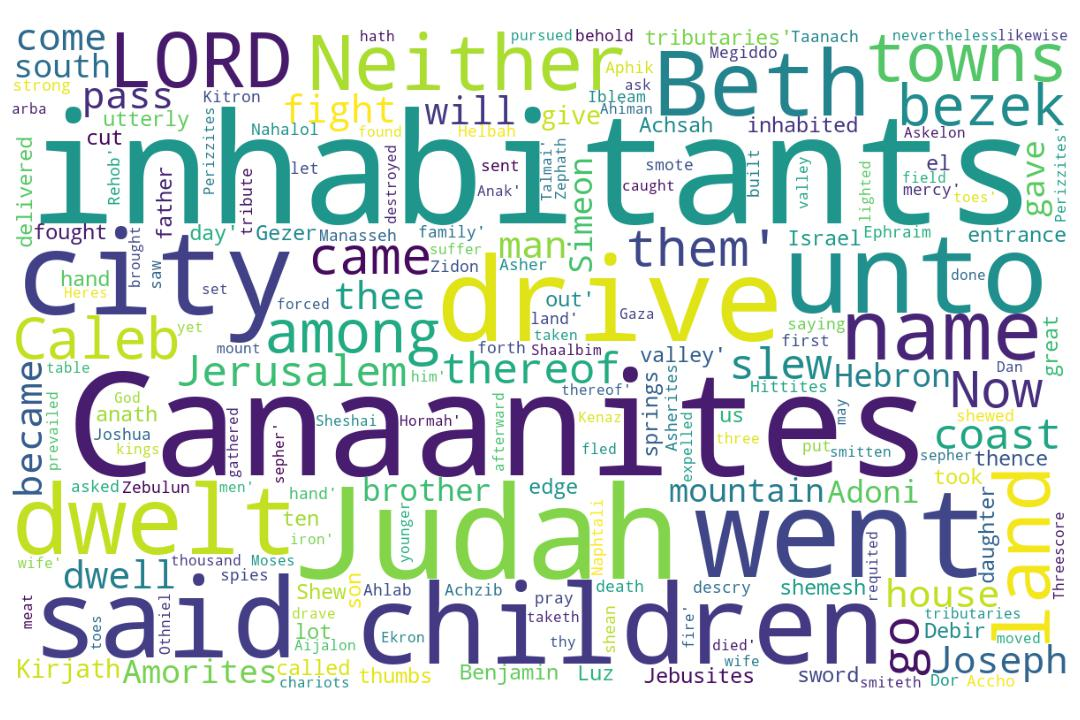
\includegraphics[width=\linewidth]{07OT-Judges/Judges1-WordCloud.jpg}
  \caption{Judges 1 Word Cloud}
  \label{fig:Judges 1 Word Cloud}
\end{figure}


\marginpar{\scriptsize \centering \fcolorbox{bone}{lime}{\textbf{THEYRE BACK}}\\ (Judges 1:1-36) \begin{compactenum}[I.][8]
    \item   A \textbf{Passing}  \index[scripture]{Judges!Jdg 01:01} (Jdg 1:1) 
    \item   The \textbf{Perrizites}  \index[scripture]{Judges!Jdg 01:04} \index[scripture]{Judges!Jdg 01:05} (Jdg 1:4, 5) 
    \item   The  \textbf{Pursuit}  \index[scripture]{Judges!Jdg 01:06} (Jdg 1:6) 
    \item   The  \textbf{Payback}  \index[scripture]{Judges!Jdg 01:07} (Jdg 1:7) 
    \item   The  \textbf{Pyrotechnics}  \index[scripture]{Judges!Jdg 01:08} (Jdg 1:8) 
    \item   The  \textbf{Prominent}  \index[scripture]{Judges!Jdg 01:10} (Jdg 1:10) 
    \item   The  \textbf{Promise}  \index[scripture]{Judges!Jdg 01:12} (Jdg 1:12) 
    \item   A Supposed \textbf{Problem}  \index[scripture]{Judges!Jdg 01:10} \index[scripture]{Judges!Jdg 01:20} (Jdg 1:10, 20) 
\end{compactenum}}

\marginpar{\scriptsize \centering \fcolorbox{bone}{yellow}{\textbf{UNFINISHED BUSINESS}}\\ (Judges 1:1-36) \begin{compactenum}[I.][8]
    \item  The \textbf{Canaanite Focus}  \index[scripture]{Judges!Jdg 01:01} (Jdg 1:1) 
    \item  \textbf{Compromised Faith}  \index[scripture]{Judges!Jdg 01:03}  (Jdg 1:3) 
    \item  \textbf{Casualities Forced}  \index[scripture]{Judges!Jdg 01:04} (Jdg 1:4) 
    \item  \textbf{Cut Feet}  \index[scripture]{Judges!Jdg 01:06-07} (Jdg 1:6-7) 
   \item  A \textbf{City on Fire}  \index[scripture]{Judges!Jdg 01:08} (Jdg 1:14-15) 
   \item  A \textbf{Call of a Female}  \index[scripture]{Judges!Jdg 01:14-15} (Jdg 1:14-15) 
    \item  \textbf{Caleb's Family}  \index[scripture]{Judges!Jdg 01:12} (Jdg 1:12) 
    \item  A \textbf{Call of a Female}  \index[scripture]{Judges!Jdg 01:14-15} (Jdg 1:14-15) 
\end{compactenum}}

\footnote{\textcolor[cmyk]{0.99998,1,0,0}{\hyperlink{TOC}{Return to end of Table of Contents.}}}\footnote{\href{https://audiobible.com/bible/judges_1.html}{\textcolor[cmyk]{0.99998,1,0,0}{Judges 1 Audio}}}\textcolor[cmyk]{0.99998,1,0,0}{Now after the \fcolorbox{bone}{lime}{death of Joshua} it came to pass, that the children of Israel asked the LORD, saying, Who shall go up for us against the Canaanites first, to fight against them?}
[2] \textcolor[cmyk]{0.99998,1,0,0}{And the LORD said, Judah shall go up: behold, I have delivered the land into his hand.}
[3] \textcolor[cmyk]{0.99998,1,0,0}{And Judah said unto Simeon his brother, Come up \fcolorbox{bone}{bone}{with} me into my lot, that we may fight against the Canaanites; and I likewise will go \fcolorbox{bone}{bone}{with} thee into thy lot. So Simeon went \fcolorbox{bone}{bone}{with} him.}
[4] \textcolor[cmyk]{0.99998,1,0,0}{And Judah went up; and the LORD delivered the Canaanites and the \fcolorbox{bone}{lime}{Perizzites} into their hand: and they slew of them in Bezek ten thousand men.}
[5] \textcolor[cmyk]{0.99998,1,0,0}{And they found Adoni-bezek in Bezek: and they fought against him, and they slew the Canaanites and the \fcolorbox{bone}{lime}{Perizzites}.}
[6] \textcolor[cmyk]{0.99998,1,0,0}{But Adoni-bezek fled; and they \fcolorbox{bone}{lime}{pursued} after him, and caught him, and cut off his thumbs and his great toes.}
[7] \textcolor[cmyk]{0.99998,1,0,0}{And Adoni-bezek said, Threescore and ten kings, having their thumbs and their great toes cut off, gathered \emph{their} \emph{meat} under my table: as I have done, so God hath \fcolorbox{bone}{lime}{requited} me. And they brought him to Jerusalem, and there he died.}
[8] \textcolor[cmyk]{0.99998,1,0,0}{Now the children of Judah had fought against Jerusalem, and had taken it, and smitten it \fcolorbox{bone}{bone}{with} the edge \fcolorbox{bone}{bone}{of the} sword, and set the city on \fcolorbox{bone}{lime}{fire}.}\\
\\
\P \textcolor[cmyk]{0.99998,1,0,0}{And afterward the children of Judah went down to fight against the Canaanites, that dwelt in the mountain, and in the south, and in the valley.}
[10] \textcolor[cmyk]{0.99998,1,0,0}{And Judah went against the Canaanites that dwelt in Hebron: (now the name of Hebron before \emph{was} Kirjath-arba:) and they slew \fcolorbox{bone}{lime}{Sheshai}, and \fcolorbox{bone}{lime}{Ahiman}, and \fcolorbox{bone}{lime}{Talmai}.}
[11] \textcolor[cmyk]{0.99998,1,0,0}{And from thence he went against the inhabitants of Debir: and the name of Debir before \emph{was} Kirjath-sepher:}
[12] \textcolor[cmyk]{0.99998,1,0,0}{And Caleb said, He that smiteth Kirjath-sepher, and taketh it, to him \fcolorbox{bone}{lime}{will I give} Achsah my daughter to wife.}
[13] \textcolor[cmyk]{0.99998,1,0,0}{And Othniel the son of Kenaz, Caleb's younger brother, took it: and he gave him Achsah his daughter to wife.}
[14] \textcolor[cmyk]{0.99998,1,0,0}{And it came to pass, when she came \emph{to} \emph{him}, that she moved him to ask of her father a field: and she lighted from off \emph{her} ass; and Caleb said unto her, What wilt thou?}
[15] \textcolor[cmyk]{0.99998,1,0,0}{And she said unto him, Give me a blessing: for thou hast given me a south land; give me also springs of water. And Caleb gave her the upper springs and the nether springs.}\\
\\
\P \textcolor[cmyk]{0.99998,1,0,0}{And the children \fcolorbox{bone}{bone}{of the} Kenite, Moses' father in law, went up out \fcolorbox{bone}{bone}{of the} city of palm trees \fcolorbox{bone}{bone}{with} the children of Judah into the wilderness of Judah, which \emph{lieth} in the south of Arad; and they went and dwelt among the people.}
[17] \textcolor[cmyk]{0.99998,1,0,0}{And Judah went \fcolorbox{bone}{bone}{with} Simeon his brother, and they slew the Canaanites that inhabited Zephath, and utterly destroyed it. And the name \fcolorbox{bone}{bone}{of the} city was called Hormah.}
[18] \textcolor[cmyk]{0.99998,1,0,0}{Also Judah took Gaza \fcolorbox{bone}{bone}{with} the coast thereof, and Askelon \fcolorbox{bone}{bone}{with} the coast thereof, and Ekron \fcolorbox{bone}{bone}{with} the coast thereof.}
[19] \textcolor[cmyk]{0.99998,1,0,0}{And the LORD was \fcolorbox{bone}{bone}{with} Judah; and he drave out \emph{the} \emph{inhabitants} \emph{of} the mountain; but could not drive out the inhabitants \fcolorbox{bone}{bone}{of the} valley, because they had chariots of iron.}
[20] \textcolor[cmyk]{0.99998,1,0,0}{And they gave Hebron unto Caleb, as Moses said: and he expelled thence the three sons of Anak.}
[21] \textcolor[cmyk]{0.99998,1,0,0}{And the children of Benjamin did not drive out the Jebusites that inhabited Jerusalem; but the Jebusites dwell \fcolorbox{bone}{bone}{with} the children of Benjamin in Jerusalem unto this day.}\\
\\
\P \textcolor[cmyk]{0.99998,1,0,0}{And the house of Joseph, they also went up against Beth-el: and the LORD \emph{was} \fcolorbox{bone}{bone}{with} them.}
[23] \textcolor[cmyk]{0.99998,1,0,0}{And the house of Joseph sent to descry Beth-el. (Now the name \fcolorbox{bone}{bone}{of the} city before \emph{was} Luz.)}
[24] \textcolor[cmyk]{0.99998,1,0,0}{And the spies saw a man come forth out \fcolorbox{bone}{bone}{of the} city, and they said unto him, Shew us, we pray thee, the entrance into the city, and we will shew thee mercy.}
[25] \textcolor[cmyk]{0.99998,1,0,0}{And when he shewed them the entrance into the city, they smote the city \fcolorbox{bone}{bone}{with} the edge \fcolorbox{bone}{bone}{of the} sword; but they let go the man and all his family.}
[26] \textcolor[cmyk]{0.99998,1,0,0}{And the man went into the land \fcolorbox{bone}{bone}{of the} Hittites, and built a city, and called the name thereof Luz: which \emph{is} the name thereof unto this day.}\\
\\
\P \textcolor[cmyk]{0.99998,1,0,0}{Neither did Manasseh drive out \emph{the} \emph{inhabitants} \emph{of} Beth-shean and her towns, nor Taanach and her towns, nor the inhabitants of Dor and her towns, nor the inhabitants of Ibleam and her towns, nor the inhabitants of Megiddo and her towns: but the Canaanites would dwell in that land.}
[28] \textcolor[cmyk]{0.99998,1,0,0}{And it came to pass, when Israel was strong, that they put the Canaanites to tribute, and did not utterly drive them out.}\\
\\
\P \textcolor[cmyk]{0.99998,1,0,0}{Neither did Ephraim drive out the Canaanites that dwelt in Gezer; but the Canaanites dwelt in Gezer among them.}\\
\\
\P \textcolor[cmyk]{0.99998,1,0,0}{Neither did Zebulun drive out the inhabitants of Kitron, nor the inhabitants of Nahalol; but the Canaanites dwelt among them, and became tributaries.}
[31] \textcolor[cmyk]{0.99998,1,0,0}{Neither did Asher drive out the inhabitants of Accho, nor the inhabitants of Zidon, nor of Ahlab, nor of Achzib, nor of Helbah, nor of Aphik, nor of Rehob:}
[32] \textcolor[cmyk]{0.99998,1,0,0}{But the Asherites dwelt among the Canaanites, the inhabitants \fcolorbox{bone}{bone}{of the} land: for they did not drive them out.}\\
\\
\P \textcolor[cmyk]{0.99998,1,0,0}{Neither did Naphtali drive out the inhabitants of Beth-shemesh, nor the inhabitants of Beth-anath; but he dwelt among the Canaanites, the inhabitants \fcolorbox{bone}{bone}{of the} land: nevertheless the inhabitants of Beth-shemesh and of Beth-anath became tributaries unto them.}
[34] \textcolor[cmyk]{0.99998,1,0,0}{And the Amorites forced the children of Dan into the mountain: for they would not suffer them to come down to the valley:}
[35] \textcolor[cmyk]{0.99998,1,0,0}{But the Amorites would dwell in mount Heres in Aijalon, and in Shaalbim: yet the hand \fcolorbox{bone}{bone}{of the} house of Joseph prevailed, so that they became tributaries.}
[36] \textcolor[cmyk]{0.99998,1,0,0}{And the coast \fcolorbox{bone}{bone}{of the} Amorites \emph{was} from the going up to Akrabbim, from the rock, and upward.}
\index[NWIV]{33!Judges!Jud 1:1}\index[AWIP]{Now!Judges!Jud 1:1}\index[AWIP]{after!Judges!Jud 1:1}\index[AWIP]{the!Judges!Jud 1:1}\index[AWIP]{the!Judges!Jud 1:1 (2)}\index[AWIP]{the!Judges!Jud 1:1 (3)}\index[AWIP]{the!Judges!Jud 1:1 (4)}\index[AWIP]{death!Judges!Jud 1:1}\index[AWIP]{of!Judges!Jud 1:1}\index[AWIP]{of!Judges!Jud 1:1 (2)}\index[AWIP]{Joshua!Judges!Jud 1:1}\index[AWIP]{it!Judges!Jud 1:1}\index[AWIP]{came!Judges!Jud 1:1}\index[AWIP]{to!Judges!Jud 1:1}\index[AWIP]{to!Judges!Jud 1:1 (2)}\index[AWIP]{pass!Judges!Jud 1:1}\index[AWIP]{that!Judges!Jud 1:1}\index[AWIP]{children!Judges!Jud 1:1}\index[AWIP]{Israel!Judges!Jud 1:1}\index[AWIP]{asked!Judges!Jud 1:1}\index[AWIP]{LORD!Judges!Jud 1:1}\index[AWIP]{saying!Judges!Jud 1:1}\index[AWIP]{Who!Judges!Jud 1:1}\index[AWIP]{shall!Judges!Jud 1:1}\index[AWIP]{go!Judges!Jud 1:1}\index[AWIP]{up!Judges!Jud 1:1}\index[AWIP]{for!Judges!Jud 1:1}\index[AWIP]{us!Judges!Jud 1:1}\index[AWIP]{against!Judges!Jud 1:1}\index[AWIP]{against!Judges!Jud 1:1 (2)}\index[AWIP]{Canaanites!Judges!Jud 1:1}\index[AWIP]{first!Judges!Jud 1:1}\index[AWIP]{fight!Judges!Jud 1:1}\index[AWIP]{them?!Judges!Jud 1:1}

\index[NWIV]{17!Judges!Jud 1:2}\index[AWIP]{And!Judges!Jud 1:2}\index[AWIP]{the!Judges!Jud 1:2}\index[AWIP]{the!Judges!Jud 1:2 (2)}\index[AWIP]{LORD!Judges!Jud 1:2}\index[AWIP]{said!Judges!Jud 1:2}\index[AWIP]{Judah!Judges!Jud 1:2}\index[AWIP]{shall!Judges!Jud 1:2}\index[AWIP]{go!Judges!Jud 1:2}\index[AWIP]{up!Judges!Jud 1:2}\index[AWIP]{behold!Judges!Jud 1:2}\index[AWIP]{I!Judges!Jud 1:2}\index[AWIP]{have!Judges!Jud 1:2}\index[AWIP]{delivered!Judges!Jud 1:2}\index[AWIP]{land!Judges!Jud 1:2}\index[AWIP]{into!Judges!Jud 1:2}\index[AWIP]{his!Judges!Jud 1:2}\index[AWIP]{hand!Judges!Jud 1:2}

\index[NWIV]{36!Judges!Jud 1:3}\index[AWIP]{And!Judges!Jud 1:3}\index[AWIP]{Judah!Judges!Jud 1:3}\index[AWIP]{said!Judges!Jud 1:3}\index[AWIP]{unto!Judges!Jud 1:3}\index[AWIP]{Simeon!Judges!Jud 1:3}\index[AWIP]{Simeon!Judges!Jud 1:3 (2)}\index[AWIP]{his!Judges!Jud 1:3}\index[AWIP]{brother!Judges!Jud 1:3}\index[AWIP]{Come!Judges!Jud 1:3}\index[AWIP]{up!Judges!Jud 1:3}\index[AWIP]{with!Judges!Jud 1:3}\index[AWIP]{with!Judges!Jud 1:3 (2)}\index[AWIP]{with!Judges!Jud 1:3 (3)}\index[AWIP]{me!Judges!Jud 1:3}\index[AWIP]{into!Judges!Jud 1:3}\index[AWIP]{into!Judges!Jud 1:3 (2)}\index[AWIP]{my!Judges!Jud 1:3}\index[AWIP]{lot!Judges!Jud 1:3}\index[AWIP]{lot!Judges!Jud 1:3 (2)}\index[AWIP]{that!Judges!Jud 1:3}\index[AWIP]{we!Judges!Jud 1:3}\index[AWIP]{may!Judges!Jud 1:3}\index[AWIP]{fight!Judges!Jud 1:3}\index[AWIP]{against!Judges!Jud 1:3}\index[AWIP]{the!Judges!Jud 1:3}\index[AWIP]{Canaanites!Judges!Jud 1:3}\index[AWIP]{and!Judges!Jud 1:3}\index[AWIP]{I!Judges!Jud 1:3}\index[AWIP]{likewise!Judges!Jud 1:3}\index[AWIP]{will!Judges!Jud 1:3}\index[AWIP]{go!Judges!Jud 1:3}\index[AWIP]{thee!Judges!Jud 1:3}\index[AWIP]{thy!Judges!Jud 1:3}\index[AWIP]{So!Judges!Jud 1:3}\index[AWIP]{went!Judges!Jud 1:3}\index[AWIP]{him!Judges!Jud 1:3}

\index[NWIV]{26!Judges!Jud 1:4}\index[AWIP]{And!Judges!Jud 1:4}\index[AWIP]{Judah!Judges!Jud 1:4}\index[AWIP]{went!Judges!Jud 1:4}\index[AWIP]{up!Judges!Jud 1:4}\index[AWIP]{and!Judges!Jud 1:4}\index[AWIP]{and!Judges!Jud 1:4 (2)}\index[AWIP]{and!Judges!Jud 1:4 (3)}\index[AWIP]{the!Judges!Jud 1:4}\index[AWIP]{the!Judges!Jud 1:4 (2)}\index[AWIP]{the!Judges!Jud 1:4 (3)}\index[AWIP]{LORD!Judges!Jud 1:4}\index[AWIP]{delivered!Judges!Jud 1:4}\index[AWIP]{Canaanites!Judges!Jud 1:4}\index[AWIP]{Perizzites!Judges!Jud 1:4}\index[AWIP]{into!Judges!Jud 1:4}\index[AWIP]{their!Judges!Jud 1:4}\index[AWIP]{hand!Judges!Jud 1:4}\index[AWIP]{they!Judges!Jud 1:4}\index[AWIP]{slew!Judges!Jud 1:4}\index[AWIP]{of!Judges!Jud 1:4}\index[AWIP]{them!Judges!Jud 1:4}\index[AWIP]{in!Judges!Jud 1:4}\index[AWIP]{Bezek!Judges!Jud 1:4}\index[AWIP]{ten!Judges!Jud 1:4}\index[AWIP]{thousand!Judges!Jud 1:4}\index[AWIP]{men!Judges!Jud 1:4}

\index[NWIV]{19!Judges!Jud 1:5}\index[AWIP]{And!Judges!Jud 1:5}\index[AWIP]{they!Judges!Jud 1:5}\index[AWIP]{they!Judges!Jud 1:5 (2)}\index[AWIP]{they!Judges!Jud 1:5 (3)}\index[AWIP]{found!Judges!Jud 1:5}\index[AWIP]{Adoni-bezek!Judges!Jud 1:5}\index[AWIP]{in!Judges!Jud 1:5}\index[AWIP]{Bezek!Judges!Jud 1:5}\index[AWIP]{and!Judges!Jud 1:5}\index[AWIP]{and!Judges!Jud 1:5 (2)}\index[AWIP]{and!Judges!Jud 1:5 (3)}\index[AWIP]{fought!Judges!Jud 1:5}\index[AWIP]{against!Judges!Jud 1:5}\index[AWIP]{him!Judges!Jud 1:5}\index[AWIP]{slew!Judges!Jud 1:5}\index[AWIP]{the!Judges!Jud 1:5}\index[AWIP]{the!Judges!Jud 1:5 (2)}\index[AWIP]{Canaanites!Judges!Jud 1:5}\index[AWIP]{Perizzites!Judges!Jud 1:5}

\index[NWIV]{20!Judges!Jud 1:6}\index[AWIP]{But!Judges!Jud 1:6}\index[AWIP]{Adoni-bezek!Judges!Jud 1:6}\index[AWIP]{fled!Judges!Jud 1:6}\index[AWIP]{and!Judges!Jud 1:6}\index[AWIP]{and!Judges!Jud 1:6 (2)}\index[AWIP]{and!Judges!Jud 1:6 (3)}\index[AWIP]{and!Judges!Jud 1:6 (4)}\index[AWIP]{they!Judges!Jud 1:6}\index[AWIP]{pursued!Judges!Jud 1:6}\index[AWIP]{after!Judges!Jud 1:6}\index[AWIP]{him!Judges!Jud 1:6}\index[AWIP]{him!Judges!Jud 1:6 (2)}\index[AWIP]{caught!Judges!Jud 1:6}\index[AWIP]{cut!Judges!Jud 1:6}\index[AWIP]{off!Judges!Jud 1:6}\index[AWIP]{his!Judges!Jud 1:6}\index[AWIP]{his!Judges!Jud 1:6 (2)}\index[AWIP]{thumbs!Judges!Jud 1:6}\index[AWIP]{great!Judges!Jud 1:6}\index[AWIP]{toes!Judges!Jud 1:6}

\index[NWIV]{41!Judges!Jud 1:7}\index[AWIP]{And!Judges!Jud 1:7}\index[AWIP]{And!Judges!Jud 1:7 (2)}\index[AWIP]{Adoni-bezek!Judges!Jud 1:7}\index[AWIP]{said!Judges!Jud 1:7}\index[AWIP]{Threescore!Judges!Jud 1:7}\index[AWIP]{and!Judges!Jud 1:7}\index[AWIP]{and!Judges!Jud 1:7 (2)}\index[AWIP]{and!Judges!Jud 1:7 (3)}\index[AWIP]{ten!Judges!Jud 1:7}\index[AWIP]{kings!Judges!Jud 1:7}\index[AWIP]{having!Judges!Jud 1:7}\index[AWIP]{their!Judges!Jud 1:7}\index[AWIP]{their!Judges!Jud 1:7 (2)}\index[AWIP]{thumbs!Judges!Jud 1:7}\index[AWIP]{great!Judges!Jud 1:7}\index[AWIP]{toes!Judges!Jud 1:7}\index[AWIP]{cut!Judges!Jud 1:7}\index[AWIP]{off!Judges!Jud 1:7}\index[AWIP]{gathered!Judges!Jud 1:7}\index[AWIP]{\emph{their}!Judges!Jud 1:7}\index[AWIP]{\emph{meat}!Judges!Jud 1:7}\index[AWIP]{under!Judges!Jud 1:7}\index[AWIP]{my!Judges!Jud 1:7}\index[AWIP]{table!Judges!Jud 1:7}\index[AWIP]{as!Judges!Jud 1:7}\index[AWIP]{I!Judges!Jud 1:7}\index[AWIP]{have!Judges!Jud 1:7}\index[AWIP]{done!Judges!Jud 1:7}\index[AWIP]{so!Judges!Jud 1:7}\index[AWIP]{God!Judges!Jud 1:7}\index[AWIP]{hath!Judges!Jud 1:7}\index[AWIP]{requited!Judges!Jud 1:7}\index[AWIP]{me!Judges!Jud 1:7}\index[AWIP]{they!Judges!Jud 1:7}\index[AWIP]{brought!Judges!Jud 1:7}\index[AWIP]{him!Judges!Jud 1:7}\index[AWIP]{to!Judges!Jud 1:7}\index[AWIP]{Jerusalem!Judges!Jud 1:7}\index[AWIP]{there!Judges!Jud 1:7}\index[AWIP]{he!Judges!Jud 1:7}\index[AWIP]{died!Judges!Jud 1:7}\index[AWIP]{\emph{their}!Judges!Jud 1:7}\index[AWIP]{\emph{meat}!Judges!Jud 1:7}

\index[NWIV]{28!Judges!Jud 1:8}\index[AWIP]{Now!Judges!Jud 1:8}\index[AWIP]{the!Judges!Jud 1:8}\index[AWIP]{the!Judges!Jud 1:8 (2)}\index[AWIP]{the!Judges!Jud 1:8 (3)}\index[AWIP]{the!Judges!Jud 1:8 (4)}\index[AWIP]{children!Judges!Jud 1:8}\index[AWIP]{of!Judges!Jud 1:8}\index[AWIP]{of!Judges!Jud 1:8 (2)}\index[AWIP]{Judah!Judges!Jud 1:8}\index[AWIP]{had!Judges!Jud 1:8}\index[AWIP]{had!Judges!Jud 1:8 (2)}\index[AWIP]{fought!Judges!Jud 1:8}\index[AWIP]{against!Judges!Jud 1:8}\index[AWIP]{Jerusalem!Judges!Jud 1:8}\index[AWIP]{and!Judges!Jud 1:8}\index[AWIP]{and!Judges!Jud 1:8 (2)}\index[AWIP]{and!Judges!Jud 1:8 (3)}\index[AWIP]{taken!Judges!Jud 1:8}\index[AWIP]{it!Judges!Jud 1:8}\index[AWIP]{it!Judges!Jud 1:8 (2)}\index[AWIP]{smitten!Judges!Jud 1:8}\index[AWIP]{with!Judges!Jud 1:8}\index[AWIP]{edge!Judges!Jud 1:8}\index[AWIP]{sword!Judges!Jud 1:8}\index[AWIP]{set!Judges!Jud 1:8}\index[AWIP]{city!Judges!Jud 1:8}\index[AWIP]{on!Judges!Jud 1:8}\index[AWIP]{fire!Judges!Jud 1:8}

\index[NWIV]{26!Judges!Jud 1:9}\index[AWIP]{And!Judges!Jud 1:9}\index[AWIP]{afterward!Judges!Jud 1:9}\index[AWIP]{the!Judges!Jud 1:9}\index[AWIP]{the!Judges!Jud 1:9 (2)}\index[AWIP]{the!Judges!Jud 1:9 (3)}\index[AWIP]{the!Judges!Jud 1:9 (4)}\index[AWIP]{the!Judges!Jud 1:9 (5)}\index[AWIP]{children!Judges!Jud 1:9}\index[AWIP]{of!Judges!Jud 1:9}\index[AWIP]{Judah!Judges!Jud 1:9}\index[AWIP]{went!Judges!Jud 1:9}\index[AWIP]{down!Judges!Jud 1:9}\index[AWIP]{to!Judges!Jud 1:9}\index[AWIP]{fight!Judges!Jud 1:9}\index[AWIP]{against!Judges!Jud 1:9}\index[AWIP]{Canaanites!Judges!Jud 1:9}\index[AWIP]{that!Judges!Jud 1:9}\index[AWIP]{dwelt!Judges!Jud 1:9}\index[AWIP]{in!Judges!Jud 1:9}\index[AWIP]{in!Judges!Jud 1:9 (2)}\index[AWIP]{in!Judges!Jud 1:9 (3)}\index[AWIP]{mountain!Judges!Jud 1:9}\index[AWIP]{and!Judges!Jud 1:9}\index[AWIP]{and!Judges!Jud 1:9 (2)}\index[AWIP]{south!Judges!Jud 1:9}\index[AWIP]{valley!Judges!Jud 1:9}

\index[NWIV]{26!Judges!Jud 1:10}\index[AWIP]{And!Judges!Jud 1:10}\index[AWIP]{Judah!Judges!Jud 1:10}\index[AWIP]{went!Judges!Jud 1:10}\index[AWIP]{against!Judges!Jud 1:10}\index[AWIP]{the!Judges!Jud 1:10}\index[AWIP]{the!Judges!Jud 1:10 (2)}\index[AWIP]{Canaanites!Judges!Jud 1:10}\index[AWIP]{that!Judges!Jud 1:10}\index[AWIP]{dwelt!Judges!Jud 1:10}\index[AWIP]{in!Judges!Jud 1:10}\index[AWIP]{Hebron!Judges!Jud 1:10}\index[AWIP]{Hebron!Judges!Jud 1:10 (2)}\index[AWIP]{(now!Judges!Jud 1:10}\index[AWIP]{name!Judges!Jud 1:10}\index[AWIP]{of!Judges!Jud 1:10}\index[AWIP]{before!Judges!Jud 1:10}\index[AWIP]{\emph{was}!Judges!Jud 1:10}\index[AWIP]{Kirjath-arba)!Judges!Jud 1:10}\index[AWIP]{and!Judges!Jud 1:10}\index[AWIP]{and!Judges!Jud 1:10 (2)}\index[AWIP]{and!Judges!Jud 1:10 (3)}\index[AWIP]{they!Judges!Jud 1:10}\index[AWIP]{slew!Judges!Jud 1:10}\index[AWIP]{Sheshai!Judges!Jud 1:10}\index[AWIP]{Ahiman!Judges!Jud 1:10}\index[AWIP]{Talmai!Judges!Jud 1:10}\index[AWIP]{\emph{was}!Judges!Jud 1:10}

\index[NWIV]{18!Judges!Jud 1:11}\index[AWIP]{And!Judges!Jud 1:11}\index[AWIP]{from!Judges!Jud 1:11}\index[AWIP]{thence!Judges!Jud 1:11}\index[AWIP]{he!Judges!Jud 1:11}\index[AWIP]{went!Judges!Jud 1:11}\index[AWIP]{against!Judges!Jud 1:11}\index[AWIP]{the!Judges!Jud 1:11}\index[AWIP]{the!Judges!Jud 1:11 (2)}\index[AWIP]{inhabitants!Judges!Jud 1:11}\index[AWIP]{of!Judges!Jud 1:11}\index[AWIP]{of!Judges!Jud 1:11 (2)}\index[AWIP]{Debir!Judges!Jud 1:11}\index[AWIP]{Debir!Judges!Jud 1:11 (2)}\index[AWIP]{and!Judges!Jud 1:11}\index[AWIP]{name!Judges!Jud 1:11}\index[AWIP]{before!Judges!Jud 1:11}\index[AWIP]{\emph{was}!Judges!Jud 1:11}\index[AWIP]{Kirjath-sepher!Judges!Jud 1:11}\index[AWIP]{\emph{was}!Judges!Jud 1:11}

\index[NWIV]{20!Judges!Jud 1:12}\index[AWIP]{And!Judges!Jud 1:12}\index[AWIP]{Caleb!Judges!Jud 1:12}\index[AWIP]{said!Judges!Jud 1:12}\index[AWIP]{He!Judges!Jud 1:12}\index[AWIP]{that!Judges!Jud 1:12}\index[AWIP]{smiteth!Judges!Jud 1:12}\index[AWIP]{Kirjath-sepher!Judges!Jud 1:12}\index[AWIP]{and!Judges!Jud 1:12}\index[AWIP]{taketh!Judges!Jud 1:12}\index[AWIP]{it!Judges!Jud 1:12}\index[AWIP]{to!Judges!Jud 1:12}\index[AWIP]{to!Judges!Jud 1:12 (2)}\index[AWIP]{him!Judges!Jud 1:12}\index[AWIP]{will!Judges!Jud 1:12}\index[AWIP]{I!Judges!Jud 1:12}\index[AWIP]{give!Judges!Jud 1:12}\index[AWIP]{Achsah!Judges!Jud 1:12}\index[AWIP]{my!Judges!Jud 1:12}\index[AWIP]{daughter!Judges!Jud 1:12}\index[AWIP]{wife!Judges!Jud 1:12}

\index[NWIV]{20!Judges!Jud 1:13}\index[AWIP]{And!Judges!Jud 1:13}\index[AWIP]{Othniel!Judges!Jud 1:13}\index[AWIP]{the!Judges!Jud 1:13}\index[AWIP]{son!Judges!Jud 1:13}\index[AWIP]{of!Judges!Jud 1:13}\index[AWIP]{Kenaz!Judges!Jud 1:13}\index[AWIP]{Caleb's!Judges!Jud 1:13}\index[AWIP]{younger!Judges!Jud 1:13}\index[AWIP]{brother!Judges!Jud 1:13}\index[AWIP]{took!Judges!Jud 1:13}\index[AWIP]{it!Judges!Jud 1:13}\index[AWIP]{and!Judges!Jud 1:13}\index[AWIP]{he!Judges!Jud 1:13}\index[AWIP]{gave!Judges!Jud 1:13}\index[AWIP]{him!Judges!Jud 1:13}\index[AWIP]{Achsah!Judges!Jud 1:13}\index[AWIP]{his!Judges!Jud 1:13}\index[AWIP]{daughter!Judges!Jud 1:13}\index[AWIP]{to!Judges!Jud 1:13}\index[AWIP]{wife!Judges!Jud 1:13}

\index[NWIV]{36!Judges!Jud 1:14}\index[AWIP]{And!Judges!Jud 1:14}\index[AWIP]{it!Judges!Jud 1:14}\index[AWIP]{came!Judges!Jud 1:14}\index[AWIP]{came!Judges!Jud 1:14 (2)}\index[AWIP]{to!Judges!Jud 1:14}\index[AWIP]{to!Judges!Jud 1:14 (2)}\index[AWIP]{pass!Judges!Jud 1:14}\index[AWIP]{when!Judges!Jud 1:14}\index[AWIP]{she!Judges!Jud 1:14}\index[AWIP]{she!Judges!Jud 1:14 (2)}\index[AWIP]{she!Judges!Jud 1:14 (3)}\index[AWIP]{\emph{to}!Judges!Jud 1:14}\index[AWIP]{\emph{him}!Judges!Jud 1:14}\index[AWIP]{that!Judges!Jud 1:14}\index[AWIP]{moved!Judges!Jud 1:14}\index[AWIP]{him!Judges!Jud 1:14}\index[AWIP]{ask!Judges!Jud 1:14}\index[AWIP]{of!Judges!Jud 1:14}\index[AWIP]{her!Judges!Jud 1:14}\index[AWIP]{her!Judges!Jud 1:14 (2)}\index[AWIP]{father!Judges!Jud 1:14}\index[AWIP]{a!Judges!Jud 1:14}\index[AWIP]{field!Judges!Jud 1:14}\index[AWIP]{and!Judges!Jud 1:14}\index[AWIP]{and!Judges!Jud 1:14 (2)}\index[AWIP]{lighted!Judges!Jud 1:14}\index[AWIP]{from!Judges!Jud 1:14}\index[AWIP]{off!Judges!Jud 1:14}\index[AWIP]{\emph{her}!Judges!Jud 1:14}\index[AWIP]{ass!Judges!Jud 1:14}\index[AWIP]{Caleb!Judges!Jud 1:14}\index[AWIP]{said!Judges!Jud 1:14}\index[AWIP]{unto!Judges!Jud 1:14}\index[AWIP]{What!Judges!Jud 1:14}\index[AWIP]{wilt!Judges!Jud 1:14}\index[AWIP]{thou?!Judges!Jud 1:14}\index[AWIP]{\emph{to}!Judges!Jud 1:14}\index[AWIP]{\emph{him}!Judges!Jud 1:14}\index[AWIP]{\emph{her}!Judges!Jud 1:14}

\index[NWIV]{34!Judges!Jud 1:15}\index[AWIP]{And!Judges!Jud 1:15}\index[AWIP]{And!Judges!Jud 1:15 (2)}\index[AWIP]{she!Judges!Jud 1:15}\index[AWIP]{said!Judges!Jud 1:15}\index[AWIP]{unto!Judges!Jud 1:15}\index[AWIP]{him!Judges!Jud 1:15}\index[AWIP]{Give!Judges!Jud 1:15}\index[AWIP]{me!Judges!Jud 1:15}\index[AWIP]{me!Judges!Jud 1:15 (2)}\index[AWIP]{me!Judges!Jud 1:15 (3)}\index[AWIP]{a!Judges!Jud 1:15}\index[AWIP]{a!Judges!Jud 1:15 (2)}\index[AWIP]{blessing!Judges!Jud 1:15}\index[AWIP]{for!Judges!Jud 1:15}\index[AWIP]{thou!Judges!Jud 1:15}\index[AWIP]{hast!Judges!Jud 1:15}\index[AWIP]{given!Judges!Jud 1:15}\index[AWIP]{south!Judges!Jud 1:15}\index[AWIP]{land!Judges!Jud 1:15}\index[AWIP]{give!Judges!Jud 1:15}\index[AWIP]{also!Judges!Jud 1:15}\index[AWIP]{springs!Judges!Jud 1:15}\index[AWIP]{springs!Judges!Jud 1:15 (2)}\index[AWIP]{springs!Judges!Jud 1:15 (3)}\index[AWIP]{of!Judges!Jud 1:15}\index[AWIP]{water!Judges!Jud 1:15}\index[AWIP]{Caleb!Judges!Jud 1:15}\index[AWIP]{gave!Judges!Jud 1:15}\index[AWIP]{her!Judges!Jud 1:15}\index[AWIP]{the!Judges!Jud 1:15}\index[AWIP]{the!Judges!Jud 1:15 (2)}\index[AWIP]{upper!Judges!Jud 1:15}\index[AWIP]{and!Judges!Jud 1:15}\index[AWIP]{nether!Judges!Jud 1:15}

\index[NWIV]{44!Judges!Jud 1:16}\index[AWIP]{And!Judges!Jud 1:16}\index[AWIP]{the!Judges!Jud 1:16}\index[AWIP]{the!Judges!Jud 1:16 (2)}\index[AWIP]{the!Judges!Jud 1:16 (3)}\index[AWIP]{the!Judges!Jud 1:16 (4)}\index[AWIP]{the!Judges!Jud 1:16 (5)}\index[AWIP]{the!Judges!Jud 1:16 (6)}\index[AWIP]{the!Judges!Jud 1:16 (7)}\index[AWIP]{children!Judges!Jud 1:16}\index[AWIP]{children!Judges!Jud 1:16 (2)}\index[AWIP]{of!Judges!Jud 1:16}\index[AWIP]{of!Judges!Jud 1:16 (2)}\index[AWIP]{of!Judges!Jud 1:16 (3)}\index[AWIP]{of!Judges!Jud 1:16 (4)}\index[AWIP]{of!Judges!Jud 1:16 (5)}\index[AWIP]{of!Judges!Jud 1:16 (6)}\index[AWIP]{Kenite!Judges!Jud 1:16}\index[AWIP]{Moses'!Judges!Jud 1:16}\index[AWIP]{father!Judges!Jud 1:16}\index[AWIP]{in!Judges!Jud 1:16}\index[AWIP]{in!Judges!Jud 1:16 (2)}\index[AWIP]{law!Judges!Jud 1:16}\index[AWIP]{went!Judges!Jud 1:16}\index[AWIP]{went!Judges!Jud 1:16 (2)}\index[AWIP]{up!Judges!Jud 1:16}\index[AWIP]{out!Judges!Jud 1:16}\index[AWIP]{city!Judges!Jud 1:16}\index[AWIP]{palm!Judges!Jud 1:16}\index[AWIP]{trees!Judges!Jud 1:16}\index[AWIP]{with!Judges!Jud 1:16}\index[AWIP]{Judah!Judges!Jud 1:16}\index[AWIP]{Judah!Judges!Jud 1:16 (2)}\index[AWIP]{into!Judges!Jud 1:16}\index[AWIP]{wilderness!Judges!Jud 1:16}\index[AWIP]{which!Judges!Jud 1:16}\index[AWIP]{\emph{lieth}!Judges!Jud 1:16}\index[AWIP]{south!Judges!Jud 1:16}\index[AWIP]{Arad!Judges!Jud 1:16}\index[AWIP]{and!Judges!Jud 1:16}\index[AWIP]{and!Judges!Jud 1:16 (2)}\index[AWIP]{they!Judges!Jud 1:16}\index[AWIP]{dwelt!Judges!Jud 1:16}\index[AWIP]{among!Judges!Jud 1:16}\index[AWIP]{people!Judges!Jud 1:16}\index[AWIP]{\emph{lieth}!Judges!Jud 1:16}

\index[NWIV]{28!Judges!Jud 1:17}\index[AWIP]{And!Judges!Jud 1:17}\index[AWIP]{And!Judges!Jud 1:17 (2)}\index[AWIP]{Judah!Judges!Jud 1:17}\index[AWIP]{went!Judges!Jud 1:17}\index[AWIP]{with!Judges!Jud 1:17}\index[AWIP]{Simeon!Judges!Jud 1:17}\index[AWIP]{his!Judges!Jud 1:17}\index[AWIP]{brother!Judges!Jud 1:17}\index[AWIP]{and!Judges!Jud 1:17}\index[AWIP]{and!Judges!Jud 1:17 (2)}\index[AWIP]{they!Judges!Jud 1:17}\index[AWIP]{slew!Judges!Jud 1:17}\index[AWIP]{the!Judges!Jud 1:17}\index[AWIP]{the!Judges!Jud 1:17 (2)}\index[AWIP]{the!Judges!Jud 1:17 (3)}\index[AWIP]{Canaanites!Judges!Jud 1:17}\index[AWIP]{that!Judges!Jud 1:17}\index[AWIP]{inhabited!Judges!Jud 1:17}\index[AWIP]{Zephath!Judges!Jud 1:17}\index[AWIP]{utterly!Judges!Jud 1:17}\index[AWIP]{destroyed!Judges!Jud 1:17}\index[AWIP]{it!Judges!Jud 1:17}\index[AWIP]{name!Judges!Jud 1:17}\index[AWIP]{of!Judges!Jud 1:17}\index[AWIP]{city!Judges!Jud 1:17}\index[AWIP]{was!Judges!Jud 1:17}\index[AWIP]{called!Judges!Jud 1:17}\index[AWIP]{Hormah!Judges!Jud 1:17}

\index[NWIV]{20!Judges!Jud 1:18}\index[AWIP]{Also!Judges!Jud 1:18}\index[AWIP]{Judah!Judges!Jud 1:18}\index[AWIP]{took!Judges!Jud 1:18}\index[AWIP]{Gaza!Judges!Jud 1:18}\index[AWIP]{with!Judges!Jud 1:18}\index[AWIP]{with!Judges!Jud 1:18 (2)}\index[AWIP]{with!Judges!Jud 1:18 (3)}\index[AWIP]{the!Judges!Jud 1:18}\index[AWIP]{the!Judges!Jud 1:18 (2)}\index[AWIP]{the!Judges!Jud 1:18 (3)}\index[AWIP]{coast!Judges!Jud 1:18}\index[AWIP]{coast!Judges!Jud 1:18 (2)}\index[AWIP]{coast!Judges!Jud 1:18 (3)}\index[AWIP]{thereof!Judges!Jud 1:18}\index[AWIP]{thereof!Judges!Jud 1:18 (2)}\index[AWIP]{thereof!Judges!Jud 1:18 (3)}\index[AWIP]{and!Judges!Jud 1:18}\index[AWIP]{and!Judges!Jud 1:18 (2)}\index[AWIP]{Askelon!Judges!Jud 1:18}\index[AWIP]{Ekron!Judges!Jud 1:18}

\index[NWIV]{31!Judges!Jud 1:19}\index[AWIP]{And!Judges!Jud 1:19}\index[AWIP]{the!Judges!Jud 1:19}\index[AWIP]{the!Judges!Jud 1:19 (2)}\index[AWIP]{the!Judges!Jud 1:19 (3)}\index[AWIP]{the!Judges!Jud 1:19 (4)}\index[AWIP]{LORD!Judges!Jud 1:19}\index[AWIP]{was!Judges!Jud 1:19}\index[AWIP]{with!Judges!Jud 1:19}\index[AWIP]{Judah!Judges!Jud 1:19}\index[AWIP]{and!Judges!Jud 1:19}\index[AWIP]{he!Judges!Jud 1:19}\index[AWIP]{drave!Judges!Jud 1:19}\index[AWIP]{out!Judges!Jud 1:19}\index[AWIP]{out!Judges!Jud 1:19 (2)}\index[AWIP]{\emph{the}!Judges!Jud 1:19}\index[AWIP]{\emph{inhabitants}!Judges!Jud 1:19}\index[AWIP]{\emph{of}!Judges!Jud 1:19}\index[AWIP]{mountain!Judges!Jud 1:19}\index[AWIP]{but!Judges!Jud 1:19}\index[AWIP]{could!Judges!Jud 1:19}\index[AWIP]{not!Judges!Jud 1:19}\index[AWIP]{drive!Judges!Jud 1:19}\index[AWIP]{inhabitants!Judges!Jud 1:19}\index[AWIP]{of!Judges!Jud 1:19}\index[AWIP]{of!Judges!Jud 1:19 (2)}\index[AWIP]{valley!Judges!Jud 1:19}\index[AWIP]{because!Judges!Jud 1:19}\index[AWIP]{they!Judges!Jud 1:19}\index[AWIP]{had!Judges!Jud 1:19}\index[AWIP]{chariots!Judges!Jud 1:19}\index[AWIP]{iron!Judges!Jud 1:19}\index[AWIP]{\emph{the}!Judges!Jud 1:19}\index[AWIP]{\emph{inhabitants}!Judges!Jud 1:19}\index[AWIP]{\emph{of}!Judges!Jud 1:19}

\index[NWIV]{18!Judges!Jud 1:20}\index[AWIP]{And!Judges!Jud 1:20}\index[AWIP]{they!Judges!Jud 1:20}\index[AWIP]{gave!Judges!Jud 1:20}\index[AWIP]{Hebron!Judges!Jud 1:20}\index[AWIP]{unto!Judges!Jud 1:20}\index[AWIP]{Caleb!Judges!Jud 1:20}\index[AWIP]{as!Judges!Jud 1:20}\index[AWIP]{Moses!Judges!Jud 1:20}\index[AWIP]{said!Judges!Jud 1:20}\index[AWIP]{and!Judges!Jud 1:20}\index[AWIP]{he!Judges!Jud 1:20}\index[AWIP]{expelled!Judges!Jud 1:20}\index[AWIP]{thence!Judges!Jud 1:20}\index[AWIP]{the!Judges!Jud 1:20}\index[AWIP]{three!Judges!Jud 1:20}\index[AWIP]{sons!Judges!Jud 1:20}\index[AWIP]{of!Judges!Jud 1:20}\index[AWIP]{Anak!Judges!Jud 1:20}

\index[NWIV]{28!Judges!Jud 1:21}\index[AWIP]{And!Judges!Jud 1:21}\index[AWIP]{the!Judges!Jud 1:21}\index[AWIP]{the!Judges!Jud 1:21 (2)}\index[AWIP]{the!Judges!Jud 1:21 (3)}\index[AWIP]{the!Judges!Jud 1:21 (4)}\index[AWIP]{children!Judges!Jud 1:21}\index[AWIP]{children!Judges!Jud 1:21 (2)}\index[AWIP]{of!Judges!Jud 1:21}\index[AWIP]{of!Judges!Jud 1:21 (2)}\index[AWIP]{Benjamin!Judges!Jud 1:21}\index[AWIP]{Benjamin!Judges!Jud 1:21 (2)}\index[AWIP]{did!Judges!Jud 1:21}\index[AWIP]{not!Judges!Jud 1:21}\index[AWIP]{drive!Judges!Jud 1:21}\index[AWIP]{out!Judges!Jud 1:21}\index[AWIP]{Jebusites!Judges!Jud 1:21}\index[AWIP]{Jebusites!Judges!Jud 1:21 (2)}\index[AWIP]{that!Judges!Jud 1:21}\index[AWIP]{inhabited!Judges!Jud 1:21}\index[AWIP]{Jerusalem!Judges!Jud 1:21}\index[AWIP]{Jerusalem!Judges!Jud 1:21 (2)}\index[AWIP]{but!Judges!Jud 1:21}\index[AWIP]{dwell!Judges!Jud 1:21}\index[AWIP]{with!Judges!Jud 1:21}\index[AWIP]{in!Judges!Jud 1:21}\index[AWIP]{unto!Judges!Jud 1:21}\index[AWIP]{this!Judges!Jud 1:21}\index[AWIP]{day!Judges!Jud 1:21}

\index[NWIV]{17!Judges!Jud 1:22}\index[AWIP]{And!Judges!Jud 1:22}\index[AWIP]{the!Judges!Jud 1:22}\index[AWIP]{the!Judges!Jud 1:22 (2)}\index[AWIP]{house!Judges!Jud 1:22}\index[AWIP]{of!Judges!Jud 1:22}\index[AWIP]{Joseph!Judges!Jud 1:22}\index[AWIP]{they!Judges!Jud 1:22}\index[AWIP]{also!Judges!Jud 1:22}\index[AWIP]{went!Judges!Jud 1:22}\index[AWIP]{up!Judges!Jud 1:22}\index[AWIP]{against!Judges!Jud 1:22}\index[AWIP]{Beth-el!Judges!Jud 1:22}\index[AWIP]{and!Judges!Jud 1:22}\index[AWIP]{LORD!Judges!Jud 1:22}\index[AWIP]{\emph{was}!Judges!Jud 1:22}\index[AWIP]{with!Judges!Jud 1:22}\index[AWIP]{them!Judges!Jud 1:22}\index[AWIP]{\emph{was}!Judges!Jud 1:22}

\index[NWIV]{18!Judges!Jud 1:23}\index[AWIP]{And!Judges!Jud 1:23}\index[AWIP]{the!Judges!Jud 1:23}\index[AWIP]{the!Judges!Jud 1:23 (2)}\index[AWIP]{the!Judges!Jud 1:23 (3)}\index[AWIP]{house!Judges!Jud 1:23}\index[AWIP]{of!Judges!Jud 1:23}\index[AWIP]{of!Judges!Jud 1:23 (2)}\index[AWIP]{Joseph!Judges!Jud 1:23}\index[AWIP]{sent!Judges!Jud 1:23}\index[AWIP]{to!Judges!Jud 1:23}\index[AWIP]{descry!Judges!Jud 1:23}\index[AWIP]{Beth-el!Judges!Jud 1:23}\index[AWIP]{(Now!Judges!Jud 1:23}\index[AWIP]{name!Judges!Jud 1:23}\index[AWIP]{city!Judges!Jud 1:23}\index[AWIP]{before!Judges!Jud 1:23}\index[AWIP]{\emph{was}!Judges!Jud 1:23}\index[AWIP]{Luz)!Judges!Jud 1:23}\index[AWIP]{\emph{was}!Judges!Jud 1:23}

\index[NWIV]{33!Judges!Jud 1:24}\index[AWIP]{And!Judges!Jud 1:24}\index[AWIP]{the!Judges!Jud 1:24}\index[AWIP]{the!Judges!Jud 1:24 (2)}\index[AWIP]{the!Judges!Jud 1:24 (3)}\index[AWIP]{the!Judges!Jud 1:24 (4)}\index[AWIP]{spies!Judges!Jud 1:24}\index[AWIP]{saw!Judges!Jud 1:24}\index[AWIP]{a!Judges!Jud 1:24}\index[AWIP]{man!Judges!Jud 1:24}\index[AWIP]{come!Judges!Jud 1:24}\index[AWIP]{forth!Judges!Jud 1:24}\index[AWIP]{out!Judges!Jud 1:24}\index[AWIP]{of!Judges!Jud 1:24}\index[AWIP]{city!Judges!Jud 1:24}\index[AWIP]{city!Judges!Jud 1:24 (2)}\index[AWIP]{and!Judges!Jud 1:24}\index[AWIP]{and!Judges!Jud 1:24 (2)}\index[AWIP]{they!Judges!Jud 1:24}\index[AWIP]{said!Judges!Jud 1:24}\index[AWIP]{unto!Judges!Jud 1:24}\index[AWIP]{him!Judges!Jud 1:24}\index[AWIP]{Shew!Judges!Jud 1:24}\index[AWIP]{us!Judges!Jud 1:24}\index[AWIP]{we!Judges!Jud 1:24}\index[AWIP]{we!Judges!Jud 1:24 (2)}\index[AWIP]{pray!Judges!Jud 1:24}\index[AWIP]{thee!Judges!Jud 1:24}\index[AWIP]{thee!Judges!Jud 1:24 (2)}\index[AWIP]{entrance!Judges!Jud 1:24}\index[AWIP]{into!Judges!Jud 1:24}\index[AWIP]{will!Judges!Jud 1:24}\index[AWIP]{shew!Judges!Jud 1:24}\index[AWIP]{mercy!Judges!Jud 1:24}

\index[NWIV]{30!Judges!Jud 1:25}\index[AWIP]{And!Judges!Jud 1:25}\index[AWIP]{when!Judges!Jud 1:25}\index[AWIP]{he!Judges!Jud 1:25}\index[AWIP]{shewed!Judges!Jud 1:25}\index[AWIP]{them!Judges!Jud 1:25}\index[AWIP]{the!Judges!Jud 1:25}\index[AWIP]{the!Judges!Jud 1:25 (2)}\index[AWIP]{the!Judges!Jud 1:25 (3)}\index[AWIP]{the!Judges!Jud 1:25 (4)}\index[AWIP]{the!Judges!Jud 1:25 (5)}\index[AWIP]{the!Judges!Jud 1:25 (6)}\index[AWIP]{entrance!Judges!Jud 1:25}\index[AWIP]{into!Judges!Jud 1:25}\index[AWIP]{city!Judges!Jud 1:25}\index[AWIP]{city!Judges!Jud 1:25 (2)}\index[AWIP]{they!Judges!Jud 1:25}\index[AWIP]{they!Judges!Jud 1:25 (2)}\index[AWIP]{smote!Judges!Jud 1:25}\index[AWIP]{with!Judges!Jud 1:25}\index[AWIP]{edge!Judges!Jud 1:25}\index[AWIP]{of!Judges!Jud 1:25}\index[AWIP]{sword!Judges!Jud 1:25}\index[AWIP]{but!Judges!Jud 1:25}\index[AWIP]{let!Judges!Jud 1:25}\index[AWIP]{go!Judges!Jud 1:25}\index[AWIP]{man!Judges!Jud 1:25}\index[AWIP]{and!Judges!Jud 1:25}\index[AWIP]{all!Judges!Jud 1:25}\index[AWIP]{his!Judges!Jud 1:25}\index[AWIP]{family!Judges!Jud 1:25}

\index[NWIV]{28!Judges!Jud 1:26}\index[AWIP]{And!Judges!Jud 1:26}\index[AWIP]{the!Judges!Jud 1:26}\index[AWIP]{the!Judges!Jud 1:26 (2)}\index[AWIP]{the!Judges!Jud 1:26 (3)}\index[AWIP]{the!Judges!Jud 1:26 (4)}\index[AWIP]{the!Judges!Jud 1:26 (5)}\index[AWIP]{man!Judges!Jud 1:26}\index[AWIP]{went!Judges!Jud 1:26}\index[AWIP]{into!Judges!Jud 1:26}\index[AWIP]{land!Judges!Jud 1:26}\index[AWIP]{of!Judges!Jud 1:26}\index[AWIP]{Hittites!Judges!Jud 1:26}\index[AWIP]{and!Judges!Jud 1:26}\index[AWIP]{and!Judges!Jud 1:26 (2)}\index[AWIP]{built!Judges!Jud 1:26}\index[AWIP]{a!Judges!Jud 1:26}\index[AWIP]{city!Judges!Jud 1:26}\index[AWIP]{called!Judges!Jud 1:26}\index[AWIP]{name!Judges!Jud 1:26}\index[AWIP]{name!Judges!Jud 1:26 (2)}\index[AWIP]{thereof!Judges!Jud 1:26}\index[AWIP]{thereof!Judges!Jud 1:26 (2)}\index[AWIP]{Luz!Judges!Jud 1:26}\index[AWIP]{which!Judges!Jud 1:26}\index[AWIP]{\emph{is}!Judges!Jud 1:26}\index[AWIP]{unto!Judges!Jud 1:26}\index[AWIP]{this!Judges!Jud 1:26}\index[AWIP]{day!Judges!Jud 1:26}\index[AWIP]{\emph{is}!Judges!Jud 1:26}

\index[NWIV]{49!Judges!Jud 1:27}\index[AWIP]{Neither!Judges!Jud 1:27}\index[AWIP]{did!Judges!Jud 1:27}\index[AWIP]{Manasseh!Judges!Jud 1:27}\index[AWIP]{drive!Judges!Jud 1:27}\index[AWIP]{out!Judges!Jud 1:27}\index[AWIP]{\emph{the}!Judges!Jud 1:27}\index[AWIP]{\emph{inhabitants}!Judges!Jud 1:27}\index[AWIP]{\emph{of}!Judges!Jud 1:27}\index[AWIP]{Beth-shean!Judges!Jud 1:27}\index[AWIP]{and!Judges!Jud 1:27}\index[AWIP]{and!Judges!Jud 1:27 (2)}\index[AWIP]{and!Judges!Jud 1:27 (3)}\index[AWIP]{and!Judges!Jud 1:27 (4)}\index[AWIP]{and!Judges!Jud 1:27 (5)}\index[AWIP]{her!Judges!Jud 1:27}\index[AWIP]{her!Judges!Jud 1:27 (2)}\index[AWIP]{her!Judges!Jud 1:27 (3)}\index[AWIP]{her!Judges!Jud 1:27 (4)}\index[AWIP]{her!Judges!Jud 1:27 (5)}\index[AWIP]{towns!Judges!Jud 1:27}\index[AWIP]{towns!Judges!Jud 1:27 (2)}\index[AWIP]{towns!Judges!Jud 1:27 (3)}\index[AWIP]{towns!Judges!Jud 1:27 (4)}\index[AWIP]{towns!Judges!Jud 1:27 (5)}\index[AWIP]{nor!Judges!Jud 1:27}\index[AWIP]{nor!Judges!Jud 1:27 (2)}\index[AWIP]{nor!Judges!Jud 1:27 (3)}\index[AWIP]{nor!Judges!Jud 1:27 (4)}\index[AWIP]{Taanach!Judges!Jud 1:27}\index[AWIP]{the!Judges!Jud 1:27}\index[AWIP]{the!Judges!Jud 1:27 (2)}\index[AWIP]{the!Judges!Jud 1:27 (3)}\index[AWIP]{the!Judges!Jud 1:27 (4)}\index[AWIP]{inhabitants!Judges!Jud 1:27}\index[AWIP]{inhabitants!Judges!Jud 1:27 (2)}\index[AWIP]{inhabitants!Judges!Jud 1:27 (3)}\index[AWIP]{of!Judges!Jud 1:27}\index[AWIP]{of!Judges!Jud 1:27 (2)}\index[AWIP]{of!Judges!Jud 1:27 (3)}\index[AWIP]{Dor!Judges!Jud 1:27}\index[AWIP]{Ibleam!Judges!Jud 1:27}\index[AWIP]{Megiddo!Judges!Jud 1:27}\index[AWIP]{but!Judges!Jud 1:27}\index[AWIP]{Canaanites!Judges!Jud 1:27}\index[AWIP]{would!Judges!Jud 1:27}\index[AWIP]{dwell!Judges!Jud 1:27}\index[AWIP]{in!Judges!Jud 1:27}\index[AWIP]{that!Judges!Jud 1:27}\index[AWIP]{land!Judges!Jud 1:27}\index[AWIP]{\emph{the}!Judges!Jud 1:27}\index[AWIP]{\emph{inhabitants}!Judges!Jud 1:27}\index[AWIP]{\emph{of}!Judges!Jud 1:27}

\index[NWIV]{23!Judges!Jud 1:28}\index[AWIP]{And!Judges!Jud 1:28}\index[AWIP]{it!Judges!Jud 1:28}\index[AWIP]{came!Judges!Jud 1:28}\index[AWIP]{to!Judges!Jud 1:28}\index[AWIP]{to!Judges!Jud 1:28 (2)}\index[AWIP]{pass!Judges!Jud 1:28}\index[AWIP]{when!Judges!Jud 1:28}\index[AWIP]{Israel!Judges!Jud 1:28}\index[AWIP]{was!Judges!Jud 1:28}\index[AWIP]{strong!Judges!Jud 1:28}\index[AWIP]{that!Judges!Jud 1:28}\index[AWIP]{they!Judges!Jud 1:28}\index[AWIP]{put!Judges!Jud 1:28}\index[AWIP]{the!Judges!Jud 1:28}\index[AWIP]{Canaanites!Judges!Jud 1:28}\index[AWIP]{tribute!Judges!Jud 1:28}\index[AWIP]{and!Judges!Jud 1:28}\index[AWIP]{did!Judges!Jud 1:28}\index[AWIP]{not!Judges!Jud 1:28}\index[AWIP]{utterly!Judges!Jud 1:28}\index[AWIP]{drive!Judges!Jud 1:28}\index[AWIP]{them!Judges!Jud 1:28}\index[AWIP]{out!Judges!Jud 1:28}

\index[NWIV]{19!Judges!Jud 1:29}\index[AWIP]{Neither!Judges!Jud 1:29}\index[AWIP]{did!Judges!Jud 1:29}\index[AWIP]{Ephraim!Judges!Jud 1:29}\index[AWIP]{drive!Judges!Jud 1:29}\index[AWIP]{out!Judges!Jud 1:29}\index[AWIP]{the!Judges!Jud 1:29}\index[AWIP]{the!Judges!Jud 1:29 (2)}\index[AWIP]{Canaanites!Judges!Jud 1:29}\index[AWIP]{Canaanites!Judges!Jud 1:29 (2)}\index[AWIP]{that!Judges!Jud 1:29}\index[AWIP]{dwelt!Judges!Jud 1:29}\index[AWIP]{dwelt!Judges!Jud 1:29 (2)}\index[AWIP]{in!Judges!Jud 1:29}\index[AWIP]{in!Judges!Jud 1:29 (2)}\index[AWIP]{Gezer!Judges!Jud 1:29}\index[AWIP]{Gezer!Judges!Jud 1:29 (2)}\index[AWIP]{but!Judges!Jud 1:29}\index[AWIP]{among!Judges!Jud 1:29}\index[AWIP]{them!Judges!Jud 1:29}

\index[NWIV]{23!Judges!Jud 1:30}\index[AWIP]{Neither!Judges!Jud 1:30}\index[AWIP]{did!Judges!Jud 1:30}\index[AWIP]{Zebulun!Judges!Jud 1:30}\index[AWIP]{drive!Judges!Jud 1:30}\index[AWIP]{out!Judges!Jud 1:30}\index[AWIP]{the!Judges!Jud 1:30}\index[AWIP]{the!Judges!Jud 1:30 (2)}\index[AWIP]{the!Judges!Jud 1:30 (3)}\index[AWIP]{inhabitants!Judges!Jud 1:30}\index[AWIP]{inhabitants!Judges!Jud 1:30 (2)}\index[AWIP]{of!Judges!Jud 1:30}\index[AWIP]{of!Judges!Jud 1:30 (2)}\index[AWIP]{Kitron!Judges!Jud 1:30}\index[AWIP]{nor!Judges!Jud 1:30}\index[AWIP]{Nahalol!Judges!Jud 1:30}\index[AWIP]{but!Judges!Jud 1:30}\index[AWIP]{Canaanites!Judges!Jud 1:30}\index[AWIP]{dwelt!Judges!Jud 1:30}\index[AWIP]{among!Judges!Jud 1:30}\index[AWIP]{them!Judges!Jud 1:30}\index[AWIP]{and!Judges!Jud 1:30}\index[AWIP]{became!Judges!Jud 1:30}\index[AWIP]{tributaries!Judges!Jud 1:30}

\index[NWIV]{29!Judges!Jud 1:31}\index[AWIP]{Neither!Judges!Jud 1:31}\index[AWIP]{did!Judges!Jud 1:31}\index[AWIP]{Asher!Judges!Jud 1:31}\index[AWIP]{drive!Judges!Jud 1:31}\index[AWIP]{out!Judges!Jud 1:31}\index[AWIP]{the!Judges!Jud 1:31}\index[AWIP]{the!Judges!Jud 1:31 (2)}\index[AWIP]{inhabitants!Judges!Jud 1:31}\index[AWIP]{inhabitants!Judges!Jud 1:31 (2)}\index[AWIP]{of!Judges!Jud 1:31}\index[AWIP]{of!Judges!Jud 1:31 (2)}\index[AWIP]{of!Judges!Jud 1:31 (3)}\index[AWIP]{of!Judges!Jud 1:31 (4)}\index[AWIP]{of!Judges!Jud 1:31 (5)}\index[AWIP]{of!Judges!Jud 1:31 (6)}\index[AWIP]{of!Judges!Jud 1:31 (7)}\index[AWIP]{Accho!Judges!Jud 1:31}\index[AWIP]{nor!Judges!Jud 1:31}\index[AWIP]{nor!Judges!Jud 1:31 (2)}\index[AWIP]{nor!Judges!Jud 1:31 (3)}\index[AWIP]{nor!Judges!Jud 1:31 (4)}\index[AWIP]{nor!Judges!Jud 1:31 (5)}\index[AWIP]{nor!Judges!Jud 1:31 (6)}\index[AWIP]{Zidon!Judges!Jud 1:31}\index[AWIP]{Ahlab!Judges!Jud 1:31}\index[AWIP]{Achzib!Judges!Jud 1:31}\index[AWIP]{Helbah!Judges!Jud 1:31}\index[AWIP]{Aphik!Judges!Jud 1:31}\index[AWIP]{Rehob!Judges!Jud 1:31}

\index[NWIV]{19!Judges!Jud 1:32}\index[AWIP]{But!Judges!Jud 1:32}\index[AWIP]{the!Judges!Jud 1:32}\index[AWIP]{the!Judges!Jud 1:32 (2)}\index[AWIP]{the!Judges!Jud 1:32 (3)}\index[AWIP]{the!Judges!Jud 1:32 (4)}\index[AWIP]{Asherites!Judges!Jud 1:32}\index[AWIP]{dwelt!Judges!Jud 1:32}\index[AWIP]{among!Judges!Jud 1:32}\index[AWIP]{Canaanites!Judges!Jud 1:32}\index[AWIP]{inhabitants!Judges!Jud 1:32}\index[AWIP]{of!Judges!Jud 1:32}\index[AWIP]{land!Judges!Jud 1:32}\index[AWIP]{for!Judges!Jud 1:32}\index[AWIP]{they!Judges!Jud 1:32}\index[AWIP]{did!Judges!Jud 1:32}\index[AWIP]{not!Judges!Jud 1:32}\index[AWIP]{drive!Judges!Jud 1:32}\index[AWIP]{them!Judges!Jud 1:32}\index[AWIP]{out!Judges!Jud 1:32}

\index[NWIV]{37!Judges!Jud 1:33}\index[AWIP]{Neither!Judges!Jud 1:33}\index[AWIP]{did!Judges!Jud 1:33}\index[AWIP]{Naphtali!Judges!Jud 1:33}\index[AWIP]{drive!Judges!Jud 1:33}\index[AWIP]{out!Judges!Jud 1:33}\index[AWIP]{the!Judges!Jud 1:33}\index[AWIP]{the!Judges!Jud 1:33 (2)}\index[AWIP]{the!Judges!Jud 1:33 (3)}\index[AWIP]{the!Judges!Jud 1:33 (4)}\index[AWIP]{the!Judges!Jud 1:33 (5)}\index[AWIP]{the!Judges!Jud 1:33 (6)}\index[AWIP]{inhabitants!Judges!Jud 1:33}\index[AWIP]{inhabitants!Judges!Jud 1:33 (2)}\index[AWIP]{inhabitants!Judges!Jud 1:33 (3)}\index[AWIP]{inhabitants!Judges!Jud 1:33 (4)}\index[AWIP]{of!Judges!Jud 1:33}\index[AWIP]{of!Judges!Jud 1:33 (2)}\index[AWIP]{of!Judges!Jud 1:33 (3)}\index[AWIP]{of!Judges!Jud 1:33 (4)}\index[AWIP]{of!Judges!Jud 1:33 (5)}\index[AWIP]{Beth-shemesh!Judges!Jud 1:33}\index[AWIP]{Beth-shemesh!Judges!Jud 1:33 (2)}\index[AWIP]{nor!Judges!Jud 1:33}\index[AWIP]{Beth-anath!Judges!Jud 1:33}\index[AWIP]{Beth-anath!Judges!Jud 1:33 (2)}\index[AWIP]{but!Judges!Jud 1:33}\index[AWIP]{he!Judges!Jud 1:33}\index[AWIP]{dwelt!Judges!Jud 1:33}\index[AWIP]{among!Judges!Jud 1:33}\index[AWIP]{Canaanites!Judges!Jud 1:33}\index[AWIP]{land!Judges!Jud 1:33}\index[AWIP]{nevertheless!Judges!Jud 1:33}\index[AWIP]{and!Judges!Jud 1:33}\index[AWIP]{became!Judges!Jud 1:33}\index[AWIP]{tributaries!Judges!Jud 1:33}\index[AWIP]{unto!Judges!Jud 1:33}\index[AWIP]{them!Judges!Jud 1:33}

\index[NWIV]{23!Judges!Jud 1:34}\index[AWIP]{And!Judges!Jud 1:34}\index[AWIP]{the!Judges!Jud 1:34}\index[AWIP]{the!Judges!Jud 1:34 (2)}\index[AWIP]{the!Judges!Jud 1:34 (3)}\index[AWIP]{the!Judges!Jud 1:34 (4)}\index[AWIP]{Amorites!Judges!Jud 1:34}\index[AWIP]{forced!Judges!Jud 1:34}\index[AWIP]{children!Judges!Jud 1:34}\index[AWIP]{of!Judges!Jud 1:34}\index[AWIP]{Dan!Judges!Jud 1:34}\index[AWIP]{into!Judges!Jud 1:34}\index[AWIP]{mountain!Judges!Jud 1:34}\index[AWIP]{for!Judges!Jud 1:34}\index[AWIP]{they!Judges!Jud 1:34}\index[AWIP]{would!Judges!Jud 1:34}\index[AWIP]{not!Judges!Jud 1:34}\index[AWIP]{suffer!Judges!Jud 1:34}\index[AWIP]{them!Judges!Jud 1:34}\index[AWIP]{to!Judges!Jud 1:34}\index[AWIP]{to!Judges!Jud 1:34 (2)}\index[AWIP]{come!Judges!Jud 1:34}\index[AWIP]{down!Judges!Jud 1:34}\index[AWIP]{valley!Judges!Jud 1:34}

\index[NWIV]{27!Judges!Jud 1:35}\index[AWIP]{But!Judges!Jud 1:35}\index[AWIP]{the!Judges!Jud 1:35}\index[AWIP]{the!Judges!Jud 1:35 (2)}\index[AWIP]{the!Judges!Jud 1:35 (3)}\index[AWIP]{Amorites!Judges!Jud 1:35}\index[AWIP]{would!Judges!Jud 1:35}\index[AWIP]{dwell!Judges!Jud 1:35}\index[AWIP]{in!Judges!Jud 1:35}\index[AWIP]{in!Judges!Jud 1:35 (2)}\index[AWIP]{in!Judges!Jud 1:35 (3)}\index[AWIP]{mount!Judges!Jud 1:35}\index[AWIP]{Heres!Judges!Jud 1:35}\index[AWIP]{Aijalon!Judges!Jud 1:35}\index[AWIP]{and!Judges!Jud 1:35}\index[AWIP]{Shaalbim!Judges!Jud 1:35}\index[AWIP]{yet!Judges!Jud 1:35}\index[AWIP]{hand!Judges!Jud 1:35}\index[AWIP]{of!Judges!Jud 1:35}\index[AWIP]{of!Judges!Jud 1:35 (2)}\index[AWIP]{house!Judges!Jud 1:35}\index[AWIP]{Joseph!Judges!Jud 1:35}\index[AWIP]{prevailed!Judges!Jud 1:35}\index[AWIP]{so!Judges!Jud 1:35}\index[AWIP]{that!Judges!Jud 1:35}\index[AWIP]{they!Judges!Jud 1:35}\index[AWIP]{became!Judges!Jud 1:35}\index[AWIP]{tributaries!Judges!Jud 1:35}

\index[NWIV]{18!Judges!Jud 1:36}\index[AWIP]{And!Judges!Jud 1:36}\index[AWIP]{the!Judges!Jud 1:36}\index[AWIP]{the!Judges!Jud 1:36 (2)}\index[AWIP]{the!Judges!Jud 1:36 (3)}\index[AWIP]{the!Judges!Jud 1:36 (4)}\index[AWIP]{coast!Judges!Jud 1:36}\index[AWIP]{of!Judges!Jud 1:36}\index[AWIP]{Amorites!Judges!Jud 1:36}\index[AWIP]{\emph{was}!Judges!Jud 1:36}\index[AWIP]{from!Judges!Jud 1:36}\index[AWIP]{from!Judges!Jud 1:36 (2)}\index[AWIP]{going!Judges!Jud 1:36}\index[AWIP]{up!Judges!Jud 1:36}\index[AWIP]{to!Judges!Jud 1:36}\index[AWIP]{Akrabbim!Judges!Jud 1:36}\index[AWIP]{rock!Judges!Jud 1:36}\index[AWIP]{and!Judges!Jud 1:36}\index[AWIP]{upward!Judges!Jud 1:36}\index[AWIP]{\emph{was}!Judges!Jud 1:36}


\section{Judges 1 Outlines}

\subsection{My Outlines}

\subsubsection{They're Back  $\hdots$}
\index[speaker]{Keith Anthony!Judges 01 (They're Back  $\hdots$)}
\index[series]{Judges (Keith Anthony)!Judges 01 (They're Back  $\hdots$)}
\index[date]{2018/03/15!Judges 01 (They're Back  $\hdots$) (Keith Anthony)}
\begin{compactenum}[I.][8]
    \item   A \textbf{Passing}  \index[scripture]{Judges!Jdg 01:01} (Jdg 1:1) 
    \item   The \textbf{Perrizites}  \index[scripture]{Judges!Jdg 01:04} \index[scripture]{Judges!Jdg 01:05} (Jdg 1:4, 5) 
    \item   The  \textbf{Pursuit}  \index[scripture]{Judges!Jdg 01:06} (Jdg 1:6) 
    \item   The  \textbf{Payback}  \index[scripture]{Judges!Jdg 01:07} (Jdg 1:7) 
    \item   The  \textbf{Pyrotechnics}  \index[scripture]{Judges!Jdg 01:08} (Jdg 1:8) 
    \item   The  \textbf{Prominent}  \index[scripture]{Judges!Jdg 01:10} (Jdg 1:10) 
    \item   The  \textbf{Promise}  \index[scripture]{Judges!Jdg 01:12} (Jdg 1:12) 
    \item   A Supposed \textbf{Problem}  \index[scripture]{Judges!Jdg 01:10} \index[scripture]{Judges!Jdg 01:20} (Jdg 1:10, 20) -- two possible answers (1) one event with two descriptions or (2) the giants came back after Joshua 15. I go with explanation 1.
\end{compactenum}


\subsubsection{Unfinished Business}
\index[speaker]{Keith Anthony!Judges 01 (Unfinished Business)}
\index[series]{Judges (Keith Anthony)!Judges 01 (Unfinished Business)}
\index[date]{2020/03/14!Judges 01 (Unfinished Business) (Keith Anthony)} \begin{compactenum}[I.][8]
    \item  The \textbf{Canaanite Focus}  \index[scripture]{Judges!Jdg 01:01} (Jdg 1:1) 
    \item  \textbf{Compromised Faith}  \index[scripture]{Judges!Jdg 01:03}  (Jdg 1:3) 
    \item  \textbf{Casualities Forced}  \index[scripture]{Judges!Jdg 01:04} (Jdg 1:4) 
    \item  \textbf{Cut Feet}  \index[scripture]{Judges!Jdg 01:06-07} (Jdg 1:6-7) 
   \item  A \textbf{City on Fire}  \index[scripture]{Judges!Jdg 01:08} (Jdg 1:14-15) 
   \item  A \textbf{Call of a Female}  \index[scripture]{Judges!Jdg 01:14-15} (Jdg 1:14-15) 
    \item  \textbf{Caleb's Family}  \index[scripture]{Judges!Jdg 01:12} (Jdg 1:12) 
    \item  A \textbf{Call of a Female}  \index[scripture]{Judges!Jdg 01:14-15} (Jdg 1:14-15) 
\end{compactenum}


\subsection{Outlines from Others}
\section{Judges 1 Comments}

\subsection{Numeric Nuggets}
\textbf{13: } The phrase ``of the'' is used 13 times in the chapter.
\subsection{Judges 1 Repeated Phrases}


%%%%%%%%%%
%%%%%%%%%%
\normalsize
 
\begin{center}
\begin{longtable}{|p{3.0in}|p{0.5in}|}
\caption[Judges 1 Repeated Phrases]{Judges 1 Repeated Phrases}\label{table:Repeated Phrases Judges 1} \\
\hline \multicolumn{1}{|c|}{\textbf{Phrase}} & \multicolumn{1}{c|}{\textbf{Frequency}} \\ \hline 
\endfirsthead
 
\multicolumn{2}{c}
{{\bfseries \tablename\ \thetable{} -- continued from previous page}} \\  
\hline \multicolumn{1}{|c|}{\textbf{Phrase}} & \multicolumn{1}{c|}{\textbf{Frequency}} \\ \hline 
\endhead
 
\hline \multicolumn{2}{c}{{ }} \\ \hline
\endfoot 
the Canaanites & 14\\ \hline 
the inhabitants & 14\\ \hline 
the inhabitants of & 14\\ \hline 
inhabitants of & 14\\ \hline 
of the & 13\\ \hline 
And the & 11\\ \hline 
the children & 8\\ \hline 
the children of & 8\\ \hline 
children of & 8\\ \hline 
and they & 8\\ \hline 
the city & 8\\ \hline 
with the & 7\\ \hline 
drive out & 7\\ \hline 
and the & 6\\ \hline 
the name & 6\\ \hline 
drive out the & 6\\ \hline 
out the & 6\\ \hline 
nor the & 6\\ \hline 
nor the inhabitants & 6\\ \hline 
nor the inhabitants of & 6\\ \hline 
the LORD & 5\\ \hline 
against the & 5\\ \hline 
into the & 5\\ \hline 
Neither did & 5\\ \hline 
and her & 5\\ \hline 
and her towns & 5\\ \hline 
her towns & 5\\ \hline 
nor of & 5\\ \hline 
against the Canaanites & 4\\ \hline 
the land & 4\\ \hline 
And Judah & 4\\ \hline 
said unto & 4\\ \hline 
Judah went & 4\\ \hline 
and they slew & 4\\ \hline 
they slew & 4\\ \hline 
of Judah & 4\\ \hline 
the Canaanites that & 4\\ \hline 
Canaanites that & 4\\ \hline 
dwelt in & 4\\ \hline 
in the & 4\\ \hline 
the name of & 4\\ \hline 
name of & 4\\ \hline 
of the city & 4\\ \hline 
dwelt among & 4\\ \hline 
the coast & 4\\ \hline 
drive out the inhabitants & 4\\ \hline 
drive out the inhabitants of & 4\\ \hline 
out the inhabitants & 4\\ \hline 
out the inhabitants of & 4\\ \hline 
but the & 4\\ \hline 
and her towns nor & 4\\ \hline 
her towns nor & 4\\ \hline 
towns nor & 4\\ \hline 
it came & 3\\ \hline 
it came to & 3\\ \hline 
it came to pass & 3\\ \hline 
came to & 3\\ \hline 
came to pass & 3\\ \hline 
to pass & 3\\ \hline 
fight against & 3\\ \hline 
the Canaanites and & 3\\ \hline 
Canaanites and & 3\\ \hline 
And Judah went & 3\\ \hline 
went up & 3\\ \hline 
And they & 3\\ \hline 
him and & 3\\ \hline 
the children of Judah & 3\\ \hline 
children of Judah & 3\\ \hline 
the Canaanites that dwelt & 3\\ \hline 
the Canaanites that dwelt in & 3\\ \hline 
Canaanites that dwelt & 3\\ \hline 
Canaanites that dwelt in & 3\\ \hline 
that dwelt & 3\\ \hline 
that dwelt in & 3\\ \hline 
the mountain & 3\\ \hline 
and in & 3\\ \hline 
the valley & 3\\ \hline 
before \emph{was} & 3\\ \hline 
and he & 3\\ \hline 
dwelt among the & 3\\ \hline 
among the & 3\\ \hline 
with the coast & 3\\ \hline 
with the coast thereof & 3\\ \hline 
the coast thereof & 3\\ \hline 
coast thereof & 3\\ \hline 
not drive & 3\\ \hline 
the inhabitants of the & 3\\ \hline 
inhabitants of the & 3\\ \hline 
did not & 3\\ \hline 
the house & 3\\ \hline 
the house of & 3\\ \hline 
the house of Joseph & 3\\ \hline 
house of & 3\\ \hline 
house of Joseph & 3\\ \hline 
of Joseph & 3\\ \hline 
city and & 3\\ \hline 
and her towns nor the & 3\\ \hline 
and her towns nor the inhabitants & 3\\ \hline 
and her towns nor the inhabitants of & 3\\ \hline 
her towns nor the & 3\\ \hline 
her towns nor the inhabitants & 3\\ \hline 
her towns nor the inhabitants of & 3\\ \hline 
towns nor the & 3\\ \hline 
towns nor the inhabitants & 3\\ \hline 
towns nor the inhabitants of & 3\\ \hline 
but the Canaanites & 3\\ \hline 
became tributaries & 3\\ \hline 
the Amorites & 3\\ \hline 
\end{longtable}
\end{center}



%%%%%%%%%%
%%%%%%%%%%



\section{Judges 1 Statistics}

%%%%%%%%%%%%%%%%%%%%%%%%%%%
%%%%% Word Statistics
%%%%%%%%%%%%%%%%%%%%%%%%%%


\normalsize



\subsection{Chapter Word Statistics}


%%%%%%%%%%
%%%%%%%%%%
 
\begin{center}
\begin{longtable}{l|c|c|c|c}
\caption[Stats for Judges 1]{Stats for Judges 1} \label{table:Stats for Judges 1} \\ 
\hline \multicolumn{1}{|c|}{\textbf{Verse(s)}} & \multicolumn{1}{|c|}{\textbf{Count}} & \multicolumn{1}{|c|}{\textbf{Unique}} & \multicolumn{1}{|c|}{\textbf{Italics}} & \multicolumn{1}{|c|}{\textbf{Uniq Italic}}  \\ \hline 
\endfirsthead
 
\multicolumn{5}{c}
{{\bfseries \tablename\ \thetable{} -- continued from previous page}} \\  
\hline \multicolumn{1}{|c|}{\textbf{Verse(s)}} & \multicolumn{1}{|c|}{\textbf{Count}} & \multicolumn{1}{|c|}{\textbf{Unique}} & \multicolumn{1}{|c|}{\textbf{Italics}} & \multicolumn{1}{|c|}{\textbf{Uniq Italic}}  \\ \hline 
\endhead
 
\hline \multicolumn{5}{|r|}{{Continued if needed}} \\ \hline
\endfoot 
1 & 33 & 27 & 0 & 0\\ \hline
2 & 17 & 16 & 0 & 0\\ \hline
3 & 36 & 31 & 0 & 0\\ \hline
4 & 26 & 22 & 0 & 0\\ \hline
5 & 19 & 14 & 0 & 0\\ \hline
6 & 20 & 15 & 0 & 0\\ \hline
7 & 41 & 37 & 2 & 2\\ \hline
8 & 28 & 20 & 0 & 0\\ \hline
9 & 26 & 19 & 0 & 0\\ \hline
10 & 26 & 22 & 1 & 1\\ \hline
11 & 18 & 15 & 1 & 1\\ \hline
12 & 20 & 19 & 0 & 0\\ \hline
13 & 20 & 20 & 0 & 0\\ \hline
14 & 36 & 30 & 3 & 3\\ \hline
15 & 34 & 27 & 0 & 0\\ \hline
16 & 44 & 28 & 1 & 1\\ \hline
17 & 28 & 24 & 0 & 0\\ \hline
18 & 20 & 11 & 0 & 0\\ \hline
19 & 31 & 26 & 3 & 3\\ \hline
20 & 18 & 18 & 0 & 0\\ \hline
21 & 28 & 20 & 0 & 0\\ \hline
22 & 17 & 16 & 1 & 1\\ \hline
23 & 18 & 15 & 1 & 1\\ \hline
24 & 33 & 26 & 0 & 0\\ \hline
25 & 30 & 23 & 0 & 0\\ \hline
26 & 28 & 21 & 1 & 1\\ \hline
27 & 49 & 27 & 3 & 3\\ \hline
28 & 23 & 22 & 0 & 0\\ \hline
29 & 19 & 14 & 0 & 0\\ \hline
30 & 23 & 19 & 0 & 0\\ \hline
31 & 29 & 16 & 0 & 0\\ \hline
32 & 19 & 16 & 0 & 0\\ \hline
33 & 37 & 23 & 0 & 0\\ \hline
34 & 23 & 19 & 0 & 0\\ \hline
35 & 27 & 22 & 0 & 0\\ \hline
36 & 18 & 14 & 1 & 1\\ \hline
\hline \hline
Total & 962 & 283 & 18 & 11



\end{longtable}
\end{center}

%%%%%%%%%%
%%%%%%%%%%
 
\subsection{Words by Frequency}

\begin{center}
\begin{longtable}{l|r}
\caption[Word Frequencies in Judges 1]{Word Frequencies in Judges 1} \label{table:WordsIn-Judges-1} \\ 
\hline \multicolumn{1}{|c|}{\textbf{Word}} & \multicolumn{1}{c|}{\textbf{Frequency}} \\ \hline 
\endfirsthead
 
\multicolumn{2}{c}
{{\bfseries \tablename\ \thetable{} -- continued from previous page}} \\ 
\hline \multicolumn{1}{|c|}{\textbf{Word}} & \multicolumn{1}{c|}{\textbf{Frequency}} \\ \hline 
\endhead
 
\hline \multicolumn{2}{|r|}{{Continued if needed}} \\ \hline
\endfoot
 
\hline \hline
\endlastfoot
the & 103 \\ \hline
of & 52 \\ \hline
and & 52 \\ \hline
And & 28 \\ \hline
they & 19 \\ \hline
to & 15 \\ \hline
in & 15 \\ \hline
Canaanites & 14 \\ \hline
inhabitants & 14 \\ \hline
with & 13 \\ \hline
that & 12 \\ \hline
out & 12 \\ \hline
nor & 12 \\ \hline
Judah & 11 \\ \hline
them & 10 \\ \hline
went & 10 \\ \hline
him & 10 \\ \hline
against & 9 \\ \hline
into & 9 \\ \hline
city & 9 \\ \hline
drive & 9 \\ \hline
it & 8 \\ \hline
children & 8 \\ \hline
said & 8 \\ \hline
unto & 8 \\ \hline
dwelt & 8 \\ \hline
her & 8 \\ \hline
did & 8 \\ \hline
up & 7 \\ \hline
his & 7 \\ \hline
he & 7 \\ \hline
but & 7 \\ \hline
land & 6 \\ \hline
name & 6 \\ \hline
LORD & 5 \\ \hline
me & 5 \\ \hline
\emph{was} & 5 \\ \hline
a & 5 \\ \hline
among & 5 \\ \hline
thereof & 5 \\ \hline
not & 5 \\ \hline
Neither & 5 \\ \hline
towns & 5 \\ \hline
came & 4 \\ \hline
go & 4 \\ \hline
for & 4 \\ \hline
I & 4 \\ \hline
slew & 4 \\ \hline
Jerusalem & 4 \\ \hline
from & 4 \\ \hline
Caleb & 4 \\ \hline
she & 4 \\ \hline
coast & 4 \\ \hline
Now & 3 \\ \hline
pass & 3 \\ \hline
fight & 3 \\ \hline
hand & 3 \\ \hline
Simeon & 3 \\ \hline
brother & 3 \\ \hline
my & 3 \\ \hline
we & 3 \\ \hline
will & 3 \\ \hline
thee & 3 \\ \hline
their & 3 \\ \hline
Adoni-bezek & 3 \\ \hline
But & 3 \\ \hline
off & 3 \\ \hline
had & 3 \\ \hline
mountain & 3 \\ \hline
south & 3 \\ \hline
valley & 3 \\ \hline
Hebron & 3 \\ \hline
before & 3 \\ \hline
gave & 3 \\ \hline
when & 3 \\ \hline
springs & 3 \\ \hline
was & 3 \\ \hline
dwell & 3 \\ \hline
house & 3 \\ \hline
Joseph & 3 \\ \hline
man & 3 \\ \hline
would & 3 \\ \hline
became & 3 \\ \hline
tributaries & 3 \\ \hline
Amorites & 3 \\ \hline
after & 2 \\ \hline
Israel & 2 \\ \hline
shall & 2 \\ \hline
us & 2 \\ \hline
have & 2 \\ \hline
delivered & 2 \\ \hline
lot & 2 \\ \hline
Perizzites & 2 \\ \hline
Bezek & 2 \\ \hline
ten & 2 \\ \hline
fought & 2 \\ \hline
cut & 2 \\ \hline
thumbs & 2 \\ \hline
great & 2 \\ \hline
toes & 2 \\ \hline
as & 2 \\ \hline
so & 2 \\ \hline
edge & 2 \\ \hline
sword & 2 \\ \hline
down & 2 \\ \hline
thence & 2 \\ \hline
Debir & 2 \\ \hline
Kirjath-sepher & 2 \\ \hline
give & 2 \\ \hline
Achsah & 2 \\ \hline
daughter & 2 \\ \hline
wife & 2 \\ \hline
took & 2 \\ \hline
father & 2 \\ \hline
thou & 2 \\ \hline
also & 2 \\ \hline
which & 2 \\ \hline
inhabited & 2 \\ \hline
utterly & 2 \\ \hline
called & 2 \\ \hline
\emph{the} & 2 \\ \hline
\emph{inhabitants} & 2 \\ \hline
\emph{of} & 2 \\ \hline
Benjamin & 2 \\ \hline
Jebusites & 2 \\ \hline
this & 2 \\ \hline
day & 2 \\ \hline
Beth-el & 2 \\ \hline
Luz & 2 \\ \hline
come & 2 \\ \hline
entrance & 2 \\ \hline
Gezer & 2 \\ \hline
Beth-shemesh & 2 \\ \hline
Beth-anath & 2 \\ \hline
death & 1 \\ \hline
Joshua & 1 \\ \hline
asked & 1 \\ \hline
saying & 1 \\ \hline
Who & 1 \\ \hline
first & 1 \\ \hline
behold & 1 \\ \hline
Come & 1 \\ \hline
may & 1 \\ \hline
likewise & 1 \\ \hline
thy & 1 \\ \hline
So & 1 \\ \hline
thousand & 1 \\ \hline
men & 1 \\ \hline
found & 1 \\ \hline
fled & 1 \\ \hline
pursued & 1 \\ \hline
caught & 1 \\ \hline
Threescore & 1 \\ \hline
kings & 1 \\ \hline
having & 1 \\ \hline
gathered & 1 \\ \hline
\emph{their} & 1 \\ \hline
\emph{meat} & 1 \\ \hline
under & 1 \\ \hline
table & 1 \\ \hline
done & 1 \\ \hline
God & 1 \\ \hline
hath & 1 \\ \hline
requited & 1 \\ \hline
brought & 1 \\ \hline
there & 1 \\ \hline
died & 1 \\ \hline
taken & 1 \\ \hline
smitten & 1 \\ \hline
set & 1 \\ \hline
on & 1 \\ \hline
fire & 1 \\ \hline
afterward & 1 \\ \hline
now & 1 \\ \hline
Kirjath-arba & 1 \\ \hline
Sheshai & 1 \\ \hline
Ahiman & 1 \\ \hline
Talmai & 1 \\ \hline
He & 1 \\ \hline
smiteth & 1 \\ \hline
taketh & 1 \\ \hline
Othniel & 1 \\ \hline
son & 1 \\ \hline
Kenaz & 1 \\ \hline
Caleb's & 1 \\ \hline
younger & 1 \\ \hline
\emph{to} & 1 \\ \hline
\emph{him} & 1 \\ \hline
moved & 1 \\ \hline
ask & 1 \\ \hline
field & 1 \\ \hline
lighted & 1 \\ \hline
\emph{her} & 1 \\ \hline
ass & 1 \\ \hline
What & 1 \\ \hline
wilt & 1 \\ \hline
Give & 1 \\ \hline
blessing & 1 \\ \hline
hast & 1 \\ \hline
given & 1 \\ \hline
water & 1 \\ \hline
upper & 1 \\ \hline
nether & 1 \\ \hline
Kenite & 1 \\ \hline
Moses' & 1 \\ \hline
law & 1 \\ \hline
palm & 1 \\ \hline
trees & 1 \\ \hline
wilderness & 1 \\ \hline
\emph{lieth} & 1 \\ \hline
Arad & 1 \\ \hline
people & 1 \\ \hline
Zephath & 1 \\ \hline
destroyed & 1 \\ \hline
Hormah & 1 \\ \hline
Also & 1 \\ \hline
Gaza & 1 \\ \hline
Askelon & 1 \\ \hline
Ekron & 1 \\ \hline
drave & 1 \\ \hline
could & 1 \\ \hline
because & 1 \\ \hline
chariots & 1 \\ \hline
iron & 1 \\ \hline
Moses & 1 \\ \hline
expelled & 1 \\ \hline
three & 1 \\ \hline
sons & 1 \\ \hline
Anak & 1 \\ \hline
sent & 1 \\ \hline
descry & 1 \\ \hline
spies & 1 \\ \hline
saw & 1 \\ \hline
forth & 1 \\ \hline
Shew & 1 \\ \hline
pray & 1 \\ \hline
shew & 1 \\ \hline
mercy & 1 \\ \hline
shewed & 1 \\ \hline
smote & 1 \\ \hline
let & 1 \\ \hline
all & 1 \\ \hline
family & 1 \\ \hline
Hittites & 1 \\ \hline
built & 1 \\ \hline
\emph{is} & 1 \\ \hline
Manasseh & 1 \\ \hline
Beth-shean & 1 \\ \hline
Taanach & 1 \\ \hline
Dor & 1 \\ \hline
Ibleam & 1 \\ \hline
Megiddo & 1 \\ \hline
strong & 1 \\ \hline
put & 1 \\ \hline
tribute & 1 \\ \hline
Ephraim & 1 \\ \hline
Zebulun & 1 \\ \hline
Kitron & 1 \\ \hline
Nahalol & 1 \\ \hline
Asher & 1 \\ \hline
Accho & 1 \\ \hline
Zidon & 1 \\ \hline
Ahlab & 1 \\ \hline
Achzib & 1 \\ \hline
Helbah & 1 \\ \hline
Aphik & 1 \\ \hline
Rehob & 1 \\ \hline
Asherites & 1 \\ \hline
Naphtali & 1 \\ \hline
nevertheless & 1 \\ \hline
forced & 1 \\ \hline
Dan & 1 \\ \hline
suffer & 1 \\ \hline
mount & 1 \\ \hline
Heres & 1 \\ \hline
Aijalon & 1 \\ \hline
Shaalbim & 1 \\ \hline
yet & 1 \\ \hline
prevailed & 1 \\ \hline
going & 1 \\ \hline
Akrabbim & 1 \\ \hline
rock & 1 \\ \hline
upward & 1 \\ \hline
\end{longtable}
\end{center}



\normalsize



\subsection{Words Alphabetically}

\begin{center}
\begin{longtable}{l|r}
\caption[Word Alphabetically in Judges 1]{Word Alphabetically in Judges 1} \label{table:WordsIn-Judges-1} \\ 
\hline \multicolumn{1}{|c|}{\textbf{Word}} & \multicolumn{1}{c|}{\textbf{Frequency}} \\ \hline 
\endfirsthead
 
\multicolumn{2}{c}
{{\bfseries \tablename\ \thetable{} -- continued from previous page}} \\ 
\hline \multicolumn{1}{|c|}{\textbf{Word}} & \multicolumn{1}{c|}{\textbf{Frequency}} \\ \hline 
\endhead
 
\hline \multicolumn{2}{|r|}{{Continued if needed}} \\ \hline
\endfoot
 
\hline \hline
\endlastfoot
Accho & 1 \\ \hline
Achsah & 2 \\ \hline
Achzib & 1 \\ \hline
Adoni-bezek & 3 \\ \hline
Ahiman & 1 \\ \hline
Ahlab & 1 \\ \hline
Aijalon & 1 \\ \hline
Akrabbim & 1 \\ \hline
Also & 1 \\ \hline
Amorites & 3 \\ \hline
Anak & 1 \\ \hline
And & 28 \\ \hline
Aphik & 1 \\ \hline
Arad & 1 \\ \hline
Asher & 1 \\ \hline
Asherites & 1 \\ \hline
Askelon & 1 \\ \hline
Benjamin & 2 \\ \hline
Beth-anath & 2 \\ \hline
Beth-el & 2 \\ \hline
Beth-shean & 1 \\ \hline
Beth-shemesh & 2 \\ \hline
Bezek & 2 \\ \hline
But & 3 \\ \hline
Caleb & 4 \\ \hline
Caleb's & 1 \\ \hline
Canaanites & 14 \\ \hline
Come & 1 \\ \hline
Dan & 1 \\ \hline
Debir & 2 \\ \hline
Dor & 1 \\ \hline
Ekron & 1 \\ \hline
Ephraim & 1 \\ \hline
Gaza & 1 \\ \hline
Gezer & 2 \\ \hline
Give & 1 \\ \hline
God & 1 \\ \hline
He & 1 \\ \hline
Hebron & 3 \\ \hline
Helbah & 1 \\ \hline
Heres & 1 \\ \hline
Hittites & 1 \\ \hline
Hormah & 1 \\ \hline
I & 4 \\ \hline
Ibleam & 1 \\ \hline
Israel & 2 \\ \hline
Jebusites & 2 \\ \hline
Jerusalem & 4 \\ \hline
Joseph & 3 \\ \hline
Joshua & 1 \\ \hline
Judah & 11 \\ \hline
Kenaz & 1 \\ \hline
Kenite & 1 \\ \hline
Kirjath-arba & 1 \\ \hline
Kirjath-sepher & 2 \\ \hline
Kitron & 1 \\ \hline
LORD & 5 \\ \hline
Luz & 2 \\ \hline
Manasseh & 1 \\ \hline
Megiddo & 1 \\ \hline
Moses & 1 \\ \hline
Moses' & 1 \\ \hline
Nahalol & 1 \\ \hline
Naphtali & 1 \\ \hline
Neither & 5 \\ \hline
Now & 3 \\ \hline
Othniel & 1 \\ \hline
Perizzites & 2 \\ \hline
Rehob & 1 \\ \hline
Shaalbim & 1 \\ \hline
Sheshai & 1 \\ \hline
Shew & 1 \\ \hline
Simeon & 3 \\ \hline
So & 1 \\ \hline
Taanach & 1 \\ \hline
Talmai & 1 \\ \hline
Threescore & 1 \\ \hline
What & 1 \\ \hline
Who & 1 \\ \hline
Zebulun & 1 \\ \hline
Zephath & 1 \\ \hline
Zidon & 1 \\ \hline
\emph{her} & 1 \\ \hline
\emph{him} & 1 \\ \hline
\emph{inhabitants} & 2 \\ \hline
\emph{is} & 1 \\ \hline
\emph{lieth} & 1 \\ \hline
\emph{meat} & 1 \\ \hline
\emph{of} & 2 \\ \hline
\emph{their} & 1 \\ \hline
\emph{the} & 2 \\ \hline
\emph{to} & 1 \\ \hline
\emph{was} & 5 \\ \hline
a & 5 \\ \hline
after & 2 \\ \hline
afterward & 1 \\ \hline
against & 9 \\ \hline
all & 1 \\ \hline
also & 2 \\ \hline
among & 5 \\ \hline
and & 52 \\ \hline
as & 2 \\ \hline
ask & 1 \\ \hline
asked & 1 \\ \hline
ass & 1 \\ \hline
became & 3 \\ \hline
because & 1 \\ \hline
before & 3 \\ \hline
behold & 1 \\ \hline
blessing & 1 \\ \hline
brother & 3 \\ \hline
brought & 1 \\ \hline
built & 1 \\ \hline
but & 7 \\ \hline
called & 2 \\ \hline
came & 4 \\ \hline
caught & 1 \\ \hline
chariots & 1 \\ \hline
children & 8 \\ \hline
city & 9 \\ \hline
coast & 4 \\ \hline
come & 2 \\ \hline
could & 1 \\ \hline
cut & 2 \\ \hline
daughter & 2 \\ \hline
day & 2 \\ \hline
death & 1 \\ \hline
delivered & 2 \\ \hline
descry & 1 \\ \hline
destroyed & 1 \\ \hline
did & 8 \\ \hline
died & 1 \\ \hline
done & 1 \\ \hline
down & 2 \\ \hline
drave & 1 \\ \hline
drive & 9 \\ \hline
dwell & 3 \\ \hline
dwelt & 8 \\ \hline
edge & 2 \\ \hline
entrance & 2 \\ \hline
expelled & 1 \\ \hline
family & 1 \\ \hline
father & 2 \\ \hline
field & 1 \\ \hline
fight & 3 \\ \hline
fire & 1 \\ \hline
first & 1 \\ \hline
fled & 1 \\ \hline
for & 4 \\ \hline
forced & 1 \\ \hline
forth & 1 \\ \hline
fought & 2 \\ \hline
found & 1 \\ \hline
from & 4 \\ \hline
gathered & 1 \\ \hline
gave & 3 \\ \hline
give & 2 \\ \hline
given & 1 \\ \hline
go & 4 \\ \hline
going & 1 \\ \hline
great & 2 \\ \hline
had & 3 \\ \hline
hand & 3 \\ \hline
hast & 1 \\ \hline
hath & 1 \\ \hline
have & 2 \\ \hline
having & 1 \\ \hline
he & 7 \\ \hline
her & 8 \\ \hline
him & 10 \\ \hline
his & 7 \\ \hline
house & 3 \\ \hline
in & 15 \\ \hline
inhabitants & 14 \\ \hline
inhabited & 2 \\ \hline
into & 9 \\ \hline
iron & 1 \\ \hline
it & 8 \\ \hline
kings & 1 \\ \hline
land & 6 \\ \hline
law & 1 \\ \hline
let & 1 \\ \hline
lighted & 1 \\ \hline
likewise & 1 \\ \hline
lot & 2 \\ \hline
man & 3 \\ \hline
may & 1 \\ \hline
me & 5 \\ \hline
men & 1 \\ \hline
mercy & 1 \\ \hline
mount & 1 \\ \hline
mountain & 3 \\ \hline
moved & 1 \\ \hline
my & 3 \\ \hline
name & 6 \\ \hline
nether & 1 \\ \hline
nevertheless & 1 \\ \hline
nor & 12 \\ \hline
not & 5 \\ \hline
now & 1 \\ \hline
of & 52 \\ \hline
off & 3 \\ \hline
on & 1 \\ \hline
out & 12 \\ \hline
palm & 1 \\ \hline
pass & 3 \\ \hline
people & 1 \\ \hline
pray & 1 \\ \hline
prevailed & 1 \\ \hline
pursued & 1 \\ \hline
put & 1 \\ \hline
requited & 1 \\ \hline
rock & 1 \\ \hline
said & 8 \\ \hline
saw & 1 \\ \hline
saying & 1 \\ \hline
sent & 1 \\ \hline
set & 1 \\ \hline
shall & 2 \\ \hline
she & 4 \\ \hline
shew & 1 \\ \hline
shewed & 1 \\ \hline
slew & 4 \\ \hline
smiteth & 1 \\ \hline
smitten & 1 \\ \hline
smote & 1 \\ \hline
so & 2 \\ \hline
son & 1 \\ \hline
sons & 1 \\ \hline
south & 3 \\ \hline
spies & 1 \\ \hline
springs & 3 \\ \hline
strong & 1 \\ \hline
suffer & 1 \\ \hline
sword & 2 \\ \hline
table & 1 \\ \hline
taken & 1 \\ \hline
taketh & 1 \\ \hline
ten & 2 \\ \hline
that & 12 \\ \hline
the & 103 \\ \hline
thee & 3 \\ \hline
their & 3 \\ \hline
them & 10 \\ \hline
thence & 2 \\ \hline
there & 1 \\ \hline
thereof & 5 \\ \hline
they & 19 \\ \hline
this & 2 \\ \hline
thou & 2 \\ \hline
thousand & 1 \\ \hline
three & 1 \\ \hline
thumbs & 2 \\ \hline
thy & 1 \\ \hline
to & 15 \\ \hline
toes & 2 \\ \hline
took & 2 \\ \hline
towns & 5 \\ \hline
trees & 1 \\ \hline
tributaries & 3 \\ \hline
tribute & 1 \\ \hline
under & 1 \\ \hline
unto & 8 \\ \hline
up & 7 \\ \hline
upper & 1 \\ \hline
upward & 1 \\ \hline
us & 2 \\ \hline
utterly & 2 \\ \hline
valley & 3 \\ \hline
was & 3 \\ \hline
water & 1 \\ \hline
we & 3 \\ \hline
went & 10 \\ \hline
when & 3 \\ \hline
which & 2 \\ \hline
wife & 2 \\ \hline
wilderness & 1 \\ \hline
will & 3 \\ \hline
wilt & 1 \\ \hline
with & 13 \\ \hline
would & 3 \\ \hline
yet & 1 \\ \hline
younger & 1 \\ \hline
\end{longtable}
\end{center}



\normalsize



\subsection{Word Lengths in Chapter}
\normalsize
\begin{longtable}{l|p{3.75in}}
\caption[Words by Length in Judges 1]{Words by Length in Judges 1} \label{table:WordsIn-Judges-1} \\ 
\hline \multicolumn{1}{|c|}{\textbf{Length}} & \multicolumn{1}{c|}{\textbf{Words}} \\ \hline 
\endfirsthead
 
\multicolumn{2}{c}
{{\bfseries \tablename\ \thetable{} -- continued from previous page}} \\ 
\hline \multicolumn{1}{|c|}{\textbf{Length}} & \multicolumn{1}{c|}{\textbf{Words}} \\ \hline 
\endhead
 
\hline \multicolumn{2}{|r|}{{Continued if needed}} \\ \hline
\endfoot
 
\hline \hline
\endlastfoot
1 & I, a \\ \hline
2 & of, it, to, go, up, us, me, my, we, So, in, as, so, he, on, He, \emph{to}, \emph{of}, \emph{is} \\ \hline
3 & Now, the, Who, for, And, his, lot, may, and, thy, him, ten, men, But, cut, off, God, had, set, now, \emph{was}, son, she, \emph{him}, ask, her, \emph{her}, ass, law, out, was, \emph{the}, but, not, did, day, Luz, saw, man, let, all, nor, Dor, put, Dan, yet \\ \hline
4 & came, pass, that, LORD, them, said, have, land, into, hand, unto, Come, with, will, thee, went, they, slew, fled, toes, \emph{meat}, done, hath, died, edge, city, fire, down, name, from, give, wife, took, gave, when, What, wilt, thou, Give, hast, also, palm, Arad, Also, Gaza, iron, sons, Anak, this, sent, come, Shew, pray, shew, rock \\ \hline
5 & after, death, asked, shall, first, fight, Judah, their, Bezek, found, great, kings, \emph{their}, under, table, there, taken, sword, dwelt, south, Debir, Caleb, Kenaz, moved, field, given, water, upper, trees, which, \emph{lieth}, among, coast, Ekron, drave, could, drive, Moses, three, dwell, house, spies, forth, mercy, smote, built, towns, would, Gezer, Asher, Accho, Zidon, Ahlab, Aphik, Rehob, mount, Heres, going \\ \hline
6 & Joshua, Israel, saying, behold, Simeon, fought, caught, thumbs, having, valley, Hebron, before, Ahiman, Talmai, thence, taketh, Achsah, father, nether, Kenite, Moses', people, called, Hormah, Joseph, descry, shewed, family, Ibleam, strong, Kitron, became, Achzib, Helbah, forced, suffer, upward \\ \hline
7 & against, brother, pursued, brought, smitten, Sheshai, smiteth, Othniel, Caleb's, younger, lighted, springs, Zephath, utterly, thereof, Askelon, because, Beth-el, Neither, Taanach, Megiddo, tribute, Ephraim, Zebulun, Nahalol, Aijalon \\ \hline
8 & children, likewise, thousand, gathered, requited, mountain, daughter, blessing, chariots, expelled, Benjamin, entrance, Hittites, Manasseh, Naphtali, Amorites, Shaalbim, Akrabbim \\ \hline
9 & delivered, Jerusalem, afterward, inhabited, destroyed, Jebusites, Asherites, prevailed \\ \hline
10 & Canaanites, Perizzites, Threescore, wilderness, Beth-shean, Beth-anath \\ \hline
11 & Adoni-bezek, inhabitants, \emph{inhabitants}, tributaries \\ \hline
12 & Kirjath-arba, Beth-shemesh, nevertheless \\ \hline
14 & Kirjath-sepher \\ \hline
\end{longtable}






%%%%%%%%%%
%%%%%%%%%%
 



%%%%%%%%%%
%%%%%%%%%%
\subsection{Verses with 18 Words in Chapter}
\normalsize
\begin{longtable}{l|p{3.75in}}
\caption[Verses with 18 Words  in Judges 1]{Verses with 18 Words  in Judges 1} \label{table:Verses with 18 Words in-Judges-1} \\ 
\hline \multicolumn{1}{|c|}{\textbf{Reference}} & \multicolumn{1}{c|}{\textbf{Verse}} \\ \hline 
\endfirsthead
 
\multicolumn{2}{c}
{{\bfseries \tablename\ \thetable{} -- continued from previous page}} \\ 
\hline \multicolumn{1}{|c|}{\textbf{Reference}} & \multicolumn{1}{c|}{\textbf{Verse}} \\ \hline 
\endhead
 
\hline \multicolumn{2}{|r|}{{Continued if needed}} \\ \hline
\endfoot
 
\hline \hline
\endlastfoot
Judges 01:11 & And from thence he went against the inhabitants of Debir: and the name of Debir before \emph{was} Kirjath-sepher: \\ \hline
Judges 01:20 & And they gave Hebron unto Caleb, as Moses said: and he expelled thence the three sons of Anak. \\ \hline
Judges 01:23 & And the house of Joseph sent to descry Beth-el. (Now the name of the city before \emph{was} Luz.) \\ \hline
Judges 01:36 & And the coast of the Amorites \emph{was} from the going up to Akrabbim, from the rock, and upward. \\ \hline
\end{longtable}






%%%%%%%%%%
%%%%%%%%%%

\chapter{Judges 2}

\begin{figure}
  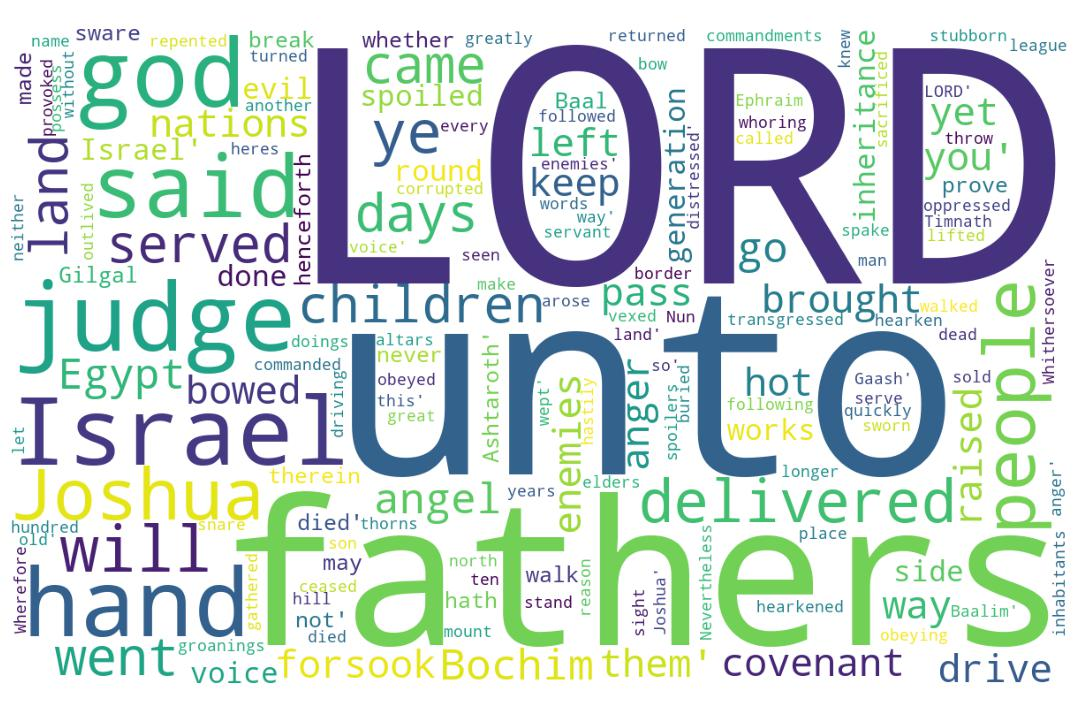
\includegraphics[width=\linewidth]{07OT-Judges/Judges2-WordCloud.jpg}
  \caption{Judges 2 Word Cloud}
  \label{fig:Judges 2 Word Cloud}
\end{figure}


\marginpar{\scriptsize \centering \fcolorbox{bone}{lime}{\textbf{COLLAPSE}}\\ (Judges 2:1-23) \begin{compactenum}[I.][8]
    \item   The \textbf{Covenant}  \index[scripture]{Judges!Jdg 02:01} (Jdg 2:1) 
    \item   The \textbf{Compromise}  \index[scripture]{Judges!Jdg 02:02} (Jdg 2:2) 
    \item   The \textbf{Crocodile Tears}  \index[scripture]{Judges!Jdg 02:04} (Jdg 2:4) 
    \item   The \textbf{Decline}  \index[scripture]{Judges!Jdg 02:10} (Jdg 2:10) 
    \item    \textbf{Corruption}  \index[scripture]{Judges!Jdg 02:11} (Jdg 2:11) 
    \item    \textbf{Collapse}  \index[scripture]{Judges!Jdg 02:12} (Jdg 2:12) 
    \item   The \textbf{Acrimony}  \index[scripture]{Judges!Jdg 02:14}\index[scripture]{Judges!Jdg 02:20} (Jdg 2:14, 20) 
    \item    \textbf{Champions}  \index[scripture]{Judges!Jdg 02:16} (Jdg 2:16) 
\end{compactenum}}

\marginpar{\scriptsize \centering \fcolorbox{bone}{yellow}{\textbf{HAVE IT YOUR WAY}}\\ (Judges 2:12-23) \begin{compactenum}[I.][8]
    \item   \textbf{Forsaking}  \index[scripture]{Judges!Jdg 02:12} (Jdg 2:12) 
    \item   \textbf{Following} other Gods  \index[scripture]{Judges!Jdg 02:12} (Jdg 2:12) 
    \item   \textbf{Falling Down}  \index[scripture]{Judges!Jdg 02:12} (Jdg 2:12) 
    \item   The \textbf{False}  Ones \index[scripture]{Judges!Jdg 02:13} (Jdg 2:13) 
    \item   \textbf{Enflaming} Anger \index[scripture]{Judges!Jdg 02:14} 
              \index[scripture]{Judges!Jdg 02:20} (Jdg 2:14, 20) 
    \item   The \textbf{Fruit}  Ones \index[scripture]{Judges!Jdg 02:16} (Jdg 2:16) 
    \item   \textbf{Five} Lords\index[scripture]{Judges!Jdg 03:03} (Jdg 3:3) 
\end{compactenum}}

\footnote{\textcolor[cmyk]{0.99998,1,0,0}{\hyperlink{TOC}{Return to end of Table of Contents.}}}\footnote{\href{https://audiobible.com/bible/judges_2.html}{\textcolor[cmyk]{0.99998,1,0,0}{Judges 2 Audio}}}\textcolor[cmyk]{0.99998,1,0,0}{And an angel of the LORD came up from Gilgal to Bochim, and said, I made you to go up out of Egypt, and have brought you \fcolorbox{bone}{bone}{unto} the land which I sware \fcolorbox{bone}{bone}{unto} your fathers; and I said, I will never break my \fcolorbox{bone}{lime}{covenant} with you.}
[2] \textcolor[cmyk]{0.99998,1,0,0}{And ye shall make no \fcolorbox{bone}{lime}{league} with the inhabitants of this land; ye shall throw down their altars: but ye have not obeyed my voice: why have ye done this?}
[3] \textcolor[cmyk]{0.99998,1,0,0}{Wherefore I also said, I will not drive them out from before you; but they shall be \emph{as} \emph{thorns} in your sides, and their gods shall be a snare \fcolorbox{bone}{bone}{unto} you.}
[4] \textcolor[cmyk]{0.99998,1,0,0}{And it came to pass, when the angel of the LORD spake these words \fcolorbox{bone}{bone}{unto} all the children of Israel, that the people lifted up their voice, and \fcolorbox{bone}{lime}{wept}.}
[5] \textcolor[cmyk]{0.99998,1,0,0}{And they called the name of that place Bochim: and they sacrificed there \fcolorbox{bone}{bone}{unto} the LORD.}\\
\\
\P \textcolor[cmyk]{0.99998,1,0,0}{And when Joshua had let the people go, the children of Israel went every man \fcolorbox{bone}{bone}{unto} his inheritance to possess the land.}
[7] \textcolor[cmyk]{0.99998,1,0,0}{And the people served the LORD all the days of Joshua, and all the days of the elders that outlived Joshua, who had seen all the great works of the LORD, that he did for Israel.}
[8] \textcolor[cmyk]{0.99998,1,0,0}{And Joshua the son of Nun, the servant of the LORD, died, \emph{being} an hundred and ten years old.}
[9] \textcolor[cmyk]{0.99998,1,0,0}{And they buried him in the border of his inheritance in Timnath-heres, in the mount of Ephraim, on the north side of the hill Gaash.}
[10] \textcolor[cmyk]{0.99998,1,0,0}{And also all that generation were gathered \fcolorbox{bone}{bone}{unto} their fathers: and there arose another generation after them, which \fcolorbox{bone}{lime}{knew not} the LORD, nor yet the works which he had done for Israel.}\\
\\
\P \textcolor[cmyk]{0.99998,1,0,0}{And the children of Israel did evil in the sight of the LORD, and \fcolorbox{bone}{lime}{served} \fcolorbox{bone}{lime}{Baalim}:}
[12] \textcolor[cmyk]{0.99998,1,0,0}{And they forsook the LORD God of their fathers, which brought them out of the land of Egypt, and followed other gods, of the gods of the people that \emph{were} round about them, and \fcolorbox{bone}{lime}{bowed themselves} \fcolorbox{bone}{bone}{unto} them, and provoked the LORD to anger.}
[13] \textcolor[cmyk]{0.99998,1,0,0}{And they forsook the LORD, and served Baal and Ashtaroth.}\\
\\
\P \textcolor[cmyk]{0.99998,1,0,0}{And the anger of the LORD was hot against Israel, and he \fcolorbox{bone}{lime}{delivered them} into the hands of spoilers that spoiled them, and he sold them into the hands of their enemies round about, so that they could not any longer stand before their enemies.}
[15] \textcolor[cmyk]{0.99998,1,0,0}{Whithersoever they went out, the hand of the LORD was against them for evil, as the LORD had said, and as the LORD had sworn \fcolorbox{bone}{bone}{unto} them: and they were greatly distressed.}\\
\\
\P \textcolor[cmyk]{0.99998,1,0,0}{Nevertheless the LORD raised up \fcolorbox{bone}{lime}{judges}, which delivered them out of the hand of those that spoiled them.}
[17] \textcolor[cmyk]{0.99998,1,0,0}{And yet they would not hearken \fcolorbox{bone}{bone}{unto} their judges, but they went a whoring after other gods, and bowed themselves \fcolorbox{bone}{bone}{unto} them: they turned quickly out of the way which their fathers walked in, obeying the commandments of the LORD; \emph{but} they did not so.}
[18] \textcolor[cmyk]{0.99998,1,0,0}{And when the LORD raised them up judges, then the LORD was with the judge, and delivered them out of the hand of their enemies all the days of the judge: for it repented the LORD because of their groanings by reason of them that oppressed them and vexed them.}
[19] \textcolor[cmyk]{0.99998,1,0,0}{And it came to pass, when the judge was dead, \emph{that} they returned, and corrupted \emph{themselves} more than their fathers, in following other gods to serve them, and to bow down \fcolorbox{bone}{bone}{unto} them; they ceased not from their own doings, nor from their stubborn way.}\\
\\
\P \textcolor[cmyk]{0.99998,1,0,0}{And the anger of the LORD was hot against Israel; and he said, Because that this people hath transgressed my covenant which I commanded their fathers, and have not hearkened \fcolorbox{bone}{bone}{unto} my voice;}
[21] \textcolor[cmyk]{0.99998,1,0,0}{I also will not henceforth drive out any from before them of the nations which Joshua left when he died:}
[22] \textcolor[cmyk]{0.99998,1,0,0}{That through them I may prove Israel, whether they will keep the way of the LORD to walk therein, as their fathers did keep \emph{it}, or not.}
[23] \textcolor[cmyk]{0.99998,1,0,0}{Therefore the LORD left those nations, without driving them out hastily; neither delivered he them into the hand of Joshua.}
\index[NWIV]{47!Judges!Jud 2:1}\index[AWIP]{And!Judges!Jud 2:1}\index[AWIP]{an!Judges!Jud 2:1}\index[AWIP]{angel!Judges!Jud 2:1}\index[AWIP]{of!Judges!Jud 2:1}\index[AWIP]{of!Judges!Jud 2:1 (2)}\index[AWIP]{the!Judges!Jud 2:1}\index[AWIP]{the!Judges!Jud 2:1 (2)}\index[AWIP]{LORD!Judges!Jud 2:1}\index[AWIP]{came!Judges!Jud 2:1}\index[AWIP]{up!Judges!Jud 2:1}\index[AWIP]{up!Judges!Jud 2:1 (2)}\index[AWIP]{from!Judges!Jud 2:1}\index[AWIP]{Gilgal!Judges!Jud 2:1}\index[AWIP]{to!Judges!Jud 2:1}\index[AWIP]{to!Judges!Jud 2:1 (2)}\index[AWIP]{Bochim!Judges!Jud 2:1}\index[AWIP]{and!Judges!Jud 2:1}\index[AWIP]{and!Judges!Jud 2:1 (2)}\index[AWIP]{and!Judges!Jud 2:1 (3)}\index[AWIP]{said!Judges!Jud 2:1}\index[AWIP]{said!Judges!Jud 2:1 (2)}\index[AWIP]{I!Judges!Jud 2:1}\index[AWIP]{I!Judges!Jud 2:1 (2)}\index[AWIP]{I!Judges!Jud 2:1 (3)}\index[AWIP]{I!Judges!Jud 2:1 (4)}\index[AWIP]{made!Judges!Jud 2:1}\index[AWIP]{you!Judges!Jud 2:1}\index[AWIP]{you!Judges!Jud 2:1 (2)}\index[AWIP]{you!Judges!Jud 2:1 (3)}\index[AWIP]{go!Judges!Jud 2:1}\index[AWIP]{out!Judges!Jud 2:1}\index[AWIP]{Egypt!Judges!Jud 2:1}\index[AWIP]{have!Judges!Jud 2:1}\index[AWIP]{brought!Judges!Jud 2:1}\index[AWIP]{unto!Judges!Jud 2:1}\index[AWIP]{unto!Judges!Jud 2:1 (2)}\index[AWIP]{land!Judges!Jud 2:1}\index[AWIP]{which!Judges!Jud 2:1}\index[AWIP]{sware!Judges!Jud 2:1}\index[AWIP]{your!Judges!Jud 2:1}\index[AWIP]{fathers!Judges!Jud 2:1}\index[AWIP]{will!Judges!Jud 2:1}\index[AWIP]{never!Judges!Jud 2:1}\index[AWIP]{break!Judges!Jud 2:1}\index[AWIP]{my!Judges!Jud 2:1}\index[AWIP]{covenant!Judges!Jud 2:1}\index[AWIP]{with!Judges!Jud 2:1}

\index[NWIV]{30!Judges!Jud 2:2}\index[AWIP]{And!Judges!Jud 2:2}\index[AWIP]{ye!Judges!Jud 2:2}\index[AWIP]{ye!Judges!Jud 2:2 (2)}\index[AWIP]{ye!Judges!Jud 2:2 (3)}\index[AWIP]{ye!Judges!Jud 2:2 (4)}\index[AWIP]{shall!Judges!Jud 2:2}\index[AWIP]{shall!Judges!Jud 2:2 (2)}\index[AWIP]{make!Judges!Jud 2:2}\index[AWIP]{no!Judges!Jud 2:2}\index[AWIP]{league!Judges!Jud 2:2}\index[AWIP]{with!Judges!Jud 2:2}\index[AWIP]{the!Judges!Jud 2:2}\index[AWIP]{inhabitants!Judges!Jud 2:2}\index[AWIP]{of!Judges!Jud 2:2}\index[AWIP]{this!Judges!Jud 2:2}\index[AWIP]{land!Judges!Jud 2:2}\index[AWIP]{throw!Judges!Jud 2:2}\index[AWIP]{down!Judges!Jud 2:2}\index[AWIP]{their!Judges!Jud 2:2}\index[AWIP]{altars!Judges!Jud 2:2}\index[AWIP]{but!Judges!Jud 2:2}\index[AWIP]{have!Judges!Jud 2:2}\index[AWIP]{have!Judges!Jud 2:2 (2)}\index[AWIP]{not!Judges!Jud 2:2}\index[AWIP]{obeyed!Judges!Jud 2:2}\index[AWIP]{my!Judges!Jud 2:2}\index[AWIP]{voice!Judges!Jud 2:2}\index[AWIP]{why!Judges!Jud 2:2}\index[AWIP]{done!Judges!Jud 2:2}\index[AWIP]{this?!Judges!Jud 2:2}

\index[NWIV]{31!Judges!Jud 2:3}\index[AWIP]{Wherefore!Judges!Jud 2:3}\index[AWIP]{I!Judges!Jud 2:3}\index[AWIP]{I!Judges!Jud 2:3 (2)}\index[AWIP]{also!Judges!Jud 2:3}\index[AWIP]{said!Judges!Jud 2:3}\index[AWIP]{will!Judges!Jud 2:3}\index[AWIP]{not!Judges!Jud 2:3}\index[AWIP]{drive!Judges!Jud 2:3}\index[AWIP]{them!Judges!Jud 2:3}\index[AWIP]{out!Judges!Jud 2:3}\index[AWIP]{from!Judges!Jud 2:3}\index[AWIP]{before!Judges!Jud 2:3}\index[AWIP]{you!Judges!Jud 2:3}\index[AWIP]{you!Judges!Jud 2:3 (2)}\index[AWIP]{but!Judges!Jud 2:3}\index[AWIP]{they!Judges!Jud 2:3}\index[AWIP]{shall!Judges!Jud 2:3}\index[AWIP]{shall!Judges!Jud 2:3 (2)}\index[AWIP]{be!Judges!Jud 2:3}\index[AWIP]{be!Judges!Jud 2:3 (2)}\index[AWIP]{\emph{as}!Judges!Jud 2:3}\index[AWIP]{\emph{thorns}!Judges!Jud 2:3}\index[AWIP]{in!Judges!Jud 2:3}\index[AWIP]{your!Judges!Jud 2:3}\index[AWIP]{sides!Judges!Jud 2:3}\index[AWIP]{and!Judges!Jud 2:3}\index[AWIP]{their!Judges!Jud 2:3}\index[AWIP]{gods!Judges!Jud 2:3}\index[AWIP]{a!Judges!Jud 2:3}\index[AWIP]{snare!Judges!Jud 2:3}\index[AWIP]{unto!Judges!Jud 2:3}\index[AWIP]{\emph{as}!Judges!Jud 2:3}\index[AWIP]{\emph{thorns}!Judges!Jud 2:3}

\index[NWIV]{29!Judges!Jud 2:4}\index[AWIP]{And!Judges!Jud 2:4}\index[AWIP]{it!Judges!Jud 2:4}\index[AWIP]{came!Judges!Jud 2:4}\index[AWIP]{to!Judges!Jud 2:4}\index[AWIP]{pass!Judges!Jud 2:4}\index[AWIP]{when!Judges!Jud 2:4}\index[AWIP]{the!Judges!Jud 2:4}\index[AWIP]{the!Judges!Jud 2:4 (2)}\index[AWIP]{the!Judges!Jud 2:4 (3)}\index[AWIP]{the!Judges!Jud 2:4 (4)}\index[AWIP]{angel!Judges!Jud 2:4}\index[AWIP]{of!Judges!Jud 2:4}\index[AWIP]{of!Judges!Jud 2:4 (2)}\index[AWIP]{LORD!Judges!Jud 2:4}\index[AWIP]{spake!Judges!Jud 2:4}\index[AWIP]{these!Judges!Jud 2:4}\index[AWIP]{words!Judges!Jud 2:4}\index[AWIP]{unto!Judges!Jud 2:4}\index[AWIP]{all!Judges!Jud 2:4}\index[AWIP]{children!Judges!Jud 2:4}\index[AWIP]{Israel!Judges!Jud 2:4}\index[AWIP]{that!Judges!Jud 2:4}\index[AWIP]{people!Judges!Jud 2:4}\index[AWIP]{lifted!Judges!Jud 2:4}\index[AWIP]{up!Judges!Jud 2:4}\index[AWIP]{their!Judges!Jud 2:4}\index[AWIP]{voice!Judges!Jud 2:4}\index[AWIP]{and!Judges!Jud 2:4}\index[AWIP]{wept!Judges!Jud 2:4}

\index[NWIV]{16!Judges!Jud 2:5}\index[AWIP]{And!Judges!Jud 2:5}\index[AWIP]{they!Judges!Jud 2:5}\index[AWIP]{they!Judges!Jud 2:5 (2)}\index[AWIP]{called!Judges!Jud 2:5}\index[AWIP]{the!Judges!Jud 2:5}\index[AWIP]{the!Judges!Jud 2:5 (2)}\index[AWIP]{name!Judges!Jud 2:5}\index[AWIP]{of!Judges!Jud 2:5}\index[AWIP]{that!Judges!Jud 2:5}\index[AWIP]{place!Judges!Jud 2:5}\index[AWIP]{Bochim!Judges!Jud 2:5}\index[AWIP]{and!Judges!Jud 2:5}\index[AWIP]{sacrificed!Judges!Jud 2:5}\index[AWIP]{there!Judges!Jud 2:5}\index[AWIP]{unto!Judges!Jud 2:5}\index[AWIP]{LORD!Judges!Jud 2:5}

\index[NWIV]{22!Judges!Jud 2:6}\index[AWIP]{And!Judges!Jud 2:6}\index[AWIP]{when!Judges!Jud 2:6}\index[AWIP]{Joshua!Judges!Jud 2:6}\index[AWIP]{had!Judges!Jud 2:6}\index[AWIP]{let!Judges!Jud 2:6}\index[AWIP]{the!Judges!Jud 2:6}\index[AWIP]{the!Judges!Jud 2:6 (2)}\index[AWIP]{the!Judges!Jud 2:6 (3)}\index[AWIP]{people!Judges!Jud 2:6}\index[AWIP]{go!Judges!Jud 2:6}\index[AWIP]{children!Judges!Jud 2:6}\index[AWIP]{of!Judges!Jud 2:6}\index[AWIP]{Israel!Judges!Jud 2:6}\index[AWIP]{went!Judges!Jud 2:6}\index[AWIP]{every!Judges!Jud 2:6}\index[AWIP]{man!Judges!Jud 2:6}\index[AWIP]{unto!Judges!Jud 2:6}\index[AWIP]{his!Judges!Jud 2:6}\index[AWIP]{inheritance!Judges!Jud 2:6}\index[AWIP]{to!Judges!Jud 2:6}\index[AWIP]{possess!Judges!Jud 2:6}\index[AWIP]{land!Judges!Jud 2:6}

\index[NWIV]{36!Judges!Jud 2:7}\index[AWIP]{And!Judges!Jud 2:7}\index[AWIP]{the!Judges!Jud 2:7}\index[AWIP]{the!Judges!Jud 2:7 (2)}\index[AWIP]{the!Judges!Jud 2:7 (3)}\index[AWIP]{the!Judges!Jud 2:7 (4)}\index[AWIP]{the!Judges!Jud 2:7 (5)}\index[AWIP]{the!Judges!Jud 2:7 (6)}\index[AWIP]{the!Judges!Jud 2:7 (7)}\index[AWIP]{people!Judges!Jud 2:7}\index[AWIP]{served!Judges!Jud 2:7}\index[AWIP]{LORD!Judges!Jud 2:7}\index[AWIP]{LORD!Judges!Jud 2:7 (2)}\index[AWIP]{all!Judges!Jud 2:7}\index[AWIP]{all!Judges!Jud 2:7 (2)}\index[AWIP]{all!Judges!Jud 2:7 (3)}\index[AWIP]{days!Judges!Jud 2:7}\index[AWIP]{days!Judges!Jud 2:7 (2)}\index[AWIP]{of!Judges!Jud 2:7}\index[AWIP]{of!Judges!Jud 2:7 (2)}\index[AWIP]{of!Judges!Jud 2:7 (3)}\index[AWIP]{Joshua!Judges!Jud 2:7}\index[AWIP]{Joshua!Judges!Jud 2:7 (2)}\index[AWIP]{and!Judges!Jud 2:7}\index[AWIP]{elders!Judges!Jud 2:7}\index[AWIP]{that!Judges!Jud 2:7}\index[AWIP]{that!Judges!Jud 2:7 (2)}\index[AWIP]{outlived!Judges!Jud 2:7}\index[AWIP]{who!Judges!Jud 2:7}\index[AWIP]{had!Judges!Jud 2:7}\index[AWIP]{seen!Judges!Jud 2:7}\index[AWIP]{great!Judges!Jud 2:7}\index[AWIP]{works!Judges!Jud 2:7}\index[AWIP]{he!Judges!Jud 2:7}\index[AWIP]{did!Judges!Jud 2:7}\index[AWIP]{for!Judges!Jud 2:7}\index[AWIP]{Israel!Judges!Jud 2:7}

\index[NWIV]{19!Judges!Jud 2:8}\index[AWIP]{And!Judges!Jud 2:8}\index[AWIP]{Joshua!Judges!Jud 2:8}\index[AWIP]{the!Judges!Jud 2:8}\index[AWIP]{the!Judges!Jud 2:8 (2)}\index[AWIP]{the!Judges!Jud 2:8 (3)}\index[AWIP]{son!Judges!Jud 2:8}\index[AWIP]{of!Judges!Jud 2:8}\index[AWIP]{of!Judges!Jud 2:8 (2)}\index[AWIP]{Nun!Judges!Jud 2:8}\index[AWIP]{servant!Judges!Jud 2:8}\index[AWIP]{LORD!Judges!Jud 2:8}\index[AWIP]{died!Judges!Jud 2:8}\index[AWIP]{\emph{being}!Judges!Jud 2:8}\index[AWIP]{an!Judges!Jud 2:8}\index[AWIP]{hundred!Judges!Jud 2:8}\index[AWIP]{and!Judges!Jud 2:8}\index[AWIP]{ten!Judges!Jud 2:8}\index[AWIP]{years!Judges!Jud 2:8}\index[AWIP]{old!Judges!Jud 2:8}\index[AWIP]{\emph{being}!Judges!Jud 2:8}

\index[NWIV]{25!Judges!Jud 2:9}\index[AWIP]{And!Judges!Jud 2:9}\index[AWIP]{they!Judges!Jud 2:9}\index[AWIP]{buried!Judges!Jud 2:9}\index[AWIP]{him!Judges!Jud 2:9}\index[AWIP]{in!Judges!Jud 2:9}\index[AWIP]{in!Judges!Jud 2:9 (2)}\index[AWIP]{in!Judges!Jud 2:9 (3)}\index[AWIP]{the!Judges!Jud 2:9}\index[AWIP]{the!Judges!Jud 2:9 (2)}\index[AWIP]{the!Judges!Jud 2:9 (3)}\index[AWIP]{the!Judges!Jud 2:9 (4)}\index[AWIP]{border!Judges!Jud 2:9}\index[AWIP]{of!Judges!Jud 2:9}\index[AWIP]{of!Judges!Jud 2:9 (2)}\index[AWIP]{of!Judges!Jud 2:9 (3)}\index[AWIP]{his!Judges!Jud 2:9}\index[AWIP]{inheritance!Judges!Jud 2:9}\index[AWIP]{Timnath-heres!Judges!Jud 2:9}\index[AWIP]{mount!Judges!Jud 2:9}\index[AWIP]{Ephraim!Judges!Jud 2:9}\index[AWIP]{on!Judges!Jud 2:9}\index[AWIP]{north!Judges!Jud 2:9}\index[AWIP]{side!Judges!Jud 2:9}\index[AWIP]{hill!Judges!Jud 2:9}\index[AWIP]{Gaash!Judges!Jud 2:9}

\index[NWIV]{32!Judges!Jud 2:10}\index[AWIP]{And!Judges!Jud 2:10}\index[AWIP]{also!Judges!Jud 2:10}\index[AWIP]{all!Judges!Jud 2:10}\index[AWIP]{that!Judges!Jud 2:10}\index[AWIP]{generation!Judges!Jud 2:10}\index[AWIP]{generation!Judges!Jud 2:10 (2)}\index[AWIP]{were!Judges!Jud 2:10}\index[AWIP]{gathered!Judges!Jud 2:10}\index[AWIP]{unto!Judges!Jud 2:10}\index[AWIP]{their!Judges!Jud 2:10}\index[AWIP]{fathers!Judges!Jud 2:10}\index[AWIP]{and!Judges!Jud 2:10}\index[AWIP]{there!Judges!Jud 2:10}\index[AWIP]{arose!Judges!Jud 2:10}\index[AWIP]{another!Judges!Jud 2:10}\index[AWIP]{after!Judges!Jud 2:10}\index[AWIP]{them!Judges!Jud 2:10}\index[AWIP]{which!Judges!Jud 2:10}\index[AWIP]{which!Judges!Jud 2:10 (2)}\index[AWIP]{knew!Judges!Jud 2:10}\index[AWIP]{not!Judges!Jud 2:10}\index[AWIP]{the!Judges!Jud 2:10}\index[AWIP]{the!Judges!Jud 2:10 (2)}\index[AWIP]{LORD!Judges!Jud 2:10}\index[AWIP]{nor!Judges!Jud 2:10}\index[AWIP]{yet!Judges!Jud 2:10}\index[AWIP]{works!Judges!Jud 2:10}\index[AWIP]{he!Judges!Jud 2:10}\index[AWIP]{had!Judges!Jud 2:10}\index[AWIP]{done!Judges!Jud 2:10}\index[AWIP]{for!Judges!Jud 2:10}\index[AWIP]{Israel!Judges!Jud 2:10}

\index[NWIV]{16!Judges!Jud 2:11}\index[AWIP]{And!Judges!Jud 2:11}\index[AWIP]{the!Judges!Jud 2:11}\index[AWIP]{the!Judges!Jud 2:11 (2)}\index[AWIP]{the!Judges!Jud 2:11 (3)}\index[AWIP]{children!Judges!Jud 2:11}\index[AWIP]{of!Judges!Jud 2:11}\index[AWIP]{of!Judges!Jud 2:11 (2)}\index[AWIP]{Israel!Judges!Jud 2:11}\index[AWIP]{did!Judges!Jud 2:11}\index[AWIP]{evil!Judges!Jud 2:11}\index[AWIP]{in!Judges!Jud 2:11}\index[AWIP]{sight!Judges!Jud 2:11}\index[AWIP]{LORD!Judges!Jud 2:11}\index[AWIP]{and!Judges!Jud 2:11}\index[AWIP]{served!Judges!Jud 2:11}\index[AWIP]{Baalim!Judges!Jud 2:11}

\index[NWIV]{44!Judges!Jud 2:12}\index[AWIP]{And!Judges!Jud 2:12}\index[AWIP]{they!Judges!Jud 2:12}\index[AWIP]{forsook!Judges!Jud 2:12}\index[AWIP]{the!Judges!Jud 2:12}\index[AWIP]{the!Judges!Jud 2:12 (2)}\index[AWIP]{the!Judges!Jud 2:12 (3)}\index[AWIP]{the!Judges!Jud 2:12 (4)}\index[AWIP]{the!Judges!Jud 2:12 (5)}\index[AWIP]{LORD!Judges!Jud 2:12}\index[AWIP]{LORD!Judges!Jud 2:12 (2)}\index[AWIP]{God!Judges!Jud 2:12}\index[AWIP]{of!Judges!Jud 2:12}\index[AWIP]{of!Judges!Jud 2:12 (2)}\index[AWIP]{of!Judges!Jud 2:12 (3)}\index[AWIP]{of!Judges!Jud 2:12 (4)}\index[AWIP]{of!Judges!Jud 2:12 (5)}\index[AWIP]{their!Judges!Jud 2:12}\index[AWIP]{fathers!Judges!Jud 2:12}\index[AWIP]{which!Judges!Jud 2:12}\index[AWIP]{brought!Judges!Jud 2:12}\index[AWIP]{them!Judges!Jud 2:12}\index[AWIP]{them!Judges!Jud 2:12 (2)}\index[AWIP]{them!Judges!Jud 2:12 (3)}\index[AWIP]{out!Judges!Jud 2:12}\index[AWIP]{land!Judges!Jud 2:12}\index[AWIP]{Egypt!Judges!Jud 2:12}\index[AWIP]{and!Judges!Jud 2:12}\index[AWIP]{and!Judges!Jud 2:12 (2)}\index[AWIP]{and!Judges!Jud 2:12 (3)}\index[AWIP]{followed!Judges!Jud 2:12}\index[AWIP]{other!Judges!Jud 2:12}\index[AWIP]{gods!Judges!Jud 2:12}\index[AWIP]{gods!Judges!Jud 2:12 (2)}\index[AWIP]{people!Judges!Jud 2:12}\index[AWIP]{that!Judges!Jud 2:12}\index[AWIP]{\emph{were}!Judges!Jud 2:12}\index[AWIP]{round!Judges!Jud 2:12}\index[AWIP]{about!Judges!Jud 2:12}\index[AWIP]{bowed!Judges!Jud 2:12}\index[AWIP]{themselves!Judges!Jud 2:12}\index[AWIP]{unto!Judges!Jud 2:12}\index[AWIP]{provoked!Judges!Jud 2:12}\index[AWIP]{to!Judges!Jud 2:12}\index[AWIP]{anger!Judges!Jud 2:12}\index[AWIP]{\emph{were}!Judges!Jud 2:12}

\index[NWIV]{10!Judges!Jud 2:13}\index[AWIP]{And!Judges!Jud 2:13}\index[AWIP]{they!Judges!Jud 2:13}\index[AWIP]{forsook!Judges!Jud 2:13}\index[AWIP]{the!Judges!Jud 2:13}\index[AWIP]{LORD!Judges!Jud 2:13}\index[AWIP]{and!Judges!Jud 2:13}\index[AWIP]{and!Judges!Jud 2:13 (2)}\index[AWIP]{served!Judges!Jud 2:13}\index[AWIP]{Baal!Judges!Jud 2:13}\index[AWIP]{Ashtaroth!Judges!Jud 2:13}

\index[NWIV]{45!Judges!Jud 2:14}\index[AWIP]{And!Judges!Jud 2:14}\index[AWIP]{the!Judges!Jud 2:14}\index[AWIP]{the!Judges!Jud 2:14 (2)}\index[AWIP]{the!Judges!Jud 2:14 (3)}\index[AWIP]{the!Judges!Jud 2:14 (4)}\index[AWIP]{anger!Judges!Jud 2:14}\index[AWIP]{of!Judges!Jud 2:14}\index[AWIP]{of!Judges!Jud 2:14 (2)}\index[AWIP]{of!Judges!Jud 2:14 (3)}\index[AWIP]{LORD!Judges!Jud 2:14}\index[AWIP]{was!Judges!Jud 2:14}\index[AWIP]{hot!Judges!Jud 2:14}\index[AWIP]{against!Judges!Jud 2:14}\index[AWIP]{Israel!Judges!Jud 2:14}\index[AWIP]{and!Judges!Jud 2:14}\index[AWIP]{and!Judges!Jud 2:14 (2)}\index[AWIP]{he!Judges!Jud 2:14}\index[AWIP]{he!Judges!Jud 2:14 (2)}\index[AWIP]{delivered!Judges!Jud 2:14}\index[AWIP]{them!Judges!Jud 2:14}\index[AWIP]{them!Judges!Jud 2:14 (2)}\index[AWIP]{them!Judges!Jud 2:14 (3)}\index[AWIP]{into!Judges!Jud 2:14}\index[AWIP]{into!Judges!Jud 2:14 (2)}\index[AWIP]{hands!Judges!Jud 2:14}\index[AWIP]{hands!Judges!Jud 2:14 (2)}\index[AWIP]{spoilers!Judges!Jud 2:14}\index[AWIP]{that!Judges!Jud 2:14}\index[AWIP]{that!Judges!Jud 2:14 (2)}\index[AWIP]{spoiled!Judges!Jud 2:14}\index[AWIP]{sold!Judges!Jud 2:14}\index[AWIP]{their!Judges!Jud 2:14}\index[AWIP]{their!Judges!Jud 2:14 (2)}\index[AWIP]{enemies!Judges!Jud 2:14}\index[AWIP]{enemies!Judges!Jud 2:14 (2)}\index[AWIP]{round!Judges!Jud 2:14}\index[AWIP]{about!Judges!Jud 2:14}\index[AWIP]{so!Judges!Jud 2:14}\index[AWIP]{they!Judges!Jud 2:14}\index[AWIP]{could!Judges!Jud 2:14}\index[AWIP]{not!Judges!Jud 2:14}\index[AWIP]{any!Judges!Jud 2:14}\index[AWIP]{longer!Judges!Jud 2:14}\index[AWIP]{stand!Judges!Jud 2:14}\index[AWIP]{before!Judges!Jud 2:14}

\index[NWIV]{32!Judges!Jud 2:15}\index[AWIP]{Whithersoever!Judges!Jud 2:15}\index[AWIP]{they!Judges!Jud 2:15}\index[AWIP]{they!Judges!Jud 2:15 (2)}\index[AWIP]{went!Judges!Jud 2:15}\index[AWIP]{out!Judges!Jud 2:15}\index[AWIP]{the!Judges!Jud 2:15}\index[AWIP]{the!Judges!Jud 2:15 (2)}\index[AWIP]{the!Judges!Jud 2:15 (3)}\index[AWIP]{the!Judges!Jud 2:15 (4)}\index[AWIP]{hand!Judges!Jud 2:15}\index[AWIP]{of!Judges!Jud 2:15}\index[AWIP]{LORD!Judges!Jud 2:15}\index[AWIP]{LORD!Judges!Jud 2:15 (2)}\index[AWIP]{LORD!Judges!Jud 2:15 (3)}\index[AWIP]{was!Judges!Jud 2:15}\index[AWIP]{against!Judges!Jud 2:15}\index[AWIP]{them!Judges!Jud 2:15}\index[AWIP]{them!Judges!Jud 2:15 (2)}\index[AWIP]{for!Judges!Jud 2:15}\index[AWIP]{evil!Judges!Jud 2:15}\index[AWIP]{as!Judges!Jud 2:15}\index[AWIP]{as!Judges!Jud 2:15 (2)}\index[AWIP]{had!Judges!Jud 2:15}\index[AWIP]{had!Judges!Jud 2:15 (2)}\index[AWIP]{said!Judges!Jud 2:15}\index[AWIP]{and!Judges!Jud 2:15}\index[AWIP]{and!Judges!Jud 2:15 (2)}\index[AWIP]{sworn!Judges!Jud 2:15}\index[AWIP]{unto!Judges!Jud 2:15}\index[AWIP]{were!Judges!Jud 2:15}\index[AWIP]{greatly!Judges!Jud 2:15}\index[AWIP]{distressed!Judges!Jud 2:15}

\index[NWIV]{18!Judges!Jud 2:16}\index[AWIP]{Nevertheless!Judges!Jud 2:16}\index[AWIP]{the!Judges!Jud 2:16}\index[AWIP]{the!Judges!Jud 2:16 (2)}\index[AWIP]{LORD!Judges!Jud 2:16}\index[AWIP]{raised!Judges!Jud 2:16}\index[AWIP]{up!Judges!Jud 2:16}\index[AWIP]{judges!Judges!Jud 2:16}\index[AWIP]{which!Judges!Jud 2:16}\index[AWIP]{delivered!Judges!Jud 2:16}\index[AWIP]{them!Judges!Jud 2:16}\index[AWIP]{them!Judges!Jud 2:16 (2)}\index[AWIP]{out!Judges!Jud 2:16}\index[AWIP]{of!Judges!Jud 2:16}\index[AWIP]{of!Judges!Jud 2:16 (2)}\index[AWIP]{hand!Judges!Jud 2:16}\index[AWIP]{those!Judges!Jud 2:16}\index[AWIP]{that!Judges!Jud 2:16}\index[AWIP]{spoiled!Judges!Jud 2:16}

\index[NWIV]{45!Judges!Jud 2:17}\index[AWIP]{And!Judges!Jud 2:17}\index[AWIP]{yet!Judges!Jud 2:17}\index[AWIP]{they!Judges!Jud 2:17}\index[AWIP]{they!Judges!Jud 2:17 (2)}\index[AWIP]{they!Judges!Jud 2:17 (3)}\index[AWIP]{they!Judges!Jud 2:17 (4)}\index[AWIP]{would!Judges!Jud 2:17}\index[AWIP]{not!Judges!Jud 2:17}\index[AWIP]{not!Judges!Jud 2:17 (2)}\index[AWIP]{hearken!Judges!Jud 2:17}\index[AWIP]{unto!Judges!Jud 2:17}\index[AWIP]{unto!Judges!Jud 2:17 (2)}\index[AWIP]{their!Judges!Jud 2:17}\index[AWIP]{their!Judges!Jud 2:17 (2)}\index[AWIP]{judges!Judges!Jud 2:17}\index[AWIP]{but!Judges!Jud 2:17}\index[AWIP]{went!Judges!Jud 2:17}\index[AWIP]{a!Judges!Jud 2:17}\index[AWIP]{whoring!Judges!Jud 2:17}\index[AWIP]{after!Judges!Jud 2:17}\index[AWIP]{other!Judges!Jud 2:17}\index[AWIP]{gods!Judges!Jud 2:17}\index[AWIP]{and!Judges!Jud 2:17}\index[AWIP]{bowed!Judges!Jud 2:17}\index[AWIP]{themselves!Judges!Jud 2:17}\index[AWIP]{them!Judges!Jud 2:17}\index[AWIP]{turned!Judges!Jud 2:17}\index[AWIP]{quickly!Judges!Jud 2:17}\index[AWIP]{out!Judges!Jud 2:17}\index[AWIP]{of!Judges!Jud 2:17}\index[AWIP]{of!Judges!Jud 2:17 (2)}\index[AWIP]{the!Judges!Jud 2:17}\index[AWIP]{the!Judges!Jud 2:17 (2)}\index[AWIP]{the!Judges!Jud 2:17 (3)}\index[AWIP]{way!Judges!Jud 2:17}\index[AWIP]{which!Judges!Jud 2:17}\index[AWIP]{fathers!Judges!Jud 2:17}\index[AWIP]{walked!Judges!Jud 2:17}\index[AWIP]{in!Judges!Jud 2:17}\index[AWIP]{obeying!Judges!Jud 2:17}\index[AWIP]{commandments!Judges!Jud 2:17}\index[AWIP]{LORD!Judges!Jud 2:17}\index[AWIP]{\emph{but}!Judges!Jud 2:17}\index[AWIP]{did!Judges!Jud 2:17}\index[AWIP]{so!Judges!Jud 2:17}\index[AWIP]{\emph{but}!Judges!Jud 2:17}

\index[NWIV]{50!Judges!Jud 2:18}\index[AWIP]{And!Judges!Jud 2:18}\index[AWIP]{when!Judges!Jud 2:18}\index[AWIP]{the!Judges!Jud 2:18}\index[AWIP]{the!Judges!Jud 2:18 (2)}\index[AWIP]{the!Judges!Jud 2:18 (3)}\index[AWIP]{the!Judges!Jud 2:18 (4)}\index[AWIP]{the!Judges!Jud 2:18 (5)}\index[AWIP]{the!Judges!Jud 2:18 (6)}\index[AWIP]{the!Judges!Jud 2:18 (7)}\index[AWIP]{LORD!Judges!Jud 2:18}\index[AWIP]{LORD!Judges!Jud 2:18 (2)}\index[AWIP]{LORD!Judges!Jud 2:18 (3)}\index[AWIP]{raised!Judges!Jud 2:18}\index[AWIP]{them!Judges!Jud 2:18}\index[AWIP]{them!Judges!Jud 2:18 (2)}\index[AWIP]{them!Judges!Jud 2:18 (3)}\index[AWIP]{them!Judges!Jud 2:18 (4)}\index[AWIP]{them!Judges!Jud 2:18 (5)}\index[AWIP]{up!Judges!Jud 2:18}\index[AWIP]{judges!Judges!Jud 2:18}\index[AWIP]{then!Judges!Jud 2:18}\index[AWIP]{was!Judges!Jud 2:18}\index[AWIP]{with!Judges!Jud 2:18}\index[AWIP]{judge!Judges!Jud 2:18}\index[AWIP]{judge!Judges!Jud 2:18 (2)}\index[AWIP]{and!Judges!Jud 2:18}\index[AWIP]{and!Judges!Jud 2:18 (2)}\index[AWIP]{delivered!Judges!Jud 2:18}\index[AWIP]{out!Judges!Jud 2:18}\index[AWIP]{of!Judges!Jud 2:18}\index[AWIP]{of!Judges!Jud 2:18 (2)}\index[AWIP]{of!Judges!Jud 2:18 (3)}\index[AWIP]{of!Judges!Jud 2:18 (4)}\index[AWIP]{of!Judges!Jud 2:18 (5)}\index[AWIP]{hand!Judges!Jud 2:18}\index[AWIP]{their!Judges!Jud 2:18}\index[AWIP]{their!Judges!Jud 2:18 (2)}\index[AWIP]{enemies!Judges!Jud 2:18}\index[AWIP]{all!Judges!Jud 2:18}\index[AWIP]{days!Judges!Jud 2:18}\index[AWIP]{for!Judges!Jud 2:18}\index[AWIP]{it!Judges!Jud 2:18}\index[AWIP]{repented!Judges!Jud 2:18}\index[AWIP]{because!Judges!Jud 2:18}\index[AWIP]{groanings!Judges!Jud 2:18}\index[AWIP]{by!Judges!Jud 2:18}\index[AWIP]{reason!Judges!Jud 2:18}\index[AWIP]{that!Judges!Jud 2:18}\index[AWIP]{oppressed!Judges!Jud 2:18}\index[AWIP]{vexed!Judges!Jud 2:18}

\index[NWIV]{45!Judges!Jud 2:19}\index[AWIP]{And!Judges!Jud 2:19}\index[AWIP]{it!Judges!Jud 2:19}\index[AWIP]{came!Judges!Jud 2:19}\index[AWIP]{to!Judges!Jud 2:19}\index[AWIP]{to!Judges!Jud 2:19 (2)}\index[AWIP]{to!Judges!Jud 2:19 (3)}\index[AWIP]{pass!Judges!Jud 2:19}\index[AWIP]{when!Judges!Jud 2:19}\index[AWIP]{the!Judges!Jud 2:19}\index[AWIP]{judge!Judges!Jud 2:19}\index[AWIP]{was!Judges!Jud 2:19}\index[AWIP]{dead!Judges!Jud 2:19}\index[AWIP]{\emph{that}!Judges!Jud 2:19}\index[AWIP]{they!Judges!Jud 2:19}\index[AWIP]{they!Judges!Jud 2:19 (2)}\index[AWIP]{returned!Judges!Jud 2:19}\index[AWIP]{and!Judges!Jud 2:19}\index[AWIP]{and!Judges!Jud 2:19 (2)}\index[AWIP]{corrupted!Judges!Jud 2:19}\index[AWIP]{\emph{themselves}!Judges!Jud 2:19}\index[AWIP]{more!Judges!Jud 2:19}\index[AWIP]{than!Judges!Jud 2:19}\index[AWIP]{their!Judges!Jud 2:19}\index[AWIP]{their!Judges!Jud 2:19 (2)}\index[AWIP]{their!Judges!Jud 2:19 (3)}\index[AWIP]{fathers!Judges!Jud 2:19}\index[AWIP]{in!Judges!Jud 2:19}\index[AWIP]{following!Judges!Jud 2:19}\index[AWIP]{other!Judges!Jud 2:19}\index[AWIP]{gods!Judges!Jud 2:19}\index[AWIP]{serve!Judges!Jud 2:19}\index[AWIP]{them!Judges!Jud 2:19}\index[AWIP]{them!Judges!Jud 2:19 (2)}\index[AWIP]{bow!Judges!Jud 2:19}\index[AWIP]{down!Judges!Jud 2:19}\index[AWIP]{unto!Judges!Jud 2:19}\index[AWIP]{ceased!Judges!Jud 2:19}\index[AWIP]{not!Judges!Jud 2:19}\index[AWIP]{from!Judges!Jud 2:19}\index[AWIP]{from!Judges!Jud 2:19 (2)}\index[AWIP]{own!Judges!Jud 2:19}\index[AWIP]{doings!Judges!Jud 2:19}\index[AWIP]{nor!Judges!Jud 2:19}\index[AWIP]{stubborn!Judges!Jud 2:19}\index[AWIP]{way!Judges!Jud 2:19}\index[AWIP]{\emph{that}!Judges!Jud 2:19}\index[AWIP]{\emph{themselves}!Judges!Jud 2:19}

\index[NWIV]{33!Judges!Jud 2:20}\index[AWIP]{And!Judges!Jud 2:20}\index[AWIP]{the!Judges!Jud 2:20}\index[AWIP]{the!Judges!Jud 2:20 (2)}\index[AWIP]{anger!Judges!Jud 2:20}\index[AWIP]{of!Judges!Jud 2:20}\index[AWIP]{LORD!Judges!Jud 2:20}\index[AWIP]{was!Judges!Jud 2:20}\index[AWIP]{hot!Judges!Jud 2:20}\index[AWIP]{against!Judges!Jud 2:20}\index[AWIP]{Israel!Judges!Jud 2:20}\index[AWIP]{and!Judges!Jud 2:20}\index[AWIP]{and!Judges!Jud 2:20 (2)}\index[AWIP]{he!Judges!Jud 2:20}\index[AWIP]{said!Judges!Jud 2:20}\index[AWIP]{Because!Judges!Jud 2:20}\index[AWIP]{that!Judges!Jud 2:20}\index[AWIP]{this!Judges!Jud 2:20}\index[AWIP]{people!Judges!Jud 2:20}\index[AWIP]{hath!Judges!Jud 2:20}\index[AWIP]{transgressed!Judges!Jud 2:20}\index[AWIP]{my!Judges!Jud 2:20}\index[AWIP]{my!Judges!Jud 2:20 (2)}\index[AWIP]{covenant!Judges!Jud 2:20}\index[AWIP]{which!Judges!Jud 2:20}\index[AWIP]{I!Judges!Jud 2:20}\index[AWIP]{commanded!Judges!Jud 2:20}\index[AWIP]{their!Judges!Jud 2:20}\index[AWIP]{fathers!Judges!Jud 2:20}\index[AWIP]{have!Judges!Jud 2:20}\index[AWIP]{not!Judges!Jud 2:20}\index[AWIP]{hearkened!Judges!Jud 2:20}\index[AWIP]{unto!Judges!Jud 2:20}\index[AWIP]{voice!Judges!Jud 2:20}

\index[NWIV]{20!Judges!Jud 2:21}\index[AWIP]{I!Judges!Jud 2:21}\index[AWIP]{also!Judges!Jud 2:21}\index[AWIP]{will!Judges!Jud 2:21}\index[AWIP]{not!Judges!Jud 2:21}\index[AWIP]{henceforth!Judges!Jud 2:21}\index[AWIP]{drive!Judges!Jud 2:21}\index[AWIP]{out!Judges!Jud 2:21}\index[AWIP]{any!Judges!Jud 2:21}\index[AWIP]{from!Judges!Jud 2:21}\index[AWIP]{before!Judges!Jud 2:21}\index[AWIP]{them!Judges!Jud 2:21}\index[AWIP]{of!Judges!Jud 2:21}\index[AWIP]{the!Judges!Jud 2:21}\index[AWIP]{nations!Judges!Jud 2:21}\index[AWIP]{which!Judges!Jud 2:21}\index[AWIP]{Joshua!Judges!Jud 2:21}\index[AWIP]{left!Judges!Jud 2:21}\index[AWIP]{when!Judges!Jud 2:21}\index[AWIP]{he!Judges!Jud 2:21}\index[AWIP]{died!Judges!Jud 2:21}

\index[NWIV]{27!Judges!Jud 2:22}\index[AWIP]{That!Judges!Jud 2:22}\index[AWIP]{through!Judges!Jud 2:22}\index[AWIP]{them!Judges!Jud 2:22}\index[AWIP]{I!Judges!Jud 2:22}\index[AWIP]{may!Judges!Jud 2:22}\index[AWIP]{prove!Judges!Jud 2:22}\index[AWIP]{Israel!Judges!Jud 2:22}\index[AWIP]{whether!Judges!Jud 2:22}\index[AWIP]{they!Judges!Jud 2:22}\index[AWIP]{will!Judges!Jud 2:22}\index[AWIP]{keep!Judges!Jud 2:22}\index[AWIP]{keep!Judges!Jud 2:22 (2)}\index[AWIP]{the!Judges!Jud 2:22}\index[AWIP]{the!Judges!Jud 2:22 (2)}\index[AWIP]{way!Judges!Jud 2:22}\index[AWIP]{of!Judges!Jud 2:22}\index[AWIP]{LORD!Judges!Jud 2:22}\index[AWIP]{to!Judges!Jud 2:22}\index[AWIP]{walk!Judges!Jud 2:22}\index[AWIP]{therein!Judges!Jud 2:22}\index[AWIP]{as!Judges!Jud 2:22}\index[AWIP]{their!Judges!Jud 2:22}\index[AWIP]{fathers!Judges!Jud 2:22}\index[AWIP]{did!Judges!Jud 2:22}\index[AWIP]{\emph{it}!Judges!Jud 2:22}\index[AWIP]{or!Judges!Jud 2:22}\index[AWIP]{not!Judges!Jud 2:22}\index[AWIP]{\emph{it}!Judges!Jud 2:22}

\index[NWIV]{20!Judges!Jud 2:23}\index[AWIP]{Therefore!Judges!Jud 2:23}\index[AWIP]{the!Judges!Jud 2:23}\index[AWIP]{the!Judges!Jud 2:23 (2)}\index[AWIP]{LORD!Judges!Jud 2:23}\index[AWIP]{left!Judges!Jud 2:23}\index[AWIP]{those!Judges!Jud 2:23}\index[AWIP]{nations!Judges!Jud 2:23}\index[AWIP]{without!Judges!Jud 2:23}\index[AWIP]{driving!Judges!Jud 2:23}\index[AWIP]{them!Judges!Jud 2:23}\index[AWIP]{them!Judges!Jud 2:23 (2)}\index[AWIP]{out!Judges!Jud 2:23}\index[AWIP]{hastily!Judges!Jud 2:23}\index[AWIP]{neither!Judges!Jud 2:23}\index[AWIP]{delivered!Judges!Jud 2:23}\index[AWIP]{he!Judges!Jud 2:23}\index[AWIP]{into!Judges!Jud 2:23}\index[AWIP]{hand!Judges!Jud 2:23}\index[AWIP]{of!Judges!Jud 2:23}\index[AWIP]{Joshua!Judges!Jud 2:23}


\section{Judges 2 Outlines}

\subsection{My Outlines}

\subsubsection{Collapse}
\index[speaker]{Keith Anthony!Judges 02 (Collapse) }
\index[series]{Judges (Keith Anthony)!Judges 02 (Collapse) }
\index[date]{2018/03/15!Judges 02 (Collapse) (Keith Anthony)}
\begin{compactenum}[I.][8]
    \item   The \textbf{Covenant}  \index[scripture]{Judges!Jdg 02:01} (Jdg 2:1) 
    \item   The \textbf{Compromise}  \index[scripture]{Judges!Jdg 02:02} (Jdg 2:2) 
    \item   The \textbf{Crocodile Tears}  \index[scripture]{Judges!Jdg 02:04} (Jdg 2:4) 
    \item   The \textbf{Decline}  \index[scripture]{Judges!Jdg 02:10} (Jdg 2:10) 
    \item    \textbf{Corruption}  \index[scripture]{Judges!Jdg 02:11} (Jdg 2:11) 
    \item    \textbf{Collapse}  \index[scripture]{Judges!Jdg 02:12} (Jdg 2:12) 
    \item   The \textbf{Acrimony}  \index[scripture]{Judges!Jdg 02:14}\index[scripture]{Judges!Jdg 02:20} (Jdg 2:14, 20) 
    \item    \textbf{Champions}  \index[scripture]{Judges!Jdg 02:16} (Jdg 2:16) 
\end{compactenum}


\subsubsection{Have it Your Way}
\index[speaker]{Keith Anthony!Judges 02 (Have it Your Way) }
\index[series]{Judges (Keith Anthony)!Judges 02 (Have it Your Way) }
\index[date]{2020/03/14!Judges 02 (Have it Your Way) (Keith Anthony)} \begin{compactenum}[I.][8]
    \item   \textbf{Forsaking}  \index[scripture]{Judges!Jdg 02:12} (Jdg 2:12) 
    \item   \textbf{Following} other Gods  \index[scripture]{Judges!Jdg 02:12} (Jdg 2:12) 
    \item   \textbf{Falling Down}  \index[scripture]{Judges!Jdg 02:12} (Jdg 2:12) 
    \item   The \textbf{False}  Ones \index[scripture]{Judges!Jdg 02:13} (Jdg 2:13) 
    \item   \textbf{Enflaming} Anger \index[scripture]{Judges!Jdg 02:14} 
              \index[scripture]{Judges!Jdg 02:20} (Jdg 2:14, 20) 
    \item   The \textbf{Fruit}  Ones \index[scripture]{Judges!Jdg 02:16} (Jdg 2:16) 
    \item   \textbf{Five} Lords\index[scripture]{Judges!Jdg 03:03} (Jdg 3:3) 
\end{compactenum}
\subsection{Outlines from Others}
\section{Judges 2 Comments}

\subsection{Numeric Nuggets}
\textbf{13: } Verse 11 has 13 unique words. he word ``unto'' is used 13 times in the chapter. 
\subsection{Judges 2 Repeated Phrases}


%%%%%%%%%%
%%%%%%%%%%
\normalsize
 
\begin{center}
\begin{longtable}{|p{3.0in}|p{0.5in}|}
\caption[Judges 2 Repeated Phrases]{Judges 2 Repeated Phrases}\label{table:Repeated Phrases Judges 2} \\
\hline \multicolumn{1}{|c|}{\textbf{Phrase}} & \multicolumn{1}{c|}{\textbf{Frequency}} \\ \hline 
\endfirsthead
 
\multicolumn{2}{c}
{{\bfseries \tablename\ \thetable{} -- continued from previous page}} \\  
\hline \multicolumn{1}{|c|}{\textbf{Phrase}} & \multicolumn{1}{c|}{\textbf{Frequency}} \\ \hline 
\endhead
 
\hline \multicolumn{2}{c}{{ }} \\ \hline
\endfoot 
the LORD & 23\\ \hline 
of the & 20\\ \hline 
of the LORD & 10\\ \hline 
their fathers & 6\\ \hline 
them and & 6\\ \hline 
out of & 5\\ \hline 
them out & 5\\ \hline 
all the & 5\\ \hline 
the people & 4\\ \hline 
And they & 4\\ \hline 
And the & 4\\ \hline 
of their & 4\\ \hline 
out of the & 4\\ \hline 
unto them & 4\\ \hline 
the LORD was & 4\\ \hline 
LORD was & 4\\ \hline 
the hand & 4\\ \hline 
the hand of & 4\\ \hline 
hand of & 4\\ \hline 
said I & 3\\ \hline 
the land & 3\\ \hline 
fathers and & 3\\ \hline 
when the & 3\\ \hline 
the children & 3\\ \hline 
the children of & 3\\ \hline 
the children of Israel & 3\\ \hline 
children of & 3\\ \hline 
children of Israel & 3\\ \hline 
of Israel & 3\\ \hline 
all the days & 3\\ \hline 
all the days of & 3\\ \hline 
the days & 3\\ \hline 
the days of & 3\\ \hline 
days of & 3\\ \hline 
in the & 3\\ \hline 
them out of & 3\\ \hline 
them out of the & 3\\ \hline 
other gods & 3\\ \hline 
of the LORD was & 3\\ \hline 
and he & 3\\ \hline 
delivered them & 3\\ \hline 
them into & 3\\ \hline 
them into the & 3\\ \hline 
into the & 3\\ \hline 
their enemies & 3\\ \hline 
the judge & 3\\ \hline 
\end{longtable}
\end{center}



%%%%%%%%%%
%%%%%%%%%%



\section{Judges 2 Statistics}

%%%%%%%%%%%%%%%%%%%%%%%%%%%
%%%%% Word Statistics
%%%%%%%%%%%%%%%%%%%%%%%%%%


\normalsize



\subsection{Chapter Word Statistics}


%%%%%%%%%%
%%%%%%%%%%
 
\begin{center}
\begin{longtable}{l|c|c|c|c}
\caption[Stats for Judges 2]{Stats for Judges 2} \label{table:Stats for Judges 2} \\ 
\hline \multicolumn{1}{|c|}{\textbf{Verse(s)}} & \multicolumn{1}{|c|}{\textbf{Count}} & \multicolumn{1}{|c|}{\textbf{Unique}} & \multicolumn{1}{|c|}{\textbf{Italics}} & \multicolumn{1}{|c|}{\textbf{Uniq Italic}}  \\ \hline 
\endfirsthead
 
\multicolumn{5}{c}
{{\bfseries \tablename\ \thetable{} -- continued from previous page}} \\  
\hline \multicolumn{1}{|c|}{\textbf{Verse(s)}} & \multicolumn{1}{|c|}{\textbf{Count}} & \multicolumn{1}{|c|}{\textbf{Unique}} & \multicolumn{1}{|c|}{\textbf{Italics}} & \multicolumn{1}{|c|}{\textbf{Uniq Italic}}  \\ \hline 
\endhead
 
\hline \multicolumn{5}{|r|}{{Continued if needed}} \\ \hline
\endfoot 
1 & 47 & 34 & 0 & 0\\ \hline
2 & 30 & 24 & 0 & 0\\ \hline
3 & 31 & 27 & 2 & 2\\ \hline
4 & 29 & 25 & 0 & 0\\ \hline
5 & 16 & 14 & 0 & 0\\ \hline
6 & 22 & 20 & 0 & 0\\ \hline
7 & 36 & 22 & 0 & 0\\ \hline
8 & 19 & 16 & 1 & 1\\ \hline
9 & 25 & 18 & 0 & 0\\ \hline
10 & 32 & 29 & 0 & 0\\ \hline
11 & 16 & 13 & 0 & 0\\ \hline
12 & 44 & 30 & 1 & 1\\ \hline
13 & 10 & 9 & 0 & 0\\ \hline
14 & 45 & 31 & 0 & 0\\ \hline
15 & 32 & 22 & 0 & 0\\ \hline
16 & 18 & 15 & 0 & 0\\ \hline
17 & 45 & 36 & 1 & 1\\ \hline
18 & 50 & 31 & 0 & 0\\ \hline
19 & 45 & 37 & 2 & 2\\ \hline
20 & 33 & 30 & 0 & 0\\ \hline
21 & 20 & 20 & 0 & 0\\ \hline
22 & 27 & 25 & 1 & 1\\ \hline
23 & 20 & 18 & 0 & 0\\ \hline
\hline \hline
Total & 692 & 229 & 8 & 8



\end{longtable}
\end{center}

%%%%%%%%%%
%%%%%%%%%%
 
\subsection{Words by Frequency}

\begin{center}
\begin{longtable}{l|r}
\caption[Word Frequencies in Judges 2]{Word Frequencies in Judges 2} \label{table:WordsIn-Judges-2} \\ 
\hline \multicolumn{1}{|c|}{\textbf{Word}} & \multicolumn{1}{c|}{\textbf{Frequency}} \\ \hline 
\endfirsthead
 
\multicolumn{2}{c}
{{\bfseries \tablename\ \thetable{} -- continued from previous page}} \\ 
\hline \multicolumn{1}{|c|}{\textbf{Word}} & \multicolumn{1}{c|}{\textbf{Frequency}} \\ \hline 
\endhead
 
\hline \multicolumn{2}{|r|}{{Continued if needed}} \\ \hline
\endfoot
 
\hline \hline
\endlastfoot
the & 65 \\ \hline
of & 39 \\ \hline
and & 26 \\ \hline
them & 24 \\ \hline
LORD & 23 \\ \hline
And & 17 \\ \hline
their & 16 \\ \hline
they & 16 \\ \hline
unto & 13 \\ \hline
that & 11 \\ \hline
not & 10 \\ \hline
to & 9 \\ \hline
I & 9 \\ \hline
out & 9 \\ \hline
which & 8 \\ \hline
Israel & 8 \\ \hline
fathers & 7 \\ \hline
in & 7 \\ \hline
he & 7 \\ \hline
all & 6 \\ \hline
Joshua & 6 \\ \hline
up & 5 \\ \hline
from & 5 \\ \hline
said & 5 \\ \hline
you & 5 \\ \hline
gods & 5 \\ \hline
when & 5 \\ \hline
people & 5 \\ \hline
had & 5 \\ \hline
was & 5 \\ \hline
have & 4 \\ \hline
land & 4 \\ \hline
will & 4 \\ \hline
my & 4 \\ \hline
ye & 4 \\ \hline
shall & 4 \\ \hline
did & 4 \\ \hline
for & 4 \\ \hline
delivered & 4 \\ \hline
hand & 4 \\ \hline
came & 3 \\ \hline
with & 3 \\ \hline
this & 3 \\ \hline
but & 3 \\ \hline
voice & 3 \\ \hline
also & 3 \\ \hline
before & 3 \\ \hline
it & 3 \\ \hline
children & 3 \\ \hline
went & 3 \\ \hline
served & 3 \\ \hline
days & 3 \\ \hline
other & 3 \\ \hline
anger & 3 \\ \hline
against & 3 \\ \hline
into & 3 \\ \hline
enemies & 3 \\ \hline
as & 3 \\ \hline
judges & 3 \\ \hline
way & 3 \\ \hline
judge & 3 \\ \hline
an & 2 \\ \hline
angel & 2 \\ \hline
Bochim & 2 \\ \hline
go & 2 \\ \hline
Egypt & 2 \\ \hline
brought & 2 \\ \hline
your & 2 \\ \hline
covenant & 2 \\ \hline
down & 2 \\ \hline
done & 2 \\ \hline
drive & 2 \\ \hline
be & 2 \\ \hline
a & 2 \\ \hline
pass & 2 \\ \hline
there & 2 \\ \hline
his & 2 \\ \hline
inheritance & 2 \\ \hline
works & 2 \\ \hline
died & 2 \\ \hline
generation & 2 \\ \hline
were & 2 \\ \hline
after & 2 \\ \hline
nor & 2 \\ \hline
yet & 2 \\ \hline
evil & 2 \\ \hline
forsook & 2 \\ \hline
round & 2 \\ \hline
about & 2 \\ \hline
bowed & 2 \\ \hline
themselves & 2 \\ \hline
hot & 2 \\ \hline
hands & 2 \\ \hline
spoiled & 2 \\ \hline
so & 2 \\ \hline
any & 2 \\ \hline
raised & 2 \\ \hline
those & 2 \\ \hline
nations & 2 \\ \hline
left & 2 \\ \hline
keep & 2 \\ \hline
Gilgal & 1 \\ \hline
made & 1 \\ \hline
sware & 1 \\ \hline
never & 1 \\ \hline
break & 1 \\ \hline
make & 1 \\ \hline
no & 1 \\ \hline
league & 1 \\ \hline
inhabitants & 1 \\ \hline
throw & 1 \\ \hline
altars & 1 \\ \hline
obeyed & 1 \\ \hline
why & 1 \\ \hline
Wherefore & 1 \\ \hline
\emph{as} & 1 \\ \hline
\emph{thorns} & 1 \\ \hline
sides & 1 \\ \hline
snare & 1 \\ \hline
spake & 1 \\ \hline
these & 1 \\ \hline
words & 1 \\ \hline
lifted & 1 \\ \hline
wept & 1 \\ \hline
called & 1 \\ \hline
name & 1 \\ \hline
place & 1 \\ \hline
sacrificed & 1 \\ \hline
let & 1 \\ \hline
every & 1 \\ \hline
man & 1 \\ \hline
possess & 1 \\ \hline
elders & 1 \\ \hline
outlived & 1 \\ \hline
who & 1 \\ \hline
seen & 1 \\ \hline
great & 1 \\ \hline
son & 1 \\ \hline
Nun & 1 \\ \hline
servant & 1 \\ \hline
\emph{being} & 1 \\ \hline
hundred & 1 \\ \hline
ten & 1 \\ \hline
years & 1 \\ \hline
old & 1 \\ \hline
buried & 1 \\ \hline
him & 1 \\ \hline
border & 1 \\ \hline
Timnath-heres & 1 \\ \hline
mount & 1 \\ \hline
Ephraim & 1 \\ \hline
on & 1 \\ \hline
north & 1 \\ \hline
side & 1 \\ \hline
hill & 1 \\ \hline
Gaash & 1 \\ \hline
gathered & 1 \\ \hline
arose & 1 \\ \hline
another & 1 \\ \hline
knew & 1 \\ \hline
sight & 1 \\ \hline
Baalim & 1 \\ \hline
God & 1 \\ \hline
followed & 1 \\ \hline
\emph{were} & 1 \\ \hline
provoked & 1 \\ \hline
Baal & 1 \\ \hline
Ashtaroth & 1 \\ \hline
spoilers & 1 \\ \hline
sold & 1 \\ \hline
could & 1 \\ \hline
longer & 1 \\ \hline
stand & 1 \\ \hline
Whithersoever & 1 \\ \hline
sworn & 1 \\ \hline
greatly & 1 \\ \hline
distressed & 1 \\ \hline
Nevertheless & 1 \\ \hline
would & 1 \\ \hline
hearken & 1 \\ \hline
whoring & 1 \\ \hline
turned & 1 \\ \hline
quickly & 1 \\ \hline
walked & 1 \\ \hline
obeying & 1 \\ \hline
commandments & 1 \\ \hline
\emph{but} & 1 \\ \hline
then & 1 \\ \hline
repented & 1 \\ \hline
because & 1 \\ \hline
groanings & 1 \\ \hline
by & 1 \\ \hline
reason & 1 \\ \hline
oppressed & 1 \\ \hline
vexed & 1 \\ \hline
dead & 1 \\ \hline
\emph{that} & 1 \\ \hline
returned & 1 \\ \hline
corrupted & 1 \\ \hline
\emph{themselves} & 1 \\ \hline
more & 1 \\ \hline
than & 1 \\ \hline
following & 1 \\ \hline
serve & 1 \\ \hline
bow & 1 \\ \hline
ceased & 1 \\ \hline
own & 1 \\ \hline
doings & 1 \\ \hline
stubborn & 1 \\ \hline
Because & 1 \\ \hline
hath & 1 \\ \hline
transgressed & 1 \\ \hline
commanded & 1 \\ \hline
hearkened & 1 \\ \hline
henceforth & 1 \\ \hline
That & 1 \\ \hline
through & 1 \\ \hline
may & 1 \\ \hline
prove & 1 \\ \hline
whether & 1 \\ \hline
walk & 1 \\ \hline
therein & 1 \\ \hline
\emph{it} & 1 \\ \hline
or & 1 \\ \hline
Therefore & 1 \\ \hline
without & 1 \\ \hline
driving & 1 \\ \hline
hastily & 1 \\ \hline
neither & 1 \\ \hline
\end{longtable}
\end{center}



\normalsize



\subsection{Words Alphabetically}

\begin{center}
\begin{longtable}{l|r}
\caption[Word Alphabetically in Judges 2]{Word Alphabetically in Judges 2} \label{table:WordsIn-Judges-2} \\ 
\hline \multicolumn{1}{|c|}{\textbf{Word}} & \multicolumn{1}{c|}{\textbf{Frequency}} \\ \hline 
\endfirsthead
 
\multicolumn{2}{c}
{{\bfseries \tablename\ \thetable{} -- continued from previous page}} \\ 
\hline \multicolumn{1}{|c|}{\textbf{Word}} & \multicolumn{1}{c|}{\textbf{Frequency}} \\ \hline 
\endhead
 
\hline \multicolumn{2}{|r|}{{Continued if needed}} \\ \hline
\endfoot
 
\hline \hline
\endlastfoot
And & 17 \\ \hline
Ashtaroth & 1 \\ \hline
Baal & 1 \\ \hline
Baalim & 1 \\ \hline
Because & 1 \\ \hline
Bochim & 2 \\ \hline
Egypt & 2 \\ \hline
Ephraim & 1 \\ \hline
Gaash & 1 \\ \hline
Gilgal & 1 \\ \hline
God & 1 \\ \hline
I & 9 \\ \hline
Israel & 8 \\ \hline
Joshua & 6 \\ \hline
LORD & 23 \\ \hline
Nevertheless & 1 \\ \hline
Nun & 1 \\ \hline
That & 1 \\ \hline
Therefore & 1 \\ \hline
Timnath-heres & 1 \\ \hline
Wherefore & 1 \\ \hline
Whithersoever & 1 \\ \hline
\emph{as} & 1 \\ \hline
\emph{being} & 1 \\ \hline
\emph{but} & 1 \\ \hline
\emph{it} & 1 \\ \hline
\emph{that} & 1 \\ \hline
\emph{themselves} & 1 \\ \hline
\emph{thorns} & 1 \\ \hline
\emph{were} & 1 \\ \hline
a & 2 \\ \hline
about & 2 \\ \hline
after & 2 \\ \hline
against & 3 \\ \hline
all & 6 \\ \hline
also & 3 \\ \hline
altars & 1 \\ \hline
an & 2 \\ \hline
and & 26 \\ \hline
angel & 2 \\ \hline
anger & 3 \\ \hline
another & 1 \\ \hline
any & 2 \\ \hline
arose & 1 \\ \hline
as & 3 \\ \hline
be & 2 \\ \hline
because & 1 \\ \hline
before & 3 \\ \hline
border & 1 \\ \hline
bow & 1 \\ \hline
bowed & 2 \\ \hline
break & 1 \\ \hline
brought & 2 \\ \hline
buried & 1 \\ \hline
but & 3 \\ \hline
by & 1 \\ \hline
called & 1 \\ \hline
came & 3 \\ \hline
ceased & 1 \\ \hline
children & 3 \\ \hline
commanded & 1 \\ \hline
commandments & 1 \\ \hline
corrupted & 1 \\ \hline
could & 1 \\ \hline
covenant & 2 \\ \hline
days & 3 \\ \hline
dead & 1 \\ \hline
delivered & 4 \\ \hline
did & 4 \\ \hline
died & 2 \\ \hline
distressed & 1 \\ \hline
doings & 1 \\ \hline
done & 2 \\ \hline
down & 2 \\ \hline
drive & 2 \\ \hline
driving & 1 \\ \hline
elders & 1 \\ \hline
enemies & 3 \\ \hline
every & 1 \\ \hline
evil & 2 \\ \hline
fathers & 7 \\ \hline
followed & 1 \\ \hline
following & 1 \\ \hline
for & 4 \\ \hline
forsook & 2 \\ \hline
from & 5 \\ \hline
gathered & 1 \\ \hline
generation & 2 \\ \hline
go & 2 \\ \hline
gods & 5 \\ \hline
great & 1 \\ \hline
greatly & 1 \\ \hline
groanings & 1 \\ \hline
had & 5 \\ \hline
hand & 4 \\ \hline
hands & 2 \\ \hline
hastily & 1 \\ \hline
hath & 1 \\ \hline
have & 4 \\ \hline
he & 7 \\ \hline
hearken & 1 \\ \hline
hearkened & 1 \\ \hline
henceforth & 1 \\ \hline
hill & 1 \\ \hline
him & 1 \\ \hline
his & 2 \\ \hline
hot & 2 \\ \hline
hundred & 1 \\ \hline
in & 7 \\ \hline
inhabitants & 1 \\ \hline
inheritance & 2 \\ \hline
into & 3 \\ \hline
it & 3 \\ \hline
judge & 3 \\ \hline
judges & 3 \\ \hline
keep & 2 \\ \hline
knew & 1 \\ \hline
land & 4 \\ \hline
league & 1 \\ \hline
left & 2 \\ \hline
let & 1 \\ \hline
lifted & 1 \\ \hline
longer & 1 \\ \hline
made & 1 \\ \hline
make & 1 \\ \hline
man & 1 \\ \hline
may & 1 \\ \hline
more & 1 \\ \hline
mount & 1 \\ \hline
my & 4 \\ \hline
name & 1 \\ \hline
nations & 2 \\ \hline
neither & 1 \\ \hline
never & 1 \\ \hline
no & 1 \\ \hline
nor & 2 \\ \hline
north & 1 \\ \hline
not & 10 \\ \hline
obeyed & 1 \\ \hline
obeying & 1 \\ \hline
of & 39 \\ \hline
old & 1 \\ \hline
on & 1 \\ \hline
oppressed & 1 \\ \hline
or & 1 \\ \hline
other & 3 \\ \hline
out & 9 \\ \hline
outlived & 1 \\ \hline
own & 1 \\ \hline
pass & 2 \\ \hline
people & 5 \\ \hline
place & 1 \\ \hline
possess & 1 \\ \hline
prove & 1 \\ \hline
provoked & 1 \\ \hline
quickly & 1 \\ \hline
raised & 2 \\ \hline
reason & 1 \\ \hline
repented & 1 \\ \hline
returned & 1 \\ \hline
round & 2 \\ \hline
sacrificed & 1 \\ \hline
said & 5 \\ \hline
seen & 1 \\ \hline
servant & 1 \\ \hline
serve & 1 \\ \hline
served & 3 \\ \hline
shall & 4 \\ \hline
side & 1 \\ \hline
sides & 1 \\ \hline
sight & 1 \\ \hline
snare & 1 \\ \hline
so & 2 \\ \hline
sold & 1 \\ \hline
son & 1 \\ \hline
spake & 1 \\ \hline
spoiled & 2 \\ \hline
spoilers & 1 \\ \hline
stand & 1 \\ \hline
stubborn & 1 \\ \hline
sware & 1 \\ \hline
sworn & 1 \\ \hline
ten & 1 \\ \hline
than & 1 \\ \hline
that & 11 \\ \hline
the & 65 \\ \hline
their & 16 \\ \hline
them & 24 \\ \hline
themselves & 2 \\ \hline
then & 1 \\ \hline
there & 2 \\ \hline
therein & 1 \\ \hline
these & 1 \\ \hline
they & 16 \\ \hline
this & 3 \\ \hline
those & 2 \\ \hline
through & 1 \\ \hline
throw & 1 \\ \hline
to & 9 \\ \hline
transgressed & 1 \\ \hline
turned & 1 \\ \hline
unto & 13 \\ \hline
up & 5 \\ \hline
vexed & 1 \\ \hline
voice & 3 \\ \hline
walk & 1 \\ \hline
walked & 1 \\ \hline
was & 5 \\ \hline
way & 3 \\ \hline
went & 3 \\ \hline
wept & 1 \\ \hline
were & 2 \\ \hline
when & 5 \\ \hline
whether & 1 \\ \hline
which & 8 \\ \hline
who & 1 \\ \hline
whoring & 1 \\ \hline
why & 1 \\ \hline
will & 4 \\ \hline
with & 3 \\ \hline
without & 1 \\ \hline
words & 1 \\ \hline
works & 2 \\ \hline
would & 1 \\ \hline
ye & 4 \\ \hline
years & 1 \\ \hline
yet & 2 \\ \hline
you & 5 \\ \hline
your & 2 \\ \hline
\end{longtable}
\end{center}



\normalsize



\subsection{Word Lengths in Chapter}
\normalsize
\begin{longtable}{l|p{3.75in}}
\caption[Words by Length in Judges 2]{Words by Length in Judges 2} \label{table:WordsIn-Judges-2} \\ 
\hline \multicolumn{1}{|c|}{\textbf{Length}} & \multicolumn{1}{c|}{\textbf{Words}} \\ \hline 
\endfirsthead
 
\multicolumn{2}{c}
{{\bfseries \tablename\ \thetable{} -- continued from previous page}} \\ 
\hline \multicolumn{1}{|c|}{\textbf{Length}} & \multicolumn{1}{c|}{\textbf{Words}} \\ \hline 
\endhead
 
\hline \multicolumn{2}{|r|}{{Continued if needed}} \\ \hline
\endfoot
 
\hline \hline
\endlastfoot
1 & I, a \\ \hline
2 & an, of, up, to, go, my, ye, no, be, \emph{as}, in, it, he, on, so, as, by, \emph{it}, or \\ \hline
3 & And, the, and, you, out, but, not, why, all, had, let, man, his, who, did, for, son, Nun, ten, old, him, nor, yet, God, was, hot, any, way, \emph{but}, bow, own, may \\ \hline
4 & LORD, came, from, said, made, have, unto, land, your, will, with, make, this, down, done, also, them, they, gods, pass, when, that, wept, name, went, days, seen, died, side, hill, were, knew, evil, \emph{were}, Baal, into, sold, hand, then, dead, \emph{that}, more, than, hath, left, That, keep, walk \\ \hline
5 & angel, Egypt, which, sware, never, break, shall, throw, their, voice, drive, sides, snare, spake, these, words, place, there, every, great, works, \emph{being}, years, mount, north, Gaash, arose, after, sight, other, round, about, bowed, anger, hands, could, stand, sworn, those, would, judge, vexed, serve, prove \\ \hline
6 & Gilgal, Bochim, league, altars, obeyed, before, \emph{thorns}, Israel, people, lifted, called, Joshua, served, elders, buried, border, Baalim, longer, raised, judges, turned, walked, reason, ceased, doings \\ \hline
7 & brought, fathers, possess, servant, hundred, Ephraim, another, forsook, against, spoiled, enemies, greatly, hearken, whoring, quickly, obeying, because, Because, nations, through, whether, therein, without, driving, hastily, neither \\ \hline
8 & covenant, children, outlived, gathered, followed, provoked, spoilers, repented, returned, stubborn \\ \hline
9 & Wherefore, Ashtaroth, delivered, groanings, oppressed, corrupted, following, commanded, hearkened, Therefore \\ \hline
10 & sacrificed, generation, themselves, distressed, \emph{themselves}, henceforth \\ \hline
11 & inhabitants, inheritance \\ \hline
12 & Nevertheless, commandments, transgressed \\ \hline
13 & Timnath-heres, Whithersoever \\ \hline
\end{longtable}






%%%%%%%%%%
%%%%%%%%%%
 



%%%%%%%%%%
%%%%%%%%%%
\subsection{Verses with 18 Words in Chapter}
\normalsize
\begin{longtable}{l|p{3.75in}}
\caption[Verses with 18 Words  in Judges 2]{Verses with 18 Words  in Judges 2} \label{table:Verses with 18 Words in-Judges-2} \\ 
\hline \multicolumn{1}{|c|}{\textbf{Reference}} & \multicolumn{1}{c|}{\textbf{Verse}} \\ \hline 
\endfirsthead
 
\multicolumn{2}{c}
{{\bfseries \tablename\ \thetable{} -- continued from previous page}} \\ 
\hline \multicolumn{1}{|c|}{\textbf{Reference}} & \multicolumn{1}{c|}{\textbf{Verse}} \\ \hline 
\endhead
 
\hline \multicolumn{2}{|r|}{{Continued if needed}} \\ \hline
\endfoot
 
\hline \hline
\endlastfoot
Judges 02:16 & Nevertheless the LORD raised up judges, which delivered them out of the hand of those that spoiled them. \\ \hline
\end{longtable}






%%%%%%%%%%
%%%%%%%%%%

\chapter{Judges 3}

\begin{figure}
  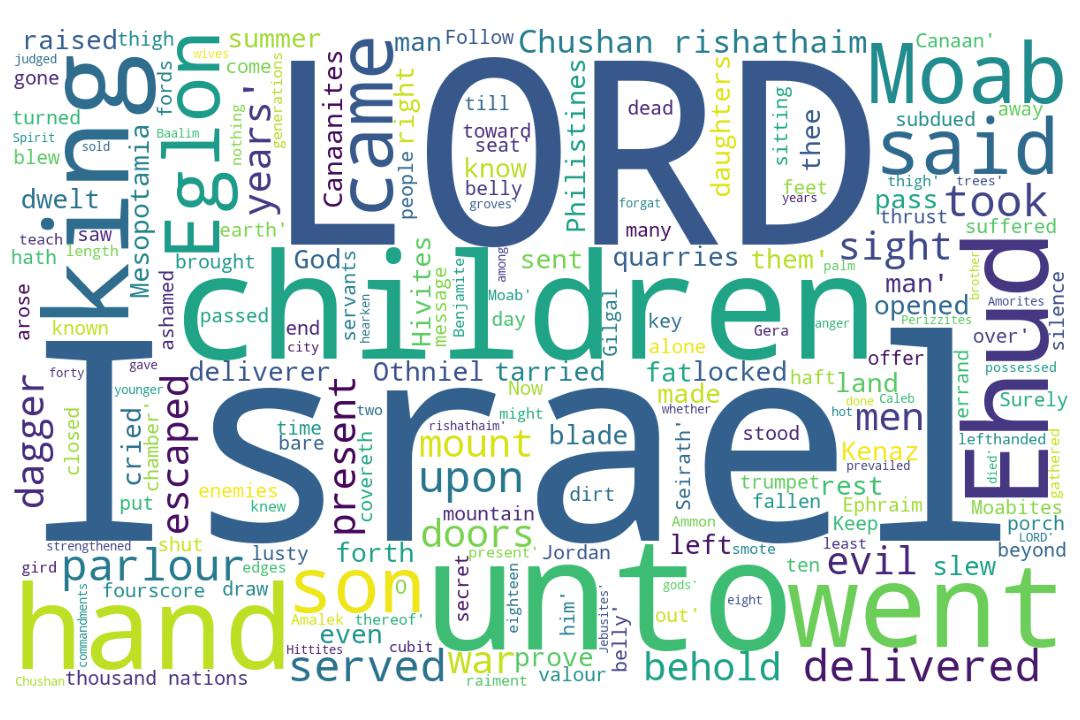
\includegraphics[width=\linewidth]{07OT-Judges/Judges3-WordCloud.jpg}
  \caption{Judges 3 Word Cloud}
  \label{fig:Judges 3 Word Cloud}
\end{figure}

\marginpar{\scriptsize \centering \fcolorbox{bone}{lime}{\textbf{A CYCLE APPEARS}}\\ (Judges 3:1-7) \begin{compactenum}[I.][8]
    \item   The \textbf{Thorns}  \index[scripture]{Judges!Jdg 03:01} (Jdg 3:1) 
    \item   The \textbf{Teaching}  \index[scripture]{Judges!Jdg 03:02} (Jdg 3:2) 
    \item    \textbf{Testing}  \index[scripture]{Judges!Jdg 03:04} (Jdg 3:4) 
    \item   A \textbf{Toxin}  \index[scripture]{Judges!Jdg 03:06} (Jdg 3:6) 
    \item   The \textbf{Transgressions}  \index[scripture]{Judges!Jdg 03:07} (Jdg 3:7) 
    \item   Ruined \textbf{Theology}  \index[scripture]{Judges!Jdg 03:07} (Jdg 3:7) 
    \item   The \textbf{Theme}  the cycle of sin, judgmentm repentance, rescue % \index[scripture]{Judges!Jdg 03:01} (Judges 3:1) 
\end{compactenum}}


\marginpar{\scriptsize \centering \fcolorbox{bone}{yellow}{\textbf{ROUND 1}}\\ (Judges 3:5-11) 
\begin{compactenum}[I.][8]
    \item   \textbf{Six} Enemies \index[scripture]{Judges!Jdg 03:05} (Jdg 3:5) 
    \item   \textbf{Sons \& Daughters}  \index[scripture]{Judges!Jdg 03:06} (Jdg 3:6)  
    \item   \textbf{Service} to Balaam \index[scripture]{Judges!Jdg 03:07} (Jdg 3:7)  
    \item   \textbf{Sold} to Mesopotamia \index[scripture]{Judges!Jdg 03:08} (Jdg 3:8)  
    \item   Israel's  \textbf{Supplication} \index[scripture]{Judges!Jdg 03:09} (Jdg 3:9)  
    \item   Othniel, the \textbf{Savior} \index[scripture]{Judges!Jdg 03:09} (Jdg 3:9)  
    \item   \textbf{Stillness} for 40 Years \index[scripture]{Judges!Jdg 03:11} (Jdg 3:11)  
\end{compactenum}}




\footnote{\textcolor[cmyk]{0.99998,1,0,0}{\hyperlink{TOC}{Return to end of Table of Contents.}}}\footnote{\href{https://audiobible.com/bible/judges_3.html}{\textcolor[cmyk]{0.99998,1,0,0}{Judges 3 Audio}}}\textcolor[cmyk]{0.99998,1,0,0}{Now these \emph{are} the nations which the LORD left, \fcolorbox{bone}{lime}{to prove} Israel by them, \emph{even} as many \emph{of} \emph{Israel} as had not known all the wars of Canaan;}
[2] \textcolor[cmyk]{0.99998,1,0,0}{Only that the generations of the children of Israel might \fcolorbox{bone}{lime}{know}, to teach them war, at the least such as before knew nothing thereof;}
[3] \textcolor[cmyk]{0.99998,1,0,0}{\emph{Namely}, five lords of the Philistines, and all the Canaanites, and the Sidonians, and the Hivites that dwelt in mount Lebanon, from mount Baal-hermon unto the entering in of Hamath.}
[4] \textcolor[cmyk]{0.99998,1,0,0}{And they were to \fcolorbox{bone}{lime}{prove} Israel by them, to know whether they would hearken unto the commandments of the LORD, which he commanded their fathers by the hand of Moses.}\\
\\
\P \textcolor[cmyk]{0.99998,1,0,0}{And the children of Israel dwelt among the \fcolorbox{bone}{yellow}{Canaanites}, \fcolorbox{bone}{yellow}{Hittites}, and \fcolorbox{bone}{yellow}{Amorites}, and \fcolorbox{bone}{yellow}{Perizzites}, and \fcolorbox{bone}{yellow}{Hivites}, and \fcolorbox{bone}{yellow}{Jebusites}:}
[6] \textcolor[cmyk]{0.99998,1,0,0}{And they took their \fcolorbox{bone}{lime}{daughters} to be their wives, and gave their daughters to their \fcolorbox{bone}{lime}{sons}, and served their gods.}
[7] \textcolor[cmyk]{0.99998,1,0,0}{And the children of Israel did \fcolorbox{bone}{lime}{evil} in the sight of the LORD, and \fcolorbox{bone}{lime}{forgat} the LORD their God, and \fcolorbox{bone}{lime}{served} Baalim and the groves.}\\
\\
\P \textcolor[cmyk]{0.99998,1,0,0}{Therefore the anger of the LORD was hot against Israel, and he sold them into the hand of Chushan-rishathaim king of Mesopotamia: and the children of Israel served Chushan-rishathaim eight years.}
[9] \textcolor[cmyk]{0.99998,1,0,0}{And when the children of Israel \fcolorbox{bone}{yellow}{cried} unto the LORD, the LORD raised up a deliverer to the children of Israel, who delivered them, \emph{even} \fcolorbox{bone}{yellow}{Othniel} the son of Kenaz, Caleb's younger brother.}
[10] \textcolor[cmyk]{0.99998,1,0,0}{And the Spirit of the LORD came upon him, and he judged Israel, and went out to war: and the LORD delivered Chushan-rishathaim king of Mesopotamia into his hand; and his hand prevailed against Chushan-rishathaim.}
[11] \textcolor[cmyk]{0.99998,1,0,0}{And the land had \fcolorbox{bone}{yellow}{rest} forty years. And Othniel the son of Kenaz died.}\\
\\
\P \textcolor[cmyk]{0.99998,1,0,0}{And the children of Israel did evil again in the sight of the LORD: and the LORD strengthened Eglon the king of Moab against Israel, because they had done evil in the sight of the LORD.}
[13] \textcolor[cmyk]{0.99998,1,0,0}{And he gathered unto him the children of Ammon and Amalek, and went and smote Israel, and possessed the city of palm trees.}
[14] \textcolor[cmyk]{0.99998,1,0,0}{So the children of Israel served Eglon the king of Moab eighteen years.}
[15] \textcolor[cmyk]{0.99998,1,0,0}{But when the children of Israel cried unto the LORD, the LORD raised them up a deliverer, Ehud the son of Gera, a Benjamite, a man lefthanded: and by him the children of Israel sent a present unto Eglon the king of Moab.}
[16] \textcolor[cmyk]{0.99998,1,0,0}{But Ehud made him a dagger which had two edges, of a cubit length; and he did gird it under his raiment upon his right thigh.}
[17] \textcolor[cmyk]{0.99998,1,0,0}{And he brought the present unto Eglon king of Moab: and Eglon \emph{was} a very fat man.}
[18] \textcolor[cmyk]{0.99998,1,0,0}{And when he had made an end to offer the present, he sent away the people that bare the present.}
[19] \textcolor[cmyk]{0.99998,1,0,0}{But he himself turned again from the quarries that \emph{were} by Gilgal, and said, I have a secret errand unto thee, O king: who said, Keep silence. And all that stood by him went out from him.}
[20] \textcolor[cmyk]{0.99998,1,0,0}{And Ehud came unto him; and he was sitting in a summer parlour, which he had for himself alone. And Ehud said, I have a message from God unto thee. And he arose out of \emph{his} seat.}
[21] \textcolor[cmyk]{0.99998,1,0,0}{And Ehud put forth his left hand, and took the dagger from his right thigh, and thrust it into his belly:}
[22] \textcolor[cmyk]{0.99998,1,0,0}{And the haft also went in after the blade; and the fat closed upon the blade, so that he could not draw the dagger out of his belly; and the dirt came out.}
[23] \textcolor[cmyk]{0.99998,1,0,0}{Then Ehud went forth through the porch, and shut the doors of the parlour upon him, and locked them.}
[24] \textcolor[cmyk]{0.99998,1,0,0}{When he was gone out, his servants came; and when they saw that, behold, the doors of the parlour \emph{were} locked, they said, Surely he covereth his feet in his summer chamber.}
[25] \textcolor[cmyk]{0.99998,1,0,0}{And they tarried till they were ashamed: and, behold, he opened not the doors of the parlour; therefore they took a key, and opened \emph{them}: and, behold, their lord \emph{was} fallen down dead on the earth.}
[26] \textcolor[cmyk]{0.99998,1,0,0}{And Ehud escaped while they tarried, and passed beyond the quarries, and escaped unto Seirath.}
[27] \textcolor[cmyk]{0.99998,1,0,0}{And it came to pass, when he was come, that he blew a trumpet in the mountain of Ephraim, and the children of Israel went down with him from the mount, and he before them.}
[28] \textcolor[cmyk]{0.99998,1,0,0}{And he said unto them, Follow after me: for the LORD hath delivered your enemies the Moabites into your hand. And they went down after him, and took the fords of Jordan toward Moab, and suffered not a man to pass over.}
[29] \textcolor[cmyk]{0.99998,1,0,0}{And they slew of Moab at that time about ten thousand men, all lusty, and all men of valour; and there escaped not a man.}
[30] \textcolor[cmyk]{0.99998,1,0,0}{So Moab was subdued that day under the hand of Israel. And the land had rest fourscore years.}\\
\\
\P \textcolor[cmyk]{0.99998,1,0,0}{And after him was Shamgar the son of Anath, which slew of the Philistines six hundred men with an ox goad: and he also delivered Israel.}
\index[NWIV]{28!Judges!Jud 3:1}\index[AWIP]{Now!Judges!Jud 3:1}\index[AWIP]{these!Judges!Jud 3:1}\index[AWIP]{\emph{are}!Judges!Jud 3:1}\index[AWIP]{the!Judges!Jud 3:1}\index[AWIP]{the!Judges!Jud 3:1 (2)}\index[AWIP]{the!Judges!Jud 3:1 (3)}\index[AWIP]{nations!Judges!Jud 3:1}\index[AWIP]{which!Judges!Jud 3:1}\index[AWIP]{LORD!Judges!Jud 3:1}\index[AWIP]{left!Judges!Jud 3:1}\index[AWIP]{to!Judges!Jud 3:1}\index[AWIP]{prove!Judges!Jud 3:1}\index[AWIP]{Israel!Judges!Jud 3:1}\index[AWIP]{by!Judges!Jud 3:1}\index[AWIP]{them!Judges!Jud 3:1}\index[AWIP]{\emph{even}!Judges!Jud 3:1}\index[AWIP]{as!Judges!Jud 3:1}\index[AWIP]{as!Judges!Jud 3:1 (2)}\index[AWIP]{many!Judges!Jud 3:1}\index[AWIP]{\emph{of}!Judges!Jud 3:1}\index[AWIP]{\emph{Israel}!Judges!Jud 3:1}\index[AWIP]{had!Judges!Jud 3:1}\index[AWIP]{not!Judges!Jud 3:1}\index[AWIP]{known!Judges!Jud 3:1}\index[AWIP]{all!Judges!Jud 3:1}\index[AWIP]{wars!Judges!Jud 3:1}\index[AWIP]{of!Judges!Jud 3:1}\index[AWIP]{Canaan!Judges!Jud 3:1}\index[AWIP]{\emph{are}!Judges!Jud 3:1}\index[AWIP]{\emph{even}!Judges!Jud 3:1}\index[AWIP]{\emph{of}!Judges!Jud 3:1}\index[AWIP]{\emph{Israel}!Judges!Jud 3:1}

\index[NWIV]{24!Judges!Jud 3:2}\index[AWIP]{Only!Judges!Jud 3:2}\index[AWIP]{that!Judges!Jud 3:2}\index[AWIP]{the!Judges!Jud 3:2}\index[AWIP]{the!Judges!Jud 3:2 (2)}\index[AWIP]{the!Judges!Jud 3:2 (3)}\index[AWIP]{generations!Judges!Jud 3:2}\index[AWIP]{of!Judges!Jud 3:2}\index[AWIP]{of!Judges!Jud 3:2 (2)}\index[AWIP]{children!Judges!Jud 3:2}\index[AWIP]{Israel!Judges!Jud 3:2}\index[AWIP]{might!Judges!Jud 3:2}\index[AWIP]{know!Judges!Jud 3:2}\index[AWIP]{to!Judges!Jud 3:2}\index[AWIP]{teach!Judges!Jud 3:2}\index[AWIP]{them!Judges!Jud 3:2}\index[AWIP]{war!Judges!Jud 3:2}\index[AWIP]{at!Judges!Jud 3:2}\index[AWIP]{least!Judges!Jud 3:2}\index[AWIP]{such!Judges!Jud 3:2}\index[AWIP]{as!Judges!Jud 3:2}\index[AWIP]{before!Judges!Jud 3:2}\index[AWIP]{knew!Judges!Jud 3:2}\index[AWIP]{nothing!Judges!Jud 3:2}\index[AWIP]{thereof!Judges!Jud 3:2}

\index[NWIV]{30!Judges!Jud 3:3}\index[AWIP]{\emph{Namely}!Judges!Jud 3:3}\index[AWIP]{five!Judges!Jud 3:3}\index[AWIP]{lords!Judges!Jud 3:3}\index[AWIP]{of!Judges!Jud 3:3}\index[AWIP]{of!Judges!Jud 3:3 (2)}\index[AWIP]{the!Judges!Jud 3:3}\index[AWIP]{the!Judges!Jud 3:3 (2)}\index[AWIP]{the!Judges!Jud 3:3 (3)}\index[AWIP]{the!Judges!Jud 3:3 (4)}\index[AWIP]{the!Judges!Jud 3:3 (5)}\index[AWIP]{Philistines!Judges!Jud 3:3}\index[AWIP]{and!Judges!Jud 3:3}\index[AWIP]{and!Judges!Jud 3:3 (2)}\index[AWIP]{and!Judges!Jud 3:3 (3)}\index[AWIP]{all!Judges!Jud 3:3}\index[AWIP]{Canaanites!Judges!Jud 3:3}\index[AWIP]{Sidonians!Judges!Jud 3:3}\index[AWIP]{Hivites!Judges!Jud 3:3}\index[AWIP]{that!Judges!Jud 3:3}\index[AWIP]{dwelt!Judges!Jud 3:3}\index[AWIP]{in!Judges!Jud 3:3}\index[AWIP]{in!Judges!Jud 3:3 (2)}\index[AWIP]{mount!Judges!Jud 3:3}\index[AWIP]{mount!Judges!Jud 3:3 (2)}\index[AWIP]{Lebanon!Judges!Jud 3:3}\index[AWIP]{from!Judges!Jud 3:3}\index[AWIP]{Baal-hermon!Judges!Jud 3:3}\index[AWIP]{unto!Judges!Jud 3:3}\index[AWIP]{entering!Judges!Jud 3:3}\index[AWIP]{Hamath!Judges!Jud 3:3}\index[AWIP]{\emph{Namely}!Judges!Jud 3:3}

\index[NWIV]{30!Judges!Jud 3:4}\index[AWIP]{And!Judges!Jud 3:4}\index[AWIP]{they!Judges!Jud 3:4}\index[AWIP]{they!Judges!Jud 3:4 (2)}\index[AWIP]{were!Judges!Jud 3:4}\index[AWIP]{to!Judges!Jud 3:4}\index[AWIP]{to!Judges!Jud 3:4 (2)}\index[AWIP]{prove!Judges!Jud 3:4}\index[AWIP]{Israel!Judges!Jud 3:4}\index[AWIP]{by!Judges!Jud 3:4}\index[AWIP]{by!Judges!Jud 3:4 (2)}\index[AWIP]{them!Judges!Jud 3:4}\index[AWIP]{know!Judges!Jud 3:4}\index[AWIP]{whether!Judges!Jud 3:4}\index[AWIP]{would!Judges!Jud 3:4}\index[AWIP]{hearken!Judges!Jud 3:4}\index[AWIP]{unto!Judges!Jud 3:4}\index[AWIP]{the!Judges!Jud 3:4}\index[AWIP]{the!Judges!Jud 3:4 (2)}\index[AWIP]{the!Judges!Jud 3:4 (3)}\index[AWIP]{commandments!Judges!Jud 3:4}\index[AWIP]{of!Judges!Jud 3:4}\index[AWIP]{of!Judges!Jud 3:4 (2)}\index[AWIP]{LORD!Judges!Jud 3:4}\index[AWIP]{which!Judges!Jud 3:4}\index[AWIP]{he!Judges!Jud 3:4}\index[AWIP]{commanded!Judges!Jud 3:4}\index[AWIP]{their!Judges!Jud 3:4}\index[AWIP]{fathers!Judges!Jud 3:4}\index[AWIP]{hand!Judges!Jud 3:4}\index[AWIP]{Moses!Judges!Jud 3:4}

\index[NWIV]{18!Judges!Jud 3:5}\index[AWIP]{And!Judges!Jud 3:5}\index[AWIP]{the!Judges!Jud 3:5}\index[AWIP]{the!Judges!Jud 3:5 (2)}\index[AWIP]{children!Judges!Jud 3:5}\index[AWIP]{of!Judges!Jud 3:5}\index[AWIP]{Israel!Judges!Jud 3:5}\index[AWIP]{dwelt!Judges!Jud 3:5}\index[AWIP]{among!Judges!Jud 3:5}\index[AWIP]{Canaanites!Judges!Jud 3:5}\index[AWIP]{Hittites!Judges!Jud 3:5}\index[AWIP]{and!Judges!Jud 3:5}\index[AWIP]{and!Judges!Jud 3:5 (2)}\index[AWIP]{and!Judges!Jud 3:5 (3)}\index[AWIP]{and!Judges!Jud 3:5 (4)}\index[AWIP]{Amorites!Judges!Jud 3:5}\index[AWIP]{Perizzites!Judges!Jud 3:5}\index[AWIP]{Hivites!Judges!Jud 3:5}\index[AWIP]{Jebusites!Judges!Jud 3:5}

\index[NWIV]{20!Judges!Jud 3:6}\index[AWIP]{And!Judges!Jud 3:6}\index[AWIP]{they!Judges!Jud 3:6}\index[AWIP]{took!Judges!Jud 3:6}\index[AWIP]{their!Judges!Jud 3:6}\index[AWIP]{their!Judges!Jud 3:6 (2)}\index[AWIP]{their!Judges!Jud 3:6 (3)}\index[AWIP]{their!Judges!Jud 3:6 (4)}\index[AWIP]{their!Judges!Jud 3:6 (5)}\index[AWIP]{daughters!Judges!Jud 3:6}\index[AWIP]{daughters!Judges!Jud 3:6 (2)}\index[AWIP]{to!Judges!Jud 3:6}\index[AWIP]{to!Judges!Jud 3:6 (2)}\index[AWIP]{be!Judges!Jud 3:6}\index[AWIP]{wives!Judges!Jud 3:6}\index[AWIP]{and!Judges!Jud 3:6}\index[AWIP]{and!Judges!Jud 3:6 (2)}\index[AWIP]{gave!Judges!Jud 3:6}\index[AWIP]{sons!Judges!Jud 3:6}\index[AWIP]{served!Judges!Jud 3:6}\index[AWIP]{gods!Judges!Jud 3:6}

\index[NWIV]{25!Judges!Jud 3:7}\index[AWIP]{And!Judges!Jud 3:7}\index[AWIP]{the!Judges!Jud 3:7}\index[AWIP]{the!Judges!Jud 3:7 (2)}\index[AWIP]{the!Judges!Jud 3:7 (3)}\index[AWIP]{the!Judges!Jud 3:7 (4)}\index[AWIP]{the!Judges!Jud 3:7 (5)}\index[AWIP]{children!Judges!Jud 3:7}\index[AWIP]{of!Judges!Jud 3:7}\index[AWIP]{of!Judges!Jud 3:7 (2)}\index[AWIP]{Israel!Judges!Jud 3:7}\index[AWIP]{did!Judges!Jud 3:7}\index[AWIP]{evil!Judges!Jud 3:7}\index[AWIP]{in!Judges!Jud 3:7}\index[AWIP]{sight!Judges!Jud 3:7}\index[AWIP]{LORD!Judges!Jud 3:7}\index[AWIP]{LORD!Judges!Jud 3:7 (2)}\index[AWIP]{and!Judges!Jud 3:7}\index[AWIP]{and!Judges!Jud 3:7 (2)}\index[AWIP]{and!Judges!Jud 3:7 (3)}\index[AWIP]{forgat!Judges!Jud 3:7}\index[AWIP]{their!Judges!Jud 3:7}\index[AWIP]{God!Judges!Jud 3:7}\index[AWIP]{served!Judges!Jud 3:7}\index[AWIP]{Baalim!Judges!Jud 3:7}\index[AWIP]{groves!Judges!Jud 3:7}

\index[NWIV]{31!Judges!Jud 3:8}\index[AWIP]{Therefore!Judges!Jud 3:8}\index[AWIP]{the!Judges!Jud 3:8}\index[AWIP]{the!Judges!Jud 3:8 (2)}\index[AWIP]{the!Judges!Jud 3:8 (3)}\index[AWIP]{the!Judges!Jud 3:8 (4)}\index[AWIP]{anger!Judges!Jud 3:8}\index[AWIP]{of!Judges!Jud 3:8}\index[AWIP]{of!Judges!Jud 3:8 (2)}\index[AWIP]{of!Judges!Jud 3:8 (3)}\index[AWIP]{of!Judges!Jud 3:8 (4)}\index[AWIP]{LORD!Judges!Jud 3:8}\index[AWIP]{was!Judges!Jud 3:8}\index[AWIP]{hot!Judges!Jud 3:8}\index[AWIP]{against!Judges!Jud 3:8}\index[AWIP]{Israel!Judges!Jud 3:8}\index[AWIP]{Israel!Judges!Jud 3:8 (2)}\index[AWIP]{and!Judges!Jud 3:8}\index[AWIP]{and!Judges!Jud 3:8 (2)}\index[AWIP]{he!Judges!Jud 3:8}\index[AWIP]{sold!Judges!Jud 3:8}\index[AWIP]{them!Judges!Jud 3:8}\index[AWIP]{into!Judges!Jud 3:8}\index[AWIP]{hand!Judges!Jud 3:8}\index[AWIP]{Chushan-rishathaim!Judges!Jud 3:8}\index[AWIP]{Chushan-rishathaim!Judges!Jud 3:8 (2)}\index[AWIP]{king!Judges!Jud 3:8}\index[AWIP]{Mesopotamia!Judges!Jud 3:8}\index[AWIP]{children!Judges!Jud 3:8}\index[AWIP]{served!Judges!Jud 3:8}\index[AWIP]{eight!Judges!Jud 3:8}\index[AWIP]{years!Judges!Jud 3:8}

\index[NWIV]{33!Judges!Jud 3:9}\index[AWIP]{And!Judges!Jud 3:9}\index[AWIP]{when!Judges!Jud 3:9}\index[AWIP]{the!Judges!Jud 3:9}\index[AWIP]{the!Judges!Jud 3:9 (2)}\index[AWIP]{the!Judges!Jud 3:9 (3)}\index[AWIP]{the!Judges!Jud 3:9 (4)}\index[AWIP]{the!Judges!Jud 3:9 (5)}\index[AWIP]{children!Judges!Jud 3:9}\index[AWIP]{children!Judges!Jud 3:9 (2)}\index[AWIP]{of!Judges!Jud 3:9}\index[AWIP]{of!Judges!Jud 3:9 (2)}\index[AWIP]{of!Judges!Jud 3:9 (3)}\index[AWIP]{Israel!Judges!Jud 3:9}\index[AWIP]{Israel!Judges!Jud 3:9 (2)}\index[AWIP]{cried!Judges!Jud 3:9}\index[AWIP]{unto!Judges!Jud 3:9}\index[AWIP]{LORD!Judges!Jud 3:9}\index[AWIP]{LORD!Judges!Jud 3:9 (2)}\index[AWIP]{raised!Judges!Jud 3:9}\index[AWIP]{up!Judges!Jud 3:9}\index[AWIP]{a!Judges!Jud 3:9}\index[AWIP]{deliverer!Judges!Jud 3:9}\index[AWIP]{to!Judges!Jud 3:9}\index[AWIP]{who!Judges!Jud 3:9}\index[AWIP]{delivered!Judges!Jud 3:9}\index[AWIP]{them!Judges!Jud 3:9}\index[AWIP]{\emph{even}!Judges!Jud 3:9}\index[AWIP]{Othniel!Judges!Jud 3:9}\index[AWIP]{son!Judges!Jud 3:9}\index[AWIP]{Kenaz!Judges!Jud 3:9}\index[AWIP]{Caleb's!Judges!Jud 3:9}\index[AWIP]{younger!Judges!Jud 3:9}\index[AWIP]{brother!Judges!Jud 3:9}\index[AWIP]{\emph{even}!Judges!Jud 3:9}

\index[NWIV]{35!Judges!Jud 3:10}\index[AWIP]{And!Judges!Jud 3:10}\index[AWIP]{the!Judges!Jud 3:10}\index[AWIP]{the!Judges!Jud 3:10 (2)}\index[AWIP]{the!Judges!Jud 3:10 (3)}\index[AWIP]{Spirit!Judges!Jud 3:10}\index[AWIP]{of!Judges!Jud 3:10}\index[AWIP]{of!Judges!Jud 3:10 (2)}\index[AWIP]{LORD!Judges!Jud 3:10}\index[AWIP]{LORD!Judges!Jud 3:10 (2)}\index[AWIP]{came!Judges!Jud 3:10}\index[AWIP]{upon!Judges!Jud 3:10}\index[AWIP]{him!Judges!Jud 3:10}\index[AWIP]{and!Judges!Jud 3:10}\index[AWIP]{and!Judges!Jud 3:10 (2)}\index[AWIP]{and!Judges!Jud 3:10 (3)}\index[AWIP]{and!Judges!Jud 3:10 (4)}\index[AWIP]{he!Judges!Jud 3:10}\index[AWIP]{judged!Judges!Jud 3:10}\index[AWIP]{Israel!Judges!Jud 3:10}\index[AWIP]{went!Judges!Jud 3:10}\index[AWIP]{out!Judges!Jud 3:10}\index[AWIP]{to!Judges!Jud 3:10}\index[AWIP]{war!Judges!Jud 3:10}\index[AWIP]{delivered!Judges!Jud 3:10}\index[AWIP]{Chushan-rishathaim!Judges!Jud 3:10}\index[AWIP]{Chushan-rishathaim!Judges!Jud 3:10 (2)}\index[AWIP]{king!Judges!Jud 3:10}\index[AWIP]{Mesopotamia!Judges!Jud 3:10}\index[AWIP]{into!Judges!Jud 3:10}\index[AWIP]{his!Judges!Jud 3:10}\index[AWIP]{his!Judges!Jud 3:10 (2)}\index[AWIP]{hand!Judges!Jud 3:10}\index[AWIP]{hand!Judges!Jud 3:10 (2)}\index[AWIP]{prevailed!Judges!Jud 3:10}\index[AWIP]{against!Judges!Jud 3:10}

\index[NWIV]{14!Judges!Jud 3:11}\index[AWIP]{And!Judges!Jud 3:11}\index[AWIP]{And!Judges!Jud 3:11 (2)}\index[AWIP]{the!Judges!Jud 3:11}\index[AWIP]{the!Judges!Jud 3:11 (2)}\index[AWIP]{land!Judges!Jud 3:11}\index[AWIP]{had!Judges!Jud 3:11}\index[AWIP]{rest!Judges!Jud 3:11}\index[AWIP]{forty!Judges!Jud 3:11}\index[AWIP]{years!Judges!Jud 3:11}\index[AWIP]{Othniel!Judges!Jud 3:11}\index[AWIP]{son!Judges!Jud 3:11}\index[AWIP]{of!Judges!Jud 3:11}\index[AWIP]{Kenaz!Judges!Jud 3:11}\index[AWIP]{died!Judges!Jud 3:11}

\index[NWIV]{36!Judges!Jud 3:12}\index[AWIP]{And!Judges!Jud 3:12}\index[AWIP]{the!Judges!Jud 3:12}\index[AWIP]{the!Judges!Jud 3:12 (2)}\index[AWIP]{the!Judges!Jud 3:12 (3)}\index[AWIP]{the!Judges!Jud 3:12 (4)}\index[AWIP]{the!Judges!Jud 3:12 (5)}\index[AWIP]{the!Judges!Jud 3:12 (6)}\index[AWIP]{the!Judges!Jud 3:12 (7)}\index[AWIP]{children!Judges!Jud 3:12}\index[AWIP]{of!Judges!Jud 3:12}\index[AWIP]{of!Judges!Jud 3:12 (2)}\index[AWIP]{of!Judges!Jud 3:12 (3)}\index[AWIP]{of!Judges!Jud 3:12 (4)}\index[AWIP]{Israel!Judges!Jud 3:12}\index[AWIP]{Israel!Judges!Jud 3:12 (2)}\index[AWIP]{did!Judges!Jud 3:12}\index[AWIP]{evil!Judges!Jud 3:12}\index[AWIP]{evil!Judges!Jud 3:12 (2)}\index[AWIP]{again!Judges!Jud 3:12}\index[AWIP]{in!Judges!Jud 3:12}\index[AWIP]{in!Judges!Jud 3:12 (2)}\index[AWIP]{sight!Judges!Jud 3:12}\index[AWIP]{sight!Judges!Jud 3:12 (2)}\index[AWIP]{LORD!Judges!Jud 3:12}\index[AWIP]{LORD!Judges!Jud 3:12 (2)}\index[AWIP]{LORD!Judges!Jud 3:12 (3)}\index[AWIP]{and!Judges!Jud 3:12}\index[AWIP]{strengthened!Judges!Jud 3:12}\index[AWIP]{Eglon!Judges!Jud 3:12}\index[AWIP]{king!Judges!Jud 3:12}\index[AWIP]{Moab!Judges!Jud 3:12}\index[AWIP]{against!Judges!Jud 3:12}\index[AWIP]{because!Judges!Jud 3:12}\index[AWIP]{they!Judges!Jud 3:12}\index[AWIP]{had!Judges!Jud 3:12}\index[AWIP]{done!Judges!Jud 3:12}

\index[NWIV]{23!Judges!Jud 3:13}\index[AWIP]{And!Judges!Jud 3:13}\index[AWIP]{he!Judges!Jud 3:13}\index[AWIP]{gathered!Judges!Jud 3:13}\index[AWIP]{unto!Judges!Jud 3:13}\index[AWIP]{him!Judges!Jud 3:13}\index[AWIP]{the!Judges!Jud 3:13}\index[AWIP]{the!Judges!Jud 3:13 (2)}\index[AWIP]{children!Judges!Jud 3:13}\index[AWIP]{of!Judges!Jud 3:13}\index[AWIP]{of!Judges!Jud 3:13 (2)}\index[AWIP]{Ammon!Judges!Jud 3:13}\index[AWIP]{and!Judges!Jud 3:13}\index[AWIP]{and!Judges!Jud 3:13 (2)}\index[AWIP]{and!Judges!Jud 3:13 (3)}\index[AWIP]{and!Judges!Jud 3:13 (4)}\index[AWIP]{Amalek!Judges!Jud 3:13}\index[AWIP]{went!Judges!Jud 3:13}\index[AWIP]{smote!Judges!Jud 3:13}\index[AWIP]{Israel!Judges!Jud 3:13}\index[AWIP]{possessed!Judges!Jud 3:13}\index[AWIP]{city!Judges!Jud 3:13}\index[AWIP]{palm!Judges!Jud 3:13}\index[AWIP]{trees!Judges!Jud 3:13}

\index[NWIV]{13!Judges!Jud 3:14}\index[AWIP]{So!Judges!Jud 3:14}\index[AWIP]{the!Judges!Jud 3:14}\index[AWIP]{the!Judges!Jud 3:14 (2)}\index[AWIP]{children!Judges!Jud 3:14}\index[AWIP]{of!Judges!Jud 3:14}\index[AWIP]{of!Judges!Jud 3:14 (2)}\index[AWIP]{Israel!Judges!Jud 3:14}\index[AWIP]{served!Judges!Jud 3:14}\index[AWIP]{Eglon!Judges!Jud 3:14}\index[AWIP]{king!Judges!Jud 3:14}\index[AWIP]{Moab!Judges!Jud 3:14}\index[AWIP]{eighteen!Judges!Jud 3:14}\index[AWIP]{years!Judges!Jud 3:14}

\index[NWIV]{43!Judges!Jud 3:15}\index[AWIP]{But!Judges!Jud 3:15}\index[AWIP]{when!Judges!Jud 3:15}\index[AWIP]{the!Judges!Jud 3:15}\index[AWIP]{the!Judges!Jud 3:15 (2)}\index[AWIP]{the!Judges!Jud 3:15 (3)}\index[AWIP]{the!Judges!Jud 3:15 (4)}\index[AWIP]{the!Judges!Jud 3:15 (5)}\index[AWIP]{the!Judges!Jud 3:15 (6)}\index[AWIP]{children!Judges!Jud 3:15}\index[AWIP]{children!Judges!Jud 3:15 (2)}\index[AWIP]{of!Judges!Jud 3:15}\index[AWIP]{of!Judges!Jud 3:15 (2)}\index[AWIP]{of!Judges!Jud 3:15 (3)}\index[AWIP]{of!Judges!Jud 3:15 (4)}\index[AWIP]{Israel!Judges!Jud 3:15}\index[AWIP]{Israel!Judges!Jud 3:15 (2)}\index[AWIP]{cried!Judges!Jud 3:15}\index[AWIP]{unto!Judges!Jud 3:15}\index[AWIP]{unto!Judges!Jud 3:15 (2)}\index[AWIP]{LORD!Judges!Jud 3:15}\index[AWIP]{LORD!Judges!Jud 3:15 (2)}\index[AWIP]{raised!Judges!Jud 3:15}\index[AWIP]{them!Judges!Jud 3:15}\index[AWIP]{up!Judges!Jud 3:15}\index[AWIP]{a!Judges!Jud 3:15}\index[AWIP]{a!Judges!Jud 3:15 (2)}\index[AWIP]{a!Judges!Jud 3:15 (3)}\index[AWIP]{a!Judges!Jud 3:15 (4)}\index[AWIP]{deliverer!Judges!Jud 3:15}\index[AWIP]{Ehud!Judges!Jud 3:15}\index[AWIP]{son!Judges!Jud 3:15}\index[AWIP]{Gera!Judges!Jud 3:15}\index[AWIP]{Benjamite!Judges!Jud 3:15}\index[AWIP]{man!Judges!Jud 3:15}\index[AWIP]{lefthanded!Judges!Jud 3:15}\index[AWIP]{and!Judges!Jud 3:15}\index[AWIP]{by!Judges!Jud 3:15}\index[AWIP]{him!Judges!Jud 3:15}\index[AWIP]{sent!Judges!Jud 3:15}\index[AWIP]{present!Judges!Jud 3:15}\index[AWIP]{Eglon!Judges!Jud 3:15}\index[AWIP]{king!Judges!Jud 3:15}\index[AWIP]{Moab!Judges!Jud 3:15}

\index[NWIV]{26!Judges!Jud 3:16}\index[AWIP]{But!Judges!Jud 3:16}\index[AWIP]{Ehud!Judges!Jud 3:16}\index[AWIP]{made!Judges!Jud 3:16}\index[AWIP]{him!Judges!Jud 3:16}\index[AWIP]{a!Judges!Jud 3:16}\index[AWIP]{a!Judges!Jud 3:16 (2)}\index[AWIP]{dagger!Judges!Jud 3:16}\index[AWIP]{which!Judges!Jud 3:16}\index[AWIP]{had!Judges!Jud 3:16}\index[AWIP]{two!Judges!Jud 3:16}\index[AWIP]{edges!Judges!Jud 3:16}\index[AWIP]{of!Judges!Jud 3:16}\index[AWIP]{cubit!Judges!Jud 3:16}\index[AWIP]{length!Judges!Jud 3:16}\index[AWIP]{and!Judges!Jud 3:16}\index[AWIP]{he!Judges!Jud 3:16}\index[AWIP]{did!Judges!Jud 3:16}\index[AWIP]{gird!Judges!Jud 3:16}\index[AWIP]{it!Judges!Jud 3:16}\index[AWIP]{under!Judges!Jud 3:16}\index[AWIP]{his!Judges!Jud 3:16}\index[AWIP]{his!Judges!Jud 3:16 (2)}\index[AWIP]{raiment!Judges!Jud 3:16}\index[AWIP]{upon!Judges!Jud 3:16}\index[AWIP]{right!Judges!Jud 3:16}\index[AWIP]{thigh!Judges!Jud 3:16}

\index[NWIV]{17!Judges!Jud 3:17}\index[AWIP]{And!Judges!Jud 3:17}\index[AWIP]{he!Judges!Jud 3:17}\index[AWIP]{brought!Judges!Jud 3:17}\index[AWIP]{the!Judges!Jud 3:17}\index[AWIP]{present!Judges!Jud 3:17}\index[AWIP]{unto!Judges!Jud 3:17}\index[AWIP]{Eglon!Judges!Jud 3:17}\index[AWIP]{Eglon!Judges!Jud 3:17 (2)}\index[AWIP]{king!Judges!Jud 3:17}\index[AWIP]{of!Judges!Jud 3:17}\index[AWIP]{Moab!Judges!Jud 3:17}\index[AWIP]{and!Judges!Jud 3:17}\index[AWIP]{\emph{was}!Judges!Jud 3:17}\index[AWIP]{a!Judges!Jud 3:17}\index[AWIP]{very!Judges!Jud 3:17}\index[AWIP]{fat!Judges!Jud 3:17}\index[AWIP]{man!Judges!Jud 3:17}\index[AWIP]{\emph{was}!Judges!Jud 3:17}

\index[NWIV]{20!Judges!Jud 3:18}\index[AWIP]{And!Judges!Jud 3:18}\index[AWIP]{when!Judges!Jud 3:18}\index[AWIP]{he!Judges!Jud 3:18}\index[AWIP]{he!Judges!Jud 3:18 (2)}\index[AWIP]{had!Judges!Jud 3:18}\index[AWIP]{made!Judges!Jud 3:18}\index[AWIP]{an!Judges!Jud 3:18}\index[AWIP]{end!Judges!Jud 3:18}\index[AWIP]{to!Judges!Jud 3:18}\index[AWIP]{offer!Judges!Jud 3:18}\index[AWIP]{the!Judges!Jud 3:18}\index[AWIP]{the!Judges!Jud 3:18 (2)}\index[AWIP]{the!Judges!Jud 3:18 (3)}\index[AWIP]{present!Judges!Jud 3:18}\index[AWIP]{present!Judges!Jud 3:18 (2)}\index[AWIP]{sent!Judges!Jud 3:18}\index[AWIP]{away!Judges!Jud 3:18}\index[AWIP]{people!Judges!Jud 3:18}\index[AWIP]{that!Judges!Jud 3:18}\index[AWIP]{bare!Judges!Jud 3:18}

\index[NWIV]{37!Judges!Jud 3:19}\index[AWIP]{But!Judges!Jud 3:19}\index[AWIP]{he!Judges!Jud 3:19}\index[AWIP]{himself!Judges!Jud 3:19}\index[AWIP]{turned!Judges!Jud 3:19}\index[AWIP]{again!Judges!Jud 3:19}\index[AWIP]{from!Judges!Jud 3:19}\index[AWIP]{from!Judges!Jud 3:19 (2)}\index[AWIP]{the!Judges!Jud 3:19}\index[AWIP]{quarries!Judges!Jud 3:19}\index[AWIP]{that!Judges!Jud 3:19}\index[AWIP]{that!Judges!Jud 3:19 (2)}\index[AWIP]{\emph{were}!Judges!Jud 3:19}\index[AWIP]{by!Judges!Jud 3:19}\index[AWIP]{by!Judges!Jud 3:19 (2)}\index[AWIP]{Gilgal!Judges!Jud 3:19}\index[AWIP]{and!Judges!Jud 3:19}\index[AWIP]{said!Judges!Jud 3:19}\index[AWIP]{said!Judges!Jud 3:19 (2)}\index[AWIP]{I!Judges!Jud 3:19}\index[AWIP]{have!Judges!Jud 3:19}\index[AWIP]{a!Judges!Jud 3:19}\index[AWIP]{secret!Judges!Jud 3:19}\index[AWIP]{errand!Judges!Jud 3:19}\index[AWIP]{unto!Judges!Jud 3:19}\index[AWIP]{thee!Judges!Jud 3:19}\index[AWIP]{O!Judges!Jud 3:19}\index[AWIP]{king!Judges!Jud 3:19}\index[AWIP]{who!Judges!Jud 3:19}\index[AWIP]{Keep!Judges!Jud 3:19}\index[AWIP]{silence!Judges!Jud 3:19}\index[AWIP]{And!Judges!Jud 3:19}\index[AWIP]{all!Judges!Jud 3:19}\index[AWIP]{stood!Judges!Jud 3:19}\index[AWIP]{him!Judges!Jud 3:19}\index[AWIP]{him!Judges!Jud 3:19 (2)}\index[AWIP]{went!Judges!Jud 3:19}\index[AWIP]{out!Judges!Jud 3:19}\index[AWIP]{\emph{were}!Judges!Jud 3:19}

\index[NWIV]{37!Judges!Jud 3:20}\index[AWIP]{And!Judges!Jud 3:20}\index[AWIP]{And!Judges!Jud 3:20 (2)}\index[AWIP]{And!Judges!Jud 3:20 (3)}\index[AWIP]{Ehud!Judges!Jud 3:20}\index[AWIP]{Ehud!Judges!Jud 3:20 (2)}\index[AWIP]{came!Judges!Jud 3:20}\index[AWIP]{unto!Judges!Jud 3:20}\index[AWIP]{unto!Judges!Jud 3:20 (2)}\index[AWIP]{him!Judges!Jud 3:20}\index[AWIP]{and!Judges!Jud 3:20}\index[AWIP]{he!Judges!Jud 3:20}\index[AWIP]{he!Judges!Jud 3:20 (2)}\index[AWIP]{he!Judges!Jud 3:20 (3)}\index[AWIP]{was!Judges!Jud 3:20}\index[AWIP]{sitting!Judges!Jud 3:20}\index[AWIP]{in!Judges!Jud 3:20}\index[AWIP]{a!Judges!Jud 3:20}\index[AWIP]{a!Judges!Jud 3:20 (2)}\index[AWIP]{summer!Judges!Jud 3:20}\index[AWIP]{parlour!Judges!Jud 3:20}\index[AWIP]{which!Judges!Jud 3:20}\index[AWIP]{had!Judges!Jud 3:20}\index[AWIP]{for!Judges!Jud 3:20}\index[AWIP]{himself!Judges!Jud 3:20}\index[AWIP]{alone!Judges!Jud 3:20}\index[AWIP]{said!Judges!Jud 3:20}\index[AWIP]{I!Judges!Jud 3:20}\index[AWIP]{have!Judges!Jud 3:20}\index[AWIP]{message!Judges!Jud 3:20}\index[AWIP]{from!Judges!Jud 3:20}\index[AWIP]{God!Judges!Jud 3:20}\index[AWIP]{thee!Judges!Jud 3:20}\index[AWIP]{arose!Judges!Jud 3:20}\index[AWIP]{out!Judges!Jud 3:20}\index[AWIP]{of!Judges!Jud 3:20}\index[AWIP]{\emph{his}!Judges!Jud 3:20}\index[AWIP]{seat!Judges!Jud 3:20}\index[AWIP]{\emph{his}!Judges!Jud 3:20}

\index[NWIV]{21!Judges!Jud 3:21}\index[AWIP]{And!Judges!Jud 3:21}\index[AWIP]{Ehud!Judges!Jud 3:21}\index[AWIP]{put!Judges!Jud 3:21}\index[AWIP]{forth!Judges!Jud 3:21}\index[AWIP]{his!Judges!Jud 3:21}\index[AWIP]{his!Judges!Jud 3:21 (2)}\index[AWIP]{his!Judges!Jud 3:21 (3)}\index[AWIP]{left!Judges!Jud 3:21}\index[AWIP]{hand!Judges!Jud 3:21}\index[AWIP]{and!Judges!Jud 3:21}\index[AWIP]{and!Judges!Jud 3:21 (2)}\index[AWIP]{took!Judges!Jud 3:21}\index[AWIP]{the!Judges!Jud 3:21}\index[AWIP]{dagger!Judges!Jud 3:21}\index[AWIP]{from!Judges!Jud 3:21}\index[AWIP]{right!Judges!Jud 3:21}\index[AWIP]{thigh!Judges!Jud 3:21}\index[AWIP]{thrust!Judges!Jud 3:21}\index[AWIP]{it!Judges!Jud 3:21}\index[AWIP]{into!Judges!Jud 3:21}\index[AWIP]{belly!Judges!Jud 3:21}

\index[NWIV]{33!Judges!Jud 3:22}\index[AWIP]{And!Judges!Jud 3:22}\index[AWIP]{the!Judges!Jud 3:22}\index[AWIP]{the!Judges!Jud 3:22 (2)}\index[AWIP]{the!Judges!Jud 3:22 (3)}\index[AWIP]{the!Judges!Jud 3:22 (4)}\index[AWIP]{the!Judges!Jud 3:22 (5)}\index[AWIP]{the!Judges!Jud 3:22 (6)}\index[AWIP]{haft!Judges!Jud 3:22}\index[AWIP]{also!Judges!Jud 3:22}\index[AWIP]{went!Judges!Jud 3:22}\index[AWIP]{in!Judges!Jud 3:22}\index[AWIP]{after!Judges!Jud 3:22}\index[AWIP]{blade!Judges!Jud 3:22}\index[AWIP]{blade!Judges!Jud 3:22 (2)}\index[AWIP]{and!Judges!Jud 3:22}\index[AWIP]{and!Judges!Jud 3:22 (2)}\index[AWIP]{fat!Judges!Jud 3:22}\index[AWIP]{closed!Judges!Jud 3:22}\index[AWIP]{upon!Judges!Jud 3:22}\index[AWIP]{so!Judges!Jud 3:22}\index[AWIP]{that!Judges!Jud 3:22}\index[AWIP]{he!Judges!Jud 3:22}\index[AWIP]{could!Judges!Jud 3:22}\index[AWIP]{not!Judges!Jud 3:22}\index[AWIP]{draw!Judges!Jud 3:22}\index[AWIP]{dagger!Judges!Jud 3:22}\index[AWIP]{out!Judges!Jud 3:22}\index[AWIP]{out!Judges!Jud 3:22 (2)}\index[AWIP]{of!Judges!Jud 3:22}\index[AWIP]{his!Judges!Jud 3:22}\index[AWIP]{belly!Judges!Jud 3:22}\index[AWIP]{dirt!Judges!Jud 3:22}\index[AWIP]{came!Judges!Jud 3:22}

\index[NWIV]{19!Judges!Jud 3:23}\index[AWIP]{Then!Judges!Jud 3:23}\index[AWIP]{Ehud!Judges!Jud 3:23}\index[AWIP]{went!Judges!Jud 3:23}\index[AWIP]{forth!Judges!Jud 3:23}\index[AWIP]{through!Judges!Jud 3:23}\index[AWIP]{the!Judges!Jud 3:23}\index[AWIP]{the!Judges!Jud 3:23 (2)}\index[AWIP]{the!Judges!Jud 3:23 (3)}\index[AWIP]{porch!Judges!Jud 3:23}\index[AWIP]{and!Judges!Jud 3:23}\index[AWIP]{and!Judges!Jud 3:23 (2)}\index[AWIP]{shut!Judges!Jud 3:23}\index[AWIP]{doors!Judges!Jud 3:23}\index[AWIP]{of!Judges!Jud 3:23}\index[AWIP]{parlour!Judges!Jud 3:23}\index[AWIP]{upon!Judges!Jud 3:23}\index[AWIP]{him!Judges!Jud 3:23}\index[AWIP]{locked!Judges!Jud 3:23}\index[AWIP]{them!Judges!Jud 3:23}

\index[NWIV]{32!Judges!Jud 3:24}\index[AWIP]{When!Judges!Jud 3:24}\index[AWIP]{he!Judges!Jud 3:24}\index[AWIP]{he!Judges!Jud 3:24 (2)}\index[AWIP]{was!Judges!Jud 3:24}\index[AWIP]{gone!Judges!Jud 3:24}\index[AWIP]{out!Judges!Jud 3:24}\index[AWIP]{his!Judges!Jud 3:24}\index[AWIP]{his!Judges!Jud 3:24 (2)}\index[AWIP]{his!Judges!Jud 3:24 (3)}\index[AWIP]{servants!Judges!Jud 3:24}\index[AWIP]{came!Judges!Jud 3:24}\index[AWIP]{and!Judges!Jud 3:24}\index[AWIP]{when!Judges!Jud 3:24}\index[AWIP]{they!Judges!Jud 3:24}\index[AWIP]{they!Judges!Jud 3:24 (2)}\index[AWIP]{saw!Judges!Jud 3:24}\index[AWIP]{that!Judges!Jud 3:24}\index[AWIP]{behold!Judges!Jud 3:24}\index[AWIP]{the!Judges!Jud 3:24}\index[AWIP]{the!Judges!Jud 3:24 (2)}\index[AWIP]{doors!Judges!Jud 3:24}\index[AWIP]{of!Judges!Jud 3:24}\index[AWIP]{parlour!Judges!Jud 3:24}\index[AWIP]{\emph{were}!Judges!Jud 3:24}\index[AWIP]{locked!Judges!Jud 3:24}\index[AWIP]{said!Judges!Jud 3:24}\index[AWIP]{Surely!Judges!Jud 3:24}\index[AWIP]{covereth!Judges!Jud 3:24}\index[AWIP]{feet!Judges!Jud 3:24}\index[AWIP]{in!Judges!Jud 3:24}\index[AWIP]{summer!Judges!Jud 3:24}\index[AWIP]{chamber!Judges!Jud 3:24}\index[AWIP]{\emph{were}!Judges!Jud 3:24}

\index[NWIV]{36!Judges!Jud 3:25}\index[AWIP]{And!Judges!Jud 3:25}\index[AWIP]{they!Judges!Jud 3:25}\index[AWIP]{they!Judges!Jud 3:25 (2)}\index[AWIP]{they!Judges!Jud 3:25 (3)}\index[AWIP]{tarried!Judges!Jud 3:25}\index[AWIP]{till!Judges!Jud 3:25}\index[AWIP]{were!Judges!Jud 3:25}\index[AWIP]{ashamed!Judges!Jud 3:25}\index[AWIP]{and!Judges!Jud 3:25}\index[AWIP]{and!Judges!Jud 3:25 (2)}\index[AWIP]{and!Judges!Jud 3:25 (3)}\index[AWIP]{behold!Judges!Jud 3:25}\index[AWIP]{behold!Judges!Jud 3:25 (2)}\index[AWIP]{he!Judges!Jud 3:25}\index[AWIP]{opened!Judges!Jud 3:25}\index[AWIP]{opened!Judges!Jud 3:25 (2)}\index[AWIP]{not!Judges!Jud 3:25}\index[AWIP]{the!Judges!Jud 3:25}\index[AWIP]{the!Judges!Jud 3:25 (2)}\index[AWIP]{the!Judges!Jud 3:25 (3)}\index[AWIP]{doors!Judges!Jud 3:25}\index[AWIP]{of!Judges!Jud 3:25}\index[AWIP]{parlour!Judges!Jud 3:25}\index[AWIP]{therefore!Judges!Jud 3:25}\index[AWIP]{took!Judges!Jud 3:25}\index[AWIP]{a!Judges!Jud 3:25}\index[AWIP]{key!Judges!Jud 3:25}\index[AWIP]{\emph{them}!Judges!Jud 3:25}\index[AWIP]{their!Judges!Jud 3:25}\index[AWIP]{lord!Judges!Jud 3:25}\index[AWIP]{\emph{was}!Judges!Jud 3:25}\index[AWIP]{fallen!Judges!Jud 3:25}\index[AWIP]{down!Judges!Jud 3:25}\index[AWIP]{dead!Judges!Jud 3:25}\index[AWIP]{on!Judges!Jud 3:25}\index[AWIP]{earth!Judges!Jud 3:25}\index[AWIP]{\emph{them}!Judges!Jud 3:25}\index[AWIP]{\emph{was}!Judges!Jud 3:25}

\index[NWIV]{15!Judges!Jud 3:26}\index[AWIP]{And!Judges!Jud 3:26}\index[AWIP]{Ehud!Judges!Jud 3:26}\index[AWIP]{escaped!Judges!Jud 3:26}\index[AWIP]{escaped!Judges!Jud 3:26 (2)}\index[AWIP]{while!Judges!Jud 3:26}\index[AWIP]{they!Judges!Jud 3:26}\index[AWIP]{tarried!Judges!Jud 3:26}\index[AWIP]{and!Judges!Jud 3:26}\index[AWIP]{and!Judges!Jud 3:26 (2)}\index[AWIP]{passed!Judges!Jud 3:26}\index[AWIP]{beyond!Judges!Jud 3:26}\index[AWIP]{the!Judges!Jud 3:26}\index[AWIP]{quarries!Judges!Jud 3:26}\index[AWIP]{unto!Judges!Jud 3:26}\index[AWIP]{Seirath!Judges!Jud 3:26}

\index[NWIV]{35!Judges!Jud 3:27}\index[AWIP]{And!Judges!Jud 3:27}\index[AWIP]{it!Judges!Jud 3:27}\index[AWIP]{came!Judges!Jud 3:27}\index[AWIP]{to!Judges!Jud 3:27}\index[AWIP]{pass!Judges!Jud 3:27}\index[AWIP]{when!Judges!Jud 3:27}\index[AWIP]{he!Judges!Jud 3:27}\index[AWIP]{he!Judges!Jud 3:27 (2)}\index[AWIP]{he!Judges!Jud 3:27 (3)}\index[AWIP]{was!Judges!Jud 3:27}\index[AWIP]{come!Judges!Jud 3:27}\index[AWIP]{that!Judges!Jud 3:27}\index[AWIP]{blew!Judges!Jud 3:27}\index[AWIP]{a!Judges!Jud 3:27}\index[AWIP]{trumpet!Judges!Jud 3:27}\index[AWIP]{in!Judges!Jud 3:27}\index[AWIP]{the!Judges!Jud 3:27}\index[AWIP]{the!Judges!Jud 3:27 (2)}\index[AWIP]{the!Judges!Jud 3:27 (3)}\index[AWIP]{mountain!Judges!Jud 3:27}\index[AWIP]{of!Judges!Jud 3:27}\index[AWIP]{of!Judges!Jud 3:27 (2)}\index[AWIP]{Ephraim!Judges!Jud 3:27}\index[AWIP]{and!Judges!Jud 3:27}\index[AWIP]{and!Judges!Jud 3:27 (2)}\index[AWIP]{children!Judges!Jud 3:27}\index[AWIP]{Israel!Judges!Jud 3:27}\index[AWIP]{went!Judges!Jud 3:27}\index[AWIP]{down!Judges!Jud 3:27}\index[AWIP]{with!Judges!Jud 3:27}\index[AWIP]{him!Judges!Jud 3:27}\index[AWIP]{from!Judges!Jud 3:27}\index[AWIP]{mount!Judges!Jud 3:27}\index[AWIP]{before!Judges!Jud 3:27}\index[AWIP]{them!Judges!Jud 3:27}

\index[NWIV]{42!Judges!Jud 3:28}\index[AWIP]{And!Judges!Jud 3:28}\index[AWIP]{And!Judges!Jud 3:28 (2)}\index[AWIP]{he!Judges!Jud 3:28}\index[AWIP]{said!Judges!Jud 3:28}\index[AWIP]{unto!Judges!Jud 3:28}\index[AWIP]{them!Judges!Jud 3:28}\index[AWIP]{Follow!Judges!Jud 3:28}\index[AWIP]{after!Judges!Jud 3:28}\index[AWIP]{after!Judges!Jud 3:28 (2)}\index[AWIP]{me!Judges!Jud 3:28}\index[AWIP]{for!Judges!Jud 3:28}\index[AWIP]{the!Judges!Jud 3:28}\index[AWIP]{the!Judges!Jud 3:28 (2)}\index[AWIP]{the!Judges!Jud 3:28 (3)}\index[AWIP]{LORD!Judges!Jud 3:28}\index[AWIP]{hath!Judges!Jud 3:28}\index[AWIP]{delivered!Judges!Jud 3:28}\index[AWIP]{your!Judges!Jud 3:28}\index[AWIP]{your!Judges!Jud 3:28 (2)}\index[AWIP]{enemies!Judges!Jud 3:28}\index[AWIP]{Moabites!Judges!Jud 3:28}\index[AWIP]{into!Judges!Jud 3:28}\index[AWIP]{hand!Judges!Jud 3:28}\index[AWIP]{they!Judges!Jud 3:28}\index[AWIP]{went!Judges!Jud 3:28}\index[AWIP]{down!Judges!Jud 3:28}\index[AWIP]{him!Judges!Jud 3:28}\index[AWIP]{and!Judges!Jud 3:28}\index[AWIP]{and!Judges!Jud 3:28 (2)}\index[AWIP]{took!Judges!Jud 3:28}\index[AWIP]{fords!Judges!Jud 3:28}\index[AWIP]{of!Judges!Jud 3:28}\index[AWIP]{Jordan!Judges!Jud 3:28}\index[AWIP]{toward!Judges!Jud 3:28}\index[AWIP]{Moab!Judges!Jud 3:28}\index[AWIP]{suffered!Judges!Jud 3:28}\index[AWIP]{not!Judges!Jud 3:28}\index[AWIP]{a!Judges!Jud 3:28}\index[AWIP]{man!Judges!Jud 3:28}\index[AWIP]{to!Judges!Jud 3:28}\index[AWIP]{pass!Judges!Jud 3:28}\index[AWIP]{over!Judges!Jud 3:28}

\index[NWIV]{25!Judges!Jud 3:29}\index[AWIP]{And!Judges!Jud 3:29}\index[AWIP]{they!Judges!Jud 3:29}\index[AWIP]{slew!Judges!Jud 3:29}\index[AWIP]{of!Judges!Jud 3:29}\index[AWIP]{of!Judges!Jud 3:29 (2)}\index[AWIP]{Moab!Judges!Jud 3:29}\index[AWIP]{at!Judges!Jud 3:29}\index[AWIP]{that!Judges!Jud 3:29}\index[AWIP]{time!Judges!Jud 3:29}\index[AWIP]{about!Judges!Jud 3:29}\index[AWIP]{ten!Judges!Jud 3:29}\index[AWIP]{thousand!Judges!Jud 3:29}\index[AWIP]{men!Judges!Jud 3:29}\index[AWIP]{men!Judges!Jud 3:29 (2)}\index[AWIP]{all!Judges!Jud 3:29}\index[AWIP]{all!Judges!Jud 3:29 (2)}\index[AWIP]{lusty!Judges!Jud 3:29}\index[AWIP]{and!Judges!Jud 3:29}\index[AWIP]{and!Judges!Jud 3:29 (2)}\index[AWIP]{valour!Judges!Jud 3:29}\index[AWIP]{there!Judges!Jud 3:29}\index[AWIP]{escaped!Judges!Jud 3:29}\index[AWIP]{not!Judges!Jud 3:29}\index[AWIP]{a!Judges!Jud 3:29}\index[AWIP]{man!Judges!Jud 3:29}

\index[NWIV]{18!Judges!Jud 3:30}\index[AWIP]{So!Judges!Jud 3:30}\index[AWIP]{Moab!Judges!Jud 3:30}\index[AWIP]{was!Judges!Jud 3:30}\index[AWIP]{subdued!Judges!Jud 3:30}\index[AWIP]{that!Judges!Jud 3:30}\index[AWIP]{day!Judges!Jud 3:30}\index[AWIP]{under!Judges!Jud 3:30}\index[AWIP]{the!Judges!Jud 3:30}\index[AWIP]{the!Judges!Jud 3:30 (2)}\index[AWIP]{hand!Judges!Jud 3:30}\index[AWIP]{of!Judges!Jud 3:30}\index[AWIP]{Israel!Judges!Jud 3:30}\index[AWIP]{And!Judges!Jud 3:30}\index[AWIP]{land!Judges!Jud 3:30}\index[AWIP]{had!Judges!Jud 3:30}\index[AWIP]{rest!Judges!Jud 3:30}\index[AWIP]{fourscore!Judges!Jud 3:30}\index[AWIP]{years!Judges!Jud 3:30}

\index[NWIV]{26!Judges!Jud 3:31}\index[AWIP]{And!Judges!Jud 3:31}\index[AWIP]{after!Judges!Jud 3:31}\index[AWIP]{him!Judges!Jud 3:31}\index[AWIP]{was!Judges!Jud 3:31}\index[AWIP]{Shamgar!Judges!Jud 3:31}\index[AWIP]{the!Judges!Jud 3:31}\index[AWIP]{the!Judges!Jud 3:31 (2)}\index[AWIP]{son!Judges!Jud 3:31}\index[AWIP]{of!Judges!Jud 3:31}\index[AWIP]{of!Judges!Jud 3:31 (2)}\index[AWIP]{Anath!Judges!Jud 3:31}\index[AWIP]{which!Judges!Jud 3:31}\index[AWIP]{slew!Judges!Jud 3:31}\index[AWIP]{Philistines!Judges!Jud 3:31}\index[AWIP]{six!Judges!Jud 3:31}\index[AWIP]{hundred!Judges!Jud 3:31}\index[AWIP]{men!Judges!Jud 3:31}\index[AWIP]{with!Judges!Jud 3:31}\index[AWIP]{an!Judges!Jud 3:31}\index[AWIP]{ox!Judges!Jud 3:31}\index[AWIP]{goad!Judges!Jud 3:31}\index[AWIP]{and!Judges!Jud 3:31}\index[AWIP]{he!Judges!Jud 3:31}\index[AWIP]{also!Judges!Jud 3:31}\index[AWIP]{delivered!Judges!Jud 3:31}\index[AWIP]{Israel!Judges!Jud 3:31}


\section{Judges 3 Outlines}

\subsection{My Outlines}

\subsubsection{A Cycle Appears}
\index[speaker]{Keith Anthony!Judges 03 (A Cycle Appears) }
\index[series]{Judges (Keith Anthony)!Judges 03 (A Cycle Appears) }
\index[date]{2018/03/15!Judges 03 (A Cycle Appears) (Keith Anthony)}
\begin{compactenum}[I.][8]
    \item   The \textbf{Thorns}  \index[scripture]{Judges!Jdg 03:01} (Jdg 3:1) 
    \item   The \textbf{Teaching}  \index[scripture]{Judges!Jdg 03:02} (Jdg 3:2) 
    \item    \textbf{Testing}  \index[scripture]{Judges!Jdg 03:04} (Jdg 3:4) 
    \item   A \textbf{Toxin}  \index[scripture]{Judges!Jdg 03:06} (Jdg 3:6) 
    \item   The \textbf{Transgressions}  \index[scripture]{Judges!Jdg 03:07} (Jdg 3:7) 
    \item   Ruined \textbf{Theology}  \index[scripture]{Judges!Jdg 03:07} (Jdg 3:7) 
    \item   The \textbf{Theme}  the cycle of sin, judgmentm repentance, rescue % \index[scripture]{Judges!Jdg 03:01} (Judges 3:1) 
\end{compactenum}


\subsubsection{Round 1}
\index[speaker]{Keith Anthony!Judges 03 (Round 1) }
\index[series]{Judges (Keith Anthony)!Judges 03 (Round 1) }
\index[date]{2020/03/14!Judges 03 (Round 1) (Keith Anthony)}
\begin{compactenum}[I.][8]
    \item   \textbf{Six} Enemies \index[scripture]{Judges!Jdg 03:05} (Jdg 3:5) 
    \item   \textbf{Sons \& Daughters}  \index[scripture]{Judges!Jdg 03:06} (Jdg 3:6)  
    \item   \textbf{Service} to Balaam \index[scripture]{Judges!Jdg 03:07} (Jdg 3:7)  
    \item   \textbf{Sold} to Mesopotamia \index[scripture]{Judges!Jdg 03:08} (Jdg 3:8)  
    \item   Israel's  \textbf{Supplication} \index[scripture]{Judges!Jdg 03:09} (Jdg 3:6)  
    \item   Othniel, the \textbf{Savior} \index[scripture]{Judges!Jdg 03:09} (Jdg 3:6)  
    \item   \textbf{Stillness} for 40 Years \index[scripture]{Judges!Jdg 03:11} (Jdg 3:11)  
\end{compactenum}

\subsection{Outlines from Others}
\section{Judges 3 Comments}

\subsection{Numeric Nuggets}
\textbf{13: } Verse 14 has 13 words.
\subsection{Judges 3 Repeated Phrases}


%%%%%%%%%%
%%%%%%%%%%
\normalsize
 
\begin{center}
\begin{longtable}{|p{3.0in}|p{0.5in}|}
\caption[Judges 3 Repeated Phrases]{Judges 3 Repeated Phrases}\label{table:Repeated Phrases Judges 3} \\
\hline \multicolumn{1}{|c|}{\textbf{Phrase}} & \multicolumn{1}{c|}{\textbf{Frequency}} \\ \hline 
\endfirsthead
 
\multicolumn{2}{c}
{{\bfseries \tablename\ \thetable{} -- continued from previous page}} \\  
\hline \multicolumn{1}{|c|}{\textbf{Phrase}} & \multicolumn{1}{c|}{\textbf{Frequency}} \\ \hline 
\endhead
 
\hline \multicolumn{2}{c}{{ }} \\ \hline
\endfoot 
the LORD & 15\\ \hline 
of the & 12\\ \hline 
the children & 12\\ \hline 
the children of & 12\\ \hline 
children of & 12\\ \hline 
of Israel & 12\\ \hline 
the children of Israel & 11\\ \hline 
children of Israel & 11\\ \hline 
and the & 9\\ \hline 
And the & 7\\ \hline 
of the LORD & 6\\ \hline 
and he & 6\\ \hline 
king of & 6\\ \hline 
And they & 5\\ \hline 
of Moab & 5\\ \hline 
unto the & 4\\ \hline 
in the & 4\\ \hline 
the son & 4\\ \hline 
the son of & 4\\ \hline 
son of & 4\\ \hline 
him and & 4\\ \hline 
king of Moab & 4\\ \hline 
And he & 4\\ \hline 
And Ehud & 4\\ \hline 
the hand & 3\\ \hline 
the hand of & 3\\ \hline 
hand of & 3\\ \hline 
And the children & 3\\ \hline 
And the children of & 3\\ \hline 
And the children of Israel & 3\\ \hline 
in the sight & 3\\ \hline 
in the sight of & 3\\ \hline 
in the sight of the & 3\\ \hline 
in the sight of the LORD & 3\\ \hline 
the sight & 3\\ \hline 
the sight of & 3\\ \hline 
the sight of the & 3\\ \hline 
the sight of the LORD & 3\\ \hline 
sight of & 3\\ \hline 
sight of the & 3\\ \hline 
sight of the LORD & 3\\ \hline 
Israel and & 3\\ \hline 
Eglon the & 3\\ \hline 
Eglon the king & 3\\ \hline 
Eglon the king of & 3\\ \hline 
Eglon the king of Moab & 3\\ \hline 
the king & 3\\ \hline 
the king of & 3\\ \hline 
the king of Moab & 3\\ \hline 
a man & 3\\ \hline 
the present & 3\\ \hline 
he was & 3\\ \hline 
the doors & 3\\ \hline 
the doors of & 3\\ \hline 
the doors of the & 3\\ \hline 
the doors of the parlour & 3\\ \hline 
doors of & 3\\ \hline 
doors of the & 3\\ \hline 
doors of the parlour & 3\\ \hline 
of the parlour & 3\\ \hline 
the parlour & 3\\ \hline 
\end{longtable}
\end{center}



%%%%%%%%%%
%%%%%%%%%%



\section{Judges 3 Statistics}

%%%%%%%%%%%%%%%%%%%%%%%%%%%
%%%%% Word Statistics
%%%%%%%%%%%%%%%%%%%%%%%%%%


\normalsize



\subsection{Chapter Word Statistics}


%%%%%%%%%%
%%%%%%%%%%
 
\begin{center}
\begin{longtable}{l|c|c|c|c}
\caption[Stats for Judges 3]{Stats for Judges 3} \label{table:Stats for Judges 3} \\ 
\hline \multicolumn{1}{|c|}{\textbf{Verse(s)}} & \multicolumn{1}{|c|}{\textbf{Count}} & \multicolumn{1}{|c|}{\textbf{Unique}} & \multicolumn{1}{|c|}{\textbf{Italics}} & \multicolumn{1}{|c|}{\textbf{Uniq Italic}}  \\ \hline 
\endfirsthead
 
\multicolumn{5}{c}
{{\bfseries \tablename\ \thetable{} -- continued from previous page}} \\  
\hline \multicolumn{1}{|c|}{\textbf{Verse(s)}} & \multicolumn{1}{|c|}{\textbf{Count}} & \multicolumn{1}{|c|}{\textbf{Unique}} & \multicolumn{1}{|c|}{\textbf{Italics}} & \multicolumn{1}{|c|}{\textbf{Uniq Italic}}  \\ \hline 
\endhead
 
\hline \multicolumn{5}{|r|}{{Continued if needed}} \\ \hline
\endfoot 
1 & 28 & 25 & 4 & 4\\ \hline
2 & 24 & 21 & 0 & 0\\ \hline
3 & 30 & 21 & 1 & 1\\ \hline
4 & 30 & 24 & 0 & 0\\ \hline
5 & 18 & 14 & 0 & 0\\ \hline
6 & 20 & 13 & 0 & 0\\ \hline
7 & 25 & 17 & 0 & 0\\ \hline
8 & 31 & 22 & 0 & 0\\ \hline
9 & 33 & 24 & 1 & 1\\ \hline
10 & 35 & 25 & 0 & 0\\ \hline
11 & 14 & 12 & 0 & 0\\ \hline
12 & 36 & 21 & 0 & 0\\ \hline
13 & 23 & 18 & 0 & 0\\ \hline
14 & 13 & 11 & 0 & 0\\ \hline
15 & 43 & 28 & 0 & 0\\ \hline
16 & 26 & 24 & 0 & 0\\ \hline
17 & 17 & 16 & 1 & 1\\ \hline
18 & 20 & 16 & 0 & 0\\ \hline
19 & 37 & 32 & 1 & 1\\ \hline
20 & 37 & 30 & 1 & 1\\ \hline
21 & 21 & 18 & 0 & 0\\ \hline
22 & 33 & 25 & 0 & 0\\ \hline
23 & 19 & 16 & 0 & 0\\ \hline
24 & 32 & 27 & 1 & 1\\ \hline
25 & 36 & 28 & 2 & 2\\ \hline
26 & 15 & 13 & 0 & 0\\ \hline
27 & 35 & 29 & 0 & 0\\ \hline
28 & 42 & 36 & 0 & 0\\ \hline
29 & 25 & 21 & 0 & 0\\ \hline
30 & 18 & 17 & 0 & 0\\ \hline
31 & 26 & 24 & 0 & 0\\ \hline
\hline \hline
Total & 842 & 281 & 12 & 9



\end{longtable}
\end{center}

%%%%%%%%%%
%%%%%%%%%%
 
\subsection{Words by Frequency}

\begin{center}
\begin{longtable}{l|r}
\caption[Word Frequencies in Judges 3]{Word Frequencies in Judges 3} \label{table:WordsIn-Judges-3} \\ 
\hline \multicolumn{1}{|c|}{\textbf{Word}} & \multicolumn{1}{c|}{\textbf{Frequency}} \\ \hline 
\endfirsthead
 
\multicolumn{2}{c}
{{\bfseries \tablename\ \thetable{} -- continued from previous page}} \\ 
\hline \multicolumn{1}{|c|}{\textbf{Word}} & \multicolumn{1}{c|}{\textbf{Frequency}} \\ \hline 
\endhead
 
\hline \multicolumn{2}{|r|}{{Continued if needed}} \\ \hline
\endfoot
 
\hline \hline
\endlastfoot
the & 83 \\ \hline
of & 47 \\ \hline
and & 47 \\ \hline
And & 26 \\ \hline
he & 21 \\ \hline
Israel & 19 \\ \hline
LORD & 15 \\ \hline
a & 15 \\ \hline
children & 12 \\ \hline
unto & 12 \\ \hline
they & 12 \\ \hline
to & 11 \\ \hline
him & 11 \\ \hline
his & 11 \\ \hline
that & 10 \\ \hline
them & 9 \\ \hline
in & 9 \\ \hline
their & 8 \\ \hline
had & 7 \\ \hline
hand & 7 \\ \hline
king & 7 \\ \hline
went & 7 \\ \hline
Moab & 7 \\ \hline
Ehud & 7 \\ \hline
by & 6 \\ \hline
from & 6 \\ \hline
was & 6 \\ \hline
out & 6 \\ \hline
which & 5 \\ \hline
not & 5 \\ \hline
all & 5 \\ \hline
when & 5 \\ \hline
came & 5 \\ \hline
Eglon & 5 \\ \hline
said & 5 \\ \hline
took & 4 \\ \hline
served & 4 \\ \hline
into & 4 \\ \hline
Chushan-rishathaim & 4 \\ \hline
years & 4 \\ \hline
delivered & 4 \\ \hline
son & 4 \\ \hline
upon & 4 \\ \hline
man & 4 \\ \hline
present & 4 \\ \hline
parlour & 4 \\ \hline
after & 4 \\ \hline
as & 3 \\ \hline
mount & 3 \\ \hline
did & 3 \\ \hline
evil & 3 \\ \hline
sight & 3 \\ \hline
against & 3 \\ \hline
But & 3 \\ \hline
dagger & 3 \\ \hline
it & 3 \\ \hline
doors & 3 \\ \hline
behold & 3 \\ \hline
down & 3 \\ \hline
escaped & 3 \\ \hline
men & 3 \\ \hline
left & 2 \\ \hline
prove & 2 \\ \hline
\emph{even} & 2 \\ \hline
know & 2 \\ \hline
war & 2 \\ \hline
at & 2 \\ \hline
before & 2 \\ \hline
Philistines & 2 \\ \hline
Canaanites & 2 \\ \hline
Hivites & 2 \\ \hline
dwelt & 2 \\ \hline
were & 2 \\ \hline
daughters & 2 \\ \hline
God & 2 \\ \hline
Mesopotamia & 2 \\ \hline
cried & 2 \\ \hline
raised & 2 \\ \hline
up & 2 \\ \hline
deliverer & 2 \\ \hline
who & 2 \\ \hline
Othniel & 2 \\ \hline
Kenaz & 2 \\ \hline
land & 2 \\ \hline
rest & 2 \\ \hline
again & 2 \\ \hline
So & 2 \\ \hline
sent & 2 \\ \hline
made & 2 \\ \hline
under & 2 \\ \hline
right & 2 \\ \hline
thigh & 2 \\ \hline
\emph{was} & 2 \\ \hline
fat & 2 \\ \hline
an & 2 \\ \hline
himself & 2 \\ \hline
quarries & 2 \\ \hline
\emph{were} & 2 \\ \hline
I & 2 \\ \hline
have & 2 \\ \hline
thee & 2 \\ \hline
summer & 2 \\ \hline
for & 2 \\ \hline
forth & 2 \\ \hline
belly & 2 \\ \hline
also & 2 \\ \hline
blade & 2 \\ \hline
locked & 2 \\ \hline
tarried & 2 \\ \hline
opened & 2 \\ \hline
pass & 2 \\ \hline
with & 2 \\ \hline
your & 2 \\ \hline
slew & 2 \\ \hline
Now & 1 \\ \hline
these & 1 \\ \hline
\emph{are} & 1 \\ \hline
nations & 1 \\ \hline
many & 1 \\ \hline
\emph{of} & 1 \\ \hline
\emph{Israel} & 1 \\ \hline
known & 1 \\ \hline
wars & 1 \\ \hline
Canaan & 1 \\ \hline
Only & 1 \\ \hline
generations & 1 \\ \hline
might & 1 \\ \hline
teach & 1 \\ \hline
least & 1 \\ \hline
such & 1 \\ \hline
knew & 1 \\ \hline
nothing & 1 \\ \hline
thereof & 1 \\ \hline
\emph{Namely} & 1 \\ \hline
five & 1 \\ \hline
lords & 1 \\ \hline
Sidonians & 1 \\ \hline
Lebanon & 1 \\ \hline
Baal-hermon & 1 \\ \hline
entering & 1 \\ \hline
Hamath & 1 \\ \hline
whether & 1 \\ \hline
would & 1 \\ \hline
hearken & 1 \\ \hline
commandments & 1 \\ \hline
commanded & 1 \\ \hline
fathers & 1 \\ \hline
Moses & 1 \\ \hline
among & 1 \\ \hline
Hittites & 1 \\ \hline
Amorites & 1 \\ \hline
Perizzites & 1 \\ \hline
Jebusites & 1 \\ \hline
be & 1 \\ \hline
wives & 1 \\ \hline
gave & 1 \\ \hline
sons & 1 \\ \hline
gods & 1 \\ \hline
forgat & 1 \\ \hline
Baalim & 1 \\ \hline
groves & 1 \\ \hline
Therefore & 1 \\ \hline
anger & 1 \\ \hline
hot & 1 \\ \hline
sold & 1 \\ \hline
eight & 1 \\ \hline
Caleb's & 1 \\ \hline
younger & 1 \\ \hline
brother & 1 \\ \hline
Spirit & 1 \\ \hline
judged & 1 \\ \hline
prevailed & 1 \\ \hline
forty & 1 \\ \hline
died & 1 \\ \hline
strengthened & 1 \\ \hline
because & 1 \\ \hline
done & 1 \\ \hline
gathered & 1 \\ \hline
Ammon & 1 \\ \hline
Amalek & 1 \\ \hline
smote & 1 \\ \hline
possessed & 1 \\ \hline
city & 1 \\ \hline
palm & 1 \\ \hline
trees & 1 \\ \hline
eighteen & 1 \\ \hline
Gera & 1 \\ \hline
Benjamite & 1 \\ \hline
lefthanded & 1 \\ \hline
two & 1 \\ \hline
edges & 1 \\ \hline
cubit & 1 \\ \hline
length & 1 \\ \hline
gird & 1 \\ \hline
raiment & 1 \\ \hline
brought & 1 \\ \hline
very & 1 \\ \hline
end & 1 \\ \hline
offer & 1 \\ \hline
away & 1 \\ \hline
people & 1 \\ \hline
bare & 1 \\ \hline
turned & 1 \\ \hline
Gilgal & 1 \\ \hline
secret & 1 \\ \hline
errand & 1 \\ \hline
O & 1 \\ \hline
Keep & 1 \\ \hline
silence & 1 \\ \hline
stood & 1 \\ \hline
sitting & 1 \\ \hline
alone & 1 \\ \hline
message & 1 \\ \hline
arose & 1 \\ \hline
\emph{his} & 1 \\ \hline
seat & 1 \\ \hline
put & 1 \\ \hline
thrust & 1 \\ \hline
haft & 1 \\ \hline
closed & 1 \\ \hline
so & 1 \\ \hline
could & 1 \\ \hline
draw & 1 \\ \hline
dirt & 1 \\ \hline
Then & 1 \\ \hline
through & 1 \\ \hline
porch & 1 \\ \hline
shut & 1 \\ \hline
When & 1 \\ \hline
gone & 1 \\ \hline
servants & 1 \\ \hline
saw & 1 \\ \hline
Surely & 1 \\ \hline
covereth & 1 \\ \hline
feet & 1 \\ \hline
chamber & 1 \\ \hline
till & 1 \\ \hline
ashamed & 1 \\ \hline
therefore & 1 \\ \hline
key & 1 \\ \hline
\emph{them} & 1 \\ \hline
lord & 1 \\ \hline
fallen & 1 \\ \hline
dead & 1 \\ \hline
on & 1 \\ \hline
earth & 1 \\ \hline
while & 1 \\ \hline
passed & 1 \\ \hline
beyond & 1 \\ \hline
Seirath & 1 \\ \hline
come & 1 \\ \hline
blew & 1 \\ \hline
trumpet & 1 \\ \hline
mountain & 1 \\ \hline
Ephraim & 1 \\ \hline
Follow & 1 \\ \hline
me & 1 \\ \hline
hath & 1 \\ \hline
enemies & 1 \\ \hline
Moabites & 1 \\ \hline
fords & 1 \\ \hline
Jordan & 1 \\ \hline
toward & 1 \\ \hline
suffered & 1 \\ \hline
over & 1 \\ \hline
time & 1 \\ \hline
about & 1 \\ \hline
ten & 1 \\ \hline
thousand & 1 \\ \hline
lusty & 1 \\ \hline
valour & 1 \\ \hline
there & 1 \\ \hline
subdued & 1 \\ \hline
day & 1 \\ \hline
fourscore & 1 \\ \hline
Shamgar & 1 \\ \hline
Anath & 1 \\ \hline
six & 1 \\ \hline
hundred & 1 \\ \hline
ox & 1 \\ \hline
goad & 1 \\ \hline
\end{longtable}
\end{center}



\normalsize



\subsection{Words Alphabetically}

\begin{center}
\begin{longtable}{l|r}
\caption[Word Alphabetically in Judges 3]{Word Alphabetically in Judges 3} \label{table:WordsIn-Judges-3} \\ 
\hline \multicolumn{1}{|c|}{\textbf{Word}} & \multicolumn{1}{c|}{\textbf{Frequency}} \\ \hline 
\endfirsthead
 
\multicolumn{2}{c}
{{\bfseries \tablename\ \thetable{} -- continued from previous page}} \\ 
\hline \multicolumn{1}{|c|}{\textbf{Word}} & \multicolumn{1}{c|}{\textbf{Frequency}} \\ \hline 
\endhead
 
\hline \multicolumn{2}{|r|}{{Continued if needed}} \\ \hline
\endfoot
 
\hline \hline
\endlastfoot
Amalek & 1 \\ \hline
Ammon & 1 \\ \hline
Amorites & 1 \\ \hline
Anath & 1 \\ \hline
And & 26 \\ \hline
Baal-hermon & 1 \\ \hline
Baalim & 1 \\ \hline
Benjamite & 1 \\ \hline
But & 3 \\ \hline
Caleb's & 1 \\ \hline
Canaan & 1 \\ \hline
Canaanites & 2 \\ \hline
Chushan-rishathaim & 4 \\ \hline
Eglon & 5 \\ \hline
Ehud & 7 \\ \hline
Ephraim & 1 \\ \hline
Follow & 1 \\ \hline
Gera & 1 \\ \hline
Gilgal & 1 \\ \hline
God & 2 \\ \hline
Hamath & 1 \\ \hline
Hittites & 1 \\ \hline
Hivites & 2 \\ \hline
I & 2 \\ \hline
Israel & 19 \\ \hline
Jebusites & 1 \\ \hline
Jordan & 1 \\ \hline
Keep & 1 \\ \hline
Kenaz & 2 \\ \hline
LORD & 15 \\ \hline
Lebanon & 1 \\ \hline
Mesopotamia & 2 \\ \hline
Moab & 7 \\ \hline
Moabites & 1 \\ \hline
Moses & 1 \\ \hline
Now & 1 \\ \hline
O & 1 \\ \hline
Only & 1 \\ \hline
Othniel & 2 \\ \hline
Perizzites & 1 \\ \hline
Philistines & 2 \\ \hline
Seirath & 1 \\ \hline
Shamgar & 1 \\ \hline
Sidonians & 1 \\ \hline
So & 2 \\ \hline
Spirit & 1 \\ \hline
Surely & 1 \\ \hline
Then & 1 \\ \hline
Therefore & 1 \\ \hline
When & 1 \\ \hline
\emph{Israel} & 1 \\ \hline
\emph{Namely} & 1 \\ \hline
\emph{are} & 1 \\ \hline
\emph{even} & 2 \\ \hline
\emph{his} & 1 \\ \hline
\emph{of} & 1 \\ \hline
\emph{them} & 1 \\ \hline
\emph{was} & 2 \\ \hline
\emph{were} & 2 \\ \hline
a & 15 \\ \hline
about & 1 \\ \hline
after & 4 \\ \hline
again & 2 \\ \hline
against & 3 \\ \hline
all & 5 \\ \hline
alone & 1 \\ \hline
also & 2 \\ \hline
among & 1 \\ \hline
an & 2 \\ \hline
and & 47 \\ \hline
anger & 1 \\ \hline
arose & 1 \\ \hline
as & 3 \\ \hline
ashamed & 1 \\ \hline
at & 2 \\ \hline
away & 1 \\ \hline
bare & 1 \\ \hline
be & 1 \\ \hline
because & 1 \\ \hline
before & 2 \\ \hline
behold & 3 \\ \hline
belly & 2 \\ \hline
beyond & 1 \\ \hline
blade & 2 \\ \hline
blew & 1 \\ \hline
brother & 1 \\ \hline
brought & 1 \\ \hline
by & 6 \\ \hline
came & 5 \\ \hline
chamber & 1 \\ \hline
children & 12 \\ \hline
city & 1 \\ \hline
closed & 1 \\ \hline
come & 1 \\ \hline
commanded & 1 \\ \hline
commandments & 1 \\ \hline
could & 1 \\ \hline
covereth & 1 \\ \hline
cried & 2 \\ \hline
cubit & 1 \\ \hline
dagger & 3 \\ \hline
daughters & 2 \\ \hline
day & 1 \\ \hline
dead & 1 \\ \hline
delivered & 4 \\ \hline
deliverer & 2 \\ \hline
did & 3 \\ \hline
died & 1 \\ \hline
dirt & 1 \\ \hline
done & 1 \\ \hline
doors & 3 \\ \hline
down & 3 \\ \hline
draw & 1 \\ \hline
dwelt & 2 \\ \hline
earth & 1 \\ \hline
edges & 1 \\ \hline
eight & 1 \\ \hline
eighteen & 1 \\ \hline
end & 1 \\ \hline
enemies & 1 \\ \hline
entering & 1 \\ \hline
errand & 1 \\ \hline
escaped & 3 \\ \hline
evil & 3 \\ \hline
fallen & 1 \\ \hline
fat & 2 \\ \hline
fathers & 1 \\ \hline
feet & 1 \\ \hline
five & 1 \\ \hline
for & 2 \\ \hline
fords & 1 \\ \hline
forgat & 1 \\ \hline
forth & 2 \\ \hline
forty & 1 \\ \hline
fourscore & 1 \\ \hline
from & 6 \\ \hline
gathered & 1 \\ \hline
gave & 1 \\ \hline
generations & 1 \\ \hline
gird & 1 \\ \hline
goad & 1 \\ \hline
gods & 1 \\ \hline
gone & 1 \\ \hline
groves & 1 \\ \hline
had & 7 \\ \hline
haft & 1 \\ \hline
hand & 7 \\ \hline
hath & 1 \\ \hline
have & 2 \\ \hline
he & 21 \\ \hline
hearken & 1 \\ \hline
him & 11 \\ \hline
himself & 2 \\ \hline
his & 11 \\ \hline
hot & 1 \\ \hline
hundred & 1 \\ \hline
in & 9 \\ \hline
into & 4 \\ \hline
it & 3 \\ \hline
judged & 1 \\ \hline
key & 1 \\ \hline
king & 7 \\ \hline
knew & 1 \\ \hline
know & 2 \\ \hline
known & 1 \\ \hline
land & 2 \\ \hline
least & 1 \\ \hline
left & 2 \\ \hline
lefthanded & 1 \\ \hline
length & 1 \\ \hline
locked & 2 \\ \hline
lord & 1 \\ \hline
lords & 1 \\ \hline
lusty & 1 \\ \hline
made & 2 \\ \hline
man & 4 \\ \hline
many & 1 \\ \hline
me & 1 \\ \hline
men & 3 \\ \hline
message & 1 \\ \hline
might & 1 \\ \hline
mount & 3 \\ \hline
mountain & 1 \\ \hline
nations & 1 \\ \hline
not & 5 \\ \hline
nothing & 1 \\ \hline
of & 47 \\ \hline
offer & 1 \\ \hline
on & 1 \\ \hline
opened & 2 \\ \hline
out & 6 \\ \hline
over & 1 \\ \hline
ox & 1 \\ \hline
palm & 1 \\ \hline
parlour & 4 \\ \hline
pass & 2 \\ \hline
passed & 1 \\ \hline
people & 1 \\ \hline
porch & 1 \\ \hline
possessed & 1 \\ \hline
present & 4 \\ \hline
prevailed & 1 \\ \hline
prove & 2 \\ \hline
put & 1 \\ \hline
quarries & 2 \\ \hline
raiment & 1 \\ \hline
raised & 2 \\ \hline
rest & 2 \\ \hline
right & 2 \\ \hline
said & 5 \\ \hline
saw & 1 \\ \hline
seat & 1 \\ \hline
secret & 1 \\ \hline
sent & 2 \\ \hline
servants & 1 \\ \hline
served & 4 \\ \hline
shut & 1 \\ \hline
sight & 3 \\ \hline
silence & 1 \\ \hline
sitting & 1 \\ \hline
six & 1 \\ \hline
slew & 2 \\ \hline
smote & 1 \\ \hline
so & 1 \\ \hline
sold & 1 \\ \hline
son & 4 \\ \hline
sons & 1 \\ \hline
stood & 1 \\ \hline
strengthened & 1 \\ \hline
subdued & 1 \\ \hline
such & 1 \\ \hline
suffered & 1 \\ \hline
summer & 2 \\ \hline
tarried & 2 \\ \hline
teach & 1 \\ \hline
ten & 1 \\ \hline
that & 10 \\ \hline
the & 83 \\ \hline
thee & 2 \\ \hline
their & 8 \\ \hline
them & 9 \\ \hline
there & 1 \\ \hline
therefore & 1 \\ \hline
thereof & 1 \\ \hline
these & 1 \\ \hline
they & 12 \\ \hline
thigh & 2 \\ \hline
thousand & 1 \\ \hline
through & 1 \\ \hline
thrust & 1 \\ \hline
till & 1 \\ \hline
time & 1 \\ \hline
to & 11 \\ \hline
took & 4 \\ \hline
toward & 1 \\ \hline
trees & 1 \\ \hline
trumpet & 1 \\ \hline
turned & 1 \\ \hline
two & 1 \\ \hline
under & 2 \\ \hline
unto & 12 \\ \hline
up & 2 \\ \hline
upon & 4 \\ \hline
valour & 1 \\ \hline
very & 1 \\ \hline
war & 2 \\ \hline
wars & 1 \\ \hline
was & 6 \\ \hline
went & 7 \\ \hline
were & 2 \\ \hline
when & 5 \\ \hline
whether & 1 \\ \hline
which & 5 \\ \hline
while & 1 \\ \hline
who & 2 \\ \hline
with & 2 \\ \hline
wives & 1 \\ \hline
would & 1 \\ \hline
years & 4 \\ \hline
younger & 1 \\ \hline
your & 2 \\ \hline
\end{longtable}
\end{center}



\normalsize



\subsection{Word Lengths in Chapter}
\normalsize
\begin{longtable}{l|p{3.75in}}
\caption[Words by Length in Judges 3]{Words by Length in Judges 3} \label{table:WordsIn-Judges-3} \\ 
\hline \multicolumn{1}{|c|}{\textbf{Length}} & \multicolumn{1}{c|}{\textbf{Words}} \\ \hline 
\endfirsthead
 
\multicolumn{2}{c}
{{\bfseries \tablename\ \thetable{} -- continued from previous page}} \\ 
\hline \multicolumn{1}{|c|}{\textbf{Length}} & \multicolumn{1}{c|}{\textbf{Words}} \\ \hline 
\endhead
 
\hline \multicolumn{2}{|r|}{{Continued if needed}} \\ \hline
\endfoot
 
\hline \hline
\endlastfoot
1 & a, I, O \\ \hline
2 & to, by, as, \emph{of}, of, at, in, he, be, up, So, it, an, so, on, me, ox \\ \hline
3 & Now, \emph{are}, the, had, not, all, war, and, And, did, God, was, hot, who, son, him, out, his, But, man, two, \emph{was}, fat, end, for, \emph{his}, put, saw, key, ten, men, day, six \\ \hline
4 & LORD, left, them, \emph{even}, many, wars, Only, that, know, such, knew, five, from, unto, they, were, hand, took, gave, sons, gods, evil, sold, into, king, when, came, upon, went, land, rest, died, Moab, done, city, palm, Ehud, Gera, sent, made, gird, very, away, bare, \emph{were}, said, have, thee, Keep, seat, haft, also, draw, dirt, Then, shut, When, gone, feet, till, \emph{them}, lord, down, dead, pass, come, blew, with, hath, your, over, slew, time, goad \\ \hline
5 & these, which, prove, known, might, teach, least, lords, dwelt, mount, would, their, Moses, among, wives, sight, anger, eight, years, cried, Kenaz, forty, again, Eglon, Ammon, smote, trees, edges, cubit, under, right, thigh, offer, stood, alone, arose, forth, belly, after, blade, could, porch, doors, earth, while, fords, about, lusty, there, Anath \\ \hline
6 & Israel, \emph{Israel}, Canaan, before, \emph{Namely}, Hamath, served, forgat, Baalim, groves, raised, Spirit, judged, Amalek, dagger, length, people, turned, Gilgal, secret, errand, summer, thrust, closed, locked, behold, Surely, opened, fallen, passed, beyond, Follow, Jordan, toward, valour \\ \hline
7 & nations, nothing, thereof, Hivites, Lebanon, whether, hearken, fathers, against, Othniel, Caleb's, younger, brother, because, present, raiment, brought, himself, silence, sitting, parlour, message, through, chamber, tarried, ashamed, escaped, Seirath, trumpet, Ephraim, enemies, subdued, Shamgar, hundred \\ \hline
8 & children, entering, Hittites, Amorites, gathered, eighteen, quarries, servants, covereth, mountain, Moabites, suffered, thousand \\ \hline
9 & Sidonians, commanded, Jebusites, daughters, Therefore, deliverer, delivered, prevailed, possessed, Benjamite, therefore, fourscore \\ \hline
10 & Canaanites, Perizzites, lefthanded \\ \hline
11 & generations, Philistines, Baal-hermon, Mesopotamia \\ \hline
12 & commandments, strengthened \\ \hline
18 & Chushan-rishathaim \\ \hline
\end{longtable}






%%%%%%%%%%
%%%%%%%%%%
 



%%%%%%%%%%
%%%%%%%%%%
\subsection{Verses with 13 Words in Chapter}
\normalsize
\begin{longtable}{l|p{3.75in}}
\caption[Verses with 13 Words  in Judges 3]{Verses with 13 Words  in Judges 3} \label{table:Verses with 13 Words in-Judges-3} \\ 
\hline \multicolumn{1}{|c|}{\textbf{Reference}} & \multicolumn{1}{c|}{\textbf{Verse}} \\ \hline 
\endfirsthead
 
\multicolumn{2}{c}
{{\bfseries \tablename\ \thetable{} -- continued from previous page}} \\ 
\hline \multicolumn{1}{|c|}{\textbf{Reference}} & \multicolumn{1}{c|}{\textbf{Verse}} \\ \hline 
\endhead
 
\hline \multicolumn{2}{|r|}{{Continued if needed}} \\ \hline
\endfoot
 
\hline \hline
\endlastfoot
Judges 03:14 & So the children of Israel served Eglon the king of Moab eighteen years. \\ \hline
\end{longtable}






%%%%%%%%%%
%%%%%%%%%%
 



%%%%%%%%%%
%%%%%%%%%%
\subsection{Verses with 18 Words in Chapter}
\normalsize
\begin{longtable}{l|p{3.75in}}
\caption[Verses with 18 Words  in Judges 3]{Verses with 18 Words  in Judges 3} \label{table:Verses with 18 Words in-Judges-3} \\ 
\hline \multicolumn{1}{|c|}{\textbf{Reference}} & \multicolumn{1}{c|}{\textbf{Verse}} \\ \hline 
\endfirsthead
 
\multicolumn{2}{c}
{{\bfseries \tablename\ \thetable{} -- continued from previous page}} \\ 
\hline \multicolumn{1}{|c|}{\textbf{Reference}} & \multicolumn{1}{c|}{\textbf{Verse}} \\ \hline 
\endhead
 
\hline \multicolumn{2}{|r|}{{Continued if needed}} \\ \hline
\endfoot
 
\hline \hline
\endlastfoot
Judges 03:5 & And the children of Israel dwelt among the Canaanites, Hittites, and Amorites, and Perizzites, and Hivites, and Jebusites: \\ \hline
Judges 03:30 & So Moab was subdued that day under the hand of Israel. And the land had rest fourscore years. \\ \hline
\end{longtable}






%%%%%%%%%%
%%%%%%%%%%

\chapter{Psalm 73}

\begin{figure}
  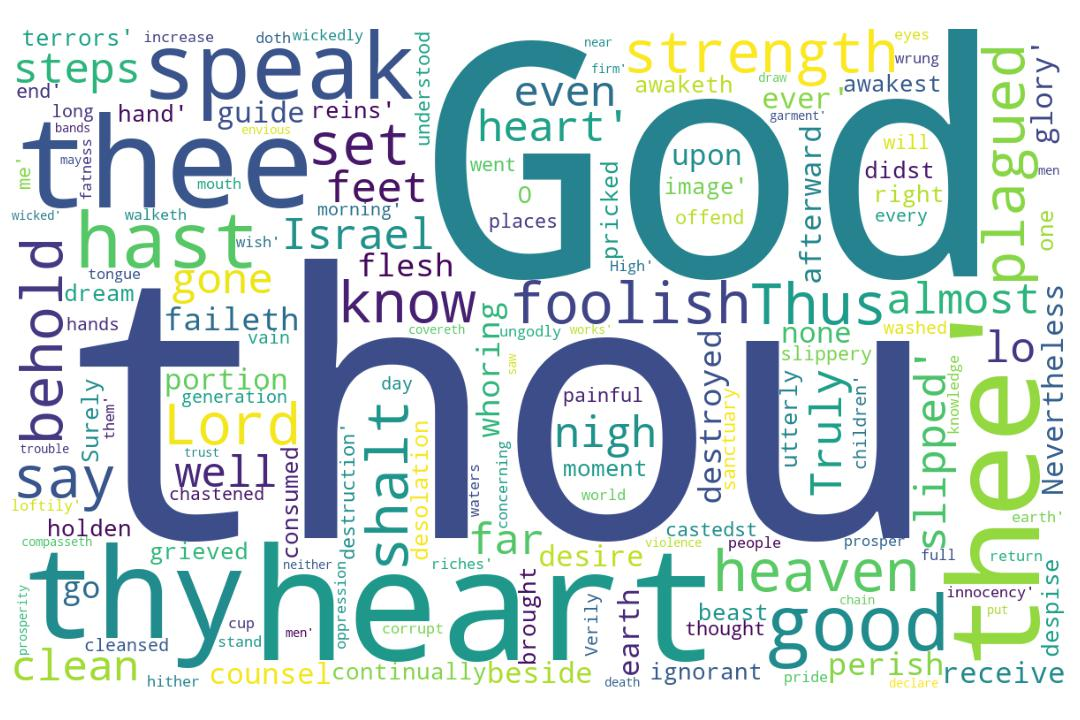
\includegraphics[width=\linewidth]{19OT-Psalms/Psalm73-WordCloud.jpg}
  \caption{Psalm 73 Word Cloud}
  \label{fig:Psalm 73 word Cloud}
\end{figure}

\marginpar{\scriptsize \centering \fcolorbox{bone}{lime}{\textbf{A GOOD GOD}}\\ (Psalm 73:1-28) \begin{compactenum}[I.][8]
    \item \textbf{A Clean Heart} \index[scripture]{Psalms!Psa 073:01}(Psa 73:1)
    \item \textbf{Compassing Hubris} \index[scripture]{Psalms!Psa 073:06}(pride) (Psa 73:6)
    \item \textbf{Corrupt Humanity} \index[scripture]{Psalms!Psa 073:08}(Psa 73:8)
    \item \textbf{Cleansed Hearts} \index[scripture]{Psalms!Psa 073:13}(Psa 73:13)
    \item \textbf{A Cast-Down Heap} \index[scripture]{Psalms!Psa 073:18}(Psa 73:18)
    \item \textbf{A Consuming Horror} \index[scripture]{Psalms!Psa 073:19}(Psa 73:19)
    \item \textbf{A Continual Help} \index[scripture]{Psalms!Psa 073:23}(Psa 73:23)
\end{compactenum}}
    
\marginpar{
\scriptsize \centering 
\fcolorbox{bone}{yellow}{\textbf{THE WICKED \& THEIR PROSPERITY}}\\ (Psalm 73:1-28) \begin{compactenum}[I.][8]
    \item Their \textbf{Compassing} \index[scripture]{Psalms!Psa 073:06}(Psa 73:6)
    \item Their \textbf{Comfort} \index[scripture]{Psalms!Psa 073:07}(Psa 73:7)
    \item Their \textbf{Corruption} \index[scripture]{Psalms!Psa 073:08}(Psa 73:8)
    \item Their \textbf{Concern} \index[scripture]{Psalms!Psa 073:06}(Psa 73:6)
    \item Their \textbf{Conceit} \index[scripture]{Psalms!Psa 073:11}(Psa 73:11)
    \item Their \textbf{Cup} \index[scripture]{Psalms!Psa 073:10}(Psa 73:10)
    \item Their \textbf{Consumption} \index[scripture]{Psalms!Psa 073:18}(Psa 73:18)
\end{compactenum}}

\marginpar{
\scriptsize \centering 
\fcolorbox{bone}{blue}{\textbf{\textcolor[cmyk]{0,0,0,0}{TWO KINDS OF PEOPLE}}}\\
(Psalm 73:1-28) 
\begin{compactenum}[I.][8]
    \item (The Wicked Have) \textbf{Compassing Pride} \index[scripture]{Psalms!Psa 073:06}(Psa 73:6)
    \item (The Wicked Have) \textbf{Covering Violence} \index[scripture]{Psalms!Psa 073:06}(Psa 73:6)
    \item (The Wicked Have) \textbf{Corrupt Speech} \index[scripture]{Psalms!Psa 073:08}(Psa 73:8)
    \item (The Wicked Have) \textbf{A Clear End} \index[scripture]{Psalms!Psa 073:10}(Psa 73:10)
    \item (The Wicked Will Be) \textbf{Cast Down} \index[scripture]{Psalms!Psa 073:18}(Psa 73:18)
    \item (The Wicked Will Be) \textbf{Consumed with Terrors} \index[scripture]{Psalms!Psa 073:19}(Psa 73:19)
    \item (God's People Have) \textbf{Clean Hearts} \index[scripture]{Psalms!Psa 073:01}(Psa 73:1)
    \item (God's People Have God's) \textbf{Continual Presence} \index[scripture]{Psalms!Psa 073:23}(Psa 73:23)
\end{compactenum} }



\footnote{\textcolor[cmyk]{0.99998,1,0,0}{\hyperlink{TOC}{Return to end of Table of Contents.}}}\footnote{\href{https://audiobible.com/bible/psalms_73.html}{\textcolor[cmyk]{0.99998,1,0,0}{Psalm 73 Audio}}}\textcolor[cmyk]{0.99998,1,0,0}{A Psalm of Asaph}\\
\\
\textcolor[cmyk]{0.99998,1,0,0}{Truly God \emph{is} good to Israel, \emph{even} to such as are of a \fcolorbox{bone}{lime}{clean heart}.}
[2] \textcolor[cmyk]{0.99998,1,0,0}{But as for me, my feet were almost gone; my steps had well nigh slipped.}
[3] \textcolor[cmyk]{0.99998,1,0,0}{For I was envious at \fcolorbox{bone}{bone}{the} foolish, \emph{when} I saw \fcolorbox{bone}{bone}{the} prosperity of \fcolorbox{bone}{bone}{the} wicked.}
[4] \textcolor[cmyk]{0.99998,1,0,0}{For \emph{there} \emph{are} no bands in their death: but their strength \emph{is} firm.}
[5] \textcolor[cmyk]{0.99998,1,0,0}{They \emph{are} not in trouble \emph{as} \emph{other} men; neither are they plagued like \emph{other} men.}
[6] \textcolor[cmyk]{0.99998,1,0,0}{Therefore pride \fcolorbox{bone}{lime}{compasseth} them about as a chain; violence covereth them \emph{as} a garment.}
[7] \textcolor[cmyk]{0.99998,1,0,0}{Their eyes stand out with fatness: they have more than heart could wish.}
[8] \textcolor[cmyk]{0.99998,1,0,0}{They are \fcolorbox{bone}{lime}{corrupt}, and speak wickedly \emph{concerning} oppression: they speak loftily.}
[9] \textcolor[cmyk]{0.99998,1,0,0}{They set their mouth against \fcolorbox{bone}{bone}{the} heavens, and their tongue walketh through \fcolorbox{bone}{bone}{the} earth.}
[10] \textcolor[cmyk]{0.99998,1,0,0}{Therefore his people return hither: and waters of a full \emph{cup} are wrung out to them.}
[11] \textcolor[cmyk]{0.99998,1,0,0}{And they say, How doth God know? and is there knowledge in \fcolorbox{bone}{bone}{the} most High?}
[12] \textcolor[cmyk]{0.99998,1,0,0}{Behold, these \emph{are} \fcolorbox{bone}{bone}{the} ungodly, who prosper in \fcolorbox{bone}{bone}{the} world; they increase \emph{in} riches.}
[13] \textcolor[cmyk]{0.99998,1,0,0}{Verily I have \fcolorbox{bone}{lime}{cleansed} my heart \emph{in} vain, and washed my hands in innocency.}
[14] \textcolor[cmyk]{0.99998,1,0,0}{For all \fcolorbox{bone}{bone}{the} day long have I been plagued, and chastened every morning.}
[15] \textcolor[cmyk]{0.99998,1,0,0}{If I say, I will speak thus; behold, I should offend \emph{against} \fcolorbox{bone}{bone}{the} generation of thy children.}
[16] \textcolor[cmyk]{0.99998,1,0,0}{When I thought to know this, it \emph{was} too painful for me;}
[17] \textcolor[cmyk]{0.99998,1,0,0}{Until I went into \fcolorbox{bone}{bone}{the} sanctuary of God; \emph{then} understood I their end.}
[18] \textcolor[cmyk]{0.99998,1,0,0}{Surely thou didst set them in slippery places: thou \fcolorbox{bone}{lime}{castedst} them down into destruction.}
[19] \textcolor[cmyk]{0.99998,1,0,0}{How are they \emph{brought} into desolation, as in a moment! they are utterly \fcolorbox{bone}{lime}{consumed} with terrors.}
[20] \textcolor[cmyk]{0.99998,1,0,0}{As a dream when \emph{one} awaketh; \emph{so}, O Lord, when thou awakest, thou shalt despise their image.}
[21] \textcolor[cmyk]{0.99998,1,0,0}{Thus my heart was grieved, and I was pricked in my reins.}
[22] \textcolor[cmyk]{0.99998,1,0,0}{So foolish \emph{was} I, and ignorant: I was \emph{as} a beast before thee.}
[23] \textcolor[cmyk]{0.99998,1,0,0}{Nevertheless I \emph{am} \fcolorbox{bone}{lime}{continually} with thee: thou hast holden \emph{me} by my right hand.}
[24] \textcolor[cmyk]{0.99998,1,0,0}{Thou shalt guide me with thy counsel, and afterward receive me \emph{to} glory.}
[25] \textcolor[cmyk]{0.99998,1,0,0}{Whom have I in heaven \emph{but} \emph{thee}? and \emph{there} \emph{is} none upon earth \emph{that} I desire beside thee.}
[26] \textcolor[cmyk]{0.99998,1,0,0}{My flesh and my heart faileth: \emph{but} God \emph{is} \fcolorbox{bone}{bone}{the} strength of my heart, and my portion for ever.}
[27] \textcolor[cmyk]{0.99998,1,0,0}{For, lo, they that are far from thee shall perish: thou hast destroyed all them that go a whoring from thee.}
[28] \textcolor[cmyk]{0.99998,1,0,0}{But \emph{it} \emph{is} good for me to draw near to God: I have put my trust in \fcolorbox{bone}{bone}{the} Lord GOD, that I may declare all thy works.}
\index[NWIV]{15!Psalms!Psa 73:1}\index[AWIP]{Truly!Psalms!Psa 73:1}\index[AWIP]{God!Psalms!Psa 73:1}\index[AWIP]{\emph{is}!Psalms!Psa 73:1}\index[AWIP]{good!Psalms!Psa 73:1}\index[AWIP]{to!Psalms!Psa 73:1}\index[AWIP]{to!Psalms!Psa 73:1 (2)}\index[AWIP]{Israel!Psalms!Psa 73:1}\index[AWIP]{\emph{even}!Psalms!Psa 73:1}\index[AWIP]{such!Psalms!Psa 73:1}\index[AWIP]{as!Psalms!Psa 73:1}\index[AWIP]{are!Psalms!Psa 73:1}\index[AWIP]{of!Psalms!Psa 73:1}\index[AWIP]{a!Psalms!Psa 73:1}\index[AWIP]{clean!Psalms!Psa 73:1}\index[AWIP]{heart!Psalms!Psa 73:1}\index[AWIP]{\emph{is}!Psalms!Psa 73:1}\index[AWIP]{\emph{even}!Psalms!Psa 73:1}

\index[NWIV]{15!Psalms!Psa 73:2}\index[AWIP]{But!Psalms!Psa 73:2}\index[AWIP]{as!Psalms!Psa 73:2}\index[AWIP]{for!Psalms!Psa 73:2}\index[AWIP]{me!Psalms!Psa 73:2}\index[AWIP]{my!Psalms!Psa 73:2}\index[AWIP]{my!Psalms!Psa 73:2 (2)}\index[AWIP]{feet!Psalms!Psa 73:2}\index[AWIP]{were!Psalms!Psa 73:2}\index[AWIP]{almost!Psalms!Psa 73:2}\index[AWIP]{gone!Psalms!Psa 73:2}\index[AWIP]{steps!Psalms!Psa 73:2}\index[AWIP]{had!Psalms!Psa 73:2}\index[AWIP]{well!Psalms!Psa 73:2}\index[AWIP]{nigh!Psalms!Psa 73:2}\index[AWIP]{slipped!Psalms!Psa 73:2}

\index[NWIV]{15!Psalms!Psa 73:3}\index[AWIP]{For!Psalms!Psa 73:3}\index[AWIP]{I!Psalms!Psa 73:3}\index[AWIP]{I!Psalms!Psa 73:3 (2)}\index[AWIP]{was!Psalms!Psa 73:3}\index[AWIP]{envious!Psalms!Psa 73:3}\index[AWIP]{at!Psalms!Psa 73:3}\index[AWIP]{the!Psalms!Psa 73:3}\index[AWIP]{the!Psalms!Psa 73:3 (2)}\index[AWIP]{the!Psalms!Psa 73:3 (3)}\index[AWIP]{foolish!Psalms!Psa 73:3}\index[AWIP]{\emph{when}!Psalms!Psa 73:3}\index[AWIP]{saw!Psalms!Psa 73:3}\index[AWIP]{prosperity!Psalms!Psa 73:3}\index[AWIP]{of!Psalms!Psa 73:3}\index[AWIP]{wicked!Psalms!Psa 73:3}\index[AWIP]{\emph{when}!Psalms!Psa 73:3}

\index[NWIV]{13!Psalms!Psa 73:4}\index[AWIP]{For!Psalms!Psa 73:4}\index[AWIP]{\emph{there}!Psalms!Psa 73:4}\index[AWIP]{\emph{are}!Psalms!Psa 73:4}\index[AWIP]{no!Psalms!Psa 73:4}\index[AWIP]{bands!Psalms!Psa 73:4}\index[AWIP]{in!Psalms!Psa 73:4}\index[AWIP]{their!Psalms!Psa 73:4}\index[AWIP]{their!Psalms!Psa 73:4 (2)}\index[AWIP]{death!Psalms!Psa 73:4}\index[AWIP]{but!Psalms!Psa 73:4}\index[AWIP]{strength!Psalms!Psa 73:4}\index[AWIP]{\emph{is}!Psalms!Psa 73:4}\index[AWIP]{firm!Psalms!Psa 73:4}\index[AWIP]{\emph{there}!Psalms!Psa 73:4}\index[AWIP]{\emph{are}!Psalms!Psa 73:4}\index[AWIP]{\emph{is}!Psalms!Psa 73:4}

\index[NWIV]{15!Psalms!Psa 73:5}\index[AWIP]{They!Psalms!Psa 73:5}\index[AWIP]{\emph{are}!Psalms!Psa 73:5}\index[AWIP]{not!Psalms!Psa 73:5}\index[AWIP]{in!Psalms!Psa 73:5}\index[AWIP]{trouble!Psalms!Psa 73:5}\index[AWIP]{\emph{as}!Psalms!Psa 73:5}\index[AWIP]{\emph{other}!Psalms!Psa 73:5}\index[AWIP]{\emph{other}!Psalms!Psa 73:5 (2)}\index[AWIP]{men!Psalms!Psa 73:5}\index[AWIP]{men!Psalms!Psa 73:5 (2)}\index[AWIP]{neither!Psalms!Psa 73:5}\index[AWIP]{are!Psalms!Psa 73:5}\index[AWIP]{they!Psalms!Psa 73:5}\index[AWIP]{plagued!Psalms!Psa 73:5}\index[AWIP]{like!Psalms!Psa 73:5}\index[AWIP]{\emph{are}!Psalms!Psa 73:5}\index[AWIP]{\emph{as}!Psalms!Psa 73:5}\index[AWIP]{\emph{other}!Psalms!Psa 73:5}\index[AWIP]{\emph{other}!Psalms!Psa 73:5 (2)}

\index[NWIV]{14!Psalms!Psa 73:6}\index[AWIP]{Therefore!Psalms!Psa 73:6}\index[AWIP]{pride!Psalms!Psa 73:6}\index[AWIP]{compasseth!Psalms!Psa 73:6}\index[AWIP]{them!Psalms!Psa 73:6}\index[AWIP]{them!Psalms!Psa 73:6 (2)}\index[AWIP]{about!Psalms!Psa 73:6}\index[AWIP]{as!Psalms!Psa 73:6}\index[AWIP]{a!Psalms!Psa 73:6}\index[AWIP]{a!Psalms!Psa 73:6 (2)}\index[AWIP]{chain!Psalms!Psa 73:6}\index[AWIP]{violence!Psalms!Psa 73:6}\index[AWIP]{covereth!Psalms!Psa 73:6}\index[AWIP]{\emph{as}!Psalms!Psa 73:6}\index[AWIP]{garment!Psalms!Psa 73:6}\index[AWIP]{\emph{as}!Psalms!Psa 73:6}

\index[NWIV]{13!Psalms!Psa 73:7}\index[AWIP]{Their!Psalms!Psa 73:7}\index[AWIP]{eyes!Psalms!Psa 73:7}\index[AWIP]{stand!Psalms!Psa 73:7}\index[AWIP]{out!Psalms!Psa 73:7}\index[AWIP]{with!Psalms!Psa 73:7}\index[AWIP]{fatness!Psalms!Psa 73:7}\index[AWIP]{they!Psalms!Psa 73:7}\index[AWIP]{have!Psalms!Psa 73:7}\index[AWIP]{more!Psalms!Psa 73:7}\index[AWIP]{than!Psalms!Psa 73:7}\index[AWIP]{heart!Psalms!Psa 73:7}\index[AWIP]{could!Psalms!Psa 73:7}\index[AWIP]{wish!Psalms!Psa 73:7}

\index[NWIV]{11!Psalms!Psa 73:8}\index[AWIP]{They!Psalms!Psa 73:8}\index[AWIP]{are!Psalms!Psa 73:8}\index[AWIP]{corrupt!Psalms!Psa 73:8}\index[AWIP]{and!Psalms!Psa 73:8}\index[AWIP]{speak!Psalms!Psa 73:8}\index[AWIP]{speak!Psalms!Psa 73:8 (2)}\index[AWIP]{wickedly!Psalms!Psa 73:8}\index[AWIP]{\emph{concerning}!Psalms!Psa 73:8}\index[AWIP]{oppression!Psalms!Psa 73:8}\index[AWIP]{they!Psalms!Psa 73:8}\index[AWIP]{loftily!Psalms!Psa 73:8}\index[AWIP]{\emph{concerning}!Psalms!Psa 73:8}

\index[NWIV]{14!Psalms!Psa 73:9}\index[AWIP]{They!Psalms!Psa 73:9}\index[AWIP]{set!Psalms!Psa 73:9}\index[AWIP]{their!Psalms!Psa 73:9}\index[AWIP]{their!Psalms!Psa 73:9 (2)}\index[AWIP]{mouth!Psalms!Psa 73:9}\index[AWIP]{against!Psalms!Psa 73:9}\index[AWIP]{the!Psalms!Psa 73:9}\index[AWIP]{the!Psalms!Psa 73:9 (2)}\index[AWIP]{heavens!Psalms!Psa 73:9}\index[AWIP]{and!Psalms!Psa 73:9}\index[AWIP]{tongue!Psalms!Psa 73:9}\index[AWIP]{walketh!Psalms!Psa 73:9}\index[AWIP]{through!Psalms!Psa 73:9}\index[AWIP]{earth!Psalms!Psa 73:9}

\index[NWIV]{16!Psalms!Psa 73:10}\index[AWIP]{Therefore!Psalms!Psa 73:10}\index[AWIP]{his!Psalms!Psa 73:10}\index[AWIP]{people!Psalms!Psa 73:10}\index[AWIP]{return!Psalms!Psa 73:10}\index[AWIP]{hither!Psalms!Psa 73:10}\index[AWIP]{and!Psalms!Psa 73:10}\index[AWIP]{waters!Psalms!Psa 73:10}\index[AWIP]{of!Psalms!Psa 73:10}\index[AWIP]{a!Psalms!Psa 73:10}\index[AWIP]{full!Psalms!Psa 73:10}\index[AWIP]{\emph{cup}!Psalms!Psa 73:10}\index[AWIP]{are!Psalms!Psa 73:10}\index[AWIP]{wrung!Psalms!Psa 73:10}\index[AWIP]{out!Psalms!Psa 73:10}\index[AWIP]{to!Psalms!Psa 73:10}\index[AWIP]{them!Psalms!Psa 73:10}\index[AWIP]{\emph{cup}!Psalms!Psa 73:10}

\index[NWIV]{15!Psalms!Psa 73:11}\index[AWIP]{And!Psalms!Psa 73:11}\index[AWIP]{they!Psalms!Psa 73:11}\index[AWIP]{say!Psalms!Psa 73:11}\index[AWIP]{How!Psalms!Psa 73:11}\index[AWIP]{doth!Psalms!Psa 73:11}\index[AWIP]{God!Psalms!Psa 73:11}\index[AWIP]{know?!Psalms!Psa 73:11}\index[AWIP]{and!Psalms!Psa 73:11}\index[AWIP]{is!Psalms!Psa 73:11}\index[AWIP]{there!Psalms!Psa 73:11}\index[AWIP]{knowledge!Psalms!Psa 73:11}\index[AWIP]{in!Psalms!Psa 73:11}\index[AWIP]{the!Psalms!Psa 73:11}\index[AWIP]{most!Psalms!Psa 73:11}\index[AWIP]{High?!Psalms!Psa 73:11}

\index[NWIV]{14!Psalms!Psa 73:12}\index[AWIP]{Behold!Psalms!Psa 73:12}\index[AWIP]{these!Psalms!Psa 73:12}\index[AWIP]{\emph{are}!Psalms!Psa 73:12}\index[AWIP]{the!Psalms!Psa 73:12}\index[AWIP]{the!Psalms!Psa 73:12 (2)}\index[AWIP]{ungodly!Psalms!Psa 73:12}\index[AWIP]{who!Psalms!Psa 73:12}\index[AWIP]{prosper!Psalms!Psa 73:12}\index[AWIP]{in!Psalms!Psa 73:12}\index[AWIP]{world!Psalms!Psa 73:12}\index[AWIP]{they!Psalms!Psa 73:12}\index[AWIP]{increase!Psalms!Psa 73:12}\index[AWIP]{\emph{in}!Psalms!Psa 73:12}\index[AWIP]{riches!Psalms!Psa 73:12}\index[AWIP]{\emph{are}!Psalms!Psa 73:12}\index[AWIP]{\emph{in}!Psalms!Psa 73:12}

\index[NWIV]{14!Psalms!Psa 73:13}\index[AWIP]{Verily!Psalms!Psa 73:13}\index[AWIP]{I!Psalms!Psa 73:13}\index[AWIP]{have!Psalms!Psa 73:13}\index[AWIP]{cleansed!Psalms!Psa 73:13}\index[AWIP]{my!Psalms!Psa 73:13}\index[AWIP]{my!Psalms!Psa 73:13 (2)}\index[AWIP]{heart!Psalms!Psa 73:13}\index[AWIP]{\emph{in}!Psalms!Psa 73:13}\index[AWIP]{vain!Psalms!Psa 73:13}\index[AWIP]{and!Psalms!Psa 73:13}\index[AWIP]{washed!Psalms!Psa 73:13}\index[AWIP]{hands!Psalms!Psa 73:13}\index[AWIP]{in!Psalms!Psa 73:13}\index[AWIP]{innocency!Psalms!Psa 73:13}\index[AWIP]{\emph{in}!Psalms!Psa 73:13}

\index[NWIV]{13!Psalms!Psa 73:14}\index[AWIP]{For!Psalms!Psa 73:14}\index[AWIP]{all!Psalms!Psa 73:14}\index[AWIP]{the!Psalms!Psa 73:14}\index[AWIP]{day!Psalms!Psa 73:14}\index[AWIP]{long!Psalms!Psa 73:14}\index[AWIP]{have!Psalms!Psa 73:14}\index[AWIP]{I!Psalms!Psa 73:14}\index[AWIP]{been!Psalms!Psa 73:14}\index[AWIP]{plagued!Psalms!Psa 73:14}\index[AWIP]{and!Psalms!Psa 73:14}\index[AWIP]{chastened!Psalms!Psa 73:14}\index[AWIP]{every!Psalms!Psa 73:14}\index[AWIP]{morning!Psalms!Psa 73:14}

\index[NWIV]{17!Psalms!Psa 73:15}\index[AWIP]{If!Psalms!Psa 73:15}\index[AWIP]{I!Psalms!Psa 73:15}\index[AWIP]{I!Psalms!Psa 73:15 (2)}\index[AWIP]{I!Psalms!Psa 73:15 (3)}\index[AWIP]{say!Psalms!Psa 73:15}\index[AWIP]{will!Psalms!Psa 73:15}\index[AWIP]{speak!Psalms!Psa 73:15}\index[AWIP]{thus!Psalms!Psa 73:15}\index[AWIP]{behold!Psalms!Psa 73:15}\index[AWIP]{should!Psalms!Psa 73:15}\index[AWIP]{offend!Psalms!Psa 73:15}\index[AWIP]{\emph{against}!Psalms!Psa 73:15}\index[AWIP]{the!Psalms!Psa 73:15}\index[AWIP]{generation!Psalms!Psa 73:15}\index[AWIP]{of!Psalms!Psa 73:15}\index[AWIP]{thy!Psalms!Psa 73:15}\index[AWIP]{children!Psalms!Psa 73:15}\index[AWIP]{\emph{against}!Psalms!Psa 73:15}

\index[NWIV]{12!Psalms!Psa 73:16}\index[AWIP]{When!Psalms!Psa 73:16}\index[AWIP]{I!Psalms!Psa 73:16}\index[AWIP]{thought!Psalms!Psa 73:16}\index[AWIP]{to!Psalms!Psa 73:16}\index[AWIP]{know!Psalms!Psa 73:16}\index[AWIP]{this!Psalms!Psa 73:16}\index[AWIP]{it!Psalms!Psa 73:16}\index[AWIP]{\emph{was}!Psalms!Psa 73:16}\index[AWIP]{too!Psalms!Psa 73:16}\index[AWIP]{painful!Psalms!Psa 73:16}\index[AWIP]{for!Psalms!Psa 73:16}\index[AWIP]{me!Psalms!Psa 73:16}\index[AWIP]{\emph{was}!Psalms!Psa 73:16}

\index[NWIV]{13!Psalms!Psa 73:17}\index[AWIP]{Until!Psalms!Psa 73:17}\index[AWIP]{I!Psalms!Psa 73:17}\index[AWIP]{I!Psalms!Psa 73:17 (2)}\index[AWIP]{went!Psalms!Psa 73:17}\index[AWIP]{into!Psalms!Psa 73:17}\index[AWIP]{the!Psalms!Psa 73:17}\index[AWIP]{sanctuary!Psalms!Psa 73:17}\index[AWIP]{of!Psalms!Psa 73:17}\index[AWIP]{God!Psalms!Psa 73:17}\index[AWIP]{\emph{then}!Psalms!Psa 73:17}\index[AWIP]{understood!Psalms!Psa 73:17}\index[AWIP]{their!Psalms!Psa 73:17}\index[AWIP]{end!Psalms!Psa 73:17}\index[AWIP]{\emph{then}!Psalms!Psa 73:17}

\index[NWIV]{14!Psalms!Psa 73:18}\index[AWIP]{Surely!Psalms!Psa 73:18}\index[AWIP]{thou!Psalms!Psa 73:18}\index[AWIP]{thou!Psalms!Psa 73:18 (2)}\index[AWIP]{didst!Psalms!Psa 73:18}\index[AWIP]{set!Psalms!Psa 73:18}\index[AWIP]{them!Psalms!Psa 73:18}\index[AWIP]{them!Psalms!Psa 73:18 (2)}\index[AWIP]{in!Psalms!Psa 73:18}\index[AWIP]{slippery!Psalms!Psa 73:18}\index[AWIP]{places!Psalms!Psa 73:18}\index[AWIP]{castedst!Psalms!Psa 73:18}\index[AWIP]{down!Psalms!Psa 73:18}\index[AWIP]{into!Psalms!Psa 73:18}\index[AWIP]{destruction!Psalms!Psa 73:18}

\index[NWIV]{16!Psalms!Psa 73:19}\index[AWIP]{How!Psalms!Psa 73:19}\index[AWIP]{are!Psalms!Psa 73:19}\index[AWIP]{are!Psalms!Psa 73:19 (2)}\index[AWIP]{they!Psalms!Psa 73:19}\index[AWIP]{they!Psalms!Psa 73:19 (2)}\index[AWIP]{\emph{brought}!Psalms!Psa 73:19}\index[AWIP]{into!Psalms!Psa 73:19}\index[AWIP]{desolation!Psalms!Psa 73:19}\index[AWIP]{as!Psalms!Psa 73:19}\index[AWIP]{in!Psalms!Psa 73:19}\index[AWIP]{a!Psalms!Psa 73:19}\index[AWIP]{moment!!Psalms!Psa 73:19}\index[AWIP]{utterly!Psalms!Psa 73:19}\index[AWIP]{consumed!Psalms!Psa 73:19}\index[AWIP]{with!Psalms!Psa 73:19}\index[AWIP]{terrors!Psalms!Psa 73:19}\index[AWIP]{\emph{brought}!Psalms!Psa 73:19}

\index[NWIV]{17!Psalms!Psa 73:20}\index[AWIP]{As!Psalms!Psa 73:20}\index[AWIP]{a!Psalms!Psa 73:20}\index[AWIP]{dream!Psalms!Psa 73:20}\index[AWIP]{when!Psalms!Psa 73:20}\index[AWIP]{when!Psalms!Psa 73:20 (2)}\index[AWIP]{\emph{one}!Psalms!Psa 73:20}\index[AWIP]{awaketh!Psalms!Psa 73:20}\index[AWIP]{\emph{so}!Psalms!Psa 73:20}\index[AWIP]{O!Psalms!Psa 73:20}\index[AWIP]{Lord!Psalms!Psa 73:20}\index[AWIP]{thou!Psalms!Psa 73:20}\index[AWIP]{thou!Psalms!Psa 73:20 (2)}\index[AWIP]{awakest!Psalms!Psa 73:20}\index[AWIP]{shalt!Psalms!Psa 73:20}\index[AWIP]{despise!Psalms!Psa 73:20}\index[AWIP]{their!Psalms!Psa 73:20}\index[AWIP]{image!Psalms!Psa 73:20}\index[AWIP]{\emph{one}!Psalms!Psa 73:20}\index[AWIP]{\emph{so}!Psalms!Psa 73:20}

\index[NWIV]{12!Psalms!Psa 73:21}\index[AWIP]{Thus!Psalms!Psa 73:21}\index[AWIP]{my!Psalms!Psa 73:21}\index[AWIP]{my!Psalms!Psa 73:21 (2)}\index[AWIP]{heart!Psalms!Psa 73:21}\index[AWIP]{was!Psalms!Psa 73:21}\index[AWIP]{was!Psalms!Psa 73:21 (2)}\index[AWIP]{grieved!Psalms!Psa 73:21}\index[AWIP]{and!Psalms!Psa 73:21}\index[AWIP]{I!Psalms!Psa 73:21}\index[AWIP]{pricked!Psalms!Psa 73:21}\index[AWIP]{in!Psalms!Psa 73:21}\index[AWIP]{reins!Psalms!Psa 73:21}

\index[NWIV]{13!Psalms!Psa 73:22}\index[AWIP]{So!Psalms!Psa 73:22}\index[AWIP]{foolish!Psalms!Psa 73:22}\index[AWIP]{\emph{was}!Psalms!Psa 73:22}\index[AWIP]{I!Psalms!Psa 73:22}\index[AWIP]{I!Psalms!Psa 73:22 (2)}\index[AWIP]{and!Psalms!Psa 73:22}\index[AWIP]{ignorant!Psalms!Psa 73:22}\index[AWIP]{was!Psalms!Psa 73:22}\index[AWIP]{\emph{as}!Psalms!Psa 73:22}\index[AWIP]{a!Psalms!Psa 73:22}\index[AWIP]{beast!Psalms!Psa 73:22}\index[AWIP]{before!Psalms!Psa 73:22}\index[AWIP]{thee!Psalms!Psa 73:22}\index[AWIP]{\emph{was}!Psalms!Psa 73:22}\index[AWIP]{\emph{as}!Psalms!Psa 73:22}

\index[NWIV]{14!Psalms!Psa 73:23}\index[AWIP]{Nevertheless!Psalms!Psa 73:23}\index[AWIP]{I!Psalms!Psa 73:23}\index[AWIP]{\emph{am}!Psalms!Psa 73:23}\index[AWIP]{continually!Psalms!Psa 73:23}\index[AWIP]{with!Psalms!Psa 73:23}\index[AWIP]{thee!Psalms!Psa 73:23}\index[AWIP]{thou!Psalms!Psa 73:23}\index[AWIP]{hast!Psalms!Psa 73:23}\index[AWIP]{holden!Psalms!Psa 73:23}\index[AWIP]{\emph{me}!Psalms!Psa 73:23}\index[AWIP]{by!Psalms!Psa 73:23}\index[AWIP]{my!Psalms!Psa 73:23}\index[AWIP]{right!Psalms!Psa 73:23}\index[AWIP]{hand!Psalms!Psa 73:23}\index[AWIP]{\emph{am}!Psalms!Psa 73:23}\index[AWIP]{\emph{me}!Psalms!Psa 73:23}

\index[NWIV]{13!Psalms!Psa 73:24}\index[AWIP]{Thou!Psalms!Psa 73:24}\index[AWIP]{shalt!Psalms!Psa 73:24}\index[AWIP]{guide!Psalms!Psa 73:24}\index[AWIP]{me!Psalms!Psa 73:24}\index[AWIP]{me!Psalms!Psa 73:24 (2)}\index[AWIP]{with!Psalms!Psa 73:24}\index[AWIP]{thy!Psalms!Psa 73:24}\index[AWIP]{counsel!Psalms!Psa 73:24}\index[AWIP]{and!Psalms!Psa 73:24}\index[AWIP]{afterward!Psalms!Psa 73:24}\index[AWIP]{receive!Psalms!Psa 73:24}\index[AWIP]{\emph{to}!Psalms!Psa 73:24}\index[AWIP]{glory!Psalms!Psa 73:24}\index[AWIP]{\emph{to}!Psalms!Psa 73:24}

\index[NWIV]{18!Psalms!Psa 73:25}\index[AWIP]{Whom!Psalms!Psa 73:25}\index[AWIP]{have!Psalms!Psa 73:25}\index[AWIP]{I!Psalms!Psa 73:25}\index[AWIP]{I!Psalms!Psa 73:25 (2)}\index[AWIP]{in!Psalms!Psa 73:25}\index[AWIP]{heaven!Psalms!Psa 73:25}\index[AWIP]{\emph{but}!Psalms!Psa 73:25}\index[AWIP]{\emph{thee}?!Psalms!Psa 73:25}\index[AWIP]{and!Psalms!Psa 73:25}\index[AWIP]{\emph{there}!Psalms!Psa 73:25}\index[AWIP]{\emph{is}!Psalms!Psa 73:25}\index[AWIP]{none!Psalms!Psa 73:25}\index[AWIP]{upon!Psalms!Psa 73:25}\index[AWIP]{earth!Psalms!Psa 73:25}\index[AWIP]{\emph{that}!Psalms!Psa 73:25}\index[AWIP]{desire!Psalms!Psa 73:25}\index[AWIP]{beside!Psalms!Psa 73:25}\index[AWIP]{thee!Psalms!Psa 73:25}\index[AWIP]{\emph{but}!Psalms!Psa 73:25}\index[AWIP]{\emph{thee}?!Psalms!Psa 73:25}\index[AWIP]{\emph{there}!Psalms!Psa 73:25}\index[AWIP]{\emph{is}!Psalms!Psa 73:25}\index[AWIP]{\emph{that}!Psalms!Psa 73:25}

\index[NWIV]{19!Psalms!Psa 73:26}\index[AWIP]{My!Psalms!Psa 73:26}\index[AWIP]{flesh!Psalms!Psa 73:26}\index[AWIP]{and!Psalms!Psa 73:26}\index[AWIP]{and!Psalms!Psa 73:26 (2)}\index[AWIP]{my!Psalms!Psa 73:26}\index[AWIP]{my!Psalms!Psa 73:26 (2)}\index[AWIP]{my!Psalms!Psa 73:26 (3)}\index[AWIP]{heart!Psalms!Psa 73:26}\index[AWIP]{heart!Psalms!Psa 73:26 (2)}\index[AWIP]{faileth!Psalms!Psa 73:26}\index[AWIP]{\emph{but}!Psalms!Psa 73:26}\index[AWIP]{God!Psalms!Psa 73:26}\index[AWIP]{\emph{is}!Psalms!Psa 73:26}\index[AWIP]{the!Psalms!Psa 73:26}\index[AWIP]{strength!Psalms!Psa 73:26}\index[AWIP]{of!Psalms!Psa 73:26}\index[AWIP]{portion!Psalms!Psa 73:26}\index[AWIP]{for!Psalms!Psa 73:26}\index[AWIP]{ever!Psalms!Psa 73:26}\index[AWIP]{\emph{but}!Psalms!Psa 73:26}\index[AWIP]{\emph{is}!Psalms!Psa 73:26}

\index[NWIV]{21!Psalms!Psa 73:27}\index[AWIP]{For!Psalms!Psa 73:27}\index[AWIP]{lo!Psalms!Psa 73:27}\index[AWIP]{they!Psalms!Psa 73:27}\index[AWIP]{that!Psalms!Psa 73:27}\index[AWIP]{that!Psalms!Psa 73:27 (2)}\index[AWIP]{are!Psalms!Psa 73:27}\index[AWIP]{far!Psalms!Psa 73:27}\index[AWIP]{from!Psalms!Psa 73:27}\index[AWIP]{from!Psalms!Psa 73:27 (2)}\index[AWIP]{thee!Psalms!Psa 73:27}\index[AWIP]{thee!Psalms!Psa 73:27 (2)}\index[AWIP]{shall!Psalms!Psa 73:27}\index[AWIP]{perish!Psalms!Psa 73:27}\index[AWIP]{thou!Psalms!Psa 73:27}\index[AWIP]{hast!Psalms!Psa 73:27}\index[AWIP]{destroyed!Psalms!Psa 73:27}\index[AWIP]{all!Psalms!Psa 73:27}\index[AWIP]{them!Psalms!Psa 73:27}\index[AWIP]{go!Psalms!Psa 73:27}\index[AWIP]{a!Psalms!Psa 73:27}\index[AWIP]{whoring!Psalms!Psa 73:27}

\index[NWIV]{27!Psalms!Psa 73:28}\index[AWIP]{But!Psalms!Psa 73:28}\index[AWIP]{\emph{it}!Psalms!Psa 73:28}\index[AWIP]{\emph{is}!Psalms!Psa 73:28}\index[AWIP]{good!Psalms!Psa 73:28}\index[AWIP]{for!Psalms!Psa 73:28}\index[AWIP]{me!Psalms!Psa 73:28}\index[AWIP]{to!Psalms!Psa 73:28}\index[AWIP]{to!Psalms!Psa 73:28 (2)}\index[AWIP]{draw!Psalms!Psa 73:28}\index[AWIP]{near!Psalms!Psa 73:28}\index[AWIP]{God!Psalms!Psa 73:28}\index[AWIP]{I!Psalms!Psa 73:28}\index[AWIP]{I!Psalms!Psa 73:28 (2)}\index[AWIP]{have!Psalms!Psa 73:28}\index[AWIP]{put!Psalms!Psa 73:28}\index[AWIP]{my!Psalms!Psa 73:28}\index[AWIP]{trust!Psalms!Psa 73:28}\index[AWIP]{in!Psalms!Psa 73:28}\index[AWIP]{the!Psalms!Psa 73:28}\index[AWIP]{Lord!Psalms!Psa 73:28}\index[AWIP]{GOD!Psalms!Psa 73:28}\index[AWIP]{that!Psalms!Psa 73:28}\index[AWIP]{may!Psalms!Psa 73:28}\index[AWIP]{declare!Psalms!Psa 73:28}\index[AWIP]{all!Psalms!Psa 73:28}\index[AWIP]{thy!Psalms!Psa 73:28}\index[AWIP]{works!Psalms!Psa 73:28}\index[AWIP]{\emph{it}!Psalms!Psa 73:28}\index[AWIP]{\emph{is}!Psalms!Psa 73:28}


\section{Psalm 73 Outlines}

\subsection{My Outlines} 

\subsubsection{A Good God}
%Psalm 73:\footnote{18 August 2015, Keith Anthony}
\index[speaker]{Keith Anthony!Psalm 073 (A Good God)}
\index[series]{Psalms (Keith Anthony)!Psalm 073 (A Good God)}
\index[date]{2015/08/18!Psalm 073 (A Good God) (Keith Anthony)}

\begin{compactenum}[I.]
    \item \textbf{A Clean Heart} \index[scripture]{Psalms!Psa 073:01}(Psa 73:1)
    \item \textbf{Compassing Hubris} \index[scripture]{Psalms!Psa 073:06}(pride) (Psa 73:6)
    \item \textbf{Corrupt Humanity} \index[scripture]{Psalms!Psa 073:08}(Psa 73:8)
    \item \textbf{Cleansed Hearts} \index[scripture]{Psalms!Psa 073:13}(Psa 73:13)
    \item \textbf{A Cast-Down Heap} \index[scripture]{Psalms!Psa 073:18}(Psa 73:18)
    \item \textbf{A Consuming Horror} \index[scripture]{Psalms!Psa 073:19}(Psa 73:19)
    \item \textbf{A Continual Help} \index[scripture]{Psalms!Psa 073:23}(Psa 73:23)
\end{compactenum}



\subsubsection{The Wicked \& their Prosperity}
%Psalm 73:\footnote{17 August 2016, Keith Anthony}
\index[speaker]{Keith Anthony!Psalm 073 (The Wicked \& their Prosperity)}
\index[series]{Psalms (Keith Anthony)!Psalm 073 (The Wicked \& their Prosperity)}
\index[date]{2020/09/01!Psalm 073 (The Wicked \& their Prosperity) (Keith Anthony)}

 \begin{compactenum}[I.][8]
    \item Their \textbf{Compassing} \index[scripture]{Psalms!Psa 073:06}(Psa 73:6)
    \item Their \textbf{Comfort} \index[scripture]{Psalms!Psa 073:07}(Psa 73:7)
    \item Their \textbf{Corruption} \index[scripture]{Psalms!Psa 073:08}(Psa 73:8)
    \item Their \textbf{Concern} \index[scripture]{Psalms!Psa 073:06}(Psa 73:6)
    \item Their \textbf{Conceit} \index[scripture]{Psalms!Psa 073:11}(Psa 73:11)
    \item Their \textbf{Cup} \index[scripture]{Psalms!Psa 073:10}(Psa 73:10)
    \item Their \textbf{Consumption} \index[scripture]{Psalms!Psa 073:18}(Psa 73:18)
\end{compactenum}


\subsubsection{Two Kinds of People}
%Psalm 73:\footnote{17 August 2016, Keith Anthony}
\index[speaker]{Keith Anthony!Psalm 073 (Two Kinds of People)}
\index[series]{Psalms (Keith Anthony)!Psalm 073 (Two Kinds of People)}
\index[date]{2015/08/18!Psalm 073 (Two Kinds of People) (Keith Anthony)}

\begin{compactenum}[I.]
    \item (The Wicked Have) \textbf{Compassing Pride} \index[scripture]{Psalms!Psa 073:06}(Psa 73:6)
    \item (The Wicked Have) \textbf{Covering Violence} \index[scripture]{Psalms!Psa 073:06}(Psa 73:6)
    \item (The Wicked Have) \textbf{Corrupt Speech} \index[scripture]{Psalms!Psa 073:08}(Psa 73:8)
    \item (The Wicked Have) \textbf{A Clear End} \index[scripture]{Psalms!Psa 073:10}(Psa 73:10)
    \item (The Wicked Will Be) \textbf{Cast Down} \index[scripture]{Psalms!Psa 073:18}(Psa 73:18)
    \item (The Wicked Will Be) \textbf{Consumed with Terrors} \index[scripture]{Psalms!Psa 073:19}(Psa 73:19)
    \item (God's People Have) \textbf{Clean Hearts} \index[scripture]{Psalms!Psa 073:01}(Psa 73:1)
    \item (God's People Have God's) \textbf{Continual Presence} \index[scripture]{Psalms!Psa 073:23}(Psa 73:23)
\end{compactenum}

\subsection{Outlines from Others}


\section{Psalm 73 Comments}

\subsection{Numeric Nuggets}
There are 13 words in verses 4, 7, 14, 17, 22, and 24. There are 13 unique words in verses 5, 7, 12, 13, and 14.  The word ``the'' is used 13 times in the psalm.
\subsection{Psalm 73 Repeated Phrases}


%%%%%%%%%%
%%%%%%%%%%
\normalsize
 
\begin{center}
\begin{longtable}{|p{3.0in}|p{0.5in}|}
\caption[Psal m 73 Repeated Phrases]{Psalm 73 Repeated Phrases}\label{table:Repeated Phrases Psalm73} \\
\hline \multicolumn{1}{|c|}{\textbf{Phrase}} & \multicolumn{1}{c|}{\textbf{Frequency}} \\ \hline 
\endfirsthead
 
\multicolumn{2}{c}
{{\bfseries \tablename\ \thetable{} -- continued from previous page}} \\  
\hline \multicolumn{1}{|c|}{\textbf{Phrase}} & \multicolumn{1}{c|}{\textbf{Frequency}} \\ \hline 
\endhead
 
\hline \multicolumn{2}{c}{{ }} \\ \hline
\endfoot 
my heart & 4\\ \hline 
for me & 3\\ \hline 
I was & 3\\ \hline 
in the & 3\\ \hline 
\end{longtable}
\end{center}



%%%%%%%%%%
%%%%%%%%%%



\section{Psalm 73 Statistics}

%%%%%%%%%%%%%%%%%%%%%%%%%%%
%%%%% Word Statistics
%%%%%%%%%%%%%%%%%%%%%%%%%%


\normalsize



\subsection{Chapter Word Statistics}


%%%%%%%%%%
%%%%%%%%%%
 
\begin{center}
\begin{longtable}{l|c|c|c|c}
\caption[Stats for Psalm 73]{Stats for Psalm 73} \label{table:Stats for Psalm 73} \\ 
\hline \multicolumn{1}{|c|}{\textbf{Verse(s)}} & \multicolumn{1}{|c|}{\textbf{Count}} & \multicolumn{1}{|c|}{\textbf{Unique}} & \multicolumn{1}{|c|}{\textbf{Italics}} & \multicolumn{1}{|c|}{\textbf{Uniq Italic}}  \\ \hline 
\endfirsthead
 
\multicolumn{5}{c}
{{\bfseries \tablename\ \thetable{} -- continued from previous page}} \\  
\hline \multicolumn{1}{|c|}{\textbf{Verse(s)}} & \multicolumn{1}{|c|}{\textbf{Count}} & \multicolumn{1}{|c|}{\textbf{Unique}} & \multicolumn{1}{|c|}{\textbf{Italics}} & \multicolumn{1}{|c|}{\textbf{Uniq Italic}}  \\ \hline 
\endhead
 
\hline \multicolumn{5}{|r|}{{Continued if needed}} \\ \hline
\endfoot 
1 & 15 & 14 & 2 & 2\\ \hline
2 & 15 & 14 & 0 & 0\\ \hline
3 & 15 & 12 & 1 & 1\\ \hline
4 & 13 & 12 & 3 & 3\\ \hline
5 & 15 & 13 & 4 & 3\\ \hline
6 & 14 & 12 & 1 & 1\\ \hline
7 & 13 & 13 & 0 & 0\\ \hline
8 & 11 & 10 & 1 & 1\\ \hline
9 & 14 & 12 & 0 & 0\\ \hline
10 & 16 & 16 & 1 & 1\\ \hline
11 & 15 & 15 & 0 & 0\\ \hline
12 & 14 & 13 & 2 & 2\\ \hline
13 & 14 & 13 & 1 & 1\\ \hline
14 & 13 & 13 & 0 & 0\\ \hline
15 & 17 & 15 & 1 & 1\\ \hline
16 & 12 & 12 & 1 & 1\\ \hline
17 & 13 & 12 & 1 & 1\\ \hline
18 & 14 & 12 & 0 & 0\\ \hline
19 & 16 & 14 & 1 & 1\\ \hline
20 & 17 & 15 & 2 & 2\\ \hline
21 & 12 & 10 & 0 & 0\\ \hline
22 & 13 & 12 & 2 & 2\\ \hline
23 & 14 & 14 & 2 & 2\\ \hline
24 & 13 & 12 & 1 & 1\\ \hline
25 & 18 & 17 & 5 & 5\\ \hline
26 & 19 & 15 & 2 & 2\\ \hline
27 & 21 & 18 & 0 & 0\\ \hline
28 & 27 & 25 & 2 & 2\\ \hline
\hline \hline
Total & 423 & 240 & 36 & 23



\end{longtable}
\end{center}

%%%%%%%%%%
%%%%%%%%%%
 
\subsection{Words by Frequency}

\begin{center}
\begin{longtable}{l|r}
\caption[Word Frequencies in Psalm 73]{Word Frequencies in Psalm 73} \label{table:WordsIn-Psalm-73} \\ 
\hline \multicolumn{1}{|c|}{\textbf{Word}} & \multicolumn{1}{c|}{\textbf{Frequency}} \\ \hline 
\endfirsthead
 
\multicolumn{2}{c}
{{\bfseries \tablename\ \thetable{} -- continued from previous page}} \\ 
\hline \multicolumn{1}{|c|}{\textbf{Word}} & \multicolumn{1}{c|}{\textbf{Frequency}} \\ \hline 
\endhead
 
\hline \multicolumn{2}{|r|}{{Continued if needed}} \\ \hline
\endfoot
 
\hline \hline
\endlastfoot
I & 18 \\ \hline
the & 13 \\ \hline
and & 12 \\ \hline
my & 11 \\ \hline
in & 10 \\ \hline
a & 8 \\ \hline
they & 8 \\ \hline
are & 7 \\ \hline
to & 6 \\ \hline
of & 6 \\ \hline
heart & 6 \\ \hline
their & 6 \\ \hline
them & 6 \\ \hline
thou & 6 \\ \hline
God & 5 \\ \hline
\emph{is} & 5 \\ \hline
me & 5 \\ \hline
have & 5 \\ \hline
thee & 5 \\ \hline
as & 4 \\ \hline
for & 4 \\ \hline
For & 4 \\ \hline
was & 4 \\ \hline
with & 4 \\ \hline
\emph{are} & 3 \\ \hline
They & 3 \\ \hline
\emph{as} & 3 \\ \hline
speak & 3 \\ \hline
all & 3 \\ \hline
thy & 3 \\ \hline
into & 3 \\ \hline
that & 3 \\ \hline
good & 2 \\ \hline
But & 2 \\ \hline
foolish & 2 \\ \hline
\emph{there} & 2 \\ \hline
strength & 2 \\ \hline
\emph{other} & 2 \\ \hline
men & 2 \\ \hline
plagued & 2 \\ \hline
Therefore & 2 \\ \hline
out & 2 \\ \hline
set & 2 \\ \hline
earth & 2 \\ \hline
say & 2 \\ \hline
How & 2 \\ \hline
know & 2 \\ \hline
\emph{in} & 2 \\ \hline
\emph{was} & 2 \\ \hline
when & 2 \\ \hline
Lord & 2 \\ \hline
shalt & 2 \\ \hline
hast & 2 \\ \hline
\emph{but} & 2 \\ \hline
from & 2 \\ \hline
Truly & 1 \\ \hline
Israel & 1 \\ \hline
\emph{even} & 1 \\ \hline
such & 1 \\ \hline
clean & 1 \\ \hline
feet & 1 \\ \hline
were & 1 \\ \hline
almost & 1 \\ \hline
gone & 1 \\ \hline
steps & 1 \\ \hline
had & 1 \\ \hline
well & 1 \\ \hline
nigh & 1 \\ \hline
slipped & 1 \\ \hline
envious & 1 \\ \hline
at & 1 \\ \hline
\emph{when} & 1 \\ \hline
saw & 1 \\ \hline
prosperity & 1 \\ \hline
wicked & 1 \\ \hline
no & 1 \\ \hline
bands & 1 \\ \hline
death & 1 \\ \hline
but & 1 \\ \hline
firm & 1 \\ \hline
not & 1 \\ \hline
trouble & 1 \\ \hline
neither & 1 \\ \hline
like & 1 \\ \hline
pride & 1 \\ \hline
compasseth & 1 \\ \hline
about & 1 \\ \hline
chain & 1 \\ \hline
violence & 1 \\ \hline
covereth & 1 \\ \hline
garment & 1 \\ \hline
Their & 1 \\ \hline
eyes & 1 \\ \hline
stand & 1 \\ \hline
fatness & 1 \\ \hline
more & 1 \\ \hline
than & 1 \\ \hline
could & 1 \\ \hline
wish & 1 \\ \hline
corrupt & 1 \\ \hline
wickedly & 1 \\ \hline
\emph{concerning} & 1 \\ \hline
oppression & 1 \\ \hline
loftily & 1 \\ \hline
mouth & 1 \\ \hline
against & 1 \\ \hline
heavens & 1 \\ \hline
tongue & 1 \\ \hline
walketh & 1 \\ \hline
through & 1 \\ \hline
his & 1 \\ \hline
people & 1 \\ \hline
return & 1 \\ \hline
hither & 1 \\ \hline
waters & 1 \\ \hline
full & 1 \\ \hline
\emph{cup} & 1 \\ \hline
wrung & 1 \\ \hline
And & 1 \\ \hline
doth & 1 \\ \hline
is & 1 \\ \hline
there & 1 \\ \hline
knowledge & 1 \\ \hline
most & 1 \\ \hline
High & 1 \\ \hline
Behold & 1 \\ \hline
these & 1 \\ \hline
ungodly & 1 \\ \hline
who & 1 \\ \hline
prosper & 1 \\ \hline
world & 1 \\ \hline
increase & 1 \\ \hline
riches & 1 \\ \hline
Verily & 1 \\ \hline
cleansed & 1 \\ \hline
vain & 1 \\ \hline
washed & 1 \\ \hline
hands & 1 \\ \hline
innocency & 1 \\ \hline
day & 1 \\ \hline
long & 1 \\ \hline
been & 1 \\ \hline
chastened & 1 \\ \hline
every & 1 \\ \hline
morning & 1 \\ \hline
If & 1 \\ \hline
will & 1 \\ \hline
thus & 1 \\ \hline
behold & 1 \\ \hline
should & 1 \\ \hline
offend & 1 \\ \hline
\emph{against} & 1 \\ \hline
generation & 1 \\ \hline
children & 1 \\ \hline
When & 1 \\ \hline
thought & 1 \\ \hline
this & 1 \\ \hline
it & 1 \\ \hline
too & 1 \\ \hline
painful & 1 \\ \hline
Until & 1 \\ \hline
went & 1 \\ \hline
sanctuary & 1 \\ \hline
\emph{then} & 1 \\ \hline
understood & 1 \\ \hline
end & 1 \\ \hline
Surely & 1 \\ \hline
didst & 1 \\ \hline
slippery & 1 \\ \hline
places & 1 \\ \hline
castedst & 1 \\ \hline
down & 1 \\ \hline
destruction & 1 \\ \hline
\emph{brought} & 1 \\ \hline
desolation & 1 \\ \hline
moment & 1 \\ \hline
utterly & 1 \\ \hline
consumed & 1 \\ \hline
terrors & 1 \\ \hline
As & 1 \\ \hline
dream & 1 \\ \hline
\emph{one} & 1 \\ \hline
awaketh & 1 \\ \hline
\emph{so} & 1 \\ \hline
O & 1 \\ \hline
awakest & 1 \\ \hline
despise & 1 \\ \hline
image & 1 \\ \hline
Thus & 1 \\ \hline
grieved & 1 \\ \hline
pricked & 1 \\ \hline
reins & 1 \\ \hline
So & 1 \\ \hline
ignorant & 1 \\ \hline
beast & 1 \\ \hline
before & 1 \\ \hline
Nevertheless & 1 \\ \hline
\emph{am} & 1 \\ \hline
continually & 1 \\ \hline
holden & 1 \\ \hline
\emph{me} & 1 \\ \hline
by & 1 \\ \hline
right & 1 \\ \hline
hand & 1 \\ \hline
Thou & 1 \\ \hline
guide & 1 \\ \hline
counsel & 1 \\ \hline
afterward & 1 \\ \hline
receive & 1 \\ \hline
\emph{to} & 1 \\ \hline
glory & 1 \\ \hline
Whom & 1 \\ \hline
heaven & 1 \\ \hline
\emph{thee} & 1 \\ \hline
none & 1 \\ \hline
upon & 1 \\ \hline
\emph{that} & 1 \\ \hline
desire & 1 \\ \hline
beside & 1 \\ \hline
My & 1 \\ \hline
flesh & 1 \\ \hline
faileth & 1 \\ \hline
portion & 1 \\ \hline
ever & 1 \\ \hline
lo & 1 \\ \hline
far & 1 \\ \hline
shall & 1 \\ \hline
perish & 1 \\ \hline
destroyed & 1 \\ \hline
go & 1 \\ \hline
whoring & 1 \\ \hline
\emph{it} & 1 \\ \hline
draw & 1 \\ \hline
near & 1 \\ \hline
put & 1 \\ \hline
trust & 1 \\ \hline
GOD & 1 \\ \hline
may & 1 \\ \hline
declare & 1 \\ \hline
works & 1 \\ \hline
\end{longtable}
\end{center}



\normalsize



\subsection{Words Alphabetically}

\begin{center}
\begin{longtable}{l|r}
\caption[Word Alphabetically in Psalm 73]{Word Alphabetically in Psalm 73} \label{table:WordsIn-Psalm-73} \\ 
\hline \multicolumn{1}{|c|}{\textbf{Word}} & \multicolumn{1}{c|}{\textbf{Frequency}} \\ \hline 
\endfirsthead
 
\multicolumn{2}{c}
{{\bfseries \tablename\ \thetable{} -- continued from previous page}} \\ 
\hline \multicolumn{1}{|c|}{\textbf{Word}} & \multicolumn{1}{c|}{\textbf{Frequency}} \\ \hline 
\endhead
 
\hline \multicolumn{2}{|r|}{{Continued if needed}} \\ \hline
\endfoot
 
\hline \hline
\endlastfoot
And & 1 \\ \hline
As & 1 \\ \hline
Behold & 1 \\ \hline
But & 2 \\ \hline
For & 4 \\ \hline
GOD & 1 \\ \hline
God & 5 \\ \hline
High & 1 \\ \hline
How & 2 \\ \hline
I & 18 \\ \hline
If & 1 \\ \hline
Israel & 1 \\ \hline
Lord & 2 \\ \hline
My & 1 \\ \hline
Nevertheless & 1 \\ \hline
O & 1 \\ \hline
So & 1 \\ \hline
Surely & 1 \\ \hline
Their & 1 \\ \hline
Therefore & 2 \\ \hline
They & 3 \\ \hline
Thou & 1 \\ \hline
Thus & 1 \\ \hline
Truly & 1 \\ \hline
Until & 1 \\ \hline
Verily & 1 \\ \hline
When & 1 \\ \hline
Whom & 1 \\ \hline
\emph{against} & 1 \\ \hline
\emph{am} & 1 \\ \hline
\emph{are} & 3 \\ \hline
\emph{as} & 3 \\ \hline
\emph{brought} & 1 \\ \hline
\emph{but} & 2 \\ \hline
\emph{concerning} & 1 \\ \hline
\emph{cup} & 1 \\ \hline
\emph{even} & 1 \\ \hline
\emph{in} & 2 \\ \hline
\emph{is} & 5 \\ \hline
\emph{it} & 1 \\ \hline
\emph{me} & 1 \\ \hline
\emph{one} & 1 \\ \hline
\emph{other} & 2 \\ \hline
\emph{so} & 1 \\ \hline
\emph{that} & 1 \\ \hline
\emph{thee} & 1 \\ \hline
\emph{then} & 1 \\ \hline
\emph{there} & 2 \\ \hline
\emph{to} & 1 \\ \hline
\emph{was} & 2 \\ \hline
\emph{when} & 1 \\ \hline
a & 8 \\ \hline
about & 1 \\ \hline
afterward & 1 \\ \hline
against & 1 \\ \hline
all & 3 \\ \hline
almost & 1 \\ \hline
and & 12 \\ \hline
are & 7 \\ \hline
as & 4 \\ \hline
at & 1 \\ \hline
awakest & 1 \\ \hline
awaketh & 1 \\ \hline
bands & 1 \\ \hline
beast & 1 \\ \hline
been & 1 \\ \hline
before & 1 \\ \hline
behold & 1 \\ \hline
beside & 1 \\ \hline
but & 1 \\ \hline
by & 1 \\ \hline
castedst & 1 \\ \hline
chain & 1 \\ \hline
chastened & 1 \\ \hline
children & 1 \\ \hline
clean & 1 \\ \hline
cleansed & 1 \\ \hline
compasseth & 1 \\ \hline
consumed & 1 \\ \hline
continually & 1 \\ \hline
corrupt & 1 \\ \hline
could & 1 \\ \hline
counsel & 1 \\ \hline
covereth & 1 \\ \hline
day & 1 \\ \hline
death & 1 \\ \hline
declare & 1 \\ \hline
desire & 1 \\ \hline
desolation & 1 \\ \hline
despise & 1 \\ \hline
destroyed & 1 \\ \hline
destruction & 1 \\ \hline
didst & 1 \\ \hline
doth & 1 \\ \hline
down & 1 \\ \hline
draw & 1 \\ \hline
dream & 1 \\ \hline
earth & 2 \\ \hline
end & 1 \\ \hline
envious & 1 \\ \hline
ever & 1 \\ \hline
every & 1 \\ \hline
eyes & 1 \\ \hline
faileth & 1 \\ \hline
far & 1 \\ \hline
fatness & 1 \\ \hline
feet & 1 \\ \hline
firm & 1 \\ \hline
flesh & 1 \\ \hline
foolish & 2 \\ \hline
for & 4 \\ \hline
from & 2 \\ \hline
full & 1 \\ \hline
garment & 1 \\ \hline
generation & 1 \\ \hline
glory & 1 \\ \hline
go & 1 \\ \hline
gone & 1 \\ \hline
good & 2 \\ \hline
grieved & 1 \\ \hline
guide & 1 \\ \hline
had & 1 \\ \hline
hand & 1 \\ \hline
hands & 1 \\ \hline
hast & 2 \\ \hline
have & 5 \\ \hline
heart & 6 \\ \hline
heaven & 1 \\ \hline
heavens & 1 \\ \hline
his & 1 \\ \hline
hither & 1 \\ \hline
holden & 1 \\ \hline
ignorant & 1 \\ \hline
image & 1 \\ \hline
in & 10 \\ \hline
increase & 1 \\ \hline
innocency & 1 \\ \hline
into & 3 \\ \hline
is & 1 \\ \hline
it & 1 \\ \hline
know & 2 \\ \hline
knowledge & 1 \\ \hline
like & 1 \\ \hline
lo & 1 \\ \hline
loftily & 1 \\ \hline
long & 1 \\ \hline
may & 1 \\ \hline
me & 5 \\ \hline
men & 2 \\ \hline
moment & 1 \\ \hline
more & 1 \\ \hline
morning & 1 \\ \hline
most & 1 \\ \hline
mouth & 1 \\ \hline
my & 11 \\ \hline
near & 1 \\ \hline
neither & 1 \\ \hline
nigh & 1 \\ \hline
no & 1 \\ \hline
none & 1 \\ \hline
not & 1 \\ \hline
of & 6 \\ \hline
offend & 1 \\ \hline
oppression & 1 \\ \hline
out & 2 \\ \hline
painful & 1 \\ \hline
people & 1 \\ \hline
perish & 1 \\ \hline
places & 1 \\ \hline
plagued & 2 \\ \hline
portion & 1 \\ \hline
pricked & 1 \\ \hline
pride & 1 \\ \hline
prosper & 1 \\ \hline
prosperity & 1 \\ \hline
put & 1 \\ \hline
receive & 1 \\ \hline
reins & 1 \\ \hline
return & 1 \\ \hline
riches & 1 \\ \hline
right & 1 \\ \hline
sanctuary & 1 \\ \hline
saw & 1 \\ \hline
say & 2 \\ \hline
set & 2 \\ \hline
shall & 1 \\ \hline
shalt & 2 \\ \hline
should & 1 \\ \hline
slipped & 1 \\ \hline
slippery & 1 \\ \hline
speak & 3 \\ \hline
stand & 1 \\ \hline
steps & 1 \\ \hline
strength & 2 \\ \hline
such & 1 \\ \hline
terrors & 1 \\ \hline
than & 1 \\ \hline
that & 3 \\ \hline
the & 13 \\ \hline
thee & 5 \\ \hline
their & 6 \\ \hline
them & 6 \\ \hline
there & 1 \\ \hline
these & 1 \\ \hline
they & 8 \\ \hline
this & 1 \\ \hline
thou & 6 \\ \hline
thought & 1 \\ \hline
through & 1 \\ \hline
thus & 1 \\ \hline
thy & 3 \\ \hline
to & 6 \\ \hline
tongue & 1 \\ \hline
too & 1 \\ \hline
trouble & 1 \\ \hline
trust & 1 \\ \hline
understood & 1 \\ \hline
ungodly & 1 \\ \hline
upon & 1 \\ \hline
utterly & 1 \\ \hline
vain & 1 \\ \hline
violence & 1 \\ \hline
walketh & 1 \\ \hline
was & 4 \\ \hline
washed & 1 \\ \hline
waters & 1 \\ \hline
well & 1 \\ \hline
went & 1 \\ \hline
were & 1 \\ \hline
when & 2 \\ \hline
who & 1 \\ \hline
whoring & 1 \\ \hline
wicked & 1 \\ \hline
wickedly & 1 \\ \hline
will & 1 \\ \hline
wish & 1 \\ \hline
with & 4 \\ \hline
works & 1 \\ \hline
world & 1 \\ \hline
wrung & 1 \\ \hline
\end{longtable}
\end{center}



\normalsize



\subsection{Word Lengths in Chapter}
\normalsize
\begin{longtable}{l|p{3.75in}}
\caption[Words by Length in Psalm 73]{Words by Length in Psalm 73} \label{table:WordsIn-Psalm-73} \\ 
\hline \multicolumn{1}{|c|}{\textbf{Length}} & \multicolumn{1}{c|}{\textbf{Words}} \\ \hline 
\endfirsthead
 
\multicolumn{2}{c}
{{\bfseries \tablename\ \thetable{} -- continued from previous page}} \\ 
\hline \multicolumn{1}{|c|}{\textbf{Length}} & \multicolumn{1}{c|}{\textbf{Words}} \\ \hline 
\endhead
 
\hline \multicolumn{2}{|r|}{{Continued if needed}} \\ \hline
\endfoot
 
\hline \hline
\endlastfoot
1 & a, I, O \\ \hline
2 & \emph{is}, to, as, of, me, my, at, no, in, \emph{as}, is, \emph{in}, If, it, As, \emph{so}, So, \emph{am}, \emph{me}, by, \emph{to}, My, lo, go, \emph{it} \\ \hline
3 & God, are, But, for, had, For, was, the, saw, \emph{are}, but, not, men, out, and, set, his, \emph{cup}, And, say, How, who, all, day, thy, \emph{was}, too, end, \emph{one}, \emph{but}, far, put, GOD, may \\ \hline
4 & good, \emph{even}, such, feet, were, gone, well, nigh, \emph{when}, firm, They, they, like, them, eyes, with, have, more, than, wish, full, doth, know, most, High, vain, long, been, will, thus, When, this, went, into, \emph{then}, thou, down, when, Lord, Thus, thee, hast, hand, Thou, Whom, \emph{thee}, none, upon, \emph{that}, ever, that, from, draw, near \\ \hline
5 & Truly, clean, heart, steps, \emph{there}, bands, their, death, \emph{other}, pride, about, chain, Their, stand, could, speak, mouth, earth, wrung, there, these, world, hands, every, Until, didst, dream, shalt, image, reins, beast, right, guide, glory, flesh, shall, trust, works \\ \hline
6 & Israel, almost, wicked, tongue, people, return, hither, waters, Behold, riches, Verily, washed, behold, should, offend, Surely, places, moment, before, holden, heaven, desire, beside, perish \\ \hline
7 & slipped, envious, foolish, trouble, neither, plagued, garment, fatness, corrupt, loftily, against, heavens, walketh, through, ungodly, prosper, morning, \emph{against}, thought, painful, \emph{brought}, utterly, terrors, awaketh, awakest, despise, grieved, pricked, counsel, receive, faileth, portion, whoring, declare \\ \hline
8 & strength, violence, covereth, wickedly, increase, cleansed, children, slippery, castedst, consumed, ignorant \\ \hline
9 & Therefore, knowledge, innocency, chastened, sanctuary, afterward, destroyed \\ \hline
10 & prosperity, compasseth, \emph{concerning}, oppression, generation, understood, desolation \\ \hline
11 & destruction, continually \\ \hline
12 & Nevertheless \\ \hline
\end{longtable}






%%%%%%%%%%
%%%%%%%%%%
 



%%%%%%%%%%
%%%%%%%%%%
\subsection{Verses with 13 Words in Chapter}
\normalsize
\begin{longtable}{l|p{3.75in}}
\caption[Verses with 13 Words  in Psalm 73]{Verses with 13 Words  in Psalm 73} \label{table:Verses with 13 Words in-Psalm-73} \\ 
\hline \multicolumn{1}{|c|}{\textbf{Reference}} & \multicolumn{1}{c|}{\textbf{Verse}} \\ \hline 
\endfirsthead
 
\multicolumn{2}{c}
{{\bfseries \tablename\ \thetable{} -- continued from previous page}} \\ 
\hline \multicolumn{1}{|c|}{\textbf{Reference}} & \multicolumn{1}{c|}{\textbf{Verse}} \\ \hline 
\endhead
 
\hline \multicolumn{2}{|r|}{{Continued if needed}} \\ \hline
\endfoot
 
\hline \hline
\endlastfoot
Psalms 073:4 & For \emph{there} \emph{are} no bands in their death: but their strength \emph{is} firm. \\ \hline
Psalms 073:7 & Their eyes stand out with fatness: they have more than heart could wish. \\ \hline
Psalms 073:14 & For all the day long have I been plagued, and chastened every morning. \\ \hline
Psalms 073:17 & Until I went into the sanctuary of God; \emph{then} understood I their end. \\ \hline
Psalms 073:22 & So foolish \emph{was} I, and ignorant: I was \emph{as} a beast before thee. \\ \hline
Psalms 073:24 & Thou shalt guide me with thy counsel, and afterward receive me \emph{to} glory. \\ \hline
\end{longtable}






%%%%%%%%%%
%%%%%%%%%%
 



%%%%%%%%%%
%%%%%%%%%%
\subsection{Verses with 18 Words in Chapter}
\normalsize
\begin{longtable}{l|p{3.75in}}
\caption[Verses with 18 Words  in Psalm 73]{Verses with 18 Words  in Psalm 73} \label{table:Verses with 18 Words in-Psalm-73} \\ 
\hline \multicolumn{1}{|c|}{\textbf{Reference}} & \multicolumn{1}{c|}{\textbf{Verse}} \\ \hline 
\endfirsthead
 
\multicolumn{2}{c}
{{\bfseries \tablename\ \thetable{} -- continued from previous page}} \\ 
\hline \multicolumn{1}{|c|}{\textbf{Reference}} & \multicolumn{1}{c|}{\textbf{Verse}} \\ \hline 
\endhead
 
\hline \multicolumn{2}{|r|}{{Continued if needed}} \\ \hline
\endfoot
 
\hline \hline
\endlastfoot
Psalms 073:25 & Whom have I in heaven \emph{but} \emph{thee}? and \emph{there} \emph{is} none upon earth \emph{that} I desire beside thee. \\ \hline
\end{longtable}






%%%%%%%%%%
%%%%%%%%%%

\chapter{Proverb 14}

\begin{figure}
  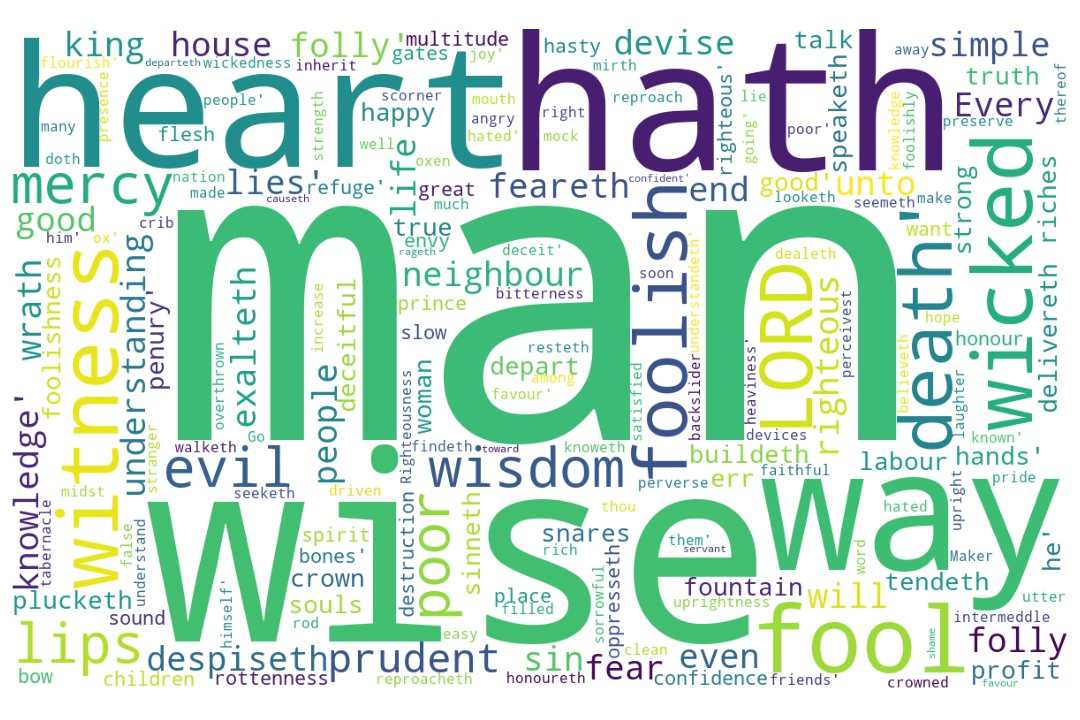
\includegraphics[width=\linewidth]{20OT-Proverbs/Proverb14-WordCloud.jpg}
  \caption{Proverb 14 Word Cloud}
  \label{fig:Proverb 14 Word Cloud}
\end{figure}

\marginpar{\scriptsize \centering \fcolorbox{bone}{lime}{\textbf{WHAT A FOOL DOES}}\\ (Proverbs 14:1-35) \begin{compactenum}[I.][8]
    \item \textbf{Derides Righteousness} (Proverbs 14:9 --  verse with 13 words) \index[scripture]{Proverbs!Pro 14:09}(Pro 14:9)
    \item \textbf{Dealeth in Anger} \index[scripture]{Proverbs!Pro 14:17}(Pro 14:17)
    \item \textbf{Despises Good} \index[scripture]{Proverbs!Pro 14:01, 21}(Pro 14:1, 21)
    \item \textbf{Devises Evil} \index[scripture]{Proverbs!Pro 14:22}(Pro 14:22)
    \item \textbf{Deceives Souls} \index[scripture]{Proverbs!Pro 14:25}(Pro 14:25)
    \item \textbf{Destroys Order} \index[scripture]{Proverbs!Pro 14:28}(Pro 14:28)
    \item \textbf{Deserves Destruction} \index[scripture]{Proverbs!Pro 14:35}(Pro 14:35)
\end{compactenum}}

\marginpar{\scriptsize \centering \fcolorbox{bone}{yellow}{\textbf{7 KINDS OF MEN}}\\ (Proverbs 14:1-35) \begin{compactenum}[I.][8]
    \item The \textbf{False} Man \index[scripture]{Proverbs!Pro 14:05}(Pro 14:5)
    \item The \textbf{Faithful} Man \index[scripture]{Proverbs!Pro 14:05}(Pro 14:5)
    \item The \textbf{Foolish} Man \index[scripture]{Proverbs!Pro 14:08} \index[scripture]{Proverbs!Pro 14:09}  \index[scripture]{Proverbs!Pro 14:24} \index[scripture]{Proverbs!Pro 14:33} (Pro 14:8, 9, 24, 33)
    \item The \textbf{Flourishing} Man \index[scripture]{Proverbs!Pro 14:11} \index[scripture]{Proverbs!Pro 14:35} (Pro 14:11, 35)
    \item The \textbf{Fearing} Man \index[scripture]{Proverbs!Pro 14:16} \index[scripture]{Proverbs!Pro 14:27} (Pro 14:16, 27)
    \item The \textbf{Fleshly} Man \index[scripture]{Proverbs!Pro 14:30} (Pro 14:30)
    \item The \textbf{Favoured} Man \index[scripture]{Proverbs!Pro 14:35} (Pro 14:35)
\end{compactenum}}

\footnote{\textcolor[cmyk]{0.99998,1,0,0}{\hyperlink{TOC}{Return to end of Table of Contents.}}}\footnote{\href{https://audiobible.com/bible/proverbs_14.html}{\textcolor[cmyk]{0.99998,1,0,0}{Proverbs Audio}}}\textcolor[cmyk]{0.99998,1,0,0}{Every wise woman buildeth her house: but the \fcolorbox{bone}{lime}{foolish plucketh it down} with her hands.}
[2] \textcolor[cmyk]{0.99998,1,0,0}{He that walketh in his uprightness feareth the LORD: but \emph{he} \emph{that} \emph{is} perverse in his ways despiseth him.}
[3] \textcolor[cmyk]{0.99998,1,0,0}{In the mouth of the foolish \emph{is} a rod of pride: but the lips of the wise shall preserve them.}
[4] \textcolor[cmyk]{0.99998,1,0,0}{Where no oxen \emph{are}, the crib \emph{is} clean: but much increase \emph{is} by the strength of the ox.}
[5] \textcolor[cmyk]{0.99998,1,0,0}{A faithful witness will not lie: but a false witness will utter lies.}
[6] \textcolor[cmyk]{0.99998,1,0,0}{A scorner seeketh wisdom, and \emph{findeth} \emph{it} not: but knowledge \emph{is} easy unto him that \fcolorbox{bone}{MYGOLD}{understandeth}.}
[7] \textcolor[cmyk]{0.99998,1,0,0}{Go from the presence of a foolish man, when thou perceivest not \emph{in} \emph{him} the lips of knowledge.}
[8] \textcolor[cmyk]{0.99998,1,0,0}{The wisdom of the prudent \emph{is} to understand his way: but the folly of fools \emph{is} deceit.}
[9] \textcolor[cmyk]{0.99998,1,0,0}{Fools make a \fcolorbox{bone}{lime}{mock at sin}: but among the righteous \emph{there} \emph{is} favour.}
[10] \textcolor[cmyk]{0.99998,1,0,0}{The heart knoweth his own bitterness; and a stranger doth not intermeddle with his joy.}
[11] \textcolor[cmyk]{0.99998,1,0,0}{The house of the wicked shall be overthrown: but the tabernacle of the upright shall flourish.}
[12] \textcolor[cmyk]{0.99998,1,0,0}{There is a way which seemeth right unto a man, but the end thereof \emph{are} the ways of death.}\footnote{\textbf{Deuteronomy 12:8} - Ye shall not do after all the things that we do here this day, every man whatsoever is right in his own eyes.}\footnote{\textbf{Judges 17:6} - In those days \emph{there} \emph{was} no king in Israel, \emph{but} every man did \emph{that} \emph{which} \emph{was} right in his own eyes.}\footnote{\textbf{Judges 21:25} - In those days \emph{there} \emph{was} no king in Israel: every man did \emph{that} \emph{which} \emph{was} right in his own eyes.}\footnote{\textbf{Proverb 21:2} - Every way of a man is right in his own eyes: but the LORD pondereth the hearts.}
[13] \textcolor[cmyk]{0.99998,1,0,0}{Even in laughter the heart is sorrowful; and the end of that mirth \emph{is} heaviness.}
[14] \textcolor[cmyk]{0.99998,1,0,0}{The backslider in heart shall be filled with his own ways: and a good man \emph{shall} \emph{be} \emph{satisfied} from himself.}
[15] \textcolor[cmyk]{0.99998,1,0,0}{The simple believeth every word: but the prudent \emph{man} looketh well to his going.}
[16] \textcolor[cmyk]{0.99998,1,0,0}{A wise \emph{man} feareth, and departeth from evil: but the fool rageth, and is confident.}
[17] \textcolor[cmyk]{0.99998,1,0,0}{\emph{He} \emph{that} \emph{is} \fcolorbox{bone}{lime}{soon angry} dealeth foolishly: and a man of wicked devices is hated.}
[18] \textcolor[cmyk]{0.99998,1,0,0}{The simple inherit folly: but the prudent are crowned with knowledge.}
[19] \textcolor[cmyk]{0.99998,1,0,0}{The evil bow before the good; and the wicked at the gates of the righteous.}
[20] \textcolor[cmyk]{0.99998,1,0,0}{The poor is hated even of his own neighbour: but the rich \emph{hath} many friends.}
[21] \textcolor[cmyk]{0.99998,1,0,0}{He that \fcolorbox{bone}{lime}{despiseth his neighbour} sinneth: but he that hath mercy on the poor, happy \emph{is} he.}
[22] \textcolor[cmyk]{0.99998,1,0,0}{Do they not err that \fcolorbox{bone}{lime}{devise evil}? but mercy and truth \emph{shall} \emph{be} to them that devise good.}
[23] \textcolor[cmyk]{0.99998,1,0,0}{In all labour there is profit: but the talk of the lips \emph{tendeth} only to penury.}
[24] \textcolor[cmyk]{0.99998,1,0,0}{The crown of the wise \emph{is} their riches: \emph{but} the foolishness of fools \emph{is} folly.}
[25] \textcolor[cmyk]{0.99998,1,0,0}{A true witness delivereth souls: but a \fcolorbox{bone}{lime}{deceitful \emph{witness}} speaketh lies.}
[26] \textcolor[cmyk]{0.99998,1,0,0}{In the fear of the LORD \emph{is} strong confidence: and his children shall have a place of refuge.}
[27] \textcolor[cmyk]{0.99998,1,0,0}{The fear of the LORD \emph{is} a fountain of life, to depart from the snares of death.}
[28] \textcolor[cmyk]{0.99998,1,0,0}{In the multitude of people \emph{is} the king's honour: but in the want of people \emph{is} the \fcolorbox{bone}{lime}{destruction of the prince}.}
[29] \textcolor[cmyk]{0.99998,1,0,0}{\emph{He} \emph{that} \emph{is} slow to wrath \emph{is} of great \fcolorbox{bone}{MYGOLD}{understanding}: but \emph{he} \emph{that} \emph{is} hasty of spirit exalteth folly.}
[30] \textcolor[cmyk]{0.99998,1,0,0}{A sound heart \emph{is} the life of the flesh: but envy the rottenness of the bones.}
[31] \textcolor[cmyk]{0.99998,1,0,0}{He that oppresseth the poor reproacheth his Maker: but he that honoureth him hath mercy on the poor.}
[32] \textcolor[cmyk]{0.99998,1,0,0}{The wicked is driven away in his wickedness: but the righteous hath hope in his death.}
[33] \textcolor[cmyk]{0.99998,1,0,0}{Wisdom resteth in the heart of him that hath \fcolorbox{bone}{MYGOLD}{understanding}: but \emph{that} \emph{which} \emph{is} in the midst of fools is made known.}
[34] \textcolor[cmyk]{0.99998,1,0,0}{\fcolorbox{bone}{MYGOLD}{Righteousness} exalteth a nation: but sin \emph{is} a reproach to any people.}
[35] \textcolor[cmyk]{0.99998,1,0,0}{The king's favour \emph{is} toward a wise servant: but his \fcolorbox{bone}{lime}{wrath is \emph{against}} him that causeth shame.}



\index[NWIV]{15!Proverbs!Pro 14:1}\index[AWIP]{Every!Proverbs!Pro 14:1}\index[AWIP]{wise!Proverbs!Pro 14:1}\index[AWIP]{woman!Proverbs!Pro 14:1}\index[AWIP]{buildeth!Proverbs!Pro 14:1}\index[AWIP]{her!Proverbs!Pro 14:1}\index[AWIP]{her!Proverbs!Pro 14:1 (2)}\index[AWIP]{house!Proverbs!Pro 14:1}\index[AWIP]{but!Proverbs!Pro 14:1}\index[AWIP]{the!Proverbs!Pro 14:1}\index[AWIP]{foolish!Proverbs!Pro 14:1}\index[AWIP]{plucketh!Proverbs!Pro 14:1}\index[AWIP]{it!Proverbs!Pro 14:1}\index[AWIP]{down!Proverbs!Pro 14:1}\index[AWIP]{with!Proverbs!Pro 14:1}\index[AWIP]{hands!Proverbs!Pro 14:1}

\index[NWIV]{19!Proverbs!Pro 14:2}\index[AWIP]{He!Proverbs!Pro 14:2}\index[AWIP]{that!Proverbs!Pro 14:2}\index[AWIP]{walketh!Proverbs!Pro 14:2}\index[AWIP]{in!Proverbs!Pro 14:2}\index[AWIP]{in!Proverbs!Pro 14:2 (2)}\index[AWIP]{his!Proverbs!Pro 14:2}\index[AWIP]{his!Proverbs!Pro 14:2 (2)}\index[AWIP]{uprightness!Proverbs!Pro 14:2}\index[AWIP]{feareth!Proverbs!Pro 14:2}\index[AWIP]{the!Proverbs!Pro 14:2}\index[AWIP]{LORD!Proverbs!Pro 14:2}\index[AWIP]{but!Proverbs!Pro 14:2}\index[AWIP]{\emph{he}!Proverbs!Pro 14:2}\index[AWIP]{\emph{that}!Proverbs!Pro 14:2}\index[AWIP]{\emph{is}!Proverbs!Pro 14:2}\index[AWIP]{perverse!Proverbs!Pro 14:2}\index[AWIP]{ways!Proverbs!Pro 14:2}\index[AWIP]{despiseth!Proverbs!Pro 14:2}\index[AWIP]{him!Proverbs!Pro 14:2}\index[AWIP]{\emph{he}!Proverbs!Pro 14:2}\index[AWIP]{\emph{that}!Proverbs!Pro 14:2}\index[AWIP]{\emph{is}!Proverbs!Pro 14:2}

\index[NWIV]{20!Proverbs!Pro 14:3}\index[AWIP]{In!Proverbs!Pro 14:3}\index[AWIP]{the!Proverbs!Pro 14:3}\index[AWIP]{the!Proverbs!Pro 14:3 (2)}\index[AWIP]{the!Proverbs!Pro 14:3 (3)}\index[AWIP]{the!Proverbs!Pro 14:3 (4)}\index[AWIP]{mouth!Proverbs!Pro 14:3}\index[AWIP]{of!Proverbs!Pro 14:3}\index[AWIP]{of!Proverbs!Pro 14:3 (2)}\index[AWIP]{of!Proverbs!Pro 14:3 (3)}\index[AWIP]{foolish!Proverbs!Pro 14:3}\index[AWIP]{\emph{is}!Proverbs!Pro 14:3}\index[AWIP]{a!Proverbs!Pro 14:3}\index[AWIP]{rod!Proverbs!Pro 14:3}\index[AWIP]{pride!Proverbs!Pro 14:3}\index[AWIP]{but!Proverbs!Pro 14:3}\index[AWIP]{lips!Proverbs!Pro 14:3}\index[AWIP]{wise!Proverbs!Pro 14:3}\index[AWIP]{shall!Proverbs!Pro 14:3}\index[AWIP]{preserve!Proverbs!Pro 14:3}\index[AWIP]{them!Proverbs!Pro 14:3}\index[AWIP]{\emph{is}!Proverbs!Pro 14:3}

\index[NWIV]{18!Proverbs!Pro 14:4}\index[AWIP]{Where!Proverbs!Pro 14:4}\index[AWIP]{no!Proverbs!Pro 14:4}\index[AWIP]{oxen!Proverbs!Pro 14:4}\index[AWIP]{\emph{are}!Proverbs!Pro 14:4}\index[AWIP]{the!Proverbs!Pro 14:4}\index[AWIP]{the!Proverbs!Pro 14:4 (2)}\index[AWIP]{the!Proverbs!Pro 14:4 (3)}\index[AWIP]{crib!Proverbs!Pro 14:4}\index[AWIP]{\emph{is}!Proverbs!Pro 14:4}\index[AWIP]{\emph{is}!Proverbs!Pro 14:4 (2)}\index[AWIP]{clean!Proverbs!Pro 14:4}\index[AWIP]{but!Proverbs!Pro 14:4}\index[AWIP]{much!Proverbs!Pro 14:4}\index[AWIP]{increase!Proverbs!Pro 14:4}\index[AWIP]{by!Proverbs!Pro 14:4}\index[AWIP]{strength!Proverbs!Pro 14:4}\index[AWIP]{of!Proverbs!Pro 14:4}\index[AWIP]{ox!Proverbs!Pro 14:4}\index[AWIP]{\emph{are}!Proverbs!Pro 14:4}\index[AWIP]{\emph{is}!Proverbs!Pro 14:4}\index[AWIP]{\emph{is}!Proverbs!Pro 14:4 (2)}

\index[NWIV]{13!Proverbs!Pro 14:5}\index[AWIP]{A!Proverbs!Pro 14:5}\index[AWIP]{faithful!Proverbs!Pro 14:5}\index[AWIP]{witness!Proverbs!Pro 14:5}\index[AWIP]{witness!Proverbs!Pro 14:5 (2)}\index[AWIP]{will!Proverbs!Pro 14:5}\index[AWIP]{will!Proverbs!Pro 14:5 (2)}\index[AWIP]{not!Proverbs!Pro 14:5}\index[AWIP]{lie!Proverbs!Pro 14:5}\index[AWIP]{but!Proverbs!Pro 14:5}\index[AWIP]{a!Proverbs!Pro 14:5}\index[AWIP]{false!Proverbs!Pro 14:5}\index[AWIP]{utter!Proverbs!Pro 14:5}\index[AWIP]{lies!Proverbs!Pro 14:5}

\index[NWIV]{16!Proverbs!Pro 14:6}\index[AWIP]{A!Proverbs!Pro 14:6}\index[AWIP]{scorner!Proverbs!Pro 14:6}\index[AWIP]{seeketh!Proverbs!Pro 14:6}\index[AWIP]{wisdom!Proverbs!Pro 14:6}\index[AWIP]{and!Proverbs!Pro 14:6}\index[AWIP]{\emph{findeth}!Proverbs!Pro 14:6}\index[AWIP]{\emph{it}!Proverbs!Pro 14:6}\index[AWIP]{not!Proverbs!Pro 14:6}\index[AWIP]{but!Proverbs!Pro 14:6}\index[AWIP]{knowledge!Proverbs!Pro 14:6}\index[AWIP]{\emph{is}!Proverbs!Pro 14:6}\index[AWIP]{easy!Proverbs!Pro 14:6}\index[AWIP]{unto!Proverbs!Pro 14:6}\index[AWIP]{him!Proverbs!Pro 14:6}\index[AWIP]{that!Proverbs!Pro 14:6}\index[AWIP]{understandeth!Proverbs!Pro 14:6}\index[AWIP]{\emph{findeth}!Proverbs!Pro 14:6}\index[AWIP]{\emph{it}!Proverbs!Pro 14:6}\index[AWIP]{\emph{is}!Proverbs!Pro 14:6}

\index[NWIV]{18!Proverbs!Pro 14:7}\index[AWIP]{Go!Proverbs!Pro 14:7}\index[AWIP]{from!Proverbs!Pro 14:7}\index[AWIP]{the!Proverbs!Pro 14:7}\index[AWIP]{the!Proverbs!Pro 14:7 (2)}\index[AWIP]{presence!Proverbs!Pro 14:7}\index[AWIP]{of!Proverbs!Pro 14:7}\index[AWIP]{of!Proverbs!Pro 14:7 (2)}\index[AWIP]{a!Proverbs!Pro 14:7}\index[AWIP]{foolish!Proverbs!Pro 14:7}\index[AWIP]{man!Proverbs!Pro 14:7}\index[AWIP]{when!Proverbs!Pro 14:7}\index[AWIP]{thou!Proverbs!Pro 14:7}\index[AWIP]{perceivest!Proverbs!Pro 14:7}\index[AWIP]{not!Proverbs!Pro 14:7}\index[AWIP]{\emph{in}!Proverbs!Pro 14:7}\index[AWIP]{\emph{him}!Proverbs!Pro 14:7}\index[AWIP]{lips!Proverbs!Pro 14:7}\index[AWIP]{knowledge!Proverbs!Pro 14:7}\index[AWIP]{\emph{in}!Proverbs!Pro 14:7}\index[AWIP]{\emph{him}!Proverbs!Pro 14:7}

\index[NWIV]{17!Proverbs!Pro 14:8}\index[AWIP]{The!Proverbs!Pro 14:8}\index[AWIP]{wisdom!Proverbs!Pro 14:8}\index[AWIP]{of!Proverbs!Pro 14:8}\index[AWIP]{of!Proverbs!Pro 14:8 (2)}\index[AWIP]{the!Proverbs!Pro 14:8}\index[AWIP]{the!Proverbs!Pro 14:8 (2)}\index[AWIP]{prudent!Proverbs!Pro 14:8}\index[AWIP]{\emph{is}!Proverbs!Pro 14:8}\index[AWIP]{\emph{is}!Proverbs!Pro 14:8 (2)}\index[AWIP]{to!Proverbs!Pro 14:8}\index[AWIP]{understand!Proverbs!Pro 14:8}\index[AWIP]{his!Proverbs!Pro 14:8}\index[AWIP]{way!Proverbs!Pro 14:8}\index[AWIP]{but!Proverbs!Pro 14:8}\index[AWIP]{folly!Proverbs!Pro 14:8}\index[AWIP]{fools!Proverbs!Pro 14:8}\index[AWIP]{deceit!Proverbs!Pro 14:8}\index[AWIP]{\emph{is}!Proverbs!Pro 14:8}\index[AWIP]{\emph{is}!Proverbs!Pro 14:8 (2)}

\index[NWIV]{13!Proverbs!Pro 14:9}\index[AWIP]{Fools!Proverbs!Pro 14:9}\index[AWIP]{make!Proverbs!Pro 14:9}\index[AWIP]{a!Proverbs!Pro 14:9}\index[AWIP]{mock!Proverbs!Pro 14:9}\index[AWIP]{at!Proverbs!Pro 14:9}\index[AWIP]{sin!Proverbs!Pro 14:9}\index[AWIP]{but!Proverbs!Pro 14:9}\index[AWIP]{among!Proverbs!Pro 14:9}\index[AWIP]{the!Proverbs!Pro 14:9}\index[AWIP]{righteous!Proverbs!Pro 14:9}\index[AWIP]{\emph{there}!Proverbs!Pro 14:9}\index[AWIP]{\emph{is}!Proverbs!Pro 14:9}\index[AWIP]{favour!Proverbs!Pro 14:9}\index[AWIP]{\emph{there}!Proverbs!Pro 14:9}\index[AWIP]{\emph{is}!Proverbs!Pro 14:9}

\index[NWIV]{15!Proverbs!Pro 14:10}\index[AWIP]{The!Proverbs!Pro 14:10}\index[AWIP]{heart!Proverbs!Pro 14:10}\index[AWIP]{knoweth!Proverbs!Pro 14:10}\index[AWIP]{his!Proverbs!Pro 14:10}\index[AWIP]{his!Proverbs!Pro 14:10 (2)}\index[AWIP]{own!Proverbs!Pro 14:10}\index[AWIP]{bitterness!Proverbs!Pro 14:10}\index[AWIP]{and!Proverbs!Pro 14:10}\index[AWIP]{a!Proverbs!Pro 14:10}\index[AWIP]{stranger!Proverbs!Pro 14:10}\index[AWIP]{doth!Proverbs!Pro 14:10}\index[AWIP]{not!Proverbs!Pro 14:10}\index[AWIP]{intermeddle!Proverbs!Pro 14:10}\index[AWIP]{with!Proverbs!Pro 14:10}\index[AWIP]{joy!Proverbs!Pro 14:10}

\index[NWIV]{16!Proverbs!Pro 14:11}\index[AWIP]{The!Proverbs!Pro 14:11}\index[AWIP]{house!Proverbs!Pro 14:11}\index[AWIP]{of!Proverbs!Pro 14:11}\index[AWIP]{of!Proverbs!Pro 14:11 (2)}\index[AWIP]{the!Proverbs!Pro 14:11}\index[AWIP]{the!Proverbs!Pro 14:11 (2)}\index[AWIP]{the!Proverbs!Pro 14:11 (3)}\index[AWIP]{wicked!Proverbs!Pro 14:11}\index[AWIP]{shall!Proverbs!Pro 14:11}\index[AWIP]{shall!Proverbs!Pro 14:11 (2)}\index[AWIP]{be!Proverbs!Pro 14:11}\index[AWIP]{overthrown!Proverbs!Pro 14:11}\index[AWIP]{but!Proverbs!Pro 14:11}\index[AWIP]{tabernacle!Proverbs!Pro 14:11}\index[AWIP]{upright!Proverbs!Pro 14:11}\index[AWIP]{flourish!Proverbs!Pro 14:11}

\index[NWIV]{19!Proverbs!Pro 14:12}\index[AWIP]{There!Proverbs!Pro 14:12}\index[AWIP]{is!Proverbs!Pro 14:12}\index[AWIP]{a!Proverbs!Pro 14:12}\index[AWIP]{a!Proverbs!Pro 14:12 (2)}\index[AWIP]{way!Proverbs!Pro 14:12}\index[AWIP]{which!Proverbs!Pro 14:12}\index[AWIP]{seemeth!Proverbs!Pro 14:12}\index[AWIP]{right!Proverbs!Pro 14:12}\index[AWIP]{unto!Proverbs!Pro 14:12}\index[AWIP]{man!Proverbs!Pro 14:12}\index[AWIP]{but!Proverbs!Pro 14:12}\index[AWIP]{the!Proverbs!Pro 14:12}\index[AWIP]{the!Proverbs!Pro 14:12 (2)}\index[AWIP]{end!Proverbs!Pro 14:12}\index[AWIP]{thereof!Proverbs!Pro 14:12}\index[AWIP]{\emph{are}!Proverbs!Pro 14:12}\index[AWIP]{ways!Proverbs!Pro 14:12}\index[AWIP]{of!Proverbs!Pro 14:12}\index[AWIP]{death!Proverbs!Pro 14:12}\index[AWIP]{\emph{are}!Proverbs!Pro 14:12}

\index[NWIV]{15!Proverbs!Pro 14:13}\index[AWIP]{Even!Proverbs!Pro 14:13}\index[AWIP]{in!Proverbs!Pro 14:13}\index[AWIP]{laughter!Proverbs!Pro 14:13}\index[AWIP]{the!Proverbs!Pro 14:13}\index[AWIP]{the!Proverbs!Pro 14:13 (2)}\index[AWIP]{heart!Proverbs!Pro 14:13}\index[AWIP]{is!Proverbs!Pro 14:13}\index[AWIP]{sorrowful!Proverbs!Pro 14:13}\index[AWIP]{and!Proverbs!Pro 14:13}\index[AWIP]{end!Proverbs!Pro 14:13}\index[AWIP]{of!Proverbs!Pro 14:13}\index[AWIP]{that!Proverbs!Pro 14:13}\index[AWIP]{mirth!Proverbs!Pro 14:13}\index[AWIP]{\emph{is}!Proverbs!Pro 14:13}\index[AWIP]{heaviness!Proverbs!Pro 14:13}\index[AWIP]{\emph{is}!Proverbs!Pro 14:13}

\index[NWIV]{20!Proverbs!Pro 14:14}\index[AWIP]{The!Proverbs!Pro 14:14}\index[AWIP]{backslider!Proverbs!Pro 14:14}\index[AWIP]{in!Proverbs!Pro 14:14}\index[AWIP]{heart!Proverbs!Pro 14:14}\index[AWIP]{shall!Proverbs!Pro 14:14}\index[AWIP]{be!Proverbs!Pro 14:14}\index[AWIP]{filled!Proverbs!Pro 14:14}\index[AWIP]{with!Proverbs!Pro 14:14}\index[AWIP]{his!Proverbs!Pro 14:14}\index[AWIP]{own!Proverbs!Pro 14:14}\index[AWIP]{ways!Proverbs!Pro 14:14}\index[AWIP]{and!Proverbs!Pro 14:14}\index[AWIP]{a!Proverbs!Pro 14:14}\index[AWIP]{good!Proverbs!Pro 14:14}\index[AWIP]{man!Proverbs!Pro 14:14}\index[AWIP]{\emph{shall}!Proverbs!Pro 14:14}\index[AWIP]{\emph{be}!Proverbs!Pro 14:14}\index[AWIP]{\emph{satisfied}!Proverbs!Pro 14:14}\index[AWIP]{from!Proverbs!Pro 14:14}\index[AWIP]{himself!Proverbs!Pro 14:14}\index[AWIP]{\emph{shall}!Proverbs!Pro 14:14}\index[AWIP]{\emph{be}!Proverbs!Pro 14:14}\index[AWIP]{\emph{satisfied}!Proverbs!Pro 14:14}

\index[NWIV]{14!Proverbs!Pro 14:15}\index[AWIP]{The!Proverbs!Pro 14:15}\index[AWIP]{simple!Proverbs!Pro 14:15}\index[AWIP]{believeth!Proverbs!Pro 14:15}\index[AWIP]{every!Proverbs!Pro 14:15}\index[AWIP]{word!Proverbs!Pro 14:15}\index[AWIP]{but!Proverbs!Pro 14:15}\index[AWIP]{the!Proverbs!Pro 14:15}\index[AWIP]{prudent!Proverbs!Pro 14:15}\index[AWIP]{\emph{man}!Proverbs!Pro 14:15}\index[AWIP]{looketh!Proverbs!Pro 14:15}\index[AWIP]{well!Proverbs!Pro 14:15}\index[AWIP]{to!Proverbs!Pro 14:15}\index[AWIP]{his!Proverbs!Pro 14:15}\index[AWIP]{going!Proverbs!Pro 14:15}\index[AWIP]{\emph{man}!Proverbs!Pro 14:15}

\index[NWIV]{15!Proverbs!Pro 14:16}\index[AWIP]{A!Proverbs!Pro 14:16}\index[AWIP]{wise!Proverbs!Pro 14:16}\index[AWIP]{\emph{man}!Proverbs!Pro 14:16}\index[AWIP]{feareth!Proverbs!Pro 14:16}\index[AWIP]{and!Proverbs!Pro 14:16}\index[AWIP]{and!Proverbs!Pro 14:16 (2)}\index[AWIP]{departeth!Proverbs!Pro 14:16}\index[AWIP]{from!Proverbs!Pro 14:16}\index[AWIP]{evil!Proverbs!Pro 14:16}\index[AWIP]{but!Proverbs!Pro 14:16}\index[AWIP]{the!Proverbs!Pro 14:16}\index[AWIP]{fool!Proverbs!Pro 14:16}\index[AWIP]{rageth!Proverbs!Pro 14:16}\index[AWIP]{is!Proverbs!Pro 14:16}\index[AWIP]{confident!Proverbs!Pro 14:16}\index[AWIP]{\emph{man}!Proverbs!Pro 14:16}

\index[NWIV]{15!Proverbs!Pro 14:17}\index[AWIP]{\emph{He}!Proverbs!Pro 14:17}\index[AWIP]{\emph{that}!Proverbs!Pro 14:17}\index[AWIP]{\emph{is}!Proverbs!Pro 14:17}\index[AWIP]{soon!Proverbs!Pro 14:17}\index[AWIP]{angry!Proverbs!Pro 14:17}\index[AWIP]{dealeth!Proverbs!Pro 14:17}\index[AWIP]{foolishly!Proverbs!Pro 14:17}\index[AWIP]{and!Proverbs!Pro 14:17}\index[AWIP]{a!Proverbs!Pro 14:17}\index[AWIP]{man!Proverbs!Pro 14:17}\index[AWIP]{of!Proverbs!Pro 14:17}\index[AWIP]{wicked!Proverbs!Pro 14:17}\index[AWIP]{devices!Proverbs!Pro 14:17}\index[AWIP]{is!Proverbs!Pro 14:17}\index[AWIP]{hated!Proverbs!Pro 14:17}\index[AWIP]{\emph{He}!Proverbs!Pro 14:17}\index[AWIP]{\emph{that}!Proverbs!Pro 14:17}\index[AWIP]{\emph{is}!Proverbs!Pro 14:17}

\index[NWIV]{11!Proverbs!Pro 14:18}\index[AWIP]{The!Proverbs!Pro 14:18}\index[AWIP]{simple!Proverbs!Pro 14:18}\index[AWIP]{inherit!Proverbs!Pro 14:18}\index[AWIP]{folly!Proverbs!Pro 14:18}\index[AWIP]{but!Proverbs!Pro 14:18}\index[AWIP]{the!Proverbs!Pro 14:18}\index[AWIP]{prudent!Proverbs!Pro 14:18}\index[AWIP]{are!Proverbs!Pro 14:18}\index[AWIP]{crowned!Proverbs!Pro 14:18}\index[AWIP]{with!Proverbs!Pro 14:18}\index[AWIP]{knowledge!Proverbs!Pro 14:18}

\index[NWIV]{15!Proverbs!Pro 14:19}\index[AWIP]{The!Proverbs!Pro 14:19}\index[AWIP]{evil!Proverbs!Pro 14:19}\index[AWIP]{bow!Proverbs!Pro 14:19}\index[AWIP]{before!Proverbs!Pro 14:19}\index[AWIP]{the!Proverbs!Pro 14:19}\index[AWIP]{the!Proverbs!Pro 14:19 (2)}\index[AWIP]{the!Proverbs!Pro 14:19 (3)}\index[AWIP]{the!Proverbs!Pro 14:19 (4)}\index[AWIP]{good!Proverbs!Pro 14:19}\index[AWIP]{and!Proverbs!Pro 14:19}\index[AWIP]{wicked!Proverbs!Pro 14:19}\index[AWIP]{at!Proverbs!Pro 14:19}\index[AWIP]{gates!Proverbs!Pro 14:19}\index[AWIP]{of!Proverbs!Pro 14:19}\index[AWIP]{righteous!Proverbs!Pro 14:19}

\index[NWIV]{15!Proverbs!Pro 14:20}\index[AWIP]{The!Proverbs!Pro 14:20}\index[AWIP]{poor!Proverbs!Pro 14:20}\index[AWIP]{is!Proverbs!Pro 14:20}\index[AWIP]{hated!Proverbs!Pro 14:20}\index[AWIP]{even!Proverbs!Pro 14:20}\index[AWIP]{of!Proverbs!Pro 14:20}\index[AWIP]{his!Proverbs!Pro 14:20}\index[AWIP]{own!Proverbs!Pro 14:20}\index[AWIP]{neighbour!Proverbs!Pro 14:20}\index[AWIP]{but!Proverbs!Pro 14:20}\index[AWIP]{the!Proverbs!Pro 14:20}\index[AWIP]{rich!Proverbs!Pro 14:20}\index[AWIP]{\emph{hath}!Proverbs!Pro 14:20}\index[AWIP]{many!Proverbs!Pro 14:20}\index[AWIP]{friends!Proverbs!Pro 14:20}\index[AWIP]{\emph{hath}!Proverbs!Pro 14:20}

\index[NWIV]{17!Proverbs!Pro 14:21}\index[AWIP]{He!Proverbs!Pro 14:21}\index[AWIP]{that!Proverbs!Pro 14:21}\index[AWIP]{that!Proverbs!Pro 14:21 (2)}\index[AWIP]{despiseth!Proverbs!Pro 14:21}\index[AWIP]{his!Proverbs!Pro 14:21}\index[AWIP]{neighbour!Proverbs!Pro 14:21}\index[AWIP]{sinneth!Proverbs!Pro 14:21}\index[AWIP]{but!Proverbs!Pro 14:21}\index[AWIP]{he!Proverbs!Pro 14:21}\index[AWIP]{he!Proverbs!Pro 14:21 (2)}\index[AWIP]{hath!Proverbs!Pro 14:21}\index[AWIP]{mercy!Proverbs!Pro 14:21}\index[AWIP]{on!Proverbs!Pro 14:21}\index[AWIP]{the!Proverbs!Pro 14:21}\index[AWIP]{poor!Proverbs!Pro 14:21}\index[AWIP]{happy!Proverbs!Pro 14:21}\index[AWIP]{\emph{is}!Proverbs!Pro 14:21}\index[AWIP]{\emph{is}!Proverbs!Pro 14:21}

\index[NWIV]{18!Proverbs!Pro 14:22}\index[AWIP]{Do!Proverbs!Pro 14:22}\index[AWIP]{they!Proverbs!Pro 14:22}\index[AWIP]{not!Proverbs!Pro 14:22}\index[AWIP]{err!Proverbs!Pro 14:22}\index[AWIP]{that!Proverbs!Pro 14:22}\index[AWIP]{that!Proverbs!Pro 14:22 (2)}\index[AWIP]{devise!Proverbs!Pro 14:22}\index[AWIP]{devise!Proverbs!Pro 14:22 (2)}\index[AWIP]{evil?!Proverbs!Pro 14:22}\index[AWIP]{but!Proverbs!Pro 14:22}\index[AWIP]{mercy!Proverbs!Pro 14:22}\index[AWIP]{and!Proverbs!Pro 14:22}\index[AWIP]{truth!Proverbs!Pro 14:22}\index[AWIP]{\emph{shall}!Proverbs!Pro 14:22}\index[AWIP]{\emph{be}!Proverbs!Pro 14:22}\index[AWIP]{to!Proverbs!Pro 14:22}\index[AWIP]{them!Proverbs!Pro 14:22}\index[AWIP]{good!Proverbs!Pro 14:22}\index[AWIP]{\emph{shall}!Proverbs!Pro 14:22}\index[AWIP]{\emph{be}!Proverbs!Pro 14:22}

\index[NWIV]{16!Proverbs!Pro 14:23}\index[AWIP]{In!Proverbs!Pro 14:23}\index[AWIP]{all!Proverbs!Pro 14:23}\index[AWIP]{labour!Proverbs!Pro 14:23}\index[AWIP]{there!Proverbs!Pro 14:23}\index[AWIP]{is!Proverbs!Pro 14:23}\index[AWIP]{profit!Proverbs!Pro 14:23}\index[AWIP]{but!Proverbs!Pro 14:23}\index[AWIP]{the!Proverbs!Pro 14:23}\index[AWIP]{the!Proverbs!Pro 14:23 (2)}\index[AWIP]{talk!Proverbs!Pro 14:23}\index[AWIP]{of!Proverbs!Pro 14:23}\index[AWIP]{lips!Proverbs!Pro 14:23}\index[AWIP]{\emph{tendeth}!Proverbs!Pro 14:23}\index[AWIP]{only!Proverbs!Pro 14:23}\index[AWIP]{to!Proverbs!Pro 14:23}\index[AWIP]{penury!Proverbs!Pro 14:23}\index[AWIP]{\emph{tendeth}!Proverbs!Pro 14:23}

\index[NWIV]{15!Proverbs!Pro 14:24}\index[AWIP]{The!Proverbs!Pro 14:24}\index[AWIP]{crown!Proverbs!Pro 14:24}\index[AWIP]{of!Proverbs!Pro 14:24}\index[AWIP]{of!Proverbs!Pro 14:24 (2)}\index[AWIP]{the!Proverbs!Pro 14:24}\index[AWIP]{the!Proverbs!Pro 14:24 (2)}\index[AWIP]{wise!Proverbs!Pro 14:24}\index[AWIP]{\emph{is}!Proverbs!Pro 14:24}\index[AWIP]{\emph{is}!Proverbs!Pro 14:24 (2)}\index[AWIP]{their!Proverbs!Pro 14:24}\index[AWIP]{riches!Proverbs!Pro 14:24}\index[AWIP]{\emph{but}!Proverbs!Pro 14:24}\index[AWIP]{foolishness!Proverbs!Pro 14:24}\index[AWIP]{fools!Proverbs!Pro 14:24}\index[AWIP]{folly!Proverbs!Pro 14:24}\index[AWIP]{\emph{is}!Proverbs!Pro 14:24}\index[AWIP]{\emph{is}!Proverbs!Pro 14:24 (2)}\index[AWIP]{\emph{but}!Proverbs!Pro 14:24}

\index[NWIV]{11!Proverbs!Pro 14:25}\index[AWIP]{A!Proverbs!Pro 14:25}\index[AWIP]{true!Proverbs!Pro 14:25}\index[AWIP]{witness!Proverbs!Pro 14:25}\index[AWIP]{delivereth!Proverbs!Pro 14:25}\index[AWIP]{souls!Proverbs!Pro 14:25}\index[AWIP]{but!Proverbs!Pro 14:25}\index[AWIP]{a!Proverbs!Pro 14:25}\index[AWIP]{deceitful!Proverbs!Pro 14:25}\index[AWIP]{\emph{witness}!Proverbs!Pro 14:25}\index[AWIP]{speaketh!Proverbs!Pro 14:25}\index[AWIP]{lies!Proverbs!Pro 14:25}\index[AWIP]{\emph{witness}!Proverbs!Pro 14:25}

\index[NWIV]{18!Proverbs!Pro 14:26}\index[AWIP]{In!Proverbs!Pro 14:26}\index[AWIP]{the!Proverbs!Pro 14:26}\index[AWIP]{the!Proverbs!Pro 14:26 (2)}\index[AWIP]{fear!Proverbs!Pro 14:26}\index[AWIP]{of!Proverbs!Pro 14:26}\index[AWIP]{of!Proverbs!Pro 14:26 (2)}\index[AWIP]{LORD!Proverbs!Pro 14:26}\index[AWIP]{\emph{is}!Proverbs!Pro 14:26}\index[AWIP]{strong!Proverbs!Pro 14:26}\index[AWIP]{confidence!Proverbs!Pro 14:26}\index[AWIP]{and!Proverbs!Pro 14:26}\index[AWIP]{his!Proverbs!Pro 14:26}\index[AWIP]{children!Proverbs!Pro 14:26}\index[AWIP]{shall!Proverbs!Pro 14:26}\index[AWIP]{have!Proverbs!Pro 14:26}\index[AWIP]{a!Proverbs!Pro 14:26}\index[AWIP]{place!Proverbs!Pro 14:26}\index[AWIP]{refuge!Proverbs!Pro 14:26}\index[AWIP]{\emph{is}!Proverbs!Pro 14:26}

\index[NWIV]{17!Proverbs!Pro 14:27}\index[AWIP]{The!Proverbs!Pro 14:27}\index[AWIP]{fear!Proverbs!Pro 14:27}\index[AWIP]{of!Proverbs!Pro 14:27}\index[AWIP]{of!Proverbs!Pro 14:27 (2)}\index[AWIP]{of!Proverbs!Pro 14:27 (3)}\index[AWIP]{the!Proverbs!Pro 14:27}\index[AWIP]{the!Proverbs!Pro 14:27 (2)}\index[AWIP]{LORD!Proverbs!Pro 14:27}\index[AWIP]{\emph{is}!Proverbs!Pro 14:27}\index[AWIP]{a!Proverbs!Pro 14:27}\index[AWIP]{fountain!Proverbs!Pro 14:27}\index[AWIP]{life!Proverbs!Pro 14:27}\index[AWIP]{to!Proverbs!Pro 14:27}\index[AWIP]{depart!Proverbs!Pro 14:27}\index[AWIP]{from!Proverbs!Pro 14:27}\index[AWIP]{snares!Proverbs!Pro 14:27}\index[AWIP]{death!Proverbs!Pro 14:27}\index[AWIP]{\emph{is}!Proverbs!Pro 14:27}

\index[NWIV]{21!Proverbs!Pro 14:28}\index[AWIP]{In!Proverbs!Pro 14:28}\index[AWIP]{the!Proverbs!Pro 14:28}\index[AWIP]{the!Proverbs!Pro 14:28 (2)}\index[AWIP]{the!Proverbs!Pro 14:28 (3)}\index[AWIP]{the!Proverbs!Pro 14:28 (4)}\index[AWIP]{the!Proverbs!Pro 14:28 (5)}\index[AWIP]{multitude!Proverbs!Pro 14:28}\index[AWIP]{of!Proverbs!Pro 14:28}\index[AWIP]{of!Proverbs!Pro 14:28 (2)}\index[AWIP]{of!Proverbs!Pro 14:28 (3)}\index[AWIP]{people!Proverbs!Pro 14:28}\index[AWIP]{people!Proverbs!Pro 14:28 (2)}\index[AWIP]{\emph{is}!Proverbs!Pro 14:28}\index[AWIP]{\emph{is}!Proverbs!Pro 14:28 (2)}\index[AWIP]{king's!Proverbs!Pro 14:28}\index[AWIP]{honour!Proverbs!Pro 14:28}\index[AWIP]{but!Proverbs!Pro 14:28}\index[AWIP]{in!Proverbs!Pro 14:28}\index[AWIP]{want!Proverbs!Pro 14:28}\index[AWIP]{destruction!Proverbs!Pro 14:28}\index[AWIP]{prince!Proverbs!Pro 14:28}\index[AWIP]{\emph{is}!Proverbs!Pro 14:28}\index[AWIP]{\emph{is}!Proverbs!Pro 14:28 (2)}

\index[NWIV]{19!Proverbs!Pro 14:29}\index[AWIP]{\emph{He}!Proverbs!Pro 14:29}\index[AWIP]{\emph{that}!Proverbs!Pro 14:29}\index[AWIP]{\emph{that}!Proverbs!Pro 14:29 (2)}\index[AWIP]{\emph{is}!Proverbs!Pro 14:29}\index[AWIP]{\emph{is}!Proverbs!Pro 14:29 (2)}\index[AWIP]{\emph{is}!Proverbs!Pro 14:29 (3)}\index[AWIP]{slow!Proverbs!Pro 14:29}\index[AWIP]{to!Proverbs!Pro 14:29}\index[AWIP]{wrath!Proverbs!Pro 14:29}\index[AWIP]{of!Proverbs!Pro 14:29}\index[AWIP]{of!Proverbs!Pro 14:29 (2)}\index[AWIP]{great!Proverbs!Pro 14:29}\index[AWIP]{understanding!Proverbs!Pro 14:29}\index[AWIP]{but!Proverbs!Pro 14:29}\index[AWIP]{\emph{he}!Proverbs!Pro 14:29}\index[AWIP]{hasty!Proverbs!Pro 14:29}\index[AWIP]{spirit!Proverbs!Pro 14:29}\index[AWIP]{exalteth!Proverbs!Pro 14:29}\index[AWIP]{folly!Proverbs!Pro 14:29}\index[AWIP]{\emph{He}!Proverbs!Pro 14:29}\index[AWIP]{\emph{that}!Proverbs!Pro 14:29}\index[AWIP]{\emph{that}!Proverbs!Pro 14:29 (2)}\index[AWIP]{\emph{is}!Proverbs!Pro 14:29}\index[AWIP]{\emph{is}!Proverbs!Pro 14:29 (2)}\index[AWIP]{\emph{is}!Proverbs!Pro 14:29 (3)}\index[AWIP]{\emph{he}!Proverbs!Pro 14:29}

\index[NWIV]{16!Proverbs!Pro 14:30}\index[AWIP]{A!Proverbs!Pro 14:30}\index[AWIP]{sound!Proverbs!Pro 14:30}\index[AWIP]{heart!Proverbs!Pro 14:30}\index[AWIP]{\emph{is}!Proverbs!Pro 14:30}\index[AWIP]{the!Proverbs!Pro 14:30}\index[AWIP]{the!Proverbs!Pro 14:30 (2)}\index[AWIP]{the!Proverbs!Pro 14:30 (3)}\index[AWIP]{the!Proverbs!Pro 14:30 (4)}\index[AWIP]{life!Proverbs!Pro 14:30}\index[AWIP]{of!Proverbs!Pro 14:30}\index[AWIP]{of!Proverbs!Pro 14:30 (2)}\index[AWIP]{flesh!Proverbs!Pro 14:30}\index[AWIP]{but!Proverbs!Pro 14:30}\index[AWIP]{envy!Proverbs!Pro 14:30}\index[AWIP]{rottenness!Proverbs!Pro 14:30}\index[AWIP]{bones!Proverbs!Pro 14:30}\index[AWIP]{\emph{is}!Proverbs!Pro 14:30}

\index[NWIV]{18!Proverbs!Pro 14:31}\index[AWIP]{He!Proverbs!Pro 14:31}\index[AWIP]{that!Proverbs!Pro 14:31}\index[AWIP]{that!Proverbs!Pro 14:31 (2)}\index[AWIP]{oppresseth!Proverbs!Pro 14:31}\index[AWIP]{the!Proverbs!Pro 14:31}\index[AWIP]{the!Proverbs!Pro 14:31 (2)}\index[AWIP]{poor!Proverbs!Pro 14:31}\index[AWIP]{poor!Proverbs!Pro 14:31 (2)}\index[AWIP]{reproacheth!Proverbs!Pro 14:31}\index[AWIP]{his!Proverbs!Pro 14:31}\index[AWIP]{Maker!Proverbs!Pro 14:31}\index[AWIP]{but!Proverbs!Pro 14:31}\index[AWIP]{he!Proverbs!Pro 14:31}\index[AWIP]{honoureth!Proverbs!Pro 14:31}\index[AWIP]{him!Proverbs!Pro 14:31}\index[AWIP]{hath!Proverbs!Pro 14:31}\index[AWIP]{mercy!Proverbs!Pro 14:31}\index[AWIP]{on!Proverbs!Pro 14:31}

\index[NWIV]{16!Proverbs!Pro 14:32}\index[AWIP]{The!Proverbs!Pro 14:32}\index[AWIP]{wicked!Proverbs!Pro 14:32}\index[AWIP]{is!Proverbs!Pro 14:32}\index[AWIP]{driven!Proverbs!Pro 14:32}\index[AWIP]{away!Proverbs!Pro 14:32}\index[AWIP]{in!Proverbs!Pro 14:32}\index[AWIP]{in!Proverbs!Pro 14:32 (2)}\index[AWIP]{his!Proverbs!Pro 14:32}\index[AWIP]{his!Proverbs!Pro 14:32 (2)}\index[AWIP]{wickedness!Proverbs!Pro 14:32}\index[AWIP]{but!Proverbs!Pro 14:32}\index[AWIP]{the!Proverbs!Pro 14:32}\index[AWIP]{righteous!Proverbs!Pro 14:32}\index[AWIP]{hath!Proverbs!Pro 14:32}\index[AWIP]{hope!Proverbs!Pro 14:32}\index[AWIP]{death!Proverbs!Pro 14:32}

\index[NWIV]{22!Proverbs!Pro 14:33}\index[AWIP]{Wisdom!Proverbs!Pro 14:33}\index[AWIP]{resteth!Proverbs!Pro 14:33}\index[AWIP]{in!Proverbs!Pro 14:33}\index[AWIP]{in!Proverbs!Pro 14:33 (2)}\index[AWIP]{the!Proverbs!Pro 14:33}\index[AWIP]{the!Proverbs!Pro 14:33 (2)}\index[AWIP]{heart!Proverbs!Pro 14:33}\index[AWIP]{of!Proverbs!Pro 14:33}\index[AWIP]{of!Proverbs!Pro 14:33 (2)}\index[AWIP]{him!Proverbs!Pro 14:33}\index[AWIP]{that!Proverbs!Pro 14:33}\index[AWIP]{hath!Proverbs!Pro 14:33}\index[AWIP]{understanding!Proverbs!Pro 14:33}\index[AWIP]{but!Proverbs!Pro 14:33}\index[AWIP]{\emph{that}!Proverbs!Pro 14:33}\index[AWIP]{\emph{which}!Proverbs!Pro 14:33}\index[AWIP]{\emph{is}!Proverbs!Pro 14:33}\index[AWIP]{midst!Proverbs!Pro 14:33}\index[AWIP]{fools!Proverbs!Pro 14:33}\index[AWIP]{is!Proverbs!Pro 14:33}\index[AWIP]{made!Proverbs!Pro 14:33}\index[AWIP]{known!Proverbs!Pro 14:33}\index[AWIP]{\emph{that}!Proverbs!Pro 14:33}\index[AWIP]{\emph{which}!Proverbs!Pro 14:33}\index[AWIP]{\emph{is}!Proverbs!Pro 14:33}

\index[NWIV]{12!Proverbs!Pro 14:34}\index[AWIP]{Righteousness!Proverbs!Pro 14:34}\index[AWIP]{exalteth!Proverbs!Pro 14:34}\index[AWIP]{a!Proverbs!Pro 14:34}\index[AWIP]{a!Proverbs!Pro 14:34 (2)}\index[AWIP]{nation!Proverbs!Pro 14:34}\index[AWIP]{but!Proverbs!Pro 14:34}\index[AWIP]{sin!Proverbs!Pro 14:34}\index[AWIP]{\emph{is}!Proverbs!Pro 14:34}\index[AWIP]{reproach!Proverbs!Pro 14:34}\index[AWIP]{to!Proverbs!Pro 14:34}\index[AWIP]{any!Proverbs!Pro 14:34}\index[AWIP]{people!Proverbs!Pro 14:34}\index[AWIP]{\emph{is}!Proverbs!Pro 14:34}

\index[NWIV]{17!Proverbs!Pro 14:35}\index[AWIP]{The!Proverbs!Pro 14:35}\index[AWIP]{king's!Proverbs!Pro 14:35}\index[AWIP]{favour!Proverbs!Pro 14:35}\index[AWIP]{\emph{is}!Proverbs!Pro 14:35}\index[AWIP]{toward!Proverbs!Pro 14:35}\index[AWIP]{a!Proverbs!Pro 14:35}\index[AWIP]{wise!Proverbs!Pro 14:35}\index[AWIP]{servant!Proverbs!Pro 14:35}\index[AWIP]{but!Proverbs!Pro 14:35}\index[AWIP]{his!Proverbs!Pro 14:35}\index[AWIP]{wrath!Proverbs!Pro 14:35}\index[AWIP]{is!Proverbs!Pro 14:35}\index[AWIP]{\emph{against}!Proverbs!Pro 14:35}\index[AWIP]{him!Proverbs!Pro 14:35}\index[AWIP]{that!Proverbs!Pro 14:35}\index[AWIP]{causeth!Proverbs!Pro 14:35}\index[AWIP]{shame!Proverbs!Pro 14:35}\index[AWIP]{\emph{is}!Proverbs!Pro 14:35}\index[AWIP]{\emph{against}!Proverbs!Pro 14:35}

%%%%%%%%%%%%%%%%%%%%%%%%%%%%%%%%%%%

\index[DOCTRINES]{Practicology - Selectivity!Proverbs!Pro 14:7}

\index[DOCTRINES]{Practicology - Self-confidence!Proverbs!Pro 14:16}

\index[DOCTRINES]{Practicology - Self-control!Proverbs!Pro 14:29}

\index[DOCTRINES]{Practicology - Shame!Proverbs!Pro 14:35}






\section{Proverbs 14 Outlines}

\subsection{My Outlines}

\subsubsection{What a Fool Does}
\index[speaker]{Keith Anthony!Proverb 14 (What a Fool Does)}
\index[series]{Proverbs (Keith Anthony)!Pro 14 (What a Fool Does)}
\index[date]{2015/09/12!Proverb 14 (What a Fool Does) (Keith Anthony)}
\begin{compactenum}[I.]
    \item \textbf{Derides Righteousness} (Proverbs 14:9 --  verse with 13 words) \index[scripture]{Proverbs!Pro 14:09}(Pro 14:9)
    \item \textbf{Dealeth in Anger} \index[scripture]{Proverbs!Pro 14:17}(Pro 14:17)
    \item \textbf{Despises Good} \index[scripture]{Proverbs!Pro 14:01, 21}(Pro 14:1, 21)
    \item \textbf{Devises Evil} \index[scripture]{Proverbs!Pro 14:22}(Pro 14:22)
    \item \textbf{Deceives Souls} \index[scripture]{Proverbs!Pro 14:25}(Pro 14:25)
    \item \textbf{Destroys Order} \index[scripture]{Proverbs!Pro 14:28}(Pro 14:28)
    \item \textbf{Deserves Destruction} \index[scripture]{Proverbs!Pro 14:35}(Pro 14:35)
\end{compactenum}

\subsubsection{What the Wise Do}

\index[speaker]{Keith Anthony!Proverb 14 (What the Wise Do)}
\index[series]{Proverbs (Keith Anthony)!Pro 14 (What the Wise Do)}
\index[date]{2016/05/22!Proverb 14 (What the Wise Do) (Keith Anthony)}
\begin{compactenum}[I.]
    \item \textbf{A Wise Woman Builds} \index[scripture]{Proverbs!Pro 14:01}(Pro 14:1)
    \item \textbf{A Walking Man Fears} \index[scripture]{Proverbs!Pro 14:02}(Pro 14:2)
    \item \textbf{A Winsome One Chooses Words} \index[scripture]{Proverbs!Pro 14:03}(Pro 14:3)
    \item \textbf{A Witnessing Person Utters Truth} \index[scripture]{Proverbs!Pro 14:05}(Pro 14:5)
    \item \textbf{A Wary Person Runs from Foolishness} \index[scripture]{Proverbs!Pro 14:07}(Pro 14:7)
    \item \textbf{A Watching Person Gains Knowledge} \index[scripture]{Proverbs!Pro 14:06}(Pro 14:6)
    \item \textbf{A Working Man Profits} \index[scripture]{Proverbs!Pro 14:23}(Pro 14:23)
\end{compactenum}


\subsection{Outlines from others}

\section{Proverb 14 Comments}

\subsection{Numeric Nuggets}
\textbf{13:} Verses 5 and 9 have 13 words. Verses 9 and 28 have 13 unique words. The 13-letter words ``understandeth,'' ``understanding,'' and ``Righteousnes'' are found in the chapter.


\subsection{Proverb 14 Repeated Phrases}


%%%%%%%%%%
%%%%%%%%%%
\normalsize
 
\begin{center}
\begin{longtable}{|p{3.0in}|p{0.5in}|}
\caption[Proverb 14 Repeated Phrases]{Proverb 14 Repeated Phrases}\label{table:Repeated Phrases Proverb 14} \\
\hline \multicolumn{1}{|c|}{\textbf{Phrase}} & \multicolumn{1}{c|}{\textbf{Frequency}} \\ \hline 
\endfirsthead
 
\multicolumn{2}{c}
{{\bfseries \tablename\ \thetable{} -- continued from previous page}} \\  
\hline \multicolumn{1}{|c|}{\textbf{Phrase}} & \multicolumn{1}{c|}{\textbf{Frequency}} \\ \hline 
\endhead
 
\hline \multicolumn{2}{c}{{ }} \\ \hline
\endfoot 
of the & 14\\ \hline 
but the & 11\\ \hline 
in his & 4\\ \hline 
\emph{that} \emph{is} & 4\\ \hline 
He that & 3\\ \hline 
the LORD & 3\\ \hline 
In the & 3\\ \hline 
\emph{is} a & 3\\ \hline 
the lips & 3\\ \hline 
him that & 3\\ \hline 
the prudent & 3\\ \hline 
of fools & 3\\ \hline 
the righteous & 3\\ \hline 
his own & 3\\ \hline 
and a & 3\\ \hline 
the poor & 3\\ \hline 
\emph{is} the & 3\\ \hline 
in the & 3\\ \hline 
\end{longtable}
\end{center}



%%%%%%%%%%
%%%%%%%%%%



%\newpage
\section{Proverb 14 Statistics}

%%%%%%%%%%%%%%%%%%%%%%%%%%%
%%%%% Word Statistics
%%%%%%%%%%%%%%%%%%%%%%%%%%

\normalsize
\subsection{Chapter Word Statistics}


%%%%%%%%%%
%%%%%%%%%%
 
\begin{center}
\begin{longtable}{l|c|c|c|c}
\caption[Stats for Proverb 14]{Stats for Proverb 14} \label{table:Stats for Proverb 14} \\ 
\hline \multicolumn{1}{|c|}{\textbf{Verse(s)}} & \multicolumn{1}{|c|}{\textbf{Count}} & \multicolumn{1}{|c|}{\textbf{Unique}} & \multicolumn{1}{|c|}{\textbf{Italics}} & \multicolumn{1}{|c|}{\textbf{Uniq Italic}}  \\ \hline 
\endfirsthead
 
\multicolumn{5}{c}
{{\bfseries \tablename\ \thetable{} -- continued from previous page}} \\  
\hline \multicolumn{1}{|c|}{\textbf{Verse(s)}} & \multicolumn{1}{|c|}{\textbf{Count}} & \multicolumn{1}{|c|}{\textbf{Unique}} & \multicolumn{1}{|c|}{\textbf{Italics}} & \multicolumn{1}{|c|}{\textbf{Uniq Italic}}  \\ \hline 
\endhead
 
\hline \multicolumn{5}{|r|}{{Continued if needed}} \\ \hline
\endfoot 
1 & 15 & 14 & 0 & 0\\ \hline
2 & 19 & 17 & 3 & 3\\ \hline
3 & 20 & 15 & 1 & 1\\ \hline
4 & 18 & 15 & 3 & 2\\ \hline
5 & 13 & 11 & 0 & 0\\ \hline
6 & 16 & 16 & 3 & 3\\ \hline
7 & 18 & 16 & 2 & 2\\ \hline
8 & 17 & 14 & 2 & 1\\ \hline
9 & 13 & 13 & 2 & 2\\ \hline
10 & 15 & 14 & 0 & 0\\ \hline
11 & 16 & 12 & 0 & 0\\ \hline
12 & 19 & 17 & 1 & 1\\ \hline
13 & 15 & 14 & 1 & 1\\ \hline
14 & 20 & 20 & 3 & 3\\ \hline
15 & 14 & 14 & 1 & 1\\ \hline
16 & 15 & 14 & 1 & 1\\ \hline
17 & 15 & 15 & 3 & 3\\ \hline
18 & 11 & 11 & 0 & 0\\ \hline
19 & 15 & 12 & 0 & 0\\ \hline
20 & 15 & 15 & 1 & 1\\ \hline
21 & 17 & 15 & 1 & 1\\ \hline
22 & 18 & 16 & 2 & 2\\ \hline
23 & 16 & 15 & 1 & 1\\ \hline
24 & 15 & 12 & 3 & 2\\ \hline
25 & 11 & 11 & 1 & 1\\ \hline
26 & 18 & 16 & 1 & 1\\ \hline
27 & 17 & 14 & 1 & 1\\ \hline
28 & 21 & 13 & 2 & 1\\ \hline
29 & 19 & 15 & 7 & 4\\ \hline
30 & 16 & 12 & 1 & 1\\ \hline
31 & 18 & 15 & 0 & 0\\ \hline
32 & 16 & 14 & 0 & 0\\ \hline
33 & 22 & 19 & 3 & 3\\ \hline
34 & 12 & 11 & 1 & 1\\ \hline
35 & 17 & 17 & 2 & 2\\ \hline
\hline \hline
Total & 572 & 245 & 53 & 20




\end{longtable}
\end{center}

%%%%%%%%%%
%%%%%%%%%%


\subsection{Words by Frequency}

\begin{center}
\begin{longtable}{l|r}
\caption[Word Frequencies in Proverb 14]{Word Frequencies in Proverb 14} \label{table:WordsIn-Proverb-14} \\ 
\hline \multicolumn{1}{|c|}{\textbf{Word}} & \multicolumn{1}{c|}{\textbf{Frequency}} \\ \hline 
\endfirsthead
  
\multicolumn{2}{c}  
{{\bfseries \tablename\ \thetable{} -- continued from previous page}} \\   
\hline \multicolumn{1}{|c|}{\textbf{Word}} & \multicolumn{1}{c|}{\textbf{Frequency}} \\ \hline   
\endhead  
  
\hline \multicolumn{2}{|r|}{{Continue}} \\ \hline  
\endfoot  
  
\hline \hline  
\endlastfoot  
  
the & 52\\ \hline 
of & 32\\ \hline 
but & 26\\ \hline 
\emph{is} & 24\\ \hline 
a & 15\\ \hline 
his & 14\\ \hline 
The & 12\\ \hline 
that & 11\\ \hline 
and & 10\\ \hline 
in & 9\\ \hline 
is & 9\\ \hline 
to & 7\\ \hline 
wise & 5\\ \hline 
\emph{that} & 5\\ \hline 
him & 5\\ \hline 
shall & 5\\ \hline 
A & 5\\ \hline 
not & 5\\ \hline 
heart & 5\\ \hline 
with & 4\\ \hline 
In & 4\\ \hline 
from & 4\\ \hline 
man & 4\\ \hline 
folly & 4\\ \hline 
wicked & 4\\ \hline 
poor & 4\\ \hline 
hath & 4\\ \hline 
foolish & 3\\ \hline 
He & 3\\ \hline 
LORD & 3\\ \hline 
ways & 3\\ \hline 
lips & 3\\ \hline 
witness & 3\\ \hline 
knowledge & 3\\ \hline 
prudent & 3\\ \hline 
fools & 3\\ \hline 
righteous & 3\\ \hline 
own & 3\\ \hline 
death & 3\\ \hline 
good & 3\\ \hline 
evil & 3\\ \hline 
he & 3\\ \hline 
mercy & 3\\ \hline 
people & 3\\ \hline 
her & 2\\ \hline 
house & 2\\ \hline 
feareth & 2\\ \hline 
\emph{he} & 2\\ \hline 
despiseth & 2\\ \hline 
them & 2\\ \hline 
\emph{are} & 2\\ \hline 
will & 2\\ \hline 
lies & 2\\ \hline 
wisdom & 2\\ \hline 
unto & 2\\ \hline 
way & 2\\ \hline 
at & 2\\ \hline 
sin & 2\\ \hline 
favour & 2\\ \hline 
be & 2\\ \hline 
end & 2\\ \hline 
\emph{shall} & 2\\ \hline 
\emph{be} & 2\\ \hline 
simple & 2\\ \hline 
\emph{man} & 2\\ \hline 
\emph{He} & 2\\ \hline 
hated & 2\\ \hline 
neighbour & 2\\ \hline 
on & 2\\ \hline 
devise & 2\\ \hline 
fear & 2\\ \hline 
life & 2\\ \hline 
king's & 2\\ \hline 
wrath & 2\\ \hline 
understanding & 2\\ \hline 
exalteth & 2\\ \hline 
Every & 1\\ \hline 
woman & 1\\ \hline 
buildeth & 1\\ \hline 
plucketh & 1\\ \hline 
it & 1\\ \hline 
down & 1\\ \hline 
hands & 1\\ \hline 
walketh & 1\\ \hline 
uprightness & 1\\ \hline 
perverse & 1\\ \hline 
mouth & 1\\ \hline 
rod & 1\\ \hline 
pride & 1\\ \hline 
preserve & 1\\ \hline 
Where & 1\\ \hline 
no & 1\\ \hline 
oxen & 1\\ \hline 
crib & 1\\ \hline 
clean & 1\\ \hline 
much & 1\\ \hline 
increase & 1\\ \hline 
by & 1\\ \hline 
strength & 1\\ \hline 
ox & 1\\ \hline 
faithful & 1\\ \hline 
lie & 1\\ \hline 
false & 1\\ \hline 
utter & 1\\ \hline 
scorner & 1\\ \hline 
seeketh & 1\\ \hline 
\emph{findeth} & 1\\ \hline 
\emph{it} & 1\\ \hline 
easy & 1\\ \hline 
understandeth & 1\\ \hline 
Go & 1\\ \hline 
presence & 1\\ \hline 
when & 1\\ \hline 
thou & 1\\ \hline 
perceivest & 1\\ \hline 
\emph{in} & 1\\ \hline 
\emph{him} & 1\\ \hline 
understand & 1\\ \hline 
deceit & 1\\ \hline 
Fools & 1\\ \hline 
make & 1\\ \hline 
mock & 1\\ \hline 
among & 1\\ \hline 
\emph{there} & 1\\ \hline 
knoweth & 1\\ \hline 
bitterness & 1\\ \hline 
stranger & 1\\ \hline 
doth & 1\\ \hline 
intermeddle & 1\\ \hline 
joy & 1\\ \hline 
overthrown & 1\\ \hline 
tabernacle & 1\\ \hline 
upright & 1\\ \hline 
flourish & 1\\ \hline 
There & 1\\ \hline 
which & 1\\ \hline 
seemeth & 1\\ \hline 
right & 1\\ \hline 
thereof & 1\\ \hline 
Even & 1\\ \hline 
laughter & 1\\ \hline 
sorrowful & 1\\ \hline 
mirth & 1\\ \hline 
heaviness & 1\\ \hline 
backslider & 1\\ \hline 
filled & 1\\ \hline 
\emph{satisfied} & 1\\ \hline 
himself & 1\\ \hline 
believeth & 1\\ \hline 
every & 1\\ \hline 
word & 1\\ \hline 
looketh & 1\\ \hline 
well & 1\\ \hline 
going & 1\\ \hline 
departeth & 1\\ \hline 
fool & 1\\ \hline 
rageth & 1\\ \hline 
confident & 1\\ \hline 
soon & 1\\ \hline 
angry & 1\\ \hline 
dealeth & 1\\ \hline 
foolishly & 1\\ \hline 
devices & 1\\ \hline 
inherit & 1\\ \hline 
are & 1\\ \hline 
crowned & 1\\ \hline 
bow & 1\\ \hline 
before & 1\\ \hline 
gates & 1\\ \hline 
even & 1\\ \hline 
rich & 1\\ \hline 
\emph{hath} & 1\\ \hline 
many & 1\\ \hline 
friends & 1\\ \hline 
sinneth & 1\\ \hline 
happy & 1\\ \hline 
Do & 1\\ \hline 
they & 1\\ \hline 
err & 1\\ \hline 
truth & 1\\ \hline 
all & 1\\ \hline 
labour & 1\\ \hline 
there & 1\\ \hline 
profit & 1\\ \hline 
talk & 1\\ \hline 
\emph{tendeth} & 1\\ \hline 
only & 1\\ \hline 
penury & 1\\ \hline 
crown & 1\\ \hline 
their & 1\\ \hline 
riches & 1\\ \hline 
\emph{but} & 1\\ \hline 
foolishness & 1\\ \hline 
true & 1\\ \hline 
delivereth & 1\\ \hline 
souls & 1\\ \hline 
deceitful & 1\\ \hline 
\emph{witness} & 1\\ \hline 
speaketh & 1\\ \hline 
strong & 1\\ \hline 
confidence & 1\\ \hline 
children & 1\\ \hline 
have & 1\\ \hline 
place & 1\\ \hline 
refuge & 1\\ \hline 
fountain & 1\\ \hline 
depart & 1\\ \hline 
snares & 1\\ \hline 
multitude & 1\\ \hline 
honour & 1\\ \hline 
want & 1\\ \hline 
destruction & 1\\ \hline 
prince & 1\\ \hline 
slow & 1\\ \hline 
great & 1\\ \hline 
hasty & 1\\ \hline 
spirit & 1\\ \hline 
sound & 1\\ \hline 
flesh & 1\\ \hline 
envy & 1\\ \hline 
rottenness & 1\\ \hline 
bones & 1\\ \hline 
oppresseth & 1\\ \hline 
reproacheth & 1\\ \hline 
Maker & 1\\ \hline 
honoureth & 1\\ \hline 
driven & 1\\ \hline 
away & 1\\ \hline 
wickedness & 1\\ \hline 
hope & 1\\ \hline 
Wisdom & 1\\ \hline 
resteth & 1\\ \hline 
\emph{which} & 1\\ \hline 
midst & 1\\ \hline 
made & 1\\ \hline 
known & 1\\ \hline 
Righteousness & 1\\ \hline 
nation & 1\\ \hline 
reproach & 1\\ \hline 
any & 1\\ \hline 
toward & 1\\ \hline 
servant & 1\\ \hline 
\emph{against} & 1\\ \hline 
causeth & 1\\ \hline 
shame & 1\\ \hline 
\end{longtable}  
\end{center}  


  
  

  
  


\subsection{Words Alphabetically}

\begin{center}
\begin{longtable}{l|r}
\caption[Word Frequencies in Proverb 14]{Word Frequencies in Proverb 14} \label{table:WordsIn-Proverb-14} \\ 
\hline \multicolumn{1}{|c|}{\textbf{Word}} & \multicolumn{1}{c|}{\textbf{Frequency}} \\ \hline 
\endfirsthead
  
\multicolumn{2}{c}  
{{\bfseries \tablename\ \thetable{} -- continued from previous page}} \\   
\hline \multicolumn{1}{|c|}{\textbf{Word}} & \multicolumn{1}{c|}{\textbf{Frequency}} \\ \hline   
\endhead  
  
\hline \multicolumn{2}{|r|}{{Continue}} \\ \hline  
\endfoot  
  
\hline \hline  
\endlastfoot  
  
A & 5\\ \hline 
Do & 1\\ \hline 
Even & 1\\ \hline 
Every & 1\\ \hline 
Fools & 1\\ \hline 
Go & 1\\ \hline 
He & 3\\ \hline 
In & 4\\ \hline 
LORD & 3\\ \hline 
Maker & 1\\ \hline 
Righteousness & 1\\ \hline 
The & 12\\ \hline 
There & 1\\ \hline 
Where & 1\\ \hline 
Wisdom & 1\\ \hline 
\emph{He} & 2\\ \hline 
\emph{against} & 1\\ \hline 
\emph{are} & 2\\ \hline 
\emph{be} & 2\\ \hline 
\emph{but} & 1\\ \hline 
\emph{findeth} & 1\\ \hline 
\emph{hath} & 1\\ \hline 
\emph{he} & 2\\ \hline 
\emph{him} & 1\\ \hline 
\emph{in} & 1\\ \hline 
\emph{is} & 24\\ \hline 
\emph{it} & 1\\ \hline 
\emph{man} & 2\\ \hline 
\emph{satisfied} & 1\\ \hline 
\emph{shall} & 2\\ \hline 
\emph{tendeth} & 1\\ \hline 
\emph{that} & 5\\ \hline 
\emph{there} & 1\\ \hline 
\emph{which} & 1\\ \hline 
\emph{witness} & 1\\ \hline 
a & 15\\ \hline 
all & 1\\ \hline 
among & 1\\ \hline 
and & 10\\ \hline 
angry & 1\\ \hline 
any & 1\\ \hline 
are & 1\\ \hline 
at & 2\\ \hline 
away & 1\\ \hline 
backslider & 1\\ \hline 
be & 2\\ \hline 
before & 1\\ \hline 
believeth & 1\\ \hline 
bitterness & 1\\ \hline 
bones & 1\\ \hline 
bow & 1\\ \hline 
buildeth & 1\\ \hline 
but & 26\\ \hline 
by & 1\\ \hline 
causeth & 1\\ \hline 
children & 1\\ \hline 
clean & 1\\ \hline 
confidence & 1\\ \hline 
confident & 1\\ \hline 
crib & 1\\ \hline 
crown & 1\\ \hline 
crowned & 1\\ \hline 
dealeth & 1\\ \hline 
death & 3\\ \hline 
deceit & 1\\ \hline 
deceitful & 1\\ \hline 
delivereth & 1\\ \hline 
depart & 1\\ \hline 
departeth & 1\\ \hline 
despiseth & 2\\ \hline 
destruction & 1\\ \hline 
devices & 1\\ \hline 
devise & 2\\ \hline 
doth & 1\\ \hline 
down & 1\\ \hline 
driven & 1\\ \hline 
easy & 1\\ \hline 
end & 2\\ \hline 
envy & 1\\ \hline 
err & 1\\ \hline 
even & 1\\ \hline 
every & 1\\ \hline 
evil & 3\\ \hline 
exalteth & 2\\ \hline 
faithful & 1\\ \hline 
false & 1\\ \hline 
favour & 2\\ \hline 
fear & 2\\ \hline 
feareth & 2\\ \hline 
filled & 1\\ \hline 
flesh & 1\\ \hline 
flourish & 1\\ \hline 
folly & 4\\ \hline 
fool & 1\\ \hline 
foolish & 3\\ \hline 
foolishly & 1\\ \hline 
foolishness & 1\\ \hline 
fools & 3\\ \hline 
fountain & 1\\ \hline 
friends & 1\\ \hline 
from & 4\\ \hline 
gates & 1\\ \hline 
going & 1\\ \hline 
good & 3\\ \hline 
great & 1\\ \hline 
hands & 1\\ \hline 
happy & 1\\ \hline 
hasty & 1\\ \hline 
hated & 2\\ \hline 
hath & 4\\ \hline 
have & 1\\ \hline 
he & 3\\ \hline 
heart & 5\\ \hline 
heaviness & 1\\ \hline 
her & 2\\ \hline 
him & 5\\ \hline 
himself & 1\\ \hline 
his & 14\\ \hline 
honour & 1\\ \hline 
honoureth & 1\\ \hline 
hope & 1\\ \hline 
house & 2\\ \hline 
in & 9\\ \hline 
increase & 1\\ \hline 
inherit & 1\\ \hline 
intermeddle & 1\\ \hline 
is & 9\\ \hline 
it & 1\\ \hline 
joy & 1\\ \hline 
king's & 2\\ \hline 
knoweth & 1\\ \hline 
knowledge & 3\\ \hline 
known & 1\\ \hline 
labour & 1\\ \hline 
laughter & 1\\ \hline 
lie & 1\\ \hline 
lies & 2\\ \hline 
life & 2\\ \hline 
lips & 3\\ \hline 
looketh & 1\\ \hline 
made & 1\\ \hline 
make & 1\\ \hline 
man & 4\\ \hline 
many & 1\\ \hline 
mercy & 3\\ \hline 
midst & 1\\ \hline 
mirth & 1\\ \hline 
mock & 1\\ \hline 
mouth & 1\\ \hline 
much & 1\\ \hline 
multitude & 1\\ \hline 
nation & 1\\ \hline 
neighbour & 2\\ \hline 
no & 1\\ \hline 
not & 5\\ \hline 
of & 32\\ \hline 
on & 2\\ \hline 
only & 1\\ \hline 
oppresseth & 1\\ \hline 
overthrown & 1\\ \hline 
own & 3\\ \hline 
ox & 1\\ \hline 
oxen & 1\\ \hline 
penury & 1\\ \hline 
people & 3\\ \hline 
perceivest & 1\\ \hline 
perverse & 1\\ \hline 
place & 1\\ \hline 
plucketh & 1\\ \hline 
poor & 4\\ \hline 
presence & 1\\ \hline 
preserve & 1\\ \hline 
pride & 1\\ \hline 
prince & 1\\ \hline 
profit & 1\\ \hline 
prudent & 3\\ \hline 
rageth & 1\\ \hline 
refuge & 1\\ \hline 
reproach & 1\\ \hline 
reproacheth & 1\\ \hline 
resteth & 1\\ \hline 
rich & 1\\ \hline 
riches & 1\\ \hline 
right & 1\\ \hline 
righteous & 3\\ \hline 
rod & 1\\ \hline 
rottenness & 1\\ \hline 
scorner & 1\\ \hline 
seeketh & 1\\ \hline 
seemeth & 1\\ \hline 
servant & 1\\ \hline 
shall & 5\\ \hline 
shame & 1\\ \hline 
simple & 2\\ \hline 
sin & 2\\ \hline 
sinneth & 1\\ \hline 
slow & 1\\ \hline 
snares & 1\\ \hline 
soon & 1\\ \hline 
sorrowful & 1\\ \hline 
souls & 1\\ \hline 
sound & 1\\ \hline 
speaketh & 1\\ \hline 
spirit & 1\\ \hline 
stranger & 1\\ \hline 
strength & 1\\ \hline 
strong & 1\\ \hline 
tabernacle & 1\\ \hline 
talk & 1\\ \hline 
that & 11\\ \hline 
the & 52\\ \hline 
their & 1\\ \hline 
them & 2\\ \hline 
there & 1\\ \hline 
thereof & 1\\ \hline 
they & 1\\ \hline 
thou & 1\\ \hline 
to & 7\\ \hline 
toward & 1\\ \hline 
true & 1\\ \hline 
truth & 1\\ \hline 
understand & 1\\ \hline 
understandeth & 1\\ \hline 
understanding & 2\\ \hline 
unto & 2\\ \hline 
upright & 1\\ \hline 
uprightness & 1\\ \hline 
utter & 1\\ \hline 
walketh & 1\\ \hline 
want & 1\\ \hline 
way & 2\\ \hline 
ways & 3\\ \hline 
well & 1\\ \hline 
when & 1\\ \hline 
which & 1\\ \hline 
wicked & 4\\ \hline 
wickedness & 1\\ \hline 
will & 2\\ \hline 
wisdom & 2\\ \hline 
wise & 5\\ \hline 
with & 4\\ \hline 
witness & 3\\ \hline 
woman & 1\\ \hline 
word & 1\\ \hline 
wrath & 2\\ \hline 
\end{longtable}  
\end{center}  


  


  
  
\subsection{Word Lengths in Chapter} 

\begin{center} 
\begin{longtable}{l|p{3.75in}} 
\caption[Words by Length in Proverb 14]{Words by Length in Proverb 14} \label{table:WordsIn-Proverb-14} \\ 
\hline \multicolumn{1}{|c|}{\textbf{Length}} & \multicolumn{1}{c|}{\textbf{Words}} \\ \hline 
\endfirsthead 
 
\multicolumn{2}{c} 
{{\bfseries \tablename\ \thetable{} -- continued from previous page}} \\ 
\hline \multicolumn{1}{|c|}{\textbf{Length}} & \multicolumn{1}{c|}{\textbf{Words}} \\ \hline 
\endhead 
 
\hline \multicolumn{2}{|r|}{{Continued}} \\ \hline 
\endfoot 
 
\hline \hline 
\endlastfoot 
1 & a, A\\ \hline 
2 & it, He, in, \emph{he}, \emph{is}, In, of, no, by, ox, \emph{it}, Go, \emph{in}, to, at, be, is, \emph{be}, \emph{He}, he, on, Do\\ \hline 
3 & her, but, the, his, him, rod, \emph{are}, not, lie, and, man, \emph{him}, The, way, sin, own, joy, end, \emph{man}, are, bow, err, all, \emph{but}, any\\ \hline 
4 & wise, down, with, that, LORD, \emph{that}, ways, lips, them, oxen, crib, much, will, lies, easy, unto, from, when, thou, make, mock, doth, Even, good, word, well, evil, fool, soon, poor, even, rich, \emph{hath}, many, hath, they, talk, only, true, fear, have, life, want, slow, envy, away, hope, made\\ \hline 
5 & Every, woman, house, hands, mouth, pride, shall, Where, clean, false, utter, folly, fools, Fools, among, \emph{there}, heart, There, which, right, death, mirth, \emph{shall}, every, going, angry, hated, gates, mercy, happy, truth, there, crown, their, souls, place, wrath, great, hasty, sound, flesh, bones, Maker, \emph{which}, midst, known, shame\\ \hline 
6 & wisdom, deceit, favour, wicked, filled, simple, rageth, before, devise, labour, profit, penury, riches, strong, refuge, depart, snares, people, king's, honour, prince, spirit, driven, Wisdom, nation, toward\\ \hline 
7 & foolish, walketh, feareth, witness, scorner, seeketh, \emph{findeth}, prudent, knoweth, upright, seemeth, thereof, himself, looketh, dealeth, devices, inherit, crowned, friends, sinneth, \emph{tendeth}, \emph{witness}, resteth, servant, \emph{against}, causeth\\ \hline 
8 & buildeth, plucketh, perverse, preserve, increase, strength, faithful, presence, stranger, flourish, laughter, speaketh, children, fountain, exalteth, reproach\\ \hline 
9 & despiseth, knowledge, righteous, sorrowful, heaviness, \emph{satisfied}, believeth, departeth, confident, foolishly, neighbour, deceitful, multitude, honoureth\\ \hline 
10 & perceivest, understand, bitterness, overthrown, tabernacle, backslider, delivereth, confidence, rottenness, oppresseth, wickedness\\ \hline 
11 & uprightness, intermeddle, foolishness, destruction, reproacheth\\ \hline 
13 & understandeth, understanding, Righteousness\\ \hline 
\end{longtable} 
\end{center} 




%%%%%%%%%%
%%%%%%%%%%
 

%\input{20OT-Proverbs/Example-DEVOTIONAL-Psalm3-DEVOTIONAL-BryanChapel}


%%% For Indexes

%\index[DEVOTIONAL]{TGIF1!Os Hillman (Living for a Cause Greater Than Yourself) - Proverb 19:17!2021/12/21}

%\index[DEVOTIONAL]{TGIF1!Os Hillman (Living for a Cause Greater Than Yourself) - Proverb 19:17!2021/12/21}

















%%% colour: cardinal red - \textcolor[cmyk]{0,0.85,0.70,0.23}{text}


%%%% Example marginpar with a compactenum list --- green color text
%\marginpar{\scriptsize \textcolor[rgb]{0.00,0.545,0.269}{$\rightarrow$7 Abominations: 
%\begin{compactenum}
%	\item A proud look,
%	\item a lying tongue,
%	\item hands that shed innocent blood,
%	\item An heart that deviseth wicked imaginations,
%	\item feet that be swift in running to mischief,
%	\item A false witness that speaketh lies, and
%	\item he that soweth discord among brethren.
%\end{compactenum}}}



%\newpage

%\begin{mdframed}[style=MyFrame]
%\begin{center}
%\begin{longtable}{|p{.5in}|p{3.5in}|}

%\caption[Corruption Alert: Proverbs 18:1]{Corruption Alert: Proverbs 18:1} \label{table:CorruptionProv18:1} \\ 

%\hline  
%\multicolumn{1}{|c|}{\textbf{Version}} & 
%\multicolumn{1}{c|}{\textbf{Corruption}}  \\ \hline 
%\endfirsthead
 
%\multicolumn{2}{c}
%{{\bfseries \tablename\ \thetable{} -- continued from previous page}} \\  \hline  
%\multicolumn{1}{|c|}{\textbf{Version}} & 
%\multicolumn{1}{c|}{\textbf{Corruption}}  \\ \hline 
%\endhead
 
%\hline \multicolumn{2}{|r|}{{Continued on next page}} \\ \hline
%\endfoot 
%\textcolor[rgb]{0.00,0.00,1.00}{AV} & \textcolor[rgb]{0.00,0.00,1.00}{Through desire a man, having separated himself, seeketh \emph{and} intermeddleth with all wisdom.} \\ \hline
%
%ASV &  He that separateth himself seeketh his own desire, And  rageth against all sound wisdom. \\ \hline
%
%CEB &  Unfriendly people look out for themselves; they bicker with sensible people.\\ \hline
%
%ESV & Whoever isolates himself seeks his own desire;  he breaks out against all sound judgment. \\ \hline
%
%NASV &  He who separates himself seeks his own desire, He quarrels against all sound wisdom.\\ \hline
%
%MEV & He who separates himself seeks his own desire; he seeks and quarrels against all wisdom.\\ \hline
%
%NIV &  An unfriendly person pursues selfish ends and against all sound judgment starts quarrels. \\ \hline
%
%NKJV &  A man who isolates himself seeks his own desire; He rages against all wise judgment.\\ \hline
%
%RSV &  He who is estranged seeks pretexts  to break out against all sound judgment.\\ \hline

% \multicolumn{2}{p{4.3in}}{{Modern translations, such as the ASV and others, strike out the first part of the verse, concealing the intent of mankind in genewisdom clearly revealed in scripture. How wonderful is the obfuscated RSV text: ``He who is estranged seeks pretexts.'' What does THAT mean?}} \\ %\hline

%\hline

%\end{longtable}
%\end{center}

%\normalsize 
%\end{mdframed}

%\marginpar{\scriptsize \centering \fcolorbox{black}{lime}{\textbf{OUTIDE THE PLACE OF PROMISE}}\\ (Psalm 137:1--9) 
%\begin{compactenum}[I.][8]
%	\item \textbf{Plight \& Distress} \index[scripture]{Psalms!Psa 137:01} (Psalm 137:1)
%	\item The \textbf{Place Desired} \index[scripture]{Psalms!Psa 137:01} (Psalm 137:1)
%	\item \textbf{Pining \& Despiar} \index[scripture]{Psalms!Psa 137:02} (Psalm 137:2)
%	\item \textbf{Provoked \& Degraded}\index[scripture]{Psalms!Psa 137:03} (Psalm 137:3)
%	\item The \textbf{Predicament Described}\index[scripture]{Psalms!Psa 137:04} (Psalm 137:4)
%	\item A \textbf{Preference Decided}\index[scripture]{Psalms!Psa 137:06} (Psalm 137:6)
%	\item A \textbf{Prediction of Destruction}\index[scripture]{Psalms!Psa 137:08} (Psalm 137:8)
%\end{compactenum} }


%\subsection{Outlines from Others}

%\subsubsection{Words on Wisdom}
%\index[speaker]{John Battles!Proverbs 01 (Words on Wisdom)}
%\index[series]{Proverbs (John Battles)!Proverbs 01 (Words on Wisdom)}
%\index[date]{2016/01/20!Proverbs 01 (Words on Wisdom) (John Battles)}
%\textbf{Lineage}: adpated from S. Conway\\
%\textbf{Introduction}: Proverbs distinctly points out things that a fool does:
%\begin{compactenum}[I.][4]
%	\item \textbf{Welcome to Wisdom} \index[scripture]{Proverbs!Pro 01:01-09}(Proverbs 1:1-9)
%	\item \textbf{Warnings of Wisdom} \index[scripture]{Proverbs!Pro 01:10-19}(Proverbs 1:10-19).
%	\item \textbf{Woe of Wisdom} \index[scripture]{Proverbs!Pro 01:24-32}(Proverbs 1:24-32)
%	\item \textbf{Watchcare of Wisdom} \index[scripture]{Proverbs!Pro 01:33}(Proverbs 1:33).
%\end{compactenum}


%%%%% COLOR FOR MARGINPAR OUTLINES
%% 1  LIME - \marginpar{\scriptsize \centering \fcolorbox{black}{lime}{\textbf{TITLE}}\\ (Passage) 
%% 2. YELLOW - \marginpar{\scriptsize \centering \fcolorbox{black}{yellow}{\textbf{TITLE}}\\ (Passage) 
%% 3. Blue BGND, WHITE LETTERS - \marginpar{\scriptsize \centering \fcolorbox{black}{blue}{\textbf{\textcolor[cmyk]{0,0,0,0}{TITLE}}}\\ (Passage) 
%% 4. black BGND, WHITE LETTERS - \marginpar{\scriptsize \centering \fcolorbox{black}{black}{\textbf{\textcolor[cmyk]{0,0,0,0}{TITLE}}}\\ (Passage) 
%% 5. red BGND, WHITE LETTERS - \marginpar{\scriptsize \centering \fcolorbox{black}{red}{\textbf{\textcolor[cmyk]{0,0,0,0}{TITLE}}}\\ (Passage) 

%%%%%% INCLUSION OF GRAPHIC
%\newpage

%\begin{figure}
%\begin{center}
%\includegraphics[scale=0.5, angle=90]{07OT-Judges/References/b201107i1-large}
%\caption[Summary of the 13 Judges]{Summary of the 13 Judges}
%\label{fig:Summary of the 13 Judges}
%\end{center}
%\end{figure}


%%%%%%%%%%%
%%%%%%%%%%%

% SYTEMATIC THEOLOGY (10 + 2)
% Theology proper – The study of the character of God
% Angelology – The study of angels
% Biblical theology – The study of the Bible
% Christology – The study of Christ
% Ecclesiology – The study of the church
% Eschatology – The study of the end times[5]
% Hamartiology – The study of sin
% Pneumatology – The study of the Holy Spirit
% Soteriology – The study of salvation
% Theological anthropology – The study of the nature of humanity.
% ++
% Moral theology
% Bilical cosomolgy

%%%%%%%%%%%%%%
%%%%%%%%%%%%%%

% \footnote{\href{https://audiobible.com/bible/psalms_91.html}{\textcolor[cmyk]{0.99998,1,0,0}{Psalm 91 Audio}}}

% \marginpar{\scriptsize \centering \fcolorbox{black}{lime}{\textbf{JERUSALEM}}\\
% \fcolorbox{black}{lime}{\textbf{DON'T GO BACK TO EGYPT}} \\ (Isaiah 31:1--9) 

%%%%%%%%%%%%%%
%%% Extra Colors
%%% from https://latexcolor.blogspot.com/2019/10/list-of-latex-colors.html
%%%%%%%%%%%%%%
% \definecolor{champagne}{rgb}{0.97,0.91,0.81}
% \definecolor{bone}{rgb}{0.89,0.85,0.79}
%\titleJE
%

%%%%% EXAMPLE Index entry:
% \index[DOCTRINES]{Eschatology - Millennium!Psalms!Psa 069:036}

%%% for things found 13 times
%\fcolorbox{black}{bone}{TEXT}
\scriptsize

%%%%%%%%%%%%%%%%%%%%%%%%%%%%%
%Indices

\chapter{Indexes}
\printindex[DOCTRINES]
\printindex[scripture]
\printindex[speaker]
%\printindex[series]

\printindex[FACEBOOK]
\printindex[LOCATION]
\printindex[DEVOTIONAL]
\printindex[AWIP]

\printbibliography
\end{document}

